\documentclass[12pt,a4paper,twoside,french]{rap}
	\setcounter{secnumdepth}{3}
\usepackage[colorlinks=true,linkcolor=blue,urlcolor=black,bookmarksopen=true]{hyperref}
\usepackage{afterpage}
\usepackage[ruled,vlined]{algorithm2e}
\usepackage{alltt}
\usepackage{amsfonts}
\usepackage{amsmath}
\usepackage{amssymb}
\usepackage{array}
\usepackage[english]{babel}
\usepackage{bbm}
\usepackage{bm}
\usepackage{bookmark}
\usepackage{booktabs}
\usepackage{calc}
\usepackage{cancel}
\usepackage{caption}
\usepackage{cite}
\usepackage{color,soul}
\usepackage{comment}
\usepackage{epsfig}
\usepackage{float}
%\usepackage[T1]{fontenc}
\usepackage{gensymb}
\usepackage{graphicx}
\usepackage[utf8]{inputenc}
%\usepackage{hyperref}
\usepackage{longtable}
\usepackage{lscape}
\usepackage{mathtools}
\usepackage{multicol}
\usepackage{multirow}
\usepackage{pgfplots} 
	\pgfplotsset{compat=newest} 
	\pgfplotsset{plot coordinates/math parser=false} 
	\newlength\figureheight 
	\newlength\figurewidth 
\usepackage{pdflscape}
\usepackage[final]{pdfpages} 
\usepackage{pict2e}
\usepackage{ragged2e}
\usepackage{rotating}
\usepackage{setspace}
\usepackage{siunitx}
\usepackage{stmaryrd}
%\usepackage{subfigure}
\usepackage{subcaption}
%\usepackage[caption=false]{subfig}
\usepackage{tabularx}
\usepackage{tikz,pgfplots}
\usepackage[raggedright]{titlesec}
\usepackage{ulem}
\usepackage{xcolor,etoolbox}
\usepackage{yfonts}
\graphicspath{{images/}}
%\newcommand{\fnn}{FNN\textsuperscript{2}}
%\newcommand{\fee}{FE\textsuperscript{2}}
\newcommand{\fnn}{FNN$ ^{2}\, $}
\newcommand{\fee}{FE$ ^{2}\, $}
\newcommand{\tgm}[2][]{^{#1}\textbf{#2}_\text{M}}
\newcommand{\tgmm}[2][]{^{#1}\textbf{#2}_\text{m}}
\newcommand{\jump}[1]{\left\llbracket #1\right\rrbracket}
\newcommand{\mean}[1]{\left\langle #1\right\rangle}
\newcommand{\grad}{\bm{\nabla}_0}
\newcommand{\thesistitle}{Generation and data-driven upscaling of open foam representational volume elements}
\newcommand{\titlech}{Computational homogenization}
\newcommand{\titleof}{Micro-structure representation}
\newcommand{\titleres}{Analysis of generated open foam morphologies}
\newcommand{\titlenn}{Neural Networks}
\newcommand{\reda}[1]{\color{red} #1\color{black}}
\newcommand{\red}[1]{\color{black} #1\color{black}}
\newcommand{\blue}[1]{\color{blue} #1\color{black}}
\setcounter{tocdepth}{4}
\begin{document}
\pagestyle{empty}
\pagenumbering{roman}
%\begin{titlepage}
\begin{minipage}[c]{0.7\linewidth}
\textbf{University of Li\`{e}ge}\\
Department of Aerospace \& Mechanical Engineering\\
Computational \& Multiscale Mechanics of Materials
\end{minipage}\hfill
\begin{minipage}[c]{0.3\linewidth}
\flushright{
\includegraphics[scale= 0.4]{logo_ULg}}
\end{minipage}
\vfill
%\centering{\input{title}}
\centering
\Large{\textbf{\thesistitle}}
\vfill
{by}\\
\vspace*{0.5cm}
\textbf{Nanda Gopala KILINGAR}
\vfill
\normalsize{Submitted in fulfillment of the requirements for the degree of\\
Doctor in Engineering Sciences}
\vfill
2020
\vfill
\end{titlepage}

\includepdf[offset=10mm -10mm]{Couverture_these_facsa_cotutelle_EN}
\pagebreak
\vspace*{\stretch{1}}
\begin{flushright}
\begin{minipage}{0.9\textwidth}
%\rule{\textwidth}{0.1mm}

\subsubsection*{Members of the Examination Committee}
{
%(VUb guest professor)
\vspace{3mm}

Prof. Pierre G\'erard (President of the Committee)

Universit\'e Libre de Bruxelles (Brussels, Belgium)

Email: piergera@ulb.ac.be

\vspace{3mm}

Prof. Peter Berke (Secretary)

Universit\'e Libre de Bruxelles (Brussels, Belgium)

\vspace{10mm}

Prof. Eric B\'echet

Universit\'e de Li\`ege (Li\`ege, Belgium)

\vspace{3mm}

Prof. Pierre Geurts

Universit\'e de Li\`ege (Li\`ege, Belgium)

\vspace{3mm}

Dr. Anne Jung

Saarland University (Saarbr\"ucken, Germany)

\vspace{3mm}

Dr. Lars Beex

Universit\'e de Luxembourg (Luxembourg City, Luxembourg)

\vspace{10mm}

Prof. Ludovic NOELS (Supervisor)

Universit\'e de Li\`ege (Li\`ege, Belgium)

Email: l.noels@uliege.be

\vspace{3mm}

Prof. Thierry J. MASSART (Supervisor)

Universit\'e Libre de Bruxelles (Brussels, Belgium)

Email: thmassar@ulb.ac.be

\par
}
%\rule{\textwidth}{0.1mm}
\end{minipage}
\end{flushright}
\vspace*{\stretch{1}}

\cleardoublepage

%\begin{titlepage}
\begin{minipage}[c]{0.7\linewidth}
\textbf{Universit\'e Libre de Bruxelles}\\
\'Ecole polytechnique de Bruxelles\\
Building, Architecture and Town planning Department
\end{minipage}\hfill
\begin{minipage}[c]{0.3\linewidth}
\flushright{
\includegraphics[scale= 0.4]{logo_ulb_4x4_600_dpi}}
\end{minipage}
\vfill
%\centering{\input{title}}
\centering
\Large{\textbf{\thesistitle}}
\vfill
{by}\\
\vspace*{0.5cm}
\textbf{Nanda Gopala KILINGAR}
\vfill
\normalsize{Submitted in fulfillment of the requirements for the degree of\\
Doctor in Engineering Sciences and Technology}
\vfill
2020
\vfill
\end{titlepage}

\includepdf[offset=10mm -10mm]{Couverture_these_polytech_cotutelle_EN}
\vspace*{\stretch{1}}
\begin{flushright}
\begin{minipage}{0.9\textwidth}
%\rule{\textwidth}{0.1mm}

\subsubsection*{Members of the Examination Committee}
{
%(VUb guest professor)
\vspace{3mm}

Prof. Pierre G\'erard (President of the Committee)

Universit\'e Libre de Bruxelles (Brussels, Belgium)

Email: piergera@ulb.ac.be

\vspace{3mm}

Prof. Peter Berke (Secretary)

Universit\'e Libre de Bruxelles (Brussels, Belgium)

\vspace{10mm}

Prof. Eric B\'echet

Universit\'e de Li\`ege (Li\`ege, Belgium)

\vspace{3mm}

Prof. Pierre Geurts

Universit\'e de Li\`ege (Li\`ege, Belgium)

\vspace{3mm}

Dr. Anne Jung

Saarland University (Saarbr\"ucken, Germany)

\vspace{3mm}

Dr. Lars Beex

Universit\'e de Luxembourg (Luxembourg City, Luxembourg)

\vspace{10mm}

Prof. Ludovic NOELS (Supervisor)

Universit\'e de Li\`ege (Li\`ege, Belgium)

Email: l.noels@uliege.be

\vspace{3mm}

Prof. Thierry J. MASSART (Supervisor)

Universit\'e Libre de Bruxelles (Brussels, Belgium)

Email: thmassar@ulb.ac.be

\par
}
%\rule{\textwidth}{0.1mm}
\end{minipage}
\end{flushright}
\vspace*{\stretch{1}}

\cleardoublepage
%\afterpage{\clearpage}

%\pagestyle{empty}
\begin{flushleft}
\textit{It is our choices... that show what we truly are, far more than our abilities}
\end{flushleft}

\begin{flushright}
-Albus Dumbledore, \textit{Harry Potter and the Philosopher's Stone}
\end{flushright}
\vspace{1cm}
\begin{flushleft}
\textit{For even the very wise, cannot see all the ends}
\end{flushleft}

\begin{flushright}
-Gandalf, \textit{Lord of the Rings, The Fellowship of the Ring}
\end{flushright}


%\pagebreak
\afterpage{\clearpage}
\cleardoublepage

\input{abstract}
%\pagebreak
\afterpage{\clearpage}
\cleardoublepage

\renewcommand{\abstractname}{R\'esum\'e}
\begin{abstract}
\addcontentsline{toc}{chapter}{R\'esum\'e}
\markboth{R\'esum\'e}{R\'esum\'e}
Dans ce travail, un générateur de volumes élémentaires représentatifs (VER) basé sur les champs de distance d'un agrégat d'inclusions de forme arbitraire est développé dans le cadre de matériaux moussés à structure ouverte. Lorsque les inclusions sont sphériques, la tessellation de l'agrégat résulte en des morphologies similaires aux échantillons de mousse physique en termes de rapports des nombres de face par pores et de bords par faces, ainsi que de la distribution de la longueur des entretoises, entre autres. Les fonctions qui combinent les champs de distance peuvent être utilisées pour obtenir des tesselations avec les variations nécessaires aux géométries des entretoises et extraire ces morphologies de mousse ouverte. Il est également possible de remplacer l'agrégat d'inclusions par un ensemble prédéfini d'inclusions qui sont directement extraites d'images tomographiques.

L'utilisation de fonctions de niveaux discrètes entraîne de fortes discontinuités dans les dérivées des champs de distance. Une approche basée sur des ensembles de niveaux multiples est présentée qui peut capturer de manière appropriée les arêtes vives des entretoises des mousses ouvertes à partir des champs de distance résultants. Une telle approche peut contourner les discontinuités présentées par les champs de distance qui pourraient conduire à des concentrations de contraintes parasites dans une analyse du
comportement des matériaux.

Les pores individuels sont ensuite extraits en tant que surfaces d'inclusions sur la base desdites combinaisons des fonctions de distance et de leurs modifications. Ces surfaces peuvent être réunies pour obtenir la géométrie finale des morphologies de mousse ouverte. Les attributs physiques des géométries extraites sont comparés aux données expérimentales. Une comparaison statistique est présentée décrivant les différentes caractéristiques. L'étude est étendue aux morphologies qui ont été extraites à l'aide d'images tomographiques.

À l'aide d'outils d'optimisation de maillage, les triangulations des surfaces peuvent être obtenues, fusionnées et développées sous forme de modèles d'éléments finis (FE). Les modèles sont prêts à être utilisés dans une étude multi-échelle pour obtenir le comportement homogénéisé du matériau. La mise à l'échelle peut aider à évaluer les applications pratiques de ces modèles en les comparant aux données expérimentales d'échantillons physiques. Le comportement des matériaux des VERs est également comparé aux observations expérimentales.

Pour augmenter l'efficacité de calcul de l'étude, un modèle de substitution basé sur un réseau neuronal est présenté. Ce modèle peut remplacer le problème aux valeurs limites à l'échelle micro dans une analyse multi-échelle. Les réseaux de neurones sont construits à l'aide de modules spécialement conçus pour prédire le comportement dépendant de l'histoire et sont appelés réseaux de neurones récurrents (RNN). Les modèles de substitution sont entrainés pour prendre en compte le caractère aléatoire du chargement que subit un matériau complexe lors d'une analyse de comportement d'un matériau.
\end{abstract}
%\pagebreak
\afterpage{\clearpage}
\cleardoublepage

\chapter*{Acknowledgments}
\addcontentsline{toc}{chapter}{Acknowledgments}
\markboth{Acknowledgments}{Acknowledgments}
I would like to take this opportunity to express my gratitude to everyone who has been actively involved in my stay at University of Li\'ege. 

Firstly, I would like to thank Profs. Ludovic Noels and Thierry J. Massart for providing me an opportunity to pursue my doctoral research under their guidance. I would like to thank University of Li\'ege for providing a platform to develop my research capabilities.

I gratefully acknowledge the financial support from F.R.S-F.N.R.S. under the project number PDR T.0038.16. Computational resources have been provided by the supercomputing facilities of the Consortium des Équipements de Calcul Intensif en Fédération Wallonie Bruxelles (CÉCI) funded by the Fond de la Recherche Scientifique de Belgique (FRS-FNRS).

I am grateful to the members of the jury Professors Pierre G\'erard, Peter Berke, Eric B\'echet, Pierre Geurts, Anne Jung and Lars Beex for the time they spent reading and reviewing my work.

I am grateful to Bernard and Karim for helping and guiding me through the vast library of functions, which helped me begin my work. I would like to thank Van Dung for helping me constantly with the code. Thank you, Christophe, for providing all the inputs to help me move ahead with the work. I would also like to thank Dr. Ling Wu, Profs. Gilles Louppe, Stephane Bordas, Angelo Simone and Dr. Fariborz Ghavamian for all their inputs and suggestions during the course of my doctorate. 

Thank you, Julien, for being an amazing office-mate, for guiding me through all the annoying questions as a newbie and for letting me use your fridge. Thank you, Tianyu, Juan and Soumi for all the office ideas and scientific gossip. I would also like to thank all my colleagues and friends I have made over the years, sharing lunch, drinks, games and carr\'e: Miguel, Philippe, Clara, C\'edric, Jordi, Billy, Vivian, Akula, Kevin, L\'eonard, Vinayak, Xing Liang, Pierre-Louis, Chandan, Jenny, Yeshodhara, Darshini, Naveen, Shreya, Vinu, Anurag, Jocelyn, and all the cricket friends. I would also like to thank the past members of the department, colleagues who helped me in the initial days at Li\`ege.

I would like to thank my parents, appa and amma, without whose support and love, I would not have reached the stage I am at right now, to Megha, Hari, Avaneesh and my in-laws, Jyothi and Waheed, who keep me motivated to bring out my best, and finally, to Rowshni, my wife, who has kept me sane and has been a constant support, especially during the past couple of months of quarantine.

%\pagebreak
\afterpage{\clearpage}
\cleardoublepage


\addcontentsline{toc}{chapter}{Contents}
\tableofcontents
%\pagebreak
\afterpage{\clearpage}
\clearemptydoublepage

\pagestyle{headings}
\addcontentsline{toc}{chapter}{Abbreviations}
\chapter*{Abbreviations}
\begin{longtable*}{l l}
		RVE & Representational volume element \\
		PPI & Pores per square inch \\
		BVP & Boundary value problem \\
		FE$^2$ & Multi-scale finite element method \\
		DG & Discontinuous Galerkin \\
		FDG & Full discontinuous Galerkin \\
		DNS & Direct Numerical simulation \\
		ANN & Artificial neural networks \\
		MSE & Mean squared error \\
		SGD & Stochastic Gradient Descent \\
		RNN & Recurrent Neural Network \\
		CT & Computer Tomography \\
		ReLU & Rectified Linear Unit \\
		LSTM & Long-short term memory \\
		GRU & Gated Recurrent Unit \\
		RSA & Random Sequential Addition \\
		DN & Distance Neighbor \\
		MLP & Multi-layer perceptron \\
		FNN & Feedforward neural network \\
		\fnn & Double feedforward neural network \\
		PBC & Periodic boundary condition \\
		CV & Coefficient of variation
\end{longtable*}

%\pagebreak
\afterpage{\clearpage}
\clearemptydoublepage

\listoftables
\addcontentsline{toc}{chapter}{List of Tables}
%\pagebreak
\afterpage{\clearpage}
\clearemptydoublepage

\listoffigures
\addcontentsline{toc}{chapter}{List of Figures}
%\pagebreak
\afterpage{\clearpage}
\clearemptydoublepage

\pagenumbering{arabic}
% Draft Version 1 - Date 16/06/2020
% Draft Version 2 - Date 06/08/2020
% Draft Version 3 - Date 27/08/2020
% Draft Version 4 - Date 14/12/2020
%%CHANGE SUBLEVEL AND micro-structure
% INFO about artificial intelligence and the present situation
\chapter{Introduction}

Cellular micro-structure in materials is one of the structural spatial organization permitting simultaneous optimization of stiffness, strength and overall weight in a given application. Such micro-structures are naturally met in materials like cork, wood, bone and other cellular materials. These cellular properties enable materials in nature to exhibit superior performance for insulation, permeability or to support relatively large loads \cite{ashbyMechanicalPropertiesCellular1983,gibsonCellularSolidsStructure1997}. This has triggered the development of a class of light-weight cellular metallic open foam materials with applications ranging from light-weight energy absorbers for impact loading applications and blast loading in the automotive \cite{banhartManufactureCharacterisationApplication2001}, aerospace \cite{destefanisSelectingEnhancedSpace2006} and other industrial sectors \cite{maEnergyAbsorptionDoublelayer2007,hanssenCloserangeBlastLoading2002} {and more recently in the field of thermal energy storage \cite{digiorgioNumericalAnalysisParaffin2017,liExperimentalNumericalStudies2012}, heat sinks \cite{andreozziNumericalStudyMetal2017,shihExperimentalInvestigationHeat2007} and hydrogen production \cite{villafan-vidalesHeatTransferSimulation2011} among others}. The advancements do not stop here and highly lightweight nanoparticle coated metal foams have been found to be strong enough to absorb shock waves produced by detonations\cite{NanocoatingMakesLightweight}.

\begin{figure}
	\centering
	\begin{subfigure}{0.32\textwidth}
		\includegraphics[width=\textwidth]{foam_sample_alu}
		\caption{}
	\end{subfigure}
	\begin{subfigure}{0.32\textwidth}
		\includegraphics[width=\textwidth]{foam_sample_nicral}
		\caption{}
	\end{subfigure}
	\begin{subfigure}{0.32\textwidth}
		\includegraphics[width=\textwidth]{foam_sample_nicral_int}
		\caption{}
	\end{subfigure}
	\begin{subfigure}{0.38\textwidth}
		\includegraphics[width=\textwidth]{foam_sample_ni}
		\caption{}
	\end{subfigure}
	\begin{subfigure}{0.3175\textwidth}
		\includegraphics[width=\textwidth]{foam_sample_jung}
		\caption{}
	\end{subfigure}
	\begin{subfigure}{0.2825\textwidth}
		\includegraphics[width=\textwidth]{foam_sample_jung_zoom}
		\caption{}
	\end{subfigure}
	\caption{Some typical metallic foams; (a) ERG aluminium foam\cite{andrewsCompressiveTensileBehaviour1999}; (b) Alantum NiCrAl sponge and, (c) the detail of sponge surface\cite{garcia-morenoCommercialApplicationsMetal2016}; (d) NiTECH Nickel foam\cite{badicheMechanicalPropertiesNonhomogeneous2000}; and (e) Celltech Aluminium foam and, (f) its strut cross-section\cite{jungMicrostructuralCharacterisationExperimental2017}.}\label{fig-int-foams}
\end{figure}

Metallic open-cell foams (Figure \ref{fig-int-foams}) can be manufactured indirectly from molds left after thermal treatment of reticulated polymer foams using investment casting, or by electro-deposition  onto a polymeric foam with open cells, which is later removed resulting in hollow struts \cite{banhartManufactureCharacterisationApplication2001}. The resulting foams, in general, follow the morphological characteristics of the polymeric foam from which they are derived. More often than not, they have a complex micro-structure consisting of an interconnected network of ligaments forming along the edges of randomly packed cells that evolve during the foaming process of the polymeric foam \cite{jangMicrostructureOpencellFoams2008}. A near equivalent to this type of material is a reticulated version of the equilibrated liquid foam, like that of soap froth or dry soap foam, where the cells that are near-polyhedral volumes originate from bubbles that are separated by tensioned liquid films. Under conditions of mechanical equilibrium where the surface free energy is minimized, the local foam geometry obeys Plateau's laws \cite{plateauStatiqueExperimentaleTheorique1873,kraynikStructureRandomMonodisperse2003} with constant mean curvature of each face, with three faces meeting at equal dihedral angles of 120\degree\,at each cell edge, and with four edges joining at equal tetrahedral angles of cos$ ^{-1} $(-1/3)=109.47\degree\,at each cell vertex. Since the polymer open-cell foam is obtained by foaming a liquid polymer, the polymer-based mold presents morphologies strongly similar to liquid foams. 

The link between the micro-structure of foams and their physical behavior, such as mechanical, acoustic, or thermal response, has been the focus of many studies considering the varying applicability of these desirable properties. A number of experimental studies addressed this aspect in the literature \cite{jangCrushingAluminumOpencell2009,jangCrushingAluminumOpencell2009a,gongCompressiveResponseOpencell2005,hodgeMeasurementModelingCreep2003,jungNanonickelCoatedAluminum2011}. Along with these, computational models at the micro-structural scale, or homogenization-based multi-scale models, help in building an in-depth knowledge of the relationship between local morphological features and the global behavior of these materials. Considering the higher cost margins induced by the industries due to the low production volumes, the development of efficient computational models becomes important. 

\begin{figure}
	\centering
	\begin{subfigure}{\textwidth}
		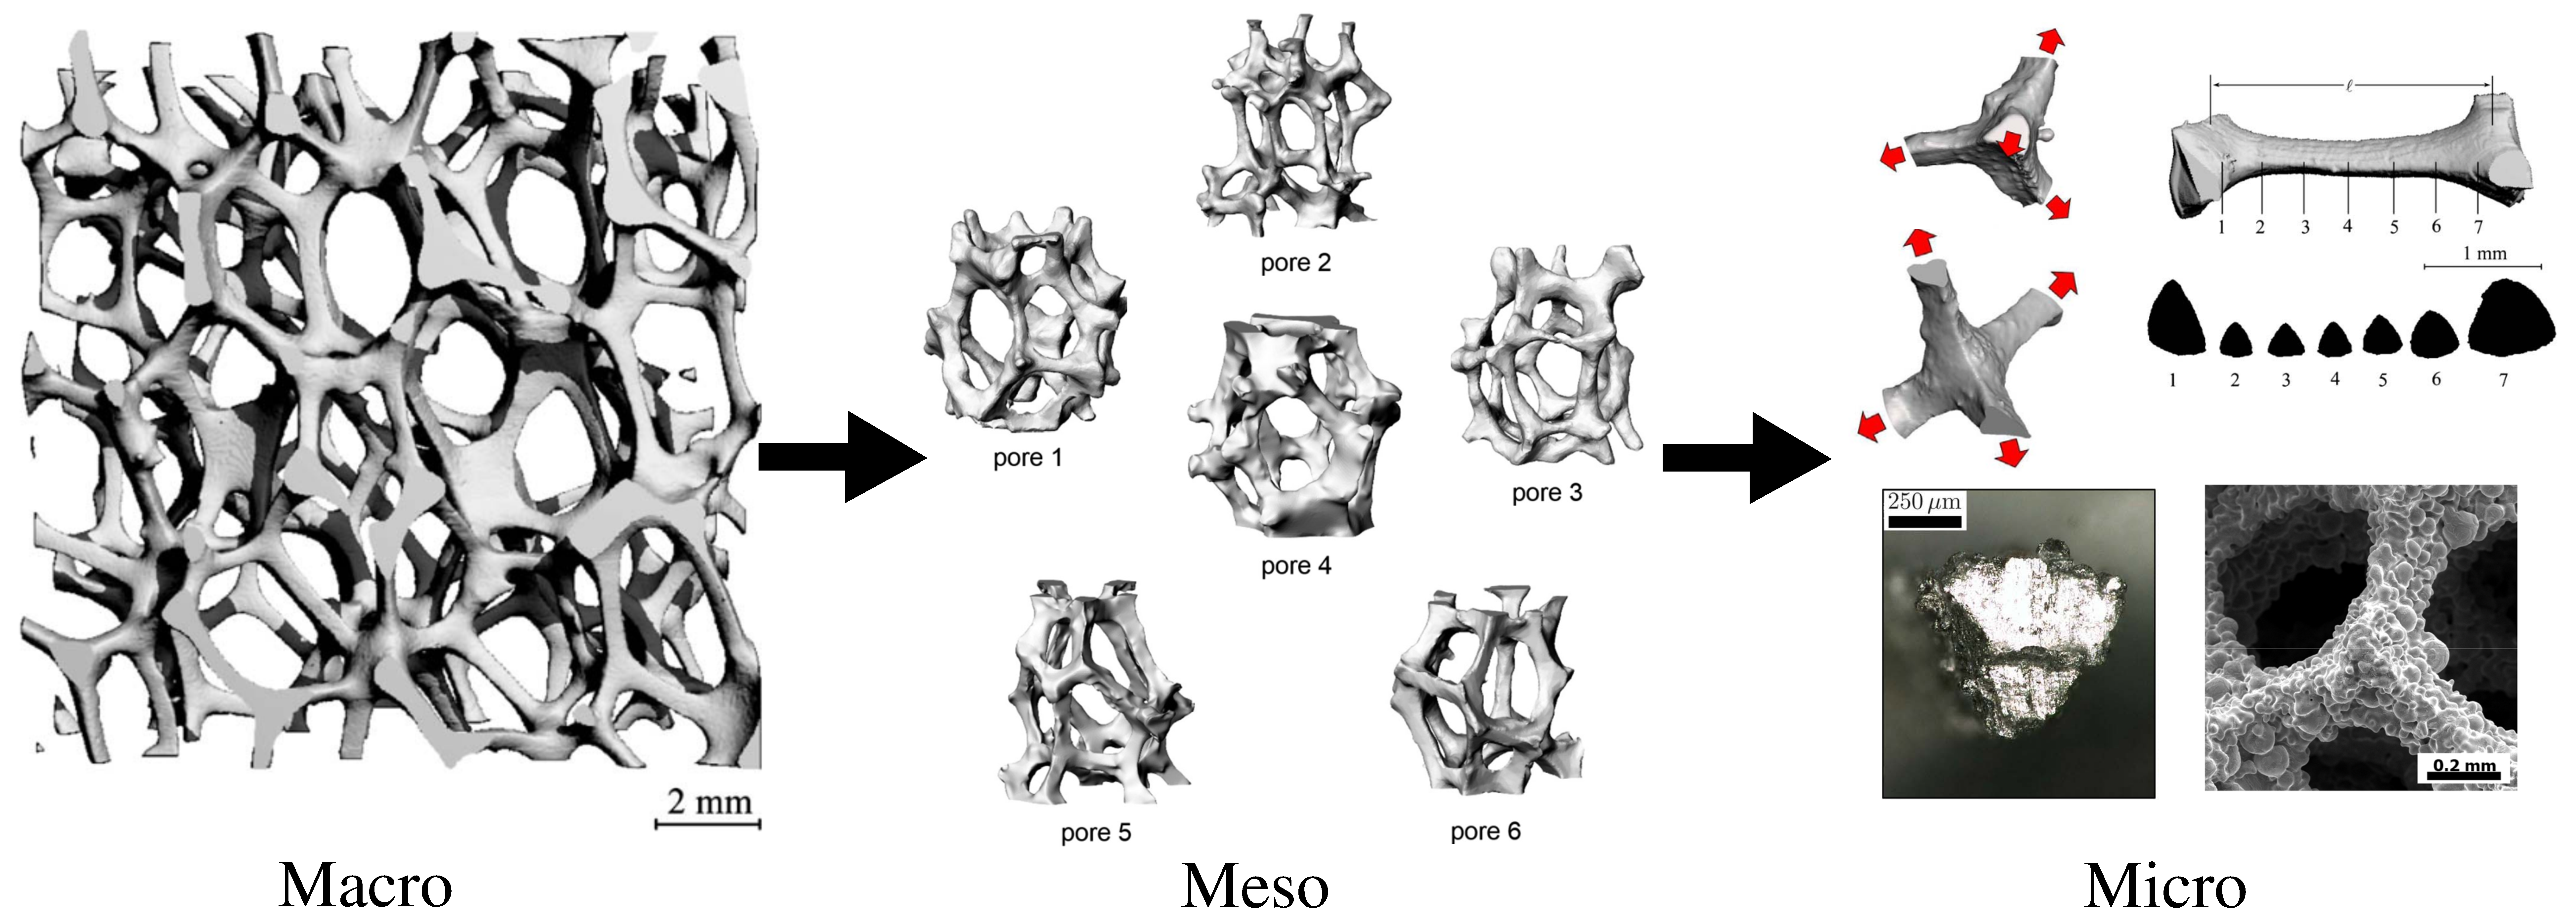
\includegraphics[width=\textwidth]{foam_scale}
	\end{subfigure}
\caption{Hierarchical scale based representation of the material. The units range from cm at macro scale to $ \mu $m at the micro scale. Images sourced from \cite{jangMicrostructureOpencellFoams2008,jungOpencellAluminiumFoams2015}}\label{fig-int-scale}
\end{figure}

Metal foams are micro-heterogeneous materials. It is possible to define the phenomenological description of the material properties using a multiple length scale based hierarchy (Figure \ref{fig-int-scale}). In such a description, the material can be divided into sub-levels that are considered homogeneous in a simulation and the properties at each individual sub-level depend only on the effective inhomogeneities at that sub-level. The sub-level that defines the micro-structure describes the structure of the struts of the foam, the grain size, voids and any inclusions in the strut. As one goes higher, the meso-scale characterizes the length and the thickness of the struts arising due to the varying cross-section and the resultant shape of the pores. At the highest level of homogenization, the macro-scale, several pores of the foam are covered and it is regarded as a continuum where the local damage and deformation mechanisms can not be investigated.

The material response of metallic open foams is characterized by the initial elastic increase in the stress with a small amount of local plastic deformations, followed by a stress plateau due to the successive collapse of the pores in the specimen, and finally a steep increase in the stress due to material densification (Figure \ref{fig-int-sample}(a)). It also becomes necessary to identify the bulk material properties of the individual strut elements so as to not over-estimate the stress-strain response leading to very high stiffness\cite{jungModellingMetalFoams2016}. A study on effective  micro-material properties has been presented in \cite{heinzeExperimentalNumericalInvestigation2018} (Figure \ref{fig-int-sample}) where the authors have identified effective micro-mechanical properties, i.e., the material properties of the struts of aluminium foams using inverse modeling techniques.

\begin{figure}
	\centering
	\begin{subfigure}{0.45\textwidth}
		\includegraphics[width=\textwidth]{only_data}
		\caption{}
	\end{subfigure}
	\begin{subfigure}{0.45\textwidth}
	\includegraphics[width=\textwidth]{foam_pore_samples}
	\caption{}
	\end{subfigure}
	\caption{(a) Experimental observations of the material response of some metallic open foam specimens as observed in \cite{jungMicrostructuralCharacterisationExperimental2017} during uniaxial compression. The zones of (1) elastic regime, (2) plateau regime and (3) densification regime has been labeled. (b) Material response of individual pores as observed in \cite{heinzeExperimentalNumericalInvestigation2018}. }\label{fig-int-sample}
\end{figure}

A numerical study of the material behavior of these open foam micro-structures can be carried out by a well structured computational homogenization scheme that takes the macro scale as a continuous homogeneous media while applying the constitutive behavior of the strut material on the micro-scale. This necessitates the ability to model the micro-structure by taking into account the various complexities that are observed in the physical foams that are in use. Idealization of the micro-structure by assuming it to visually be similar to various geometrical patterns assembled in a predictive or a periodic manner is an easy way to obtain the basic elastic properties of the foam structures. However, it is better if such models can statistically represent the general foam features by taking into consideration as few assumptions as possible to avoid the accumulation of errors resulting due to these assumptions on the macro behavior of the material model. These complexities can be obtained through the generation of tessellations based on random spherical packings.

Nevertheless, a detailed representation of the micro-structure often leads to an overwhelming computational cost. In recent times, significant progress has been done to reduce the computational cost of these computational homogenization procedures. The optimization can be achieved by either reducing the model complexity in what is known as reduced order modeling, but at the expense of complex numerical analysis, or by the advanced tools made available thanks to the progress in machine learning approaches like artificial neural networks. 

\section{Micro-structure representation}

A model structure, with repeated calculations with varying model parameters, allows investigating the changes in the overall material properties associated with changes in the micro-structure. 

In this regard, 3D characterization and modeling of real structural foams using computer tomography (CT) images can provide significant insight into the sample structure. These images can then be discretized and studied using finite element method (FEM) simulations \cite{veyhlFiniteElementAnalysis2011,fiedlerMCTbasedFiniteElement2012,fiedlerComputedTomographyBased2009}. Yet, this remains a daunting task since characterizing all the samples requires both time and processing capacity, thus restricting the analysis to smaller samples requiring user-assisted analysis of the images \cite{montminy3DStructureReal2004}. 

Another reconstruction methodology based on CT scan images has been presented in \cite{leblancAnalysisOpenFoamUnderPreparation} where the individual pores of the foam samples have been embedded with ellipsoids and polyhedrals. This method, while being computationally cheaper than the standard watershed algorithm\cite{lautensackFittingThreedimensionalLaguerre2008}, is also capable of implicitly capturing the anisotropy present in the foam samples that could be generated due to the manufacturing method used. 

Idealization of the geometry with the help of deterministic models such as the Kelvin\cite{thomsonLXIIIDivisionSpace1887} or the Weaire-Phelan\cite{weaireCounterexampleKelvinConjecture1994} was developed to obtain numerically derived models. To overcome the inability of these numerical models to capture the local variations occurring in the foam samples, random Laguerre tessellations generated by non-overlapping sphere packings were presented in \cite{redenbachMicrostructureModelsCellular2009}. A completely numerical approach based on sphere packing algorithms and an eventual surface minimization based approach to extract the foam micro-structure has been presented in \cite{kraynikStructureRandomFoam2004}. 

A novel approach was presented in \cite{sononAdvancedTechniquesGeneration2014} in which the authors make use of level sets and implicit surfaces represented by the direct and indirect usage of the level sets that are generated by points and arbitrarily shaped surfaces. From its use as a random packing generator to applications in textile fiber orientations, the level sets have the capability to represent various morphologies including cellular materials. With the help of discrete grids of points, the morphologies can be extracted as statistically Representative volume elements (RVE) that can then be used to study and analyze virtual models undergoing complex loading. The presence of distance functions and level sets enables the extraction of well defined and morphologically representative models of open foam structure that can be used conveniently as a micro-model in various analysis tools.

Any modeling tool that enables researchers to obtain better geometries of physical objects needs to be quantitatively as well as qualitatively analyzed. There are several studies in literature that look into the mechanical properties as well as the micro-structural geometries of open foam made of various materials, ranging from polyethylene, aluminum, titanium alloys to coated hybrid metal foams\cite{zhouInvestigationMicrostructureStrength2002,zardiackasStructureMetallurgyMechanical2001,sypeckStructureDeformationAluminum1998,stormInfluenceCurvedStruts2015,pangSynthesisMechanicalProperties2012}. To establish the usefulness of the geometry generator, it becomes necessary to compare the geometry of the randomly generated model to other existing modeling tools as well as physical studies on experimentally generated foam samples. In \cite{jungMicrostructuralCharacterisationExperimental2017}, the authors present a detailed analysis of the effect of the pore size on the material behavior while in \cite{heinzeExperimentalNumericalInvestigation2018}, this study has been conducted on single pore samples of the foam along with a study based on reconstruction of the geometry from computer tomography (CT) scan images and photogrammatry, or reconstruction based on photographs.

Finally, in order to use the extracted geometries in a well structured multi-scale computational homogenization strategy, the RVE geometry needs to be discretized into finite elements. An approach to generate conformal meshes from implicit surfaces was presented in \cite{ehabmoustafakamelIntegratedApproachConformal2019} which utilizes basic triangulation techniques provided by standard meshing tools and generates a refined mesh while maintaining the topological conformity. This mesh methodology will be adopted in the sequel.

\section{Multiscale methods}
The application of material characterization to a very detailed level is helpful in bridging the knowledge gaps that exist currently in the understanding of overall behavior of cellular materials and complementing real experiments with virtual testing means is very much the way forward in the field of study and analysis of complex micro-structures. Considering the fact that cellular materials exhibit complex mechanical behavior due to various issues like size-effect\cite{andrewsCompressiveTensileBehaviour1999} or localization phenomena due to micro-buckling of thin components like cell struts\cite{jangCrushingAluminumOpencell2009}, which strongly influences the structural stiffness, the study of the behavior of the cellular materials needs to be properly organized. In this regard, the detailed geometry of the structure after extraction can be studied using finite element formulations by direct numerical simulation (DNS) at the microscopic scale \cite{mangipudiMultiscaleModellingDamage2011,gibsonCellularSolidsStructure1997} which could possibly lead to a solution that needs a large number of unknowns to be considered. Another approach considers the cellular structure as a continuous medium on which a phenomenological model can be applied\cite{forestContinuumModelingStrain2005} called the macroscopic approach. This method while being efficient can not account for the complex geometries of the micro-structure. Also, the evolution of the micro-structure during the loading phase will not be captured. This brings attention on combining the two methods, where two separate Boundary Value Problems (BVP) are defined at two separate scales in a method also known as FE$ ^2 $. 

However, because of the complexities in the micro-structure, \fee simulations cannot be envisioned to study lightweight structures because of the current limitations in computational resources. 
%{A lot of times}, due to limitations of computational power necessary for the data processing of images extracted by standard CT scanners, one can only expect a very small sample of the foam to be imaged. This data may not always be sufficient to conduct an efficient RVE based computational analysis of the behavior and to address these kinds of issues, \cite{cottereauStochasticdeterministicCouplingMethod2013} discusses algorithms to couple a deterministic model to a random stochastic RVE based on a weak energy coupling operator. This model is able to circumvent the bias observed due to over-constraints introduced by the boundary conditions on the RVE.
At this juncture, one can make use of the computational tools developed in the software industries as well as the advancements in the electronics industries to find suitable solutions to reduce the computational cost and time involved in the classical multiscale methods. Reduced order basis and machine learning solutions can then be considered as an efficient surrogate in the multiscale computational homogenization process.

\section{Data driven analysis}

It is a consistent challenge to improve the efficiency of solvers that are used to analyze various behavioral traits of complex micro-structures, all while increasing the fidelity of the same micro-structure representation. The same problem recurs with the use of FE$ ^2 $ approaches where, to avoid the loss of generality, an embedded micro-model at each macroscopic integration gauss point can lead to extreme increase of the processing power needed. 

Model reduction strategies based on non-uniform transformation field analysis developed on the basis of principal component analysis\cite{michelModelreductionApproachMicromechanics2016,michelNonuniformTransformationField2003,jolliffePrincipalComponentAnalysis2014} or proper orthogonal decomposition\cite{yvonnetReducedModelMultiscale2007} have tried to circumvent the complexities, but at the expense of extensive \textit{a priori} simulations that are necessary to capture the complex behavior. Reduced order methods such as the manifold learning methods based on isomaps have also been studied for heterogeneous materials\cite{bhattacharjeeNonlinearManifoldbasedReduced2016}. However the applications of these methods for dependent plastic materials can be more challenging, either because of the time required to evaluate the local constitutive laws for the former family, or due to the difficulty to frame the history dependency for the latter ones.

To reduce the burden on the processors and to not give away the efficiency, it would be interesting to look towards the efforts made in data mining and artificial intelligence fields and go through various data driven models as surrogates or supporting tools in FE$ ^2 $ analysis which could be capable of dramatically accelerating the scheme.

A distance-minimizing based scheme has been presented in \cite{kirchdoerferDatadrivenComputationalMechanics2016} that can be construed as the beginning of a renewed interest on data driven solvers to accelerate multi-scale analysis. The scheme presented tries to find a corresponding point in the material dataset that tries to minimize the error while trying to satisfy the essential boundary conditions, avoiding the need for constitutive material model. Moving on to large deformations, material data has been presented in a lower dimension and a hidden constitutive manifold is attempted to be solved by following an adaptive search direction\cite{chinestaDataDrivenComputationalPlasticity2017}. In \cite{bessaFrameworkDatadrivenAnalysis2017}, the authors have developed a data-driven computational framework that approximates the relationship between the key descriptors of each design and the quantities of interest to address the issue of high dimensionality of the problems. 

The current level of progress achieved in the artificial intelligence has led to a very focused interest on machine learning based models, such as artificial neural networks (ANN) and deep learning, with respect to their applicability to study the mechanics of materials\cite{bessaFrameworkDatadrivenAnalysis2017,ghaboussiAutoprogressiveTrainingNeural1998,ungerNeuralNetworksMaterial2009,wangMultiscaleMultipermeabilityPoroplasticity2018}. ANNs in specific, also known as connectionist systems, are computing systems that are vaguely inspired by the biological neural networks\cite{chenDesignImplementationCloud2019}. These systems can be trained to ``learn" particular tasks without any specific programming with task-specific rules. A simple example, from the field of image recognition, is when a set of images manually labeled with ``car" and ``no car" can be trained to predict whether a car is present or not in a new image without any specific programming to recognize car specific features like tires, doors, or the shape of the car. The ANNs can do this simply by generating identifying characteristics from the examples that they process.

However, it is very necessary to know beforehand that the data driven tools are developed depending on the specific problem, and may not work very well beyond the original sampling space, in particular for different material laws and loading paths. Significant work is also necessary to tackle history dependency, physical invariance and conservation laws as the models do not consider the physics of the behavior and simply predict based on mathematical and statistical calculations.

ANNs have the advantage of being versatile in their design and thus form a very useful tool in the quest to surrogate efficiently an FE$^2$ analysis. Ranging from a simple multi-layer perceptron to deep neural networks\cite{haykinNeuralNetworksLearning2009}, ANNs have changed the modern digital computing age, and the abundance of available data on various aspects of human life through simple click of a smartphone button, influencing the technology that brings humanity various conveniences like linguistic translation to assisted-driving. Unfortunately, the abundance of data required to train the ANN cannot be extracted experimentally. But the availability of modeling tools has presented a curious case of an abundance of virtual data that can be used instead. It then becomes imperative that the virtual data used to train the ANN models are of satisfactory quality. The non-linearities present in complex micro-structure ensures that the training process of the virtual data is not a cakewalk and needs constant studying so as to not generate a myriad of garbage predictions\cite{rochaMicromechanicsbasedSurrogateModels2020}.

When it comes to applications of ANNs on fields related to mechanics, there have been some considerable recent works that can be found in literature. ANNs have been used to replace some of the parts of  material constitutive  laws in \cite{furukawaImplicitConstitutiveModelling1998,furukawaAccurateCyclicPlastic2004,wangMetamodelingGameDeriving2019}, and as FE surrogates in \cite{lefikArtificialNeuralNetwork2003,hashashNumericalImplementationNeural2004,zhangUsingNeuralNetworks2020}. In \cite{wuBayesianInferenceNonlinear2020}, the authors have used ANNs to substitute complex material computational homogenization constitutive laws in order to obtain an accelerated computational scheme in the context of the Bayesian inference of the micro-scale parameters.

Expanding this knowledge to \fee analysis can be done in various ways. Simple sequential feed forward networks (FNNs) have been found to be quite useful in their role as surrogates in computational homogenization procedures, as can be found in \cite{leComputationalHomogenizationNonlinear2015,bessaFrameworkDatadrivenAnalysis2017} where the strain energy density surface has been approximated, or in \cite{fritzenOntheflyAdaptivityNonlinear2019,ungerCouplingScalesMultiscale2008,settgastHybridApproachSimulate2020} where the stress-strain responses have been approximated. Specifically in \cite{settgastHybridApproachSimulate2020}, the micro-scale plastic strains have been used as state variables updated at each loading step in combination with an FNN. However, in cases like elasto-plasticity, where history dependent plasticity is induced in complex micro-structures, it may not be easy to define these state variables.

With the aim of accounting for history dependency, in \cite{ghavamianAcceleratingMultiscaleFinite2019}, recurrent neural networks (RNNs), specifically long short term memory (LSTM) cell based networks were used to study 1D elasto-visco-plastic cyclic loading conditions. In \cite{wuRecurrentNeuralNetworkaccelerated2020,gorjiPotentialRecurrentNeural2020}, gated recurrent unit (GRU) cell based networks have been used to represent micro-scale responses of 2D RVEs under non-proportional loading and have been found to be more efficient.

\section{Objectives of the present work}

In this work, new methodologies have been developed in order to study the response of open foam metallic structures. 

Firstly, an effort has been put to represent open foam morphologies, keeping in mind the geometric constraints and model refineness using level sets and distance functions. Particular focus has been put on capturing the intricacies of the strut geometry so as to capture deformations like buckling that influence the overall foam properties. The generated RVE can then be used in a multi-scale analysis as the micro-scale geometry that influences the macroscopic homogenized behavior of the RVE. \red{A methodology to develop sharp edges of the open foam struts has been presented with the help of a multiple level-set based approach. The entire tool has been presented such that both random geometries as well as reconstruction of geometries based on CT scans of open foam physical samples can be conducted.}

To validate the accuracy of the models thus developed, a study has been done by comparing the virtual behavior with that of an actual sample, the computed tomography (CT) scans of which have been used as a seed to generate the RVE. Various tools and techniques that have been used to generate these morphologies are explained in detail. 

To speed up the computational efficiency of the multi-scale analysis of such complex geometries, various data-driven models have been studied. Considering 2D structures as proof of concept, a surrogate has been developed that uses ANNs to boost up the performance of computation from simple architecture. Relevant mechanical theory to obtain the aforementioned efficiency has been sketched out in detail to demonstrate the ability of the surrogate. The problems faced and the possible solutions to overcome these problems have also been studied and mentioned here so as to present an accurate picture of the current state of art, its abilities and its shortcomings.

This work is organized as follows:
\begin{itemize}
	\item In Chapter \ref{chap-ch}, \textit{\titlech}, a computational homogenization scheme based on multi-scale analysis is presented that uses a first order based approach to formulate the relevant theory behind the homogenization process. Use of relevant boundary conditions to formulate the BVP has been discussed. 
%	In particular, a description of a self-consistent coupling algorithm is also presented where the elasto-plastic model applied on the RVE is coupled to an embedded media that behaves based on a polynomial hyper-elastic based model.
	\item In Chapter \ref{chap-of}, \textit{\titleof}, a distance neighbor based packing algorithm is developed that can implicitly generate morphologies. Functions necessary to extract open foam morphologies from the distance functions generated are presented along with various tools necessary to extract strut geometries. An efficient method to reconstruct morphologies from CT scans is also presented and tools necessary to post-process these image-based morphologies are discussed. Finally, the extraction of finite element models based on the contours generated by the various distance fields are presented.
	\item In Chapter \ref{chap-res}, \textit{\titleres}, discussions on the morphologies extracted from the distance neighbor based algorithm are presented. Statistical validation of the morphologies along with the study of their mechanical behavior is discussed. A virtual model extracted based on this work is compared with a physical model extracted from CT scan images along with discussions on their respective effectiveness and shortcomings due to application of various boundary conditions.
	\item In Chapter \ref{chap-nn}, \textit{\titlenn}, a study on ANNs is developed that details the current state-of-the-art in the field of computational homogenization and data-driven solvers. Some possible surrogate neural networks are studied and compared that can be used in large scale prediction of virtual behavior and possibly in the future on experimental behavior. ANN models based on a combination of Feedforward Neural Networks (FNN) and Recurrent Neural Networks (RNN) are presented to conduct material analysis with history-dependent behavior that can be implemented in an FE$^2$ setting.
\end{itemize}

\section{Contributions}

The contributions of this work are as follows:
\begin{enumerate}
	\item Starting from works presented in \cite{sononAdvancedApproachGeneration2015}, a geometrical tool has been developed that can model the micro-structure of open cell foams using distance fields and level sets taking into account various features like the struts cross-section evolution, etc. \red{A methodology has been developed that takes into account multiple level sets calculated as a function of different distance fields and generates sharp edges corresponding to the open foam struts which was missing. The developed tool then refines the surface mesh extracted from these modified level sets and generates a tetrahedral mesh form of the geometry. Also, the implicit extraction of strut geometry variations is described in detail.} The resulting micro-structures have been validated through statistical indicators like the number of pores, faces, etc. The homogenized material behavior of the foam model thus generated have been statistically validated against experimental observations. 
	\item An efficient way to reconstruct the geometry of open foams from CT scans has been developed that can also store the required distance fields implicitly. A computationally cheaper method to obtain inclusion packing from CT-scan has been presented in \cite{leblancAnalysisOpenFoamUnderPreparation} which has been used as the base packing to develop distance fields. \red{Thus, starting from CT-scan images, an extension has been developed that builds distance fields and level sets that can then be used to build back the open foam geometry in the form of tetrahedral mesh.} The developed foam model behavior has been compared with the corresponding experimental observations to understand the utility of the reconstruction strategies. 
	\item A machine learning study has been conducted and various neural network based models have been tested as efficient surrogates during the computational homogenization process. \red{In this regard, various artificial neural networks like feedforward neural networks and recurrent neural network modules are prepared, trained to predict homogenized behavior of open foam morphologies and tested against direct numerical solution based results.} The developed models have been compared with the traditional FE methods at the micro-scale to obtain the material behavior and understand the complexities and the shortcomings involved in data driven approaches with respect to computational mechanics.
\end{enumerate}

\section{Publications}

This work has directly resulted in the publication of the following article in peer reviewed journal as main author:
\begin{itemize}
	\item N. G. Kilingar, K. Ehab Moustafa Kamel, B. Sonon, T. J. Massart, and L. Noels.
	Computational generation of open foam representative volume elements with morphological control using distance fields. 
	European Journal of Mechanics - A/Solids,
	page 103847, September 2019;
\end{itemize}
and as co-author:
\begin{itemize}
	\item L. Wu, V. D. Nguyen, N. G. Kilingar, and L. Noels. 
	A recurrent neural network accelerated multi-scale model for elasto-plastic heterogeneous materials subjected to random cyclic and non-proportional loading paths.
	Computer Methods in Applied Mechanics and Engineering, 
	369:113234, September 2020.
	\item C. Leblanc, N. G. Kilingar, A. Jung, K. Ehab Moustafa Kamel, T. J. Massart, E. Bechet, and L. Noels. 
	Development of open-foam morphologies by reconstructing CT-scan images.
	In preparation.
\end{itemize}
This work has been presented at the following international conferences:
\begin{itemize}
	\item Nanda Gopala Kilingar, Ludovic Noels, Karim Ehab Moustafa Kamel, Bernard Sonon,
	and Thierry Jacques Massart. Generation of open foam RVEs with sharp edges using Distance fields and Level sets. In ECCOMAS Thematic Conference on Computational modeling of Complex Materials across the Scales - CMCS 2017, November 2017.
	\item Nanda Gopala Kilingar, Ludovic Noels, Karim Ehab Moustafa Kamel,
	and Thierry Jacques Massart.
	Generation Of open foam RVEs
	With Strut Variations Using Distance Fields And Level Sets.
	In
	The 9th International Conference on Computational Methods
	(ICCM2018), June 2018.
	\item Nanda Gopala Kilingar, Ludovic Noels, Thierry Jacques Massart, Karim Ehab
	Moustafa Kamel, Bernard Sonon, Christophe Leblanc, and Anne Jung. Data
	driven computational analysis of open foam RVEs. In Computational Methods in Multiscale, multi-uncertainity and multi-physics problems conference
	CM3 2019, July 2019.
\end{itemize}
%\textit{}
\afterpage{\clearpage}
\clearemptydoublepage

% Draft Version 1 - Date 16/06/2020
% Draft Version 2 - Date 06/08/2020
% Draft Version 3 - Date 27/08/2020
% Draft Version 4 - Date 23/09/2020
% Draft Version 5 - Date 14/12/2020

\chapter{\titlech}\label{chap-ch}

\section{Introduction}
Every material found in nature has heterogeneity involved at different scales of length. This heterogeneity results in complex behavior leading to a significant impact on the material properties and the inherent response to different loading conditions. The prediction of the behavior due to these spatial variations in the material can be directly computed using direct numerical simulation of the finite element discretization of the heterogeneity. But any such approach needs to ensure that the mesh size is comparatively smaller than the size of the heterogeneity, leading to significant computational cost due to the enormous number of degrees of freedom. However, this does not negate the importance of taking into consideration the various high accuracy geometry development tools to study complex material structures in high performance applications.

Homogenization techniques have traditionally been used to extract effective macroscopic properties of such heterogeneous media. Semi analytical methods such as mean field homogenization (MFH) based on Eshelby tensor\cite{pierardMeanfieldHomogenizationMultiphase2004}, 
%asymptomatic homogenization theory\cite{bensoussanAsymptoticAnalysisPeriodic2011}, Bloch wave homogenization\cite{allaireComparisonTwoscaleAsymptotic2016}, 
among others, are usually restricted to simple microscopic geometries and simple material models, often under the assumption of small strains. The concept of a unit cell to determine the homogenized material properties by fitting the detailed modeling of the unit cell on macroscopic phenomenological equations was developed in \cite{hillElasticPropertiesReinforced1963} and was used to display the effectiveness of such unit cells in various studies\cite{christmanExperimentalNumericalStudy1989,tvergaardMechanicalModellingDuctile1991,baoImprovedTn7basedSystem1991,brockenbroughDeformationMetalmatrixComposites1991}. The extension of the unit cell to a history dependent constitutive behavior through micro-macro behavior can be obtained in an efficient manner by assigning a unit cell to each integration point of the macro-mesh\cite{smitPredictionMechanicalBehavior1998} and this procedure can be called homogenization based multi-scale analysis.

Multi-scale and homogenization techniques have been used to predict the collective multi-phase response of materials on the basis of the understanding of single phases and complex interfaces in materials along with the taking into account of large deformations, damage, cracking and phase transformations among other mechanical effects \cite{geersMultiscaleComputationalHomogenization2010}. Among these, computational homogenization is probably one of the most accurate techniques in upscaling the non-linear behavior of well characterized micro-structure. In this method, a computational boundary value problem (BVP) is constructed which is then numerically solved to determine the local governing behavior at the macro scale. A fully nested solution of BVP at each scale is obtained if the macro scale BVP is solved simultaneously (Figure \ref{fig-ch-homogenization}). For a  periodic micro-structure, a unit cell can be used to define the micro BVP, while a Representative Volume Element (RVE) has to be used for non-periodic ones. In the latter case, it is necessary to ensure that the RVE size is large enough to represent statistically the pertinent information of the micro-structure. Considering that larger RVEs will result in higher computation times, the critical size of the RVE needs to determined taking into account efficiency and accuracy\cite{ostoja-starzewskiMechanicsRandomMaterials2001,kanitDeterminationSizeRepresentative2003}. It is also necessary to note that a volume element becomes a true RVE only when the effective constitutive response is independent with respect to the boundary conditions that are energetically consistent, which can be satisfied by the Hill-Mandel principle.

\begin{figure}
	\centering
	\begin{subfigure}[t]{0.75\textwidth}
		\includegraphics[width=\textwidth]{homogenization_1}
	\end{subfigure}
	\caption{First order computational homogenization of continua.}\label{fig-ch-homogenization}
\end{figure}



This chapter will briefly recall the first order computational homogenization scheme. A periodic boundary condition (PBC) based boundary value problem will be explained that can be used in existing solvers. 
%A self-consistent based homogenization scheme is finally presented that can help avoid boundary effects on RVEs due to the geometrical constraints induced by the RVEs reconstructed from CT-scans of open foam structures, and the reconstruction strategy explained in Chapter \ref{chap-of}. 

The chapter is outlined as follows: In Section \ref{ch-first}, a first order computational homogenization scheme is presented. The corresponding macroscopic formulations, the microscopic formulations and the scale transitions are explained. In Section \ref{ch-periodic}, a PBC based system to solve the boundary value problem presented in Section \ref{ch-first} is explained. In Section \ref{ch-matrices}, the kinematic matrices and their resolution is outlined. 
%Section \ref{ch-self} presents a self consistent homogenization scheme to take into account RVEs that are small in size and for which PBC cannot be directly applied. 

\section{First order computational homogenization}\label{ch-first}

The basic principle of the first order homogenization of mechanical problems is highlighted in Figure \ref{fig-ch-homogenization} where the scale transitions between the two scales are indicated. The deformation gradient, $\textbf{F}_\text{M}$, that constitutes the macroscopic kinematical quantities in this case, is transferred to the micro-scale in order to define a BVP on the RVE. By solving the microscopic BVP in the standard manner, a deformed RVE with corresponding boundary displacements and surface traction is obtained. By making use of standard mathematical averaging equations, the macroscopic stress tensor, $\textbf{P}_\text{M}$, can be extracted. To solve the macroscopic BVP  in parallel, static condensation process can be used to obtain the tangents from the RVE stiffness. This method is also denoted as \fee \cite{feyelFE2MultiscaleApproach2000,feyelMultilevelFiniteElement2003} when the finite element method is used at both scales to solve the entire problem as a nested BVP.

%If we consider the macroscopic nonlinear deformation map, $\mathcal{F}(\tgm[]{X})$, applied to a material vector $\tgm[]{u}$ in the deformed state, then the first order scheme can be written as 
%\begin{equation}
%\tgm[]{u}=\left({\tgm[]{F}-\textbf{I}}\right)\boldsymbol{\cdot}\tgm[]{X}+\tgmm{w}\label{eq-ch-order1}
%\end{equation}
%with $\tgm[]{X}$ and $\tgm[]{X}'$, the associated position vectors in the reference and deformed states respectively, $ \tgm[]{u} $ the reference displacement field and such that $\tgm[]{F}=(\bm\nabla_0\tgm[]{X})^T$. The subscript M represents the macroscopic values. The vector $\tgmm{w}$ represents the micro-fluctuation field that takes into account the local fine scale contribution which is different from the macro-scale deformation\cite{geersMultiscaleComputationalHomogenization2010}. Eq. (\ref{eq-ch-order1}) is valid in every point at the fine scale. In the following subsections, a scale transition from the micro-scale to the macro-scale will be defined to comprehensively link the various stages of computational homogenization.

\red{The separation of scales is an important assumption that can be described as \textit{the microscopic length being much smaller than the characteristic length over which the macroscopic loading varies in space}, i.e.,
\begin{equation}
l_{micro}<<<l_{RVE}<<<l_{macro}
\end{equation}
where $ l_{micro} $ denotes the average size of the pores, inclusions, or grains of the crystals forming the material, $ l_{RVE} $ denotes the size of the RVE and $ l_{macro} $ denotes the characteristic length over which the macro field varies. The condition, $ l_{micro}<<<l_{RVE} $, ensures the statistical representativeness of the micro-scale BVP, while the condition, $ l_{RVE}<<<l_{macro} $, ensures that the average deformation gradient applied on the RVE is meaningful. This also implies that the method is severely limited in the first order case to analyze localization problems since in the latter case $ l_{macro} $ can become smaller than the RVE size, in effect resulting in the loss of the representativeness of the RVE. As a result, the average stress-average strain relationship loses size objectivity beyond strain softening onset. For example, to deal with the problem of failure, other quantities like dissipation energy can be used to characterize the softening homogenized response\cite{nguyenMicromechanicalModelReinforced2019}, or a second order scheme be implemented to handle buckling\cite{nguyenComputationalHomogenizationCellular2014}. However, this second order scheme results in the non-physical problem of persistent gradient effect when the considered RVE is homogeneous, i.e., the response depends on the size of the RVE. A correction, based on micro-structure-dependent body force field can be implemented in the homogenization field along with alternative definitions of localization tensors\cite{yvonnetComputationalSecondorderHomogenization2020,monchietStraingradientHomogenizationBridge2020}. Another class of homogenization, consists of generalized micromorphic continuum that results in an extended continuum at macro-scale by suitable decomposition of the displacement field\cite{rokosExtendedMicromorphicComputational2020,vanbreeNewtonSolverMicromorphic2020}.

However for most of the situations, a first order formulation is sufficient and is a standard tool in computational homogenization\cite{matsuiTwoscaleFiniteElement2004,mcveighMultiresolutionAnalysisMaterial2006,temizerNumericalMethodHomogenization2007,hainComputationalHomogenizationMicrostructural2008}.In this work, we will see that when studying 3D open foam structures in Chapters \ref{chap-of} and \ref{chap-res}, the RVE responses do not exhibit strain softening, justifying the use of the first order homogenization. When considering 2D foam-like structures in Chapter \ref{chap-nn}, a limited softening can be observed before the plateau response, but we consider first order homogenization as an illustration of the data-driven approach, although it should rigorously be extended to a higher order formulation.}

\subsection{Macroscopic formulation}\label{ch-form-macro}
The macro-scale kinematics are defined by the deformation gradient $\tgm[]{F}=\textbf{I}+\tgm[]{u}\otimes\bm\nabla_0$ 
%and its gradient $\tgm[3]{G}=\tgm[]{u}\otimes\bm\nabla_0=\tgm[]{u}\otimes \bm\nabla_0\otimes\bm\nabla_0$
with $ \tgm{u} $ the reference displacement field and $ \bm\nabla_0 $ the gradient operator with respect to the reference configuration. In the absence of body and inertial forces, the strong form of the continuum equilibrium is represented in the body $\Omega$ by
\begin{equation}
	\tgm[]{P}(\tgm[]{X})\cdot\bm\nabla_0
	%-\tgm[3]{Q}(\tgm[]{X}):(\bm\nabla_0\otimes\bm\nabla_0)
	=0,\,\,\,\,\forall\tgm[]{X}\in\Omega.\label{eq-dG-macro}
\end{equation}
where $ \tgm{X} $ is a material point of the body $ \Omega $ expressed in the reference configuration and seen as homogeneous. The boundary conditions read
\begin{subequations}\label{eq-dG-Macro_bc}
	\begin{align}
	\tgm[]{u}(\tgm[]{X}) & =\tgm[]{u}^0, & \forall\tgm[]{X}\in\partial_D\Omega,\\
	\tgm[]{T}(\tgm[]{X}) & =\tgm[]{T}^0, & \forall\tgm[]{X}\in\partial_N\Omega,
%	\text{D}\tgm[]{u}(\tgm[]{X}) & =\text{D}\tgm[]{u}^0, & \forall\tgm[]{X}\in\partial_T\Omega,\\
%	\tgm[3]{R}(\tgm[]{X}) & ={\tgm[3]{R}}^0, & \forall\tgm[]{X}\in\partial_M\Omega,
	\end{align}
\end{subequations}
with constrained displacement $\tgm[]{u}$ on the Dirichlet boundary $ \partial_D\Omega $ and traction per reference unit surface $\tgm[]{T}$ on Neumann boundary $ \partial_N\Omega $
%, and the high order boundary conditions of normal gradient of displacement $\text{D}\tgm[]{u}$ and of double traction per reference unit surface $\tgm[3]{R}$
. Also, 
\begin{equation}\label{eq-DG-bc_exp}
		\tgm[]{T}  = 
		\tgm[]{P}
		\cdot\bar{\mathbf{N}}_\text{M},
\end{equation}
where $\bar{\mathbf{N}}_\text{M}$ is the outward normal in the reference configuration. The stress divergence problem Eq. (\ref{eq-dG-macro}) along with the boundary condition (\ref{eq-dG-Macro_bc}) is completed by the respective constitutive law specifying the stress strain relationships at time $ t $:
\begin{equation}\label{eq-dG-const_macro-1}
	\tgm[]{P}(t) = \mathcal{P}_M\left\{\tgm[]{F}(\tau)
	%,\tgm[3]{G}(\tau)
	,\,\,\tau\in\left[0,t\right]\right\}.
	%\\
	%\tgm[3]{Q}(t) & = \textfrak{Q}\left\{\tgm[]{F}(\tau),\tgm[3]{G}(\tau),\,\,\tau\in\left[0,t\right]\right\}
\end{equation}

The relation (\ref{eq-dG-const_macro-1}) can be represented by introducing the internal state variables $ \tgm[]{Z} $ that denote the representation of the state of the material following the evolution laws of the internal state, with 
\begin{equation}\label{eq-dG-const_macro}
\tgm[]{P}(t) = \mathcal{P}_M\left\{\tgm[]{F}(t),\tgm[]{Z}(t)\right\}.
\end{equation}
The couple $ (\tgm[]{F},\tgm[]{Z}) $ gives a complete description of the constitutive behavior of the state space, and $ \tgm[]{P} $ is an observable quantity. This form of representation can be useful to understand the nature of the material at any given state without having the need to keep the full historical behavior of the material under observation. A general elastic law does not require the use of $ \tgm[]{Z} $.

The weak form corresponding to the system defined by Eqs. (\ref{eq-dG-macro}), (\ref{eq-dG-Macro_bc}) and (\ref{eq-dG-const_macro-1}) can be defined using an admissible kinematic vector field $ \textbf{U}(\Omega) $, where
\begin{equation}\label{eq-dG-law1}
\textbf{U}(\Omega)=\{\delta\tgm{u}\in\mathcal{H}(\Omega)\quad|\quad\delta\tgm{u}|_{\partial_D\Omega}=0\},
\end{equation}
with $ \mathcal{H} $ being the Hilbert space, and the weak form can be summarized as finding $ \tgm{u}\in\mathcal{H}(\Omega) $ such that
\begin{equation}\label{eq-dG-bilinear}
\int_\Omega\left[\tgm{P}(\tgm{u}):\tgm{P}(\delta\tgm{u})\right]\,d\Omega=\int_{\partial_N\omega}\tgm{T}^0\cdot\delta\tgm{u}\,d\partial\Omega\quad\forall\delta\tgm{u}\in\textbf{U}(\Omega)
\end{equation}
with the test function $ \delta\tgm{u} $.

In the context of computational homogenization, the constitutive relationship Eq. (\ref{eq-dG-const_macro}) can be obtained by resolving a microscopic BVP as explained below.

\subsection{Microscopic classical continuum}\label{ch-form-micro}
At the micro scale, the classical continuum assumption is applied. A separation of scale is assumed and the characteristic length of the microscopic BVP is much smaller than that of the continuum scale loading. The BVP is defined on an RVE $ \omega $ of boundary $ \partial\omega $ with the microscopic deformation gradient at a material point $ \tgmm[]{x}\in\omega $ in the reference configuration defined by
\begin{equation}\label{eq-micro-0-1}
\tgmm[]{F}=\textbf{I}+\tgmm[]{u}\otimes\bm\nabla_0,
\end{equation}
where the subscript m represents the local fields of the micro-scale, with the micro-scale reference  displacement field $ \tgmm[]{u} $ and gradient operator $ \bm\nabla_0 $. In the absence of the body sources, the equilibrium state is governed by the following relations,
\begin{equation}\label{eq-micro-1}
\tgmm[]{P}(\tgmm[]{x})\cdot\bm\nabla_0=\bm{0}\,\,\,\,\forall\tgmm[]{x}\in\omega,
\end{equation}
and
\begin{equation}\label{eq-micro-1-1}
\tgmm[]{P}(\tgmm[]{x})\cdot\bar{\mathbf{N}}_\text{m}=\tgmm[]{T}\,\,\,\,\forall\tgmm[]{x}\in\partial\omega,
\end{equation}
with the microscopic first Piola-Kirchhoff stress tensor $ \tgmm[]{P} $, the surface traction per unit surface $ \tgmm[]{T} $ on boundary $ \partial\omega $.
The boundary conditions directly result from the macroscopic variables and the microscopic fluctuations of the displacement field $ \tgmm{w} $ are defined as
\begin{equation}\label{eq-micro-2}
\tgmm[]{w}=\tgmm[]{u}-\left(\tgm[]{F}-\textbf{I}\right)\cdot\tgmm[]{x},
%-\frac{1}{2}{\tgm[3]{G}}:\left(\tgmm[]{x}\otimes\tgmm[]{x}\right)
\end{equation}
which helps achieving the scale transition (Figure \ref{fig-ch-micro}).
\begin{figure}
\centering
\begin{subfigure}[t]{0.75\textwidth}
	\includegraphics[width=\textwidth]{micro_bvp}
\end{subfigure}
\caption{Deformation of an RVE $ \omega $.}\label{fig-ch-micro}
\end{figure}
The continuum problem (\ref{eq-micro-1}) and its boundary condition (\ref{eq-micro-2}) is completed by a stress-strain relationship defined by a constitutive law at time $ t $
\begin{equation}\label{eq-micro-3-1}
\tgmm[]{P}(t)=\mathcal{P}_m\{\tgmm[]{F}(\tau),\tau\in\left[0,t\right]\}.
\end{equation}
With the introduction of a history-dependent vector $ \tgmm[]{Z} $, Eq. (\ref{eq-micro-3-1}) can be rewritten as
\begin{equation}\label{eq-micro-3}
\tgmm[]{P}(t)=\mathcal{P}_m\{\tgmm[]{F}(t),\tgmm[]{Z}(t)\}.
\end{equation}
In the case of an elasto-plastic material, as it will be used further in this work, this relationship is explicated in Appendix \ref{app-j2} and  \cite{nguyenComputationalHomogenizationCellular2014}.

The weak form corresponding to the system defined by Eqs. (\ref{eq-micro-1}) and (\ref{eq-micro-1-1}) can be defined using a kinematic vector field $ \textbf{U}(\omega)\subset\mathcal{H}(\omega) $, that will be defined during the scale transition.
%\begin{equation}\label{eq-micro-4}
%\textbf{U}(\omega)=\{\delta\tgmm{w}\in\mathcal{H}\left(\omega\right)\quad|\quad\delta\tgmm{w}|_{\partial\omega=0},
%\end{equation}
The weak form can be summarized as finding $ \tgmm{w}\in\textbf{U}(\omega) $ such that
\begin{equation}\label{eq-micro-5}
\int_\omega\tgmm{P}:\left(\delta\tgmm{w}\otimes\bm\nabla_0\right)\,d\omega=\bm{0},\quad\forall\delta\tgmm{w}\in\textbf{U}(\omega),
\end{equation}
with the test function $ \delta\tgmm{w} $.

The analysis of open foam materials involves deformation of individual struts of the RVE which calls for the treatment of surfaces and edges in contact. In this regard, a simple penalty based method has been introduced considering the particular advantage of explicit removal of constraint from the variational formulation leading to an unconstrained optimization\cite{laursenComputationalContactImpact2003}. This problem can be summarized as the addition of $ \Pi^c $ the contact contribution term to the strain energy. Supposing that two surfaces $ \partial\omega_1 $ and $ \partial\omega_2 $ of the body $ \omega $ come into contact, then the value of $ \Pi^c $ can be defined such that
\begin{equation}\label{eq-penalty}
\Pi^c = \frac{1}{2}\int_{\partial_C\omega}\epsilon\,(u_g)^2\,d\partial\omega
\end{equation}
where $ \epsilon>0 $ is the penalty parameter, $  \partial_C\omega $ the domain over which contact action takes place and 
\[ u_g=(\textbf x_2+\textbf{u}_2-\textbf x_1-\textbf{u}_1)\cdot\textbf{n}_1 \ge0\]  
represents the gap between the two surfaces with the unit normal vector $\textbf{n}_1$ defined on the current surface $ \partial\omega_1 $. The master point $ \textbf x_1\in\partial\omega_1 $ is considered as the orthogonal projection of a given slave point $ \textbf x_2\in\partial\omega_2 $ onto the master surface $ \partial_C\omega $ in the deformed configurations characterized by the respective displacements $ \textbf{u}_1 $ and $ \textbf{u}_2 $\cite{wriggersComputationalContactMechanics2006}. The variation of Eq. (\ref{eq-penalty}) gives
\begin{equation}\label{eq-penalty-2}
C_c=\int_{\partial_C\omega}\epsilon\,u_g\,\delta u_g\,d\partial\omega.
\end{equation}
The discretization of the penalty function is explained in detail in \cite{wriggersComputationalContactMechanics2006}.

\subsection{Scale transition}\label{ch-form-scale}

The scale transition can be complemented by two averaging equations:
\begin{enumerate}
	\item volume averaging of the deformation $\textbf F_\text M$ or stress $\textbf P_\text M$, defined as
	\begin{equation}\label{eq-st-1}
	\tgm[]{F}=\frac{1}{\omega}\int_\omega\tgmm[]{F}d\omega,
	\end{equation}
	and,
	\begin{equation}\label{eq-st-2}
	\tgm[]{P}=\frac{1}{\omega}\int_\omega\tgmm[]{P}d\omega;
	\end{equation}
	\item the Hill-Mandel macro-homogeneity condition, or the volume averaging of the virtual work, defined as
	\begin{equation}\label{eq-st-3}
	\tgm[]{P}:\delta\tgm[]{F}
	%+{\tgm[3]{Q}}:\delta{\tgm[3]{G}}
	=\frac{1}{\omega}\int_\omega\tgmm[]{P}:\delta\tgmm[]{F}d\omega,
	\end{equation}
	that ensures that the sub-scale modeling is energetically consistent.
\end{enumerate}

%and
%\begin{equation}\label{eq-st-3}
%\tgm[3]{q}=\frac{1}{2\omega}\int_\omega\tgmm[]{P}\otimes\tgmm[]{x}+\left(\tgmm[]{P}\otimes\tgmm[]{x}\right)^{RC}d\omega,
%\end{equation}
%where for any third order tensor $ ^3\textbf{A} $, $ A^{RC}_{ijk}=A_{ikj} $.
The homogenized stress also gives the first order tangent $ \tgm[]{L} $
%and the second order tangent $ \tgm[3]{J} $ 
as
\begin{eqnarray}\label{eq-st-4}
\tgm[]{L}=\frac{\partial\tgm[]{P}}{\partial\tgm[]{F}}. 
\end{eqnarray}

To ensure that the Hill-Mandel principle is \textit{a priori} satisfied, the boundary condition applied on the micro-scale BVP must be analyzed appropriately.

Using Gauss theorem on Eq. (\ref{eq-micro-2}), a constraint on the fluctuation field in the following form can be introduced using Eq. (\ref{eq-st-1}):
\begin{equation}\label{eq-st-5}
\int_{\partial\omega}\tgmm{w}\otimes\bar{\textbf{N}}_\text{m}\,d\partial\omega=\int_\omega\tgmm{w}\otimes\bm\nabla_0\,d\omega=\bm{0}.
\end{equation}
The Hill-Mandel principle Eq. (\ref{eq-st-3}) can be rewritten using Eq. (\ref{eq-micro-2}) in the following form:
\begin{eqnarray}\label{eq-st-6}
\tgm{P}:\delta\tgm{F} & = & \frac{1}{\omega}\int_\omega\tgmm{P}:\delta\tgmm{F}\,d\omega\nonumber\\
& = & \tgm{P}:\delta\tgm{F}+\frac{1}{\omega}\int_\omega\tgmm{P}:\left(\delta\tgmm{w}\otimes\bm\nabla_0\right)\,d\omega.
\end{eqnarray}
By using integration by parts on Eq. (\ref{eq-st-6}) and on the basis of equilibrium equations stated in Eqs. (\ref{eq-micro-1}-\ref{eq-micro-1-1}), one has
\begin{equation}\label{eq-st-7}
\int_{\partial\omega}\left(\tgmm{P}\cdot\bar{\textbf{N}}_\text{m}\right)\cdot\delta\tgmm{w}\,d\partial\omega=\int_{\partial\omega}\tgmm{T}\cdot\delta\tgmm{w}\,d\partial\omega=\bm{0}.
\end{equation}
The minimum kinematic vector field $ \textbf{U}^{\min}(\omega) $ is defined by Eq. (\ref{eq-st-5}). Indeed, the solution $ \tgmm{w}\in\textbf{U}^{\min}(\omega) $ that satisfies Eq. (\ref{eq-micro-5}) for all $ \delta\tgmm{w}\in\textbf{U}^{\min}(\omega) $ automatically satisfies the Hill-Mandel condition (\ref{eq-st-6}) and thus (\ref{eq-st-7}). However, stronger kinematic field $ \textbf{U}(\omega)\subset\textbf{U}^{\min}(\omega) $ are usually considered as the PBC.

\section{Micro-scale boundary conditions}\label{ch-periodic}

The BVP can be expressed through prescribed displacement $\tgmm{u}^*$ of some characteristic boundary points of the RVE as,
\begin{equation}
\tgmm{u}^*=\textbf{f}(\tgmm[]{x},\tgm{F}).\label{eq-ch-bc}
\end{equation}
It can be seen from Eq. (\ref{eq-ch-bc}) that the macroscopic deformation enters the micro-scale BVP through the boundary conditions of the RVE. These boundary conditions result from the adopted micro-macro averaging relations. Traditionally, one can apply a uniform traction field in what is known as constant traction boundary condition (or Neumann BC) on the RVE boundary $ \partial\omega $ prescribed in terms of macroscopic stress as
\begin{equation}\label{eq-periodic-0-1}
\tgmm{T}=\tgm{P}(\tgmm{x})\cdot\bar{\textbf{N}}_\text{m}\quad\forall\tgmm{x}\in\partial\omega,
\end{equation}
or a displacement field in what is known as linear displacement boundary condition (Dirichlet BC) on the RVE boundary $ \partial\omega $ constrained in terms of macroscopic strain as
\begin{equation}\label{eq-periodic-0-2}
\tgmm{w}=\tgmm{u}-(\tgm{F}-\textbf{I})\cdot\tgmm{x}=0\quad\forall\tgmm{x}\in\partial\omega
\end{equation}
Both the conditions satisfy Eq. (\ref{eq-st-7}), and in the context of kinematic finite element, the condition (\ref{eq-periodic-0-2}) satisfies Eq (\ref{eq-st-5}) and can be directly applied for a given $ \tgm{F} $. However, the condition (\ref{eq-periodic-0-1}) is known to be too compliant while the condition (\ref{eq-periodic-0-2}) is too stiff. Periodic boundary conditions are one of the most versatile boundary conditions that can be used for both periodic and non-periodic underlying micro-structures\cite{kouznetsovaApproachMicromacroModeling2001,mieheStraindrivenHomogenizationInelastic2002}. 
%Some other boundary conditions include Kinematic Uniform Boundary Conditions (KUBC), Zero Average Fluctuation Boundary Condition (ZAFBC), and Static Uniform Boundary Condition (SUBC)\cite{nguyenUnifiedTreatmentMicroscopic2017}.

The efficiency of periodic boundary conditions in case of conformal meshes makes it an ideal candidate to be used in the BVP considered along with its ability to provide a better estimation in comparison with Dirichlet or Neumann conditions\cite{nguyenImposingPeriodicBoundary2012}. 

The periodicity of the fluctuation field in Eq. (\ref{eq-micro-2}) can be constrained by
\begin{eqnarray}\label{eq-periodic-2}
\begin{array}{l l l l}
\tgmm[]{w}(\tgmm[]{x}^+)=\tgmm[]{w}(\tgmm[]{x}^-) & \forall\tgmm[]{x}^-\in\partial\omega^- & \text{and matching} & \tgmm[]{x}^+\in\partial\omega^+.
\end{array}
\end{eqnarray}
%and
%\begin{equation}\label{eq-periodic-0-3}
%\int_{\partial\omega_{Pi}}\tgmm{w}(\tgmm{u})\,d\partial\omega=\bm{0}\quad \forall\partial\omega_{P}\subset\partial\omega^-,
%\end{equation}
with $ \partial\omega^- $ and $ \partial\omega^+ $ being the negative and positive parts of the boundary $ \partial\omega $, such that
\begin{equation}\label{eq-perioidic-3}
\partial\omega^-\cup\partial\omega^+=\partial\omega,
\end{equation}
and
\begin{equation}\label{eq-perioidic-4}
\partial\omega^-\cap\partial\omega^+=\emptyset.
\end{equation}.
%$ \partial\omega_{Pi} $ with $ i\in\mathcal{N}_{elements} $ and $ \partial\omega_P $ representing the boundary elements on $ \partial\omega^- $.

\begin{figure}
	\centering
	\begin{subfigure}[t]{0.5\textwidth}
		\includegraphics[width=\textwidth]{ch-periodic}
	\end{subfigure}
	\caption{Depiction of the boundary and control nodes on an non-periodic RVE to implement polynomial interpolation method.}\label{fig-ch-periodic}
\end{figure}

The constraints imposed on the matching nodes of a periodic micro-structure makes the implementation straightforward. However in the case of non-periodic underlying geometry, a polynomial interpolation-based approach as explained in \cite{nguyenImposingPeriodicBoundary2012,nguyenComputationalHomogenizationCellular2014} is more suitable for RVEs with dominant presence of voids on the boundary. This approach is briefly summarized here. 

To enforce this constraint on a non-periodic mesh with the presence of void parts on the RVE boundary, the perturbation field needs to be interpolated on the negative and positive parts of the RVE boundary with a defined interpolant function using a set of control nodes (Figure \ref{fig-ch-periodic}). With the help of interpolant functions $ \mathbb{N}^k(\tgmm[]{x}) $, Eq. (\ref{eq-periodic-2}) 
%and \ref{eq-periodic-3} 
can be written as
\begin{equation}\label{eq-periodic-3}
\tgmm[]{w}^-(\tgmm[]{x})  = \underset{k}{\sum}\mathbb{N}^k(\tgmm[]{x})\tgmm[]{w}^k,
\end{equation}
\begin{equation}\label{eq-periodic-3-1}
\tgmm[]{w}^+(\tgmm[]{x})  = \underset{k}{\sum}\mathbb{N}^k(\tgmm[]{x})\tgmm[]{w}^k,
\end{equation}
and
\begin{equation}\label{eq-periodic-4}
\int_{\partial\omega^-}\left(\sum_k\mathbb{N}^k(\tgmm{x})\tgmm{w}^k\right)\,d\partial\omega=\bm{0}.
\end{equation}
with the fluctuation terms $ \tgmm{w}^k $ at the control node $ k $.
The interpolant function chosen defines the choice of $ \tgmm[]{w}^k $. By recalling the fluctuation term defined in Eq. (\ref{eq-micro-2}), the system of Eqs. (\ref{eq-periodic-3}), (\ref{eq-periodic-3-1}) and (\ref{eq-periodic-4}) can be written as,
\begin{equation}\label{eq-periodic-5}
\tgmm{u}^-(\tgmm{x})-\sum_k\mathbb{N}^k(\tgmm{x})\tgmm{u}^k=\left(\tgm{F}-\textbf{I}\right)\cdot\left[\tgmm{x}-\sum_k\mathbb{N}^k(\tgmm{x})\tgmm{x}^k\right],
\end{equation}
\begin{equation}\label{eq-periodic-5-1}
\tgmm{u}^+(\tgmm{x})-\sum_k\mathbb{N}^k(\tgmm{x})\tgmm{u}^k=\left(\tgm{F}-\textbf{I}\right)\cdot\left[\tgmm{x}-\sum_k\mathbb{N}^k(\tgmm{x})\tgmm{x}^k\right],
\end{equation}
and
\begin{equation}\label{eq-periodic-5-2}
\int_{\partial\omega^-}\left(\sum_k\mathbb{N}^k(\tgmm{x})\tgmm{u}^k\right)d\partial\omega=\left(\tgm{F}-\textbf{I}\right)\cdot\left[\int_{\partial\omega^-}\sum_k\mathbb{N}^k(\tgmm{x})\tgmm{x}^k\,d\partial\omega\right].
\end{equation}

The control nodes introduce additional degrees of freedom in the system. A detailed study on the types of interpolation formulations has been presented in \cite{nguyenImposingPeriodicBoundary2012} ranging from Lagrange interpolation and B-splines in the case of 2D and surface B-splines and bi-linear patch Coons formulations in the case of 3D. A finite element based formulation can also be considered to implement periodicity in boundary condition on non-conformal meshes, inducing a quasi-periodic boundary condition\cite{wismansComputedTomographybasedModeling2009}.

\section{Kinematic matrices and resolution}\label{ch-matrices}
After finite element discretization, the macroscopic weak form Eq. (\ref{eq-dG-bilinear}) can be written as 
\begin{equation}\label{eq-res-1}
{\tgm[]{f}}_{\text{int}}(\tgm[]{u})-\tgm[]{q}=\bm{0},
\end{equation}
with the internal force $  {\tgm[]{f}}_{\text{int}}(\tgm[]{u}) $ computed from the bulk and surface integrals and $ \tgm[]{q} $ equivalent to the linear form $ b(\tgm[]{u}) $.

The microscopic weak form  (\ref{eq-micro-5}) along with the system of boundary conditions (\ref{eq-periodic-5}), (\ref{eq-periodic-5-1}) and (\ref{eq-periodic-5-2}) can be represented in the non-linear form
\begin{eqnarray}\label{eq-res-2}
\tgmm[]{f}(\tgmm[]{u})-\textbf{C}^T\lambda=\bm{0}\nonumber\\
\textbf{C}\textbf{u}_b-\textbf{g}=\bm{0}
\end{eqnarray}
with the constraints coefficients matrix $ \textbf{C} $, a regrouped unique vector that combines the degrees of freedom of the boundary and control nodes $ \textbf{u}_b $ and the loading part $ \textbf{g}=\textbf{g}(\tgm[]{F}) $ that depends only on the macroscopic strains for a given RVE.

The resolution of this constrained micro-scale BVP can be achieved using the multiplier elimination approach\cite{ainsworthEssentialBoundaryConditions2001}. This method allows the treatment with a unified multiple constraint and has been found successful to enforce microscopic boundary condition. A path following based strategy combined with arc-length increment constraint can be successfully integrated with the multiplier elimination approach to skip through the critical points and unstable equilibrium paths involved in the non-linear response, thus ensuring the convergence of the Newton-Raphson strategy. This combination is explained in detail in \cite{nguyenComputationalHomogenizationCellular2014,nguyenUnifiedTreatmentMicroscopic2017}. The finite element method to solve the macro-scale BVP is briefly recalled in Appendix \ref{app-fem}.

%\section{Self-consistent homogenization}\label{ch-self}
%In the following chapters, discussions pertaining to extraction and reconstruction of specific open foam morphologies from physical samples based on CT-scan and image processing will be presented. A recurrent problem in these kinds of extracted models is that these small sized RVEs constrain the ability of the previously described PBC based interpolations to obtain an effective homogenized properties. Due to the limited size of the RVE, the boundary conditions bring in constraints that prevent the buckling of the incomplete struts on the boundaries. This calls for approaches that expand the domain by introducing material that mimic the behavior of the RVE without actually influencing the RVE.
%
%An approach to overcome such problems using a volumetric coupling is described in \cite{cottereauStochasticdeterministicCouplingMethod2013}. In this method, originally developed to account for the loss of statistical representability of a too small RVE, a stochastic volume element (VE) is coupled to an embedding deterministic domain by expanding the Arlequin coupling method\cite{dhiaArlequinMethodFlexible2005}. The method essentially is an optimization problem that necessitates an estimation of the homogenized tensor to be applied on the embedding deterministic domain through a fixed point iterative scheme. The idea is that the optimized homogenized model will on average behave exactly the same way whether they are solved alone or coupled with the micro-structure. In other words, the solution of the homogenized model and the model coupled with the micro-structure should be the same on average. Any general purpose optimization scheme can be used to solve for the optimization problem, like the Nelder-Mead algorithm\cite{gaoImplementingNelderMeadSimplex2012}. In this work, we are not interested by the stochastic nature of the VE, but as previously explained, aim at representing the exact behavior for the external struts.
%
%\begin{figure}
%	\centering
%	\begin{subfigure}{0.5\textwidth}
%		\includegraphics[width=\textwidth]{stochastic_self}
%		\caption{}
%	\end{subfigure}
%	\begin{subfigure}{0.39\textwidth}
%		\includegraphics[width=\textwidth]{stochastic_self_no_couple}
%		\caption{}
%	\end{subfigure}
%	\caption{Self-consistent homogenization; (a) An Arlequin problem in 2D defined over the domain $\underline{\omega}$ by the effective model, over domain $ \omega $ by the random model RVE, and coupled over the domain $ \omega_c $, as explained in \cite{cottereauStochasticdeterministicCouplingMethod2011}; (b) Simplified deterministic embedding domain $\underline{\omega}$ around the RVE $ \omega $.}\label{fig-ch-self}
%\end{figure}
%
%Consider that the RVE micro-structure is defined over domain $ \omega $, with a parameter field $ \textbf{k} $. The embedding effective model is then defined over the domain $ \underline{\omega} $ defined by an appropriate material law representing the homogenized behavior and a set of constant parameters $ \underline{\textbf{K}} $. The two domains are defined such that $ \omega\subset\underline{\omega} $ and their intersection over which the two domains communicate is $ \omega_c $ (Figure \ref{fig-ch-self}a). This necessarily means that there is some part of the domain where only the deterministic effective model applies, some part of the domain were the coupling occurs and where both the models are defined, and finally the part where both the models are defined but do not communicate. The alternative used in this work is illustrated in Figure \ref{fig-ch-self}b in which a strong coupling is considered between $ \omega $ and $ \underline{\omega} $.
%
%By taking inspiration from this method, one can introduce a self-consistent homogenization scheme that presents a systematic procedure to determine the non-physical deterministic material law parameters. In this work the fine-scale parameter will be taken to be an elasto-plastic material as described in Appendix \ref{app-j2}. The model of the embedding domain can be chosen as a polynomial model described in Appendix \ref{app-hyper} or a non-visous plasticity model. The optimization problem of the self-consistent scheme can be summarized as follows
%\begin{enumerate}
%	\item Using simple assumptions derived from the RVE model parameter $ \textbf{k} $ on $ \omega $, initialize the parameters $ \underline{\textbf{K}} $ of the effective model on $ \underline{\omega} $ to $ \underline{\textbf{K}}^0 $. 
%	\item\label{list-homo-1} Solve the coupled BVP on $ \omega+\underline{\omega} $ by applying PBC on $ \underline{\omega} $ in order to obtain necessary indicators like nodal displacements $ \tgmm{w} $ of the RVE $ \omega $.
%	\item\label{list-homo-2} Compare the homogenized response of $ \omega $ and of the coupled problem $ \omega+\underline{\omega} $.
%	\item\label{list-homo-3} Using an optimization algorithm based on Nelder-Mead methods, or similar methods (like the \textit{fminsearch} function in MATLAB\textregistered), optimize the material parameters $ \underline{\textbf{K}} $ to $ \underline{\textbf{K}}^i $ by comparing the recorded indicators in Step \ref{list-homo-2}, so as to minimize their difference. Since resolution of the coupled problem $ \underline{\omega}+\omega $ is time consuming due to the complexity of $ \omega $, the optimization algorithm is modified as follows:
%	\begin{enumerate}
%		\item Replace the micro-structure $ \omega $ by a homogeneous medium $ \overline\omega $ with properties $ \overline{\textbf{K}} $ initialized to $ \underline{\textbf{K}}^{i-1} $.
%		\item Iterate on $ \overline{\textbf{K}} $ so that the stress-strain curve of $ \overline\omega $ match the stress strain curve of $ \underline{\omega} $.
%		\item Once converged, use $ \overline{\textbf{K}} $ as the new embedding properties $ \underline{\textbf{K}}^i $.
%	\end{enumerate}
%	\item Repeat steps \ref{list-homo-1} to \ref{list-homo-3} until the tolerance criterion $ \epsilon $ is reached, such that $ ||\underline{\textbf{K}}^{i+1}-\underline{\textbf{K}}^i||<\epsilon $.
%\end{enumerate}
%Figure \ref{fig-self-consistent} summarizes the above algorithm for a uniaxial compression loading.
%\begin{figure}
%	\centering
%	\includegraphics[width=\textwidth]{self_consistent}
%	\caption{Reference figure (TO REDRAW according to text); Modified self consistent scheme for a uniaxial compression test where the optimization is done by replacing the complex micro-structure with a simpler geometry to reduce computational time\cite{leblancAnalysisOpenFoamUnderPreparation}.}\label{fig-self-consistent}
%\end{figure}

\section{Conclusions}
The computational homogenization theory has been recalled in this chapter to effectively resolve a micro-macro based finite element problem. In order to be energetically consistent, suitable formulations for the microscopic and macroscopic continuum problem have been presented along with the necessary relations to perform an efficient scale transition. A periodic boundary condition based system has been presented that ensures that the energy conservation principle is satisfied while undergoing scale transition. 
%To aid in the homogenization process, in the case of smaller RVEs, a self consistent homogenization procedure has also been outlined.

To solve this \fee computational homogenization, a suitable RVE that represents the micro-structure of the chosen heterogeneous material needs to be discretized into finite elements. In Chapter \ref{chap-of}, a micro-structure generation tool is presented to extract open foam morphologies with particular attention paid to the strut geometries. The procedure to discretize the open foam geometry into finite elements will also be detailed. To ensure that the RVE is truly representative, the geometry needs to be statistically representative of all the microscopic properties of the open foam. Chapter \ref{chap-res} compares the geometries extracted to ensure that a given RVE is truly representative. 

The resolution of the system of equations for computational homogenization method outlined in Eqs. (\ref{eq-res-1}) and (\ref{eq-res-2}) is an iterative process that needs to be carried out at each integration point of the macro-scale finite element. This is the most computationally expensive process of the \fee method as it has to be repeated for each macro-scale iteration. Chapter \ref{chap-nn} details some data-driven surrogate models that can be adopted to replace this step and reduce the computational expense.
\afterpage{\clearpage}
\clearemptydoublepage

% Draft Version 1 - Date 16/06/2020
% Draft Version 2 - Date 06/08/2020
% Draft Version 3 - Date 27/08/2020
% Draft Version 4 - Date 14/12/2020
\captionsetup[subfigure]{labelfont=bf,textfont=normalfont,font=footnotesize}
\makeatletter
\newtheorem{thm}{\protect\theoremname}
\makeatother
\providecommand{\theoremname}{Theorem}
\providecommand{\keywords}[1]{\textbf{\textit{Index terms---}} #1}
\chapter[\titleof]{\titleof\footnote{Sections \ref{of-gen}, \ref{of-feature}, \ref{of-sharp} and \ref{of-fem} of this chapter are adapted from the initial sections of the paper "N. G. Kilingar, K. Ehab Moustafa Kamel, B. Sonon, T. J. Massart, and L. Noels.	\textit{Computational generation of open foam representative volume elements with morphological control using distance fields.} European Journal of Mechanics - A/Solids, page 103847, September 2019."}}\label{chap-of}


\section{Introduction}

Idealization of the open foam micro-structure geometry provides an important class of models that helps exploring the elementary mechanisms strongly related to the morphology of the material. Highly deterministic models based on observations from liquid foams have been studied. The Kelvin model \cite{thomsonLXIIIDivisionSpace1887} consists of a regular packing of slightly curved tetrakaidecahedra cells, for which the aim was to partition a three-dimensional space with minimum partitional area. This was next improved by the Weaire-Phelan foam \cite{weaireCounterexampleKelvinConjecture1994}. A simplistic model made of rectangular prisms was proposed in \cite{gibsonCellularSolidsStructure1997}. These models contain a high degree of periodicity, and are thereby not able to capture the influence of the micro-structural features on the mechanical properties due to the high degree of randomness in the real micro-structures. An analysis of a tetrakaidecahedron unit cell-based computational micro-mechanics model with added imperfections was studied in \cite{wanExperimentalComputationalMicromechanical2015} which predicted values that were in good agreement with the experimental data during the elastic response and the plateau stage. But even then, this geometry is not a reliable comparison as the cell irregularity features were assumed.

The effect of variations on the overall mechanical properties caused by disorder in cellular solids induced by 'imperfections' with respect to an ideal structure required the introduction of complex three-dimensional random models to improve predictions \cite{grenestedtInfluenceCellShape1998}. Random models of open foams inspired from a Vorono\"i tessellation of space based on the distributions of the nuclei \cite{vanderburgLinearElasticProperties1997}, or based on its weighted form called Laguerre tessellation \cite{fanSimulationPolycrystallineStructure2004,lautensackFittingThreedimensionalLaguerre2008}, were found to yield more realistic and versatile representations. Laguerre tessellations generated by random packings of spheres fitted to a given foam require an understanding of the dependence of geometric characteristics of the cells of the model on parameters such as the volume fraction (loosely packed or densely packed), or the radius distribution of the sphere packing (normal distribution, log-normal distribution, gamma distribution,...). 

A wide range of sphere packing algorithms, like force biased algorithm or Jodrey-Tory gravitational algorithm, both classified under collective rearrangement, sedimentation algorithms, or sequential addition methods, exist to simulate spheres packings \cite{bezrukovStatisticalAnalysisSimulated2002}. Studies have also targeted the understanding of  the effect of surface minimization principles to obtain equilibrated shapes in the foam model with Plateau borders undergoing topological evolutions on Laguerre tessellations using the Surface Evolver software \cite{kraynikStructureRandomMonodisperse2003,kraynikStructureRandomFoam2004,kraynikStructureRandomFoam2006,vecchioImprovedModelsSolid2016}. These generation methods are able to properly represent the foam morphological parameters like the cell size distribution, the face-by-cell count, and the edge-by-face count. However, the tessellations cannot represent local morphological features related to the strut, like the strut cross-sections shape, variation and curvature, the coating over the strut, or the presence of hollow struts. The existence of partially reticulated (intermediate state between completely open and closed foams) cannot be accounted for using simple tessellations, requiring further constructions \cite{jangMicrostructureOpencellFoams2008}. %FIGURE MAYBE
Depending on the process used and on requirements, open foam materials are produced with varying strut cross-section, ranging from concave plateau borders to circular shapes that result in the increase of the relative density and variation of cross-section along their length with more material at the nodes \cite{jangMicrostructureOpencellFoams2008}. 

The morphological values of the foam seem to depend on the source and the manufacturing process involved to obtain these samples and hence, a lot of variations can be found in existing publications in their quantification. It is thus of interest to implement a generation tool that can be versatile in its use and take into account these variations. For example, the porosity of the foam decreases with an increase in the pores per inch (ppi) value of the foam under study \cite{jungMicrostructuralCharacterisationExperimental2017}. This could be explained by the increase in the thickness of the struts forming the foam due to the completion of the solidification process before equilibrium can be reached. {Since these geometrical features can drastically influence the mechanical behavior of the foam \cite{jungMicrostructuralCharacterisationExperimental2017,gongCompressiveResponseOpencell2005}, it thus becomes necessary to capture the variations in the strut morphology to generate numerical models under the form of Representative Volume Elements (RVEs) that can mimic real foam samples to a high degree of accuracy and without utilizing much computational power for the RVE generation process itself.} {In \cite{jangCompressiveStrengthOpencell2010}, open foam RVEs were generated from Surface Evolver. However, these models need to be built strut by strut and a special treatment is required to account for the accumulation of material at the strut junctions due to intersection of these struts.}

An efficient RVE generation tool was presented by Sonon et al. \cite{sononUnifiedLevelSet2012} based on the concept of level set functions and distance fields. The tool utilizes a classical Random Sequential Addition approach for inclusions packing, combined with a level set function control on the process resulting in a linear dependence of the addition cost  in terms of the number of inclusions instead of an exponential dependence. By introducing simple functions based on the distance fields to neighboring inclusions, the morphologies of cellular open foam materials based on tessellations can be built, taking into consideration the strut characteristics based on introducing controlled variability on parameters governing the resulting micro-structural morphologies \cite{sononAdvancedApproachGeneration2015}. The tool makes use of discrete grids for the evolution of distance functions to assign distance values to the sphere to all the points in the domain based on their proximity to the nearest neighbors. \red{However, the discrete nature of these function evaluations brings its own set of problems, i.e., the inability to resolve sharp edges of the foam structures using single level sets or distance functions. }

An image processing based algorithm to extract open foam geometries from computer tomography (CT) scans of polyurethane foam samples is presented in \cite{montminy3DStructureReal2004}. Such models can be reliable if sufficiently large, to obtain the 3D features from the images rather than the original foam sample. Such models can be useful in statistically comparing the properties of the randomly generated open foam geometries to actual physical samples. Further, with the help of CT-scans, one can also study the material behavior by comparing the images extracted during deformation tests\cite{jungInsituExsituMicrotensile2018,jungNanonickelCoatedAluminum2011}. However these image extraction procedures are expensive. Further, the 3D finite element models extracted are based on the voxel information and are in general very coarse. A photogrammatry based method is introduced in \cite{heinzeExperimentalNumericalInvestigation2018} where micro-models of real foam pores have been extracted and finite element models generated have been compared to real pore properties to extract the bulk material properties of the foam continuum. In \cite{leblancAnalysisOpenFoamUnderPreparation}, the authors have presented an algorithm to extract ellipsoids and polyhedrals that conform to the internal pore geometries of the foam that have been obtained from CT-scans. This method has been found to be faster than the traditional tools to extract geometries from CT-scans than other conventional algorithms.
 
\red{In this Chapter, a methodology for the production of morphologies of open foam materials starting from the RVE generation tool developed in  \cite{sononUnifiedLevelSet2012} is presented. Also, the tools to extract inclusion surfaces using a "Plateau" level set function for all inclusions in the RVE as presented in \cite{sononAdvancedApproachGeneration2015} are recalled. A methodology to reconstruct foam morphologies from geometries extracted from CT-scan based image analysis by adapting the geometries in a distance field basis is also presented that can then be substituted to the random inclusion surfaces. Functions necessary to extract the final geometry while focusing on the proper reproduction of the sharp edges of the struts involved are recalled\cite{sononAdvancedTechniquesGeneration2014}. The inability of resolving sharp edges of the foam struts is circumvented by the use of multiple level sets. {Also, discussions on the extraction of additional critical features of the foam like open/close intermediate faces, strut concavity and cross-section variation} of the extracted foam, while devising a methodology to extract the strut cross-section and the thickness variation along the length of the strut are presented. The implicit extraction of strut geometry variation using level sets will be specifically discussed. Once the sharp edged struts with their respective morphologies are extracted, a finite element discretization of the obtained implicit geometry is performed based on an extension of the works of Persson \cite{perssonSimpleMeshGenerator2004} and following the principles laid out in \cite{ehabmoustafakamelIntegratedApproachConformal2019}, resulting in conforming tetrahedral meshes of open foam structures. It is also ensured at this stage that the boundaries of the geometries are also sealed off completely and the resulting boundary surfaces are meshed in the same manner as the implicit surfaces.}

The chapter is outlined as follows: In Section \ref{of-gen}, basics and notations of the DN-RSA tool described in \cite{sononUnifiedLevelSet2012} and \cite{sononAdvancedApproachGeneration2015} will be recalled. Section \ref{of-CT} describes an algorithm to reconstruct the foam morphologies from available CT-scans and the various ways to substitute the extracted image in the packing algorithm. Section \ref{of-feature} details the various foam morphologies including strut cross-section variation and the various functions necessary to extract them using distance functions. Section \ref{of-sharp} presents the method to extract the sharp edges from the distance functions using multiple level sets. In Section \ref{of-fem}, the steps to obtain a finite element mesh from the implicit geometry of the open foam RVE will be presented. 

\section{Open foam morphology generation}\label{of-gen}
The methodology continues following the work previously done in \cite{sononUnifiedLevelSet2012} that explains the building of an arbitrary shaped tessellation with the help of neighboring distance fields of an inclusion packing, and from the reference \cite{sononAdvancedApproachGeneration2015} that explains the basis of the approach to generate RVEs for open and closed foam morphologies, including sharp edges. For the sake of clarity and completeness  we recall the methodology that will help in understanding the approach.
%\hl{Next section: We also recall the multi level set slicing operation used to avoid problems with sharp edges of Plateau borders at the contouring stage. Then, we present original methodologies based on the level-set description in order to define complex strut geometries in combination with these sharp edges, and on the other hand to extract geometries of sharp edges with a view to the finite element discretization.}

\subsection{DN-RSA}\label{of-gen-dnrsa}
A Random Sequential Addition (RSA) refers to a process in which the inclusions are introduced randomly in a system and if they do not overlap with any of the previously added inclusion, they are added in the system and remain fixed for the rest of the process. In classical RSA, the rate of rejection of the potential position of a new inclusion to be added increases when the volume fraction increases and/or when the need for a neighboring distance control leads to very restrictive tests. To overcome this drawback, Sonon et al. have proposed in \cite{sononUnifiedLevelSet2012} an RVE generation tool to introduce arbitrarily shaped inclusions in the RVE domain with the help of distance fields indicators. The tool introduces a neighboring distance control at each point of a discrete grid using the distance field to the $ k $-th neighboring inclusion, $ DN_k(\textbf{x}) $, denoted as $ DN  $ \textit{finder} or {Distance-Neighbor finder}. Since the method rests on an extension of the classical Random Sequential Addition approach this tool can be called Neighboring distance controlled RSA, or DN-RSA approach. We will briefly recall the nomenclature that will be used in the following sections.

\begin{figure}[tp]
	\centering
	\includegraphics[height=7cm]{NNL_OMEGA}
	\caption{Domain definitions; Dashed lines denote inclusion boundaries while bold lines denote $ \Phi_\Theta$.}\label{omega}
\end{figure}

If we consider a domain $ \omega $ (Figure \ref{omega}), where we want to introduce an inclusion $ i  $, member of the set $ \textbf{I} $ of all inclusions, then $ \omega_i^- $ represents the domain inside the boundary of the inclusion denoted by $ \Phi_i $ and $ \omega_i^+ $ the domain outside $ \Phi_i $. $ DS_i(\textbf{x}) $ is defined as the signed distance field of $ i $, with negative value in $ \omega_i^- $ and positive value in $ \omega_i^+ $. At every position $ \textbf{x} $ \footnote{In this chapter, as compared to Chapter \ref{chap-ch}, the subscript ``m'' of $ \tgmm{x}\in\omega $ is omitted for conciseness.}, $ DN_k(\textbf{x}) $ gives the distance from $k $-th nearest $ \Phi_i $ in the packing and thus, all inclusions in the packing can be represented by using $ DN_1(\textbf{x}) $ as a level set. $ NN_k(\textbf{x}) $ denotes the $ k $-th neighbor identity map. As an integer discontinuous function, at each point in the domain, $ \textbf{x} $, it denotes the nearest inclusion from $ \textbf{x} $ in the set $ \textbf{I} $. $ \textbf{J}_k(\textbf{x}) $ defines an $ \textbf{x} $ dependent set constructed from $ \textbf{I} $ excluding all $ NN_m $, $ m\in[1:k-1] $. 
This quantity is computationally free and helps constructing $ DN_k(\textbf{x}) $ as:
\begin{equation}
DN_k(\textbf{x})=\displaystyle\min_j(DS_j(\textbf{x})),\text{with $ j $ in } \textbf{J}_k(\textbf{x}).
\end{equation}
We further define $ ^I\Theta_i $ as the ``Inner" domain where inclusion $ i $ is the first nearest inclusion. It is the set of points $ \textbf{x} $  closer to inclusion $ i $ than to any other inclusion, i.e. where $ NN_1(\textbf{x})=i, \forall\, \textbf{x} \in {^I\Theta_i} $. Similarly, $ ^O\Theta_i $ is the ``Outer" domain where $ NN_1(\textbf{x})\ne i $. $ \Phi_{\Theta i} $ is the boundary of $ ^I\Theta_i $ and $ \Phi_{\Theta} $ is the union of all $ \Phi_{\Theta i} $.

In RSA, the rejection rate of an inclusion is reduced with an \textit{a priori} knowledge of sub domains where the position of the inclusion will respect all the criteria of a positioning  test. Logical operations on the $ DN_k $ functions can help in selecting a large range of discrete structured or unstructured positions in the RVE discretizing the description of the neighboring distance functions. For arbitrary shaped inclusions, the smallest enclosing circle/sphere (SEC / SES) of radius $ r $ determines the non-overlap criteria on any inclusion in the RVE already mapped in $ DN_1(\textbf{x}) $ when the condition  
\begin{equation}
 DN_1(\textbf{x}_c)>r \label{secses1}
\end{equation}
is satisfied for its center $ \textbf{x}_c $. In the case of circular/spherical inclusions, $r$, $  \forall r \in \mathbb{R} $, is a realization of the random variable $ \textit{X} $ such that $X\sim\textbf{Pr}(p)$, $\textbf{Pr}(p)$ being a radius distribution (like normal, log-normal or gamma distributions) and where the sign $ \sim $ means that the random variable follows the chosen distribution.

\begin{figure}
	\centering
	\begin{subfigure}[t]{0.3375\textwidth}
		\includegraphics[width=\textwidth]{NNL_RSA}	
		\caption{}
	\end{subfigure}
	\begin{subfigure}[t]{0.3375\textwidth}
		\includegraphics[width=\textwidth]{NNL_OPT}	
		\caption{}
	\end{subfigure}
	\caption{Effect of $nnl$ on the packing of an RVE with 20 inclusions; (a) Non-overlap control only, and (b) enforcing a minimal neighboring distance.}\label{nnl}
\end{figure}

A control on the distances from the first and the second nearest neighbors in 2D, and the third nearest neighbor in 3D (denoted by $ nnl_1 $, $ nnl_2 $ and $ nnl_3 $ in the sequel) can help in producing closer packings, thus enabling higher packing densities (Figure \ref{nnl}). Taking inspiration from algorithms like the clustering approach \cite{kimEffectRearrangementSimulated2002} and the advancing front \cite{bagiAlgorithmGenerateRandom2005}, where the inclusions are placed on the vertices of triangles (2D) or tetrahedra (3D) to position the new inclusion  close to the existing two or three nearest neighbors, the condition
\begin{equation}
DN_k(\textbf{x}_c)<nnl_k+r\label{secses2}
\end{equation} is introduced, where\[ k = \begin{cases}
\{1;2\} \text{ in 2D};
\\\{1;2;3\}\text{ in 3D}.
\end{cases} \]
Higher $ k $ values can also be considered which can then be used for various operations on the morphologies, such as the one described in Section \ref{sec-concavity}.

\begin{figure}
	\centering
	\begin{subfigure}[t]{0.37\textwidth}
		\includegraphics[width=\textwidth]{NNL_LS1}	
		\caption{}
	\end{subfigure}
	\begin{subfigure}[t]{0.33\textwidth}
		\includegraphics[width=\textwidth]{NNL}	
		\caption{}
	\end{subfigure}
	\caption{(a) $DN_1$ function plot. (b) Using Eqs. (\ref{secses1}) or (\ref{secses2}) the shaded domain can be extracted where the criteria for the next inclusion is satisfied. }\label{rsa_rsa}
\end{figure}

Thus, the DN-RSA can be summarized as follows:
\begin{enumerate}
	\item Construct a discretized RVE domain made of a regular grid of points $ \textbf{x}_n $ and initialize $ DN_k(\textbf{x}_n) $ to $ +\infty $.
	\item Generate a trial inclusion $ i $ from the prescribed size distribution function / predefined set.
	\item Use condition (\ref{secses1}) to avoid inter-penetration and condition (\ref{secses2}) to  meet neighbor distance criteria, retaining all satisfactory $ \textbf{x}_c $ (Figure \ref{rsa_rsa}). If this is empty, the RVE is full for the inclusion size considered, thus terminating the process.
	\item Refresh $ DN_k(\textbf{x}_n) $ to allow the calculation of $ DS_i(\textbf{x}_n) $ of a new inclusion $ i $ using a sequential adaptive refreshing.
	\item Follow step 2 until the termination criterion is reached or the RVE is full (Figure \ref{dn-rsa}).
\end{enumerate}
\begin{figure}
	\centering
	\includegraphics[width=4cm]{flowchart1}
	\caption{DN-RSA process.}\label{dn-rsa}
\end{figure}
To increase the computational efficiency of the $ DN_k $ evaluations, a sequential adaptive scheme is introduced. {In such a scheme the contribution of each $ DS_i $ is introduced simultaneously in functions $ DN_k $ as inclusions are introduced sequentially along time represented by an index $ m $}, using:
\begin{equation}
DN_1(\textbf{x})^m=\min(DN_1(\textbf{x})^{m-1},DS_i(\textbf{x})^m),
\end{equation}
\begin{equation}
\begin{split}
DN_k(\textbf{x})^m=&\max\left(DN_{k-1}(\textbf{x})^{m-1},\,\min(DN_k(\textbf{x})^{m-1},DS_i(\textbf{x})^m)\right).
\end{split}
\end{equation}
The differences in the first three $ DN_k $ functions have been illustrated in Figure \ref{dn1}\footnote{In all illustrations provided in this chapter, RVEs are considered with unit lengths in all directions. The scale reported with the $ DN_k $ functions in Figure \ref{dn1} should therefore be understood in relative terms with respect to the RVE dimensions.}.

\begin{figure}
	\centering

	\begin{subfigure}[t]{0.32\textwidth}
	\includegraphics[width=\textwidth]{LS1}	
	\caption{}
	\end{subfigure}
	\begin{subfigure}[t]{0.32\textwidth}
	\includegraphics[width=\textwidth]{LS2}	\label{dn2}
	\caption{}
	\end{subfigure}
	\begin{subfigure}[t]{0.32\textwidth}
	\includegraphics[width=\textwidth]{LS3}	\label{dn3}
	\caption{}
	\end{subfigure}
	\caption{Functions (a) $DN_1$, (b) $DN_2$, and (c) $DN_3$. $ \Phi_{\Theta i}$ is marked for comparison.}\label{dn1}
\end{figure}

Application of periodicity in the RVE boundaries may be advantageous in obtaining statistically homogeneous RVEs without border effects that introduce morphological difference between the bulk of the RVE and its boundary neighborhood. Also, homogenization techniques were shown to give better result while using periodic boundary conditions in the physical model \cite{hollisterComparisonHomogenizationStandard1992}(Figure \ref{periodic}). Nevertheless, free boundary conditions in RVE geometries enable generating models free of constraints induced by the periodicity of the RVE. In this case, to avoid the spatial sampling bias introduced due to the interaction of the inclusions at the boundary with the domain $ \omega $, minus sampling operation\label{text-minus} \cite{baddeleySpatialSamplingCensoring1999} can be considered where one samples only those objects that lie within a sampling frame (Figure \ref{free}). A maximum permissible unit length, which is smaller than the RVE dimensions, can be used such that the centers of all the objects the $\Phi_{\Theta i} $ of which are completely inside the domain lie inside this limit length. This quantity can be defined as a certain fraction of the dimensions of the RVE depending on the average size of the inclusions. More details on considerations related to the evaluation of periodic $ DN_k $ functions can be found in \cite{sononAdvancedTechniquesGeneration2014}.  It can be noted that the application of periodic boundary conditions on systems made of nonconformal or free boundary geometry can be solved by using specialized methods for this purpose \cite{nguyenComputationalHomogenizationCellular2014}. The methodology to extract open foam morphologies from the inclusion packings discussed in \cite{sononAdvancedApproachGeneration2015} is recalled next.

\begin{figure}
	\centering
	\begin{subfigure}[b]{0.32\textwidth}
		\includegraphics[width=\textwidth]{PER_2}
		\caption{}
	\end{subfigure}
	\begin{subfigure}[b]{0.32\textwidth}
		\includegraphics[width=\textwidth]{PER_1}
		\caption{}
	\end{subfigure}
	\caption{(a) Reproduction of an inclusion in its eight periodic neighbors; (b) $DN_1$ reproduction in the periodic setting. Periodicity is treated by extending the influence domain out of the RVE and by bringing them back in the RVE to its periodic location by translation.}\label{periodic}
\end{figure}

\begin{figure}
	\centering
	\begin{subfigure}[b]{0.32\textwidth}
		\includegraphics[width=\textwidth]{Minus_voronoi}
		\caption{}
	\end{subfigure}
	\begin{subfigure}[b]{0.327\textwidth}
		\includegraphics[width=\textwidth]{Minus_plt}
		\caption{}
	\end{subfigure}
	\caption{Minus sampling of free boundary RVE; (a) Only inclusions whose center lies within the domain definition are considered for treatment. (b) The new boundary of the domain and the objects that are taken into consideration.}\label{free}
\end{figure}

\subsection{``Vorono\"i'' and ``Plateau" level set functions}\label{of-gen-ov}
Classical tessellation patterns usually consist of tiling of a plane using multiple geometric shapes and the techniques used to generate these patterns gather cell points in each tessellation that are closer to a particular seed point. To this end, they require the use of distance measures. Every point in the domain will have one nearest seed, and consequently each seed has one sub-domain generated. This ensures that the sub-domains are exactly adjacent to each other. The Vorono\"i tessellation uses points as seeds and the Euclidean distance as distance measure with additively weighted Vorono\"i tessellation using circular/spherical seeds and Laguerre tessellation using circle/sphere power distance on a circular/spherical seeds\footnote{Concept of circle power based on the power of a point\cite{coxeterIntroductionGeometry1969}}. 
% Remark : Give explanation
The Laguerre tessellations are usually preferred as multi-sized cell tessellations (polydispersity) can be easily produced while keeping the cell faces plane and the edges of the cell faces straight (lack of edge curvature is an observed phenomenon in real foams \cite{andrewsCompressiveTensileBehaviour1999}).

With the help of notations in Figure \ref{omega}, from a given inclusion packing generated by DN-RSA, it is possible to define a tessellation made of the assembly of all $ ^I\Theta_i $ domains which degenerates in a Laguerre tessellation for multi-sized sphere packings. This tessellation can be constructed implicitly with the first and the second neighbor distance fields of the initial inclusion packing by a ``Vorono\"i'' level set function defined as:
\begin{equation}
O_V(\textbf{x})=DN_2(\textbf{x})-DN_1(\textbf{x})\label{voronoi-1}.
\end{equation}
The value of this function is exactly zero at loci equidistant from two nearest inclusions, i.e. on the faces of the tessellations, and is positive everywhere else, as it can be seen in Figure \ref{voronoi1}a for a 2D example. A quasi constant thickness, $ t $, can be used in combination with $ O_V $ to extract a closed cell geometry through level sets:
\begin{equation}
O_V(\textbf{x})-t=0\label{voronoi}.
\end{equation}
Figure \ref{voronoi1}b also illustrates this relation in 2D. Figure \ref{voronoi2}a illustrates a packing generated in 3D, with the corresponding RVE generated by the use of Eq. (\ref{voronoi}) in Figure \ref{voronoi2}b.

\begin{figure}
	\centering
	\begin{subfigure}[b]{0.32\textwidth}
		\includegraphics[width=\textwidth]{OV}
		\caption{}
	\end{subfigure}
	\begin{subfigure}[b]{0.32\textwidth}
		\includegraphics[width=\textwidth]{OV_t}
		\caption{}
	\end{subfigure}
	\caption{Vorono\"i level set functions for disk packings; (a) From Eq. (\ref{voronoi-1}), and (b) following Eq. (\ref{voronoi}) with $ t=0.01 $.}\label{voronoi1}
\end{figure}

\begin{figure}
	\centering
	\begin{subfigure}[b]{0.32\textwidth}
		\includegraphics[width=\textwidth]{OV_pack}
		\caption{}
	\end{subfigure}
	\begin{subfigure}[b]{0.32\textwidth}
		\includegraphics[width=\textwidth]{OV_tess}
		\caption{}
	\end{subfigure}
	\caption{(a) A multi-sized sphere packing, and (b) a closed cell RVE generated from the packing with $ t=0.025 $.}\label{voronoi2}
\end{figure}

Open foam micro-structures can be defined by the interlinking of 3D struts, usually with a triangular cross-section. An ad-hoc level set function can be defined in order to extract such struts from the edges of the tessellation. Using the first three neighbor distance functions, and taking inspiration from the knowledge that Plateau borders in liquid foams form at the intersection of three films, a relevant function denoted as the ``Plateau" level set function can be defined as\cite{sononAdvancedApproachGeneration2015}:
\begin{equation}
O_P(\textbf{x})=\frac{(DN_3(\textbf{x})+DN_2(\textbf{x}))}{2}-DN_1(\textbf{x})\,.\label{OP}
\end{equation}
This function vanishes at the locus where the distance from the three nearest inclusions is the same, and is positive everywhere else.

The level set of this function consists of triangles with vertex lying on the tessellation cell boundaries. A natural way of extracting a Plateau border like geometry is therefore given by
\begin{equation}
O_P(\textbf{x})-t=0\,,\label{OP-2}
\end{equation}
where the parameter $ t $ controls the thickness of the extracted boundary (Figure \ref{plateau11}). This thickness is related to the parameter in Eq. (\ref{voronoi}) such that the plateau borders produced can be completely contained in the corresponding closed cell walls (Figure \ref{plateau1}). 

\begin{figure}
	\centering
	\begin{subfigure}[b]{0.33\textwidth}
		\includegraphics[width=\textwidth]{OP_MULTIPLE}
		\caption{}\label{plateau11}
	\end{subfigure}
	\begin{subfigure}[b]{0.3\textwidth}
		\includegraphics[width=\textwidth]{OP_t}
		\caption{}\label{plateau1}
	\end{subfigure}
	\begin{subfigure}[b]{0.32\textwidth}	\includegraphics[width=\textwidth]{sharp_clean}
		\caption{}\label{plateau2}
	\end{subfigure}
	\caption{Plateau level set function; (a) with incremental $ t $ value, of 0.01 denoted by white line, 0.02 by black line, and 0.03 by dotted white line displaying the triangular nature of the isolines extracted by the function, and (b) illustration of the relation between the $ t $ level sets extracted from Eqs. (\ref{voronoi}) and (\ref{OP-2}); (c) Open foam extraction using Plateau level set functions  Eqs. (\ref{voronoi}) and (\ref{OP-2}) with $ t=0.15 $.}
\end{figure}

Figure \ref{plateau2} illustrates the example of an RVE in 3D extracted using the above relations.

\section{Morphology reconstruction from experimental CT-scans}\label{of-CT}
\sectionmark{Morphology reconstruction - CT-scans}

An approach to model foam structures based on the computation of the equilibrium micro-structure of soap froth was presented in \cite{jangMicrostructureOpencellFoams2008} using Brakke's Surface Evolver software \cite{brakkeMinimalSurfacesCorners1992,kraynikStructureRandomMonodisperse2003}. The tool starts with a random packing of spheres and uses the principle of minimization of surface energy that shapes the ``liquid'' into Plateau borders. The resulting structure is a periodic and isotropic RVE with a Gaussian-like strut length distribution. Such a process requires an important computational effort, as a large number of facets are required to discretize the Plateau borders. Also, the skeletal or a stick-figure model is extracted and the ligaments are simply modeled as shear deformable beams with the cross-section geometry based on the measured area distribution of the foam sample. This requires a further material volume correction at the nodes of the ligaments to account for excess material due to beam overlap. It was shown that extracting the seed points of a possible Laguerre tessellation based on the intersection nodes of a given foam sample produces tessellations that are similar in terms of morphological properties with those of simulated foams generated using Surface Evolver \cite{liebscherLaguerreApproximationRandom2015}.

In the previous section, the morphology extraction has been explained with the help of random spherical inclusion packings. The DN-RSA algorithm however is capable of generating any arbitrary shaped inclusion package, including ellipsoids and polyhedrals among the various types of inclusions that are present in the wide range of materials that are used in general day-to-day activities, while simultaneously updating the associated distance fields to the respective inclusions. This tool can be modified to completely skip the RSA part, and use any set of pre-conceived inclusion packing and assign the respective distance fields. In \cite{leblancAnalysisOpenFoamUnderPreparation}, the authors propose a methodology to reconstruct an open foam morphology from computerized tomography (CT) scans. One can extract the basis geometries as implicit expressions of the respective polyhedrals. A distance field from these geometries can then be generated using the tools explained in \cite{ehabmoustafakamelIntegratedApproachConformal2019} which can then be used instead of $ O_P(\textbf{x}) $ of Eq. (\ref{OP}). In this context, the modified tool can be called DN-CT-SCAN. In a similar manner, a modified tool based on distance fields has been used to study CT-scans of composites in \cite{wintibaAutomatedReconstructionConformal2020}. In this section, tools necessary to reconstruct morphologies of the open foam geometries from CT-scans are discussed and the functions required to optimize the geometries are presented.

\subsection{Image analysis}\label{of-CT-image}
To extract the morphology, the geometric characteristics need to be extracted from a CT scan image of the material. Due to the coarse resolution of such images, a straight forward approach to binarize and label the image can not be applied and requires in general a chain of processing algorithms\cite{lautensackFittingThreedimensionalLaguerre2008}. This process can be summarized as follows:
\begin{itemize}
	\item Application of simple threshold on the material system for image segmentation;
	\item Application of the Euclidean distance transform on the resultant black-and-white image. This results in the formation of a distance field to each background pixel that describes the distance to the nearest strut;
	\item Application of filters and morphological transforms to remove superfluous local maxima created during the distance field extraction, like h-maxima transform\cite{jierongchengSegmentationClusteredNuclei2009,schladitzGeometricCharacterisationLight2006} or grey-scale reconstruction\cite{vincentMorphologicalGrayscaleReconstruction1993};
	\item Application of the watershed algorithm\cite{vincentWatershedsDigitalSpaces1991} to convert the distance fields into cells.
\end{itemize}

In \cite{leblancAnalysisOpenFoamUnderPreparation}, the authors have presented an alternative to the watershed algorithm by using an inclusion clustering based method. In this method, standard inclusion shapes like ellipsoids are allowed to grow and cluster together using a computationally cheap algorithm. An iterative process is used to construct ellipsoids by allowing them to grow inside associated polyhedrals that are defined by the local maxima, including the superfluous ellipsoids. This can be achieved by an optimization procedure, like the iterative regional inflation by semi-definite programming, or IRIS \cite{deitsComputingLargeConvex2015}. This process is similar to that of the growth of Voronoi or Laguerre tessellation. The added benefit of the ellipsoid based packing is that the anisotropy in the material sample is implicitly captured by ellipsoids and such models have generally been found to be more precise than the ones developed from spherical packings \cite{teferraTessellationGrowthModels2015,sedivy3DReconstructionGrains2016}.

Once the ellipsoids are generated, a clustering algorithm, like the generalized density based scan (GDBScan)\cite{sanderDensityBasedClusteringSpatial1998}, can be used to cluster intersecting ellipsoids based on their relative intersecting volume. Using a merging algorithm, like the Minimum Volume Covering Ellipsoids of Ellipsoids (MVCEE)\cite{yildirimMinimumVolumeCovering2006}, the ellipsoids recognized to be part of the same cluster are merged. These ellipsoids can be then used as the basis for DN-CT-SCAN, and the further process of extracting the distance neighbors and distance fields can be carried out as described previously to extract the variational strut geometry (Figure \ref{fig-of-ellipsoids}).

The ellipsoids generated this way are based on reference polyhedrals. In fact, by utilizing a normal vector, the polyhedral faces can be translated to ensure that the resulting union of polyhedrals comply with the density of the foam sample which is used as the target foam in the reconstruction process\cite{leblancAnalysisOpenFoamUnderPreparation}. Considering the versatility of DN-CT-SCAN method, the developed polyhedrals can also be used as the base inclusions to generate an inclusion packing to develop an open foam morphology.

It needs to be mentioned here that the seed value of the ellipsoids used in DN-CT-SCAN can also be used as the seed value in the DN-RSA algorithm, to generate spherical packing where a maximum sphere radius can be ensured so that no two generated spheres are intersecting. However, this study will be limited to the morphologies extracted based on ellipsoids and polyhedrals only, considering that these geometries are already a close approximation of the actual physical foam sample from which the geometries have been derived. Further description on the methodology used and its implementation can be found in \cite{leblancAnalysisOpenFoamUnderPreparation}.

Once the explicit geometries of the ellipsoids and polyhedrals are obtained in the form of a conformal triangulation (Figure \ref{fig-of-polyhedra}), an implicit description of the geometries in terms of distance fields can be generated by using the methodology presented in \cite{ehabmoustafakamelIntegratedApproachConformal2019} so that the distance field can be used in the various post processing techniques explained in the following sections.

\begin{figure}
	\centering
	\begin{subfigure}{0.45\textwidth}
		\includegraphics[width=\textwidth]{CT_scans}
		\caption{}
	\end{subfigure}
	\begin{subfigure}{0.45\textwidth}
	\includegraphics[width=\textwidth]{ct_ellispoid}
		\caption{}
	\end{subfigure}
	\caption{(a) Voxels obtained from CT-scans of physical foam samples\cite{jungMicrostructuralCharacterisationExperimental2017}; (b) Extracted ellipsoids embedded in the voxel data\cite{leblancAnalysisOpenFoamUnderPreparation}.}\label{fig-of-ellipsoids}
\end{figure}

\begin{figure}
	\centering
	\begin{subfigure}{0.45\textwidth}
		\includegraphics[width=\textwidth]{ellipsoids}
		\caption{}
	\end{subfigure}
	\begin{subfigure}{0.45\textwidth}
		\includegraphics[width=\textwidth]{polyhedrals}
		\caption{}
	\end{subfigure}
	\caption{(a) Extracted ellipsoids and (b) the corresponding polyhedrals from CT-scan voxels.\cite{leblancAnalysisOpenFoamUnderPreparation}.}\label{fig-of-polyhedra}
\end{figure}

\subsection{Inclusion treatment}\label{of-CT-incl}

\begin{figure}
	\centering
	\begin{subfigure}[p]{\textwidth}
		\includegraphics[height=7cm]{ellipsoid_interpenetration_2}
		\caption{}
	\end{subfigure}
	\begin{subfigure}[p]{0.3\textwidth}
		\includegraphics[height=7cm]{ellipsoid_interpenetration_no_gap2}
		\caption{}
	\end{subfigure}
	\begin{subfigure}[p]{0.6\textwidth}
		\includegraphics[height=7cm]{ellipsoid_no_interpenetration_2}
		\caption{}
	\end{subfigure}
	\caption{(a) Ellipsoids obtained by processing the CT-scan, the interpenetration can be seen by the sectional plot; (b) Post-processing of ellipsoids to avoid residual inter-penetrations, the ellipsoids now share a common face; (c) Ellipsoids after post-processing and introduction of a gap, the ellipsoids no longer share a common face}\label{fig-interpenetrations}
\end{figure}

\begin{figure}
	\centering
	\begin{subfigure}[b]{0.45\textwidth}
		\includegraphics[width=\textwidth]{polyhedra_intersection}
		\caption{}
	\end{subfigure}
	\begin{subfigure}[b]{0.45\textwidth}
		\includegraphics[width=\textwidth]{polyhedra_intersection_post}
		\caption{}
	\end{subfigure}
	\caption{(a) Polyhedrals after image processing; (b) Polyhedrals after post processing and introduction of a gap.}\label{fig-interpenetrations-poly}
\end{figure}

The generated inclusions are prone to a high degree of interpenetration and face sharing. In the case of ellipsoids, a large number of inclusions have mutual intersections that would pose a problem of appropriate generation of the signed distance function used to assign the appropriate distance neighbor. In the case of polyhedrals, all polyhedrals end up sharing faces with each other and this could create problems in the ideal recognition of the correct neighbor leading to spurious distance neighbor parameters (Figures \ref{fig-interpenetrations}(a) and \ref{fig-interpenetrations-poly}(a)).

To avoid the confusions related to identifying the correct neighbors, these interpenetrations need to be treated accordingly. An easy way to proceed with this treatment is to introduce a general minimal offset in all the inclusions to ensure that the inclusions do not intersect anymore\cite{sononLevelSetBasedRepresentative2013}. In \cite{wintibaAutomatedProcedureGeneration2017}, the DN-RSA tool has been applied in the context of individual yarns of textile reinforced composites to remove residual inter-penetrations. The same methodology can be applied in the context of inclusions generated by reconstructing the morphology and implemented in DN-CT-SCAN. This study is quite close in concept to one presented in \cite{wintibaAutomatedReconstructionConformal2020} where the CT-scan images is used to reconstruct composite structures using distance fields. The intersection volume between two inclusions can be determined as 
\begin{equation}\label{eq-of-pene1}
\text{max}(DS_i(\textbf{x}),DS_j(\textbf{x}))<0,\quad\forall i\ne j.
\end{equation}
By considering the minimal distance to all inclusions except inclusion $ i $ as $ DO_i(\textbf{x}) $,
\begin{equation}\label{eq-of-pene2}
DO_i(\textbf{x})=\text{min}(DS_j(\textbf{x})),\quad\forall i\ne j,
\end{equation}
an ad-hoc level set function $ O_i(\textbf{x}) $ can be extracted, such that
\begin{equation}\label{eq-of-pene3}
O_i(\textbf{x})=\text{max}(DS_i(\textbf{x}),(DS_i(\textbf{x})-DO_i(\textbf{x}))).
\end{equation}

The contour of the above function gives the surface of the modified ellipsoids in contact, which is shown in Figure \ref{fig-interpenetrations}(b). In addition to obtaining the contact surface, a gap can be introduced between the ellipsoids in contact. This is particularly useful in the case of numerical modeling, to ensure that the discrete space can identify the corresponding neighbor accurately. This gap can be introduced as an offset\cite{sononLevelSetBasedRepresentative2013}, $ c $, and the zero level of such a contour can be extracted by the function
\begin{equation}\label{eq-of-pene4}
O_i^g(\textbf{x})=\text{max}(DS_i(\textbf{x}),(DS_i(\textbf{x})-DO_i(\textbf{x}))+c).
\end{equation}
The contours of $ O_i^g(\textbf{x}) $ gives the surface of the modified ellipsoids as shown in Figure \ref{fig-interpenetrations}(c) and for modified polyhedrals as shown in Figure \ref{fig-interpenetrations-poly}(b).

The function $ O_i^g(\textbf{x}) $ is then used instead of $ DS_i(\textbf{x}) $ and is used to refresh the previously stored distance functions $ DN_k $ and the neighbor identity map $ NN_k $ can be retrospectively updated. With these modified distance functions, the process for further development of open foam morphologies remains the same and can be used as is for the DN-RSA tool presented in Section \ref{of-gen}.

\section{Detailed foam morphology features}\label{of-feature}
Realistic features that are seen according to CT-scans in real foams can be introduced in RVEs with the help of functions built on the basis of the distance fields. The extraction of some of these characteristically important features in this section are based on the  suggestions provided in \cite{sononAdvancedTechniquesGeneration2014}, and an original methodology to extract complexities in strut geometry like the variation of strut cross-section is presented here. This methodology can be applied on the distance functions of either the random sphere-distributions obtained using the DN-RSA algorithm as presented in Section \ref{of-gen} or the inclusions extracted from CT-scan images using DN-CT-SCAN algorithm as presented in Section \ref{of-CT}.

\subsection{Open / close faces}\label{of-feature-open}
Observations from micro-CT have shown the existence of several sites in a metallic open cell foam where existing holes in the original polymeric template have been presumably filled in during the molding process (Figure \ref{open-close1})\cite{jangMicrostructureOpencellFoams2008}.  Such sites of local material concentration result in local stiffening and also contribute to the overall weight of the foam. 
With the help of a value $ 0<a<1 $ defining the ratio of open/closed faces, such situations can be naturally achieved using a linear combination of $ O_V $ and $ O_P $ as described in \cite{sononAdvancedApproachGeneration2015}:
\begin{equation}
aO_V(\textbf{x})+(1-a)O_P(\textbf{x})-t=0.
\end{equation}

\red{The presence of open or closed faces thus simply consists of a weighted averaging of the two geometries arising from Eqs. (\ref{voronoi}) and (\ref{OP}). More local controls can be implemented by ensuring that the scalar quantity $ a $ is an $ \textbf{x} $-dependent function. These local controls can be implemented either in a random manner or on the basis of pre-existing knowledge of the open foam material behavior.} 

Figure \ref{open-close2} illustrates the use of this relation for two values of $ a $.

\begin{figure}
	\centering
	\begin{subfigure}[b]{0.5\textwidth}
		\includegraphics[width=\textwidth]{jang_open_close}
	\end{subfigure}
	\caption{{CT-scans of individual cells from a 10-ppi Al foam exhibiting open/closed intermediate faces} \cite{jangMicrostructureOpencellFoams2008}}\label{open-close1}
\end{figure}

\begin{figure}
	\centering
	\begin{subfigure}[b]{0.45\textwidth}
		\includegraphics[width=\textwidth]{OP_CL_1}
		\caption{}
	\end{subfigure}
	\begin{subfigure}[b]{0.45\textwidth}
		\includegraphics[width=\textwidth]{OP_CEL_2}
		\caption{}
	\end{subfigure}
	\caption{Open/Close intermediate situation using (a) $ a=0.25 $ and (b) $ a=0.5 $.}\label{open-close2}
\end{figure}


\subsection{Strut cross-sectional area distribution}\label{of-feature-strut}

\begin{figure}
	\centering
	\begin{subfigure}{\textwidth}
		\includegraphics[width=\textwidth]{jung_ms}
	\end{subfigure}
\caption{Jung and Diebels \cite{jungMicrostructuralCharacterisationExperimental2017} analysed the strut length and distribution of the cross-sectional area along the struts for three different pore sizes of an Aluminium foam manufactured by Celltech Materials GmbH, Germany; (a) absolute values, (b) relative values normalized by the maximal length and minimal area, and (c) cross sectional profiles along three different shaped 10ppi struts}\label{strut4}
\end{figure}

Irrespective of the pore sizes, struts cross-sectional areas vary along their length. Material is concentrated in the nodes where the struts intersect while a lower material concentration is found at the mid span (Figure \ref{strut4}) \cite{jungMicrostructuralCharacterisationExperimental2017,gongCompressiveResponseOpen2005}. In \cite{jangMicrostructureOpencellFoams2008}, ligament slicing operations have been used to evaluate the ligament cross-sectional area $ A(\xi) $ normalized by the value at mid-span $ A_0 $ as a function of axial position $ \xi=x/l $, $ l $ being the ligament length:
\begin{equation}
A(\xi)=A_0(c_1 \xi^4+c_2\xi^2+1)\label{strut1},
\end{equation}
with $ c_1 $ and $ c_2 $ fitting constants. The $ \xi $ value varies from -0.5 to 0.5. Varying the values of $ c_1 $ and $ c_2 $ enables controlling the density which helps achieving various ppi models in RVEs. The studies also suggest that the longer ligaments tend to have smaller $ A_0 $ than the shorter ones \cite{jangMicrostructureOpencellFoams2008}. Fitting of the data obtained by comparing $ A_0 $ against ligament length gives a function of the form:
\begin{equation}
A_0(\eta)=\bar{A}_0(d_1+d_2\eta^{-\beta}),\,\text{ with } \eta=l/\bar{l}\label{strut2},
\end{equation}
where $ \bar{A}_0 $ and $ \bar{l} $ denote normalized mean values of all the measurements. For Al-6101-T6 Duocel open-cell foams made by ERG, the measurements were fitted with the values $ c_1=36 $, $ c_2=1 $, $ d_1 =0.6633 $, $ d_2=0.2648 $ and $ \beta=2.5963 $.

These parameters can be easily represented implicitly using the $ DN_k $ functions.\label{sec-concavity} The operator 
\begin{equation}
 O_{S1}(\textbf{x})=DN_4(\textbf{x})-DN_3(\textbf{x})  \label{variation1}
\end{equation}
varies according to the distance from the nearest node and thus, along the struts, its value increases from 0 at the nodes to half the strut length at its mid-section. If we consider the domain 
\[ \omega_{ijk}=(NN_1(\textbf{x})=i)\&(NN_2(\textbf{x})=j)\&(NN_3(\textbf{x})=k), \]
this domain represents a tetrahedral part of the tessellation cell with the vertices lying at the center of the cell generated by inclusion $ i $, the center of the face shared with the cell generated by the adjacent inclusion $ j $, and the two ends of the strut with plateau border due to the cell generated by inclusion $ k $.  The maximum value of $ O_{S1} $ in $ \omega_{ijk} $ is equal to half the length of the corresponding strut. We can therefore replace $ \eta $ in Eq. (\ref{strut2}) by 
\begin{equation}
  \eta=\frac{\max O_{S1}(\omega_{ijk})}{\text{mean}(\max O_{S1}(\omega))},
\end{equation} 
and one can reformulate $ \xi $ in Eq. (\ref{strut1}) as

\begin{equation}\label{strut-1-1}
\xi'=\frac{O_{S1}(\omega_{ijk})}{\max(O_{S1}(\omega_{ijk}))},
\end{equation}
with $ \xi' $ value varying from 0 at the nodes to 1 at the mid-span of the strut. Since this function is defined as a three dimensional one, a simple visualization is difficult to extract, but a limited visualization on the resulting isosurface of an inclusion is given in Figure \ref{strut6}.

Using the reformulated definitions and applying the new limits, the strut cross-section variation given by Eq. (\ref{strut1}) can be reformulated as
\begin{equation}
A(\xi')=A_0(e_1\xi'^4+e_2\xi'^3+e_3\xi'^2+e_4\xi'+e_5)\label{strut},
\end{equation}
with $ e_m $, $ m=1,2,\,...,\,5 $, as the reformulated coefficients of the function with changed limits. We introduce a global operator
\begin{equation}
O_S(\textbf{x}) = \sqrt{\frac{A(\xi')}{A_0}}\label{strut-operator}
\end{equation}
and combine it with Eq. (\ref{OP-2}) to control the variation of the strut cross-section in the generated morphology as:
\begin{equation}
O_P(\textbf{x})-t.O_S(\textbf{x})=0.\label{strut7}
\end{equation}

Figure \ref{strut5} shows the effect of introducing the parameters on the foam morphology and the corresponding variations in the weight density of the RVE. This enables controlling the ppi ratio with the commercially available foams, while maintaining the unit dimensions of the generated RVE necessary to perform a numerical analysis.

\begin{figure}
	\centering
	\begin{subfigure}[b]{0.45\textwidth}
		\includegraphics[width=\textwidth]{STRUT_3}
		\caption{}
	\end{subfigure}
	\begin{subfigure}[b]{0.45\textwidth}
		\includegraphics[width=\textwidth]{STRUT_4}
		\caption{}
	\end{subfigure}

	\caption{The variation of $ \xi' $ on the isosurface extracted using Eq. (\ref{strut-1-1}). The variation of $ \xi' $ from 0 to 1 along the strut surface can be observed. A sliced surface of the same inclusion is given for comparison. }\label{strut6}
\end{figure}

\begin{figure}
	\centering
	\begin{subfigure}[b]{0.49\textwidth}
		\includegraphics[width=\textwidth]{STRUT_1}
		\caption{}
	\end{subfigure}
	\begin{subfigure}[b]{0.49\textwidth}
		\includegraphics[width=\textwidth]{STRUT_2}
		\caption{}
	\end{subfigure}

	\caption{Effect of Eq. (\ref{strut1}) on the strut cross-section with (a) $ c_1=20 $ and $ c_2 = 1 $, and (b) $c_1=50  $ and $ c_2=1 $.}\label{strut5}
\end{figure}

\subsection{Strut concavity}\label{of-feature-strutcon}

\begin{figure}
	\centering
	\begin{subfigure}[b]{0.45\textwidth}
		\includegraphics[width=\textwidth]{jang_foam_PU}
		\caption{}
	\end{subfigure}
	\begin{subfigure}[b]{0.45\textwidth}
	\includegraphics[width=\textwidth]{jang_foam_alu}
	\caption{}
\end{subfigure}
	\caption{(a) A typical polyurethane open cell foam strut and the cross-sections along the length of the strut\cite{gongCompressiveResponseOpencell2005}; (b) A typical aluminum open cell foam strut and the cross-sections along the length of the strut\cite{jangCrushingAluminumOpencell2009}.}\label{strut3}
\end{figure}

Polyurethane (PU) ligaments usually have a 3-cusp hy\-po\-cy\-cloid cross-section varying along the length of the strut, while most of the metallic foams have a triangular cross-section that tends towards circular with increasing ppi value (Figure \ref{strut3}). To obtain such morphological variations, we can subtract a non-constant $ C^2 $ continuous function that is free from curvature jumps and unwanted sharp edges from the function defined in Eq. (\ref{strut7}). Such a function can be defined based on the maintained distance fields according to:
\begin{equation}
O_K(\textbf{x})=\min\left(0,\frac{{\left(\left(\frac{DN_3(\textbf{x})-DN_2(\textbf{x})}{2}\right)^2-\left(t.O_S(\textbf{x})\right)^2\right)}}{{2t.O_S(\textbf{x})}}\right)\label{plateau},
\end{equation}
which can now be combined with Eq. (\ref{strut7}) to control the plateau border concavity by using:
\begin{equation}
O_P(\textbf{x})-t.O_S(\textbf{x})-k_c.O_K(\textbf{x})=0,\label{concavity-eq}
\end{equation}
with $ 0<k_c<1 $ as the concavity controlling parameter. The effect of concavity as well as of strut cross-section variation is illustrated in Figure \ref{concavity}. {Operator (\ref{concavity-eq}) is acceptable for simple cross-sectional geometries like triangular, concave triangular or circular shapes. Slight variations with $ k_c<0 $ can also be studied to analyze RVEs with struts having convex triangular cross-sections.}

\begin{figure}
	\centering
	\begin{subfigure}[b]{0.45\textwidth}
		\includegraphics[width=\textwidth]{OP_Plateau}
		\caption{}
	\end{subfigure}
	\begin{subfigure}[b]{0.45\textwidth}
		\includegraphics[width=\textwidth]{OP_Plateau_3D}
		\caption{}
	\end{subfigure}
	\caption{Plateau border concavity control; (a) white lines denote concavity with $ k_c=1 $ while dashed lines denote simple plateau border, and (b) 3D detail with $ k_c=0.5 $, $ c_1 = 20 $ and $ c_2=1 $ , $ d_1=0.6633 $, $ d_2=0.2648 $ and $ \beta=2.5963 $, the data being obtained from statistical analysis of the entire foam sample \cite{jangMicrostructureOpencellFoams2008}. }\label{concavity}
\end{figure}
\subsection{Anisotropy}\label{of-feature-anisotropy}
The metallic foams manufactured by investment casting over a PU base display anisotropic characteristics in the rise direction \cite{jangMicrostructureOpencellFoams2008}. Although naturally accounted for when using the inclusions packing obtained from the CT-scan images, {this anisotropy can be implemented in the RVE obatined using DN-RSA in the initial packing generation by the use of anisotropic packings instead of spherical packing. An anisotropy parameter can also be introduced in the distance functions, which is simply the percentage of the original length, once the packing is generated, in a particular direction so that the RVE generated using the function $ O_P $ leads to the extraction of an anisotropic RVE. Anisotropy in foam can also exist in the form of partially reticulated, or intermediary states, between open and closed walls in some of the pores \cite{jangCompressiveStrengthOpencell2010}, the implementation of which can be found in \cite{sononAdvancedApproachGeneration2015}}.

\section{Sharp edge extraction by means of local level set functions}\label{of-sharp}
\sectionmark{Sharp edge extraction}
The steep discontinuity of $ DN_k $ derivatives on $ \Phi_\Theta $ cannot be handled by the use of level set functions evaluated on discrete grids of points, and thus the sharp edges of the Plateau borders geometry cannot be extracted with simple contouring algorithms (Figure \ref{sharp1}a). This problem is illustrated in Figure \ref{sharp1}b where jagged edges are obtained when a classical contouring is applied. This prevents the discretization by means of a proper finite element mesh. To overcome this issue, the global geometry can be split into an assembly of smooth surfaces extracted from separate ``Local" level set functions as proposed in \cite{sononAdvancedApproachGeneration2015}. 
%The three faces of each Plateau border are determined by the surfaces extracted from the three nearest inclusions at that point. 
By constructing an individual local level set for each inclusion, the problem arising due to sharp edges can be avoided (Figure \ref{sharp2}). However, in order to obtain the holes on the resulting surfaces that exist in the open foam, additional slicing operations need to be carried out. Two methods can be suggested for such an operation:
\begin{enumerate}
	\item Construction of a second ``outer'' level set function for each inclusion which is used to slice the surface obtained by the first ``inner'' level set function. By interpolating the values of the second function on the vertices of the surface obtained from the first function, the slicing operation can be carried out using a ``marching algorithm" \cite{sononAdvancedApproachGeneration2015}\label{outer}. When using this method, once the surface coming from inclusion $ i $ is extracted, it is not necessary to store both ``inner" and ``outer'' functions in memory. For large RVEs though, especially in 3D, this creates the issue of mismatch of vertices of a common sharp edge between two surfaces	due to the discrete evaluation of the extracted functions. In such cases, for classical contouring implementations, there is no guarantee that the two smooth surfaces belonging to adjacent inclusions meeting at the sharp edge will have the same discretization at their common boundary.
	\item The surface of an inclusion can be sliced by comparing it with the surface of the neighboring inclusion using Boolean intersection of surfaces. This operation, while using the same concept as in option \ref{outer}, results in the generation of surfaces with holes that form the sharp edges of the struts, perfectly aligned with the corresponding sharp edge from the surface of the neighboring inclusion.\label{inner} This approach is slightly more costly in comparison with the first method because, for each inclusion, all the neighboring ``local" functions have to be called iteratively. However, it is advantageous as the surfaces extracted for two neighboring inclusions would have common edge vertices, facilitating the post processing in the form of mesh refinement of these edges. This second approach will be used in the following sections.
\end{enumerate}


\begin{figure}
	\centering
	\begin{subfigure}[b]{0.33\textwidth}
		\includegraphics[width=\textwidth]{OP_Global}
		\caption{}
	\end{subfigure}
	\begin{subfigure}[b]{0.33\textwidth}
		\includegraphics[width=\textwidth]{OP_3D}
		\caption{}
	\end{subfigure}
	\begin{subfigure}[b]{0.32\textwidth}
		\includegraphics[width=\textwidth]{MODEL_SHARP}
		\caption{}
	\end{subfigure}
	\caption{Sharp edges extraction; Result of a single level set function extraction resulting in a blunted or jagged geometry in (a) disk packing; and (b) sphere packing using ``global" $ O_P $, and (c) result of multiple level set extraction by using ``local" $ ^IO_{Pi} $. Strut morphology variations are not implemented in this illustration. }\label{sharp1}
\end{figure}

\begin{figure}
	\centering
	\begin{subfigure}[b]{0.45\textwidth}
		\includegraphics[width=\textwidth]{OP_INCL_9}
		\caption{}
	\end{subfigure}
	\begin{subfigure}[b]{0.45\textwidth}
		\includegraphics[width=\textwidth]{OP_INCL_9_SLICE}
		\caption{}
	\end{subfigure}
	\caption{Illustration of multiple level sets approach on a single isolated cell corresponding to an inclusion; (a) Surface resulting of the contouring of the ``local" level set function $ ^IO_{Pi} $, and (b) surface after slicing by the ``local'' level set functions of the neighboring inclusions.}\label{sharp2}
\end{figure}
To achieve this enhanced slicing, a ``local" level set function for each inclusion is built by modifying the ``global" $ DN_k $ functions, and is further denoted as $ ^I DN_{ki} $. Without changing the definition of $ O_P $, a ``local" $ ^IO_{Pi} $ is built with $ ^I DN_{ki} $ using Eq. (\ref{OP}). This ``local" level set is used to extract the surface coming from the considered inclusion, while similarly built ``local" level sets for the neighboring inclusions are used to perform the slicing operation. Being \textit{ad-hoc} functions, the local $ ^I DN_{ki} $ functions are constrained to be equal to their global counterparts inside $ ^I \Theta_i $ and $ C^1 $ continuous across the boundary $ \Phi_{\Theta i} $. The values of the local function inside $ ^I \Theta_i $ are intended to yield the same results as their global counterparts while the values in $ ^O \Theta_i $ do not matter as they will be sliced off. However, in order to enable proper contouring, the surface has to be smooth on $ \Phi_{\Theta i} $. 

The values of the local $ ^IO_{Pi} $ can be obtained by a simple reorganization of the $ DN_k $ functions, which consist of assemblies of patches coming from $ DS_i $. This reorganization can be achieved keeping in mind the aforementioned constraints necessary to construct $ ^IO_{Pi} $:
\begin{subequations}
	\begin{equation}
	^IDN_{1i}=DS_i(\textbf{x})\label{inner1},
	\end{equation}
	\begin{equation}
	^IDN_{2i}=\begin{cases}
	  DN_2(\textbf{x})\text{ where }NN_2(\textbf{x})\ne i,
	\\DN_1(\textbf{x})\text{ where }NN_2(\textbf{x})= i\label{inner2},
	\end{cases}
	\end{equation}
	\begin{equation}
	^IDN_{3i}(\textbf{x})=DN_3(\textbf{x})\label{inner3}.
	\end{equation}
\end{subequations}

Eqs. (\ref{inner1}) and (\ref{inner2}) are illustrated in Figures \ref{inner4}a and \ref{inner4}b, respectively. Figure \ref{inner4}c illustrates the extraction of the triangular slices using ``local" $ t $ level sets of adjacent inclusions. Eq. (\ref{inner3}) can be used as $ DN_3 $ is already $ C^1 $ continuous across $ \Phi_{\Theta i} $. Further discussions on the extraction of these functions can be found in appendix of \cite{sononAdvancedApproachGeneration2015}. To avoid the memory requirements linked to the storage of the ``local" functions of all inclusions, these functions can be constructed in a simple and efficient manner using indexed operations whenever a particular surface from an inclusion needs to be treated, even for large RVEs with a large number of inclusions.

\begin{figure}
	\centering
	\begin{subfigure}[b]{0.32\textwidth}
		\includegraphics[width=\textwidth]{I_DN1}
		\caption{}
	\end{subfigure}
	\begin{subfigure}[b]{0.32\textwidth}
		\includegraphics[width=\textwidth]{I_DN2}
		\caption{}
	\end{subfigure}
	\begin{subfigure}[b]{0.32\textwidth}
		\includegraphics[width=\textwidth]{I_OP}
		\caption{}
	\end{subfigure}
%	\includegraphics[height=5cm]{inner}
	\caption{(a) Modified ``local'' $ ^IDN_{1i} $ function, and (b) modified ``local'' $ ^IDN_{2i} $ function, for inclusion $i$. The difference with the global functions plotted in Figure \ref{dn1} can be seen by comparison. (c) $ ^IO_{Pi} $ function for inclusion $i$ is plotted with the $ t $ level set drawn in black, while those of the immediate neighbors are drawn in dotted white. The triangular slices that form the part of the global $ t $ level set have also been plotted in bold white for reference. }\label{inner4}
\end{figure}

It should be noted that the operators necessary for introducing ligament curvature and strut cross-section variation can be built globally and used in a straight-forward manner along with the local $ ^IDN_{ki} $ functions. Also, a significant computation cost can be saved by limiting the computation domain to a band enclosing the surface to extract, which can be identified with the help of the $ NN_k $ functions:
\begin{equation}
\begin{split}
DOI_i&\equiv\left(\left(NN_1(\textbf{x})=i\right)|\left(NN_2(\textbf{x})=i\right)|\left(NN_3(\textbf{x})=i\right)\right)\\
&\&\left(\left(O_V(\textbf{x})-t>-e\right)\&\left(O_V(\textbf{x})-t<e\right)\right)\,,
\end{split}
\end{equation}
where $ e=t/2 $ and is at least twice the discretization size of the domain.
Figure \ref{sharp1}c illustrates the extraction of an RVE by the help of multiple level sets with the desired features.

\section{Finite element mesh generation}\label{of-fem}

For use in a computational simulation, it is necessary to generate the volume discretization of the geometries obtained from the level set functions discussed before. For this purpose, a simple mesh generator is used that takes into account the slicing operations while giving a consistent discretization along the sharp edges. The tool developed in \cite{ehabmoustafakamelIntegratedApproachConformal2019} is therefore used, where dynamic node repositioning based on level set functions is used to build high quality conforming meshes using the strategy developed in \cite{perssonSimpleMeshGenerator2004}. A similar strategy has been used in \cite{wintibaAutomatedProcedureGeneration2017} to generate textile reinforced composites RVEs.

The sharp edges can be extracted from the intersecting surfaces extracted from the definition of $ ^IO_P $ of two adjacent inclusions using any of the standard Boolean operations on surfaces, like the triangle/triangle intersection test routine \cite{mollerFastTriangleTriangleIntersection1997}, or the Boolean operation tool on 3D polyhedra \cite{bernsteinFastExactLinear2009}. For any two adjacent inclusions, the surface extracted using the intersection approach is a combination of the two sliced surfaces sharing a common curve representing the sharp edge (Figures \ref{intersect2}a and b). 

\begin{figure}
	\centering
	\begin{subfigure}[b]{0.35\textwidth}
		\includegraphics[width=\textwidth]{edge_surf}
		\caption{}
	\end{subfigure}
	\begin{subfigure}[b]{0.62\textwidth}
		\includegraphics[width=\textwidth]{edge_mesh}
		\caption{}
	\end{subfigure}
	\caption{(a) Common curve extracted from the intersection of the surfaces obtained from $ ^IO_P $ function of two adjacent inclusions. (b) The re-meshing of the common curve of intersection using a piece wise cubic Hermite polynomial interpolation. The red dots represent the nodes being remeshed.}\label{intersect2}
\end{figure}

The standard approach to extract triangulated surfaces from discrete points in a grid is to use the isosurface technique based on the marching cube method developed by Loreson and Cline \cite{lorensenMarchingCubesHigh1987} according to a pre-specified variable target size function, $ h(\textbf{x}) $. The triangulated surfaces constructed can then be used as a constraint towards tetrahedral mesh generation  by 3D Delaunay Triangulation. The Constrained Delaunay Triangulation (CDT \cite{shewchukConstrainedDelaunayTetrahedralizations2002}) module implemented in the software Tetgen \cite{siTetGenDelaunayBasedQuality2015} is used to obtain a conformal mesh for which the constraint ensures that the output contains the faces of surfaces discretizing the material boundaries while preventing elements to span across material boundary interfaces. As a Delaunay mesh generator, Tetgen accepts a predefined surface mesh in the form of polyhedrons, known as Piecewise Linear Complex (PLC).

% Remarks
However, this approach, when used directly, leads to a notable presence of ill-shaped faces (too small, too narrow, etc) resulting from the initial surfaces extracted from the isosurface technique. It is therefore unfit for a proper use in finite element computations. To overcome this, a mesh quality optimization process is applied on the mesh. The common curves representing the sharp edges are re-interpolated initially based on  $ h(\textbf{x}) $ (Figure \ref{intersect2}) and then the surface elements of the isosurfaces are re-triangulated keeping this re-interpolated curve of the sharp edge fixed (Figure \ref{fig:surf_smooth}). 
\begin{figure}
	\centering
	\begin{subfigure}[b]{0.45\textwidth}
		\includegraphics[width=\textwidth]{surf_rough}
		\caption{}
	\end{subfigure}
	\begin{subfigure}[b]{0.45\textwidth}
		\includegraphics[width=\textwidth]{smooth_surf}
		\caption{}
	\end{subfigure}
	\caption{(a) Surface extracted from $ ^IO_P $, sliced and common curves re-interpolated. (b) Surface after optimization by force based tensioning scheme.}\label{fig:surf_smooth}
\end{figure}

The ideal situation of a high quality mesh, i.e., the presence of only quasi-regular tetrahedra with edge lengths $ l^e $ equal to the value of the targeted element size map $ h(\textbf{x}_e) $ at corresponding edge mid points $ \textbf{x}_e $, cannot be reached exactly for complex RVEs and varying element sizes. However, configurations (or node positions) can be found that minimize the magnitude of the difference, 
\begin{equation}
F^e=l^e-h(\textbf{x}_e),\label{truss-eqn}
\end{equation}
over the mesh, which helps obtaining optimal element quality for a given triangulation. The methodology for mesh optimization follows an original idea used in \cite{perssonSimpleMeshGenerator2004} where an analogy with the equilibrium configuration of a 3D truss of elastic bars is applied to the optimization of the edges of the tetrahedral mesh. This methodology was recently extended to heterogeneous micro-structures in \cite{ehabmoustafakamelIntegratedApproachConformal2019}. The bars of this auxiliary truss are subjected to a force $ \textbf{f}^e $ acting along the bars, proportional to $ F^e $ in Eq. (\ref{truss-eqn}). These forces cancel out at the nodes by mechanical equilibrium. This procedure is equivalent to the application of an internal force field steering the lengths of the truss bars towards $h(\textbf{x})$. A fictitious resultant force $ \textbf{f}(\textbf{x}_n) $ is defined that acts on all nodes positions that need to be optimized. This force is simply the vectorial sum of $ \textbf{f}^e $ acting on all such nodes and thus, for a given triangulation, equilibrium requires
\begin{equation}
\textbf{f}(\textbf{x}_n)=0.\label{truss-equi}
\end{equation} 
This condition corresponds to the optimal node positions $ \textbf{x}_n $ as the result of a fictitious mechanical equilibrium. A fictitious time dependency can be introduced to solve this equations system,
\begin{equation}
\frac{\text{d}\textbf{x}_n(t)}{\text{d}t}=\textbf{f}(\textbf{x}_n) ,
\end{equation}
along with a forward first order Euler time integration scheme,
\begin{equation} \textbf{x}_n(t+\text{d}t)=\textbf{x}_n(t)+\text{d}t\,\textbf{f}(\textbf{x}_n)  ,
\end{equation}
to reach a stationary state from the base mesh based on a defined tolerance. 

When meshing and optimizing the three different outer surfaces of the foam struts, it is important to ensure that the nodes located on the common sharp edges remain fixed. Subsequently, when meshing the strut volumes, surface nodes are kept fixed using the already stored level set information. The nodes lying on the RVE boundary faces are treated to ensure that they remain on the faces and satisfy any periodicity conditions applied. In practice, to ensure robustness and versatility, the optimization process is thus applied on the extracted sliced isosurfaces and the RVE faces first followed by CDT, with the optimized surface acting as the constraint. This step of global optimization leaves the already optimized nodes untouched. Note that a similar force-based approach could also be implemented to optimize the common sharp edges before meshing the surfaces instead of a simple re-interpolation. 

\red{The distance fields that store the implicit description of the geometry are used at this stage to ensure that the topology of the strut geometry resulting from one of the three inclusions does not change. The information obtained through the distance functions like the complex geometrical description, distance to neighbors, curvature, etc., provides sufficient details to handle complex topologies. Considering that the sharp edges are fixed, the surfaces of the inclusions can be meshed and optimized independently, while ensuring that the optimized surface triangles are ``locked" to the original surface. The nodes that lie on the inclusion surface, but not on the sharp edges are moved around while respecting the level-set value prescribed at the time of initial inclusion extraction. The network of edges formed by these nodes are repeatedly swapped to ensure minimum distortion to the overall topology. This simplifies the problem before producing a volume triangulation using Tetgen. This procedure is explained further in \cite{ehabmoustafakamelIntegratedApproachConformal2019}. A similar process has also been extended to the surfaces that lie on the boundary where the nodes from the sharp edges, as well as the edges from the previously optimized inclusion surfaces are ``locked''.}

Figure \ref{fig:model_smooth} illustrates a portion of the RVE before and after surface optimization. Figure \ref{fig:tetra_section} illustrates a portion of the RVE after the CDT process and a sectional view of the tetrahedrals.  

\begin{figure}
	\centering
	\begin{subfigure}[b]{0.45\textwidth}
		\includegraphics[width=\textwidth]{model_coarse}
		\caption{}
	\end{subfigure}
	\begin{subfigure}[b]{0.45\textwidth}
		\includegraphics[width=\textwidth]{model_fine}
		\caption{}
	\end{subfigure}
	\caption{Sectional representation of an RVE generated by DN-RSA (a) before, and (b) after surface mesh optimization process.}\label{fig:model_smooth}
\end{figure}

\begin{figure}
	\centering
	\begin{subfigure}[b]{0.65\textwidth}
		\includegraphics[width=\textwidth]{tetra_model_slice}

	\end{subfigure}
	\caption{Conformed 3D mesh made of tetrahedrals after CDT process using Tetgen.}\label{fig:tetra_section}
\end{figure}

\section{Conclusions}
A detailed methodology to produce a representative volume element of a random open foam metallic structure using distance fields and level sets has been presented in this chapter. An open foam geometry generation algorithm presented in an earlier work has been extended upon to extract RVEs that are expected to be morphologically similar in a quantitative way to that of real open foam samples in terms of the randomness in the geometry of the inclusions, the variation of the strut geometry and the presence of other uncertainties in the extracted model. This methodology has also been extended to a geometry reconstruction process where polyhedrals that conform to the pores of the open foam material extracted from CT-scan images has been substituted to the inclusion packing algorithm. This process enables one to proceed with geometry reconstruction with the necessary geometrical tweaking capabilities enabled by the calculated distance fields.

Starting from the packing algorithm presented in \cite{sononUnifiedLevelSet2012} and operators presented in \cite{sononAdvancedApproachGeneration2015}, additional modifications have been proposed to generate more subtle shapes of the strut geometry, and to achieve the randomness existing in the real materials, like  strut cross-section variation with axis and concavity in the strut cross-section. Finally, further exploiting the advanced mesh generation tools presented in \cite{ehabmoustafakamelIntegratedApproachConformal2019}, a methodology to extract a finite element model from the implicit geometry has been presented.

The methodology presented to generate random volume element needs to be verified statistically for the extracted meshes to be utilized in a computational homogenization procedure explained in Chapter \ref{chap-ch}. A discussion on the statistical validity along with the material response to loading conditions will be presented in Chapter \ref{chap-res}.

\red{The versatility of the tool can be further complemented by implementing grid point based morphology variation. Currently, the versatility is restricted to features such as uniform strut geometry across the morphology that depends only on the value of the distance fields from which it is extracted and a scalar control based open / close pore faces. Nevertheless, it can be extended to other feature controls too. These can be in the form of strut thickness variation depending on the position of the struts in the geometry, additional controls on open / close faces of the pores, accumulation of material at the nodes and so on. However, to conduct a critical implementation of these complexities, additional experimental data is necessary that can help in statistically implementing them, which is currently lacking. }



\afterpage{\clearpage}
\clearemptydoublepage

% Draft Version 1 - Date 16/06/2020
% Draft Version 2 - Date 06/08/2020
% Draft Version 3 - Date 27/08/2020
% Draft Version 4 - Date 14/12/2020
\chapter[\titleres]{\titleres\footnote{Sections \ref{res-random} and \ref{res-fem} of this chapter are adapted from the final sections of the paper "N. G. Kilingar, K. Ehab Moustafa Kamel, B. Sonon, T. J. Massart, and L. Noels.	\textit{Computational generation of open foam representative volume elements with morphological control using distance fields.} European Journal of Mechanics - A/Solids, page 103847, September 2019."}}\label{chap-res}
\section{Introduction}
The macroscopic properties of open foam morphologies are highly affected by the internal micro-structure of the linkages made by the individual struts. Therefore, any representation of such micro-structures needs to be compared to the ``real'' micro-structure in question and such design tools need to be validated statistically. 

A lot of studies have been carried out to fit  models according to the material characterizations \cite{redenbachMicrostructureModelsCellular2009,vecchioAnglesLaguerreTessellation2014}. The statistical nature of these micro-structures implies that even though two structures obtained under same modeling conditions differ locally in their geometry, for relatively large samples, their statistical descriptors, such as the average pore size and pore size variations are the same. This allows establishing statistical relationships among some relevant features of these structures like variability of pore volume.

\red{A selective assessment of some of the morphological indicators of the foam, like the face-by-cell count, the edge-by-face count and the strut length distribution, is performed next based on the studies conducted in literature \cite{redenbachMicrostructureModelsCellular2009,vecchioImprovedModelsSolid2016,jungMicrostructuralCharacterisationExperimental2017,perrotPeriodicUnitCell2007}, showing that these properties are satisfactorily reproduced compared to the ones found in existing models generated by random Laguerre tessellations. A particular focus is set on properties related to open-cell aluminum foams with varying pore sizes. This assessment is used to demonstrate the flexibility  of the method, in comparison with ideal representations of such morphologies, to account for detailed micro-structural features such as strut shape variations, with a computational efficiency enabling the generation of a large number of volume elements of arbitrary size, at least when using the DN-RSA algorithm, for finite element simulations. A perfect and regular geometry would not be able to predict the plateau stress of the model\cite{wanExperimentalComputationalMicro2015}, and as such the geometrical intricacies, like waviness, is necessary. Such stochastic effects are naturally present when using DN-RSA algorithm to extract the morphologies and an assessment of the morphological indicators enables the user to understand the scope of application of the generated morphologies.}

Metal foams offer a tripartite macroscopic stress-strain response\cite{heinzeExperimentalNumericalInvestigation2018}. It can be divided into a linear pseudo-elastic region where a majority of struts behave in an elastic manner, a plastic collapse stress region where the stress plateau is obtained due to the successive collapse of pores in the specimen, and a densification region with a steep increase in stress once all the pores collapse (see Figure \ref{fig-int-sample}).
The pseudo-plastic region consists of a small number of struts that undergo plastic deformation leading to a overall reduction in the global stiffness of the foam. The foam's strength can be characterized by the point at which the plastic collapse begins. In this plastic collapse region, the overall stress remains constant. Due to the introduction of differing grain sizes largely due to the choice of the manufacturing method to obtain open foam specimens, a general reduction in the stiffness of micro-structure of the specimens is observed when compared to the bulk material properties\cite{andrewsCompressiveTensileBehaviour1999,markakiEffectCellWall2001,zhouInvestigationMicrostructureStrength2002}. Using a photogrammatry based optimization of the individual pores of the open foam specimen, it is possible to extract the modified bulk material properties to be used in a finite element based behavior analysis of generated foam morphologies\cite{heinzeExperimentalNumericalInvestigation2018}.

In this Chapter, the DN-RSA algorithm developed in Chapter \ref{chap-of} is first used to generate open foam morphologies that can be then validated by comparing various identifiers like face-by-pore, edge-by-face and edge-length distributions among others. Ways to verify the morphology on the basis of the foam density and the extracted strut cross-section are presented along with discussion of the generation of targeted morphologies. A reconstructed geometry using DN-CT-SCAN algorithm based on the CT-scans of an open foam specimen is then analysed by comparing the respective geometrical indicators. Finally, the behavior of generated random RVEs as well as the reconstructed geometry is presented.

The Chapter is outlined as follows: In Section \ref{res-random} morphologies of random RVEs extracted through tessellations of random spherical packings using DN-RSA are quantified. Following this, the morphology variations are verified. In Section \ref{res-ct} a reconstructed morphology using DN-CT-SCAN algorithm based on the images taken from the CT-scans of an open foam specimen is studied based on the geometrical indicators. Section \ref{res-fem} presents the results of numerical simulations on the RVEs generated randomly as well as on the reconstructed geometry comparing the ability of the framework to reproduce real foam behaviors.


\section{Morphology Quantification of the resulting RVEs}\label{res-random}
In this section, we quantify some of the important morphological parameters of the RVEs generated based on the  DN-RSA. We  first look at the properties that are directly related to the packing generation, and subsequently compare the properties of the meshed RVEs after the implementation of tools that use distance functions to vary the strut morphology.

\subsection{Validation of the Laguerre parameters}

The quantification of the morphological parameters is a necessary step in order to compare the properties of the resulting RVE geometry with real samples. Studies have been conducted to fit Laguerre tessellations to foam micro-structures, where it was observed that properties like cell volume, surface area, mean width and number of facets per cell are sufficient to fit the models to real samples \cite{vecchioAnglesLaguerreTessellation2014}. In \cite{redenbachMicrostructureModelsCellular2009}, observations of Laguerre tessellations generated by random packing of spheres with lognormal and gamma distributed volumes have been presented for various coefficients of variation (CV, ratio of the standard deviation and the mean of the volume distribution of the initial sphere packing). These observations show that for lower values of CV ($ <0.5 $), the chosen volume distribution and the sphere packing do not have a significant effect on the models generated. Since the aim of the procedure is to be used in multi-scale simulations, and commercially available metallic foams tend to have low CV ($ <0.1 $) \cite{perrotPeriodicUnitCell2007}, the present contribution is limited to lognormal distributions. 

\subsubsection{Methodologies}

Two approaches can be envisioned to evaluate the parameters under scrutiny.
\begin{enumerate}
	\item A ``classical'' approach makes use of the triangulated surfaces extracted from the level sets by contouring. Generally this approach can be used once the final mesh is generated and gives accurate values even for coarse discretizations. Apart from being able to calculate volumes and surfaces, by using the slicing functions discussed in the previous sections, isolated tessellation volumes can be extracted and their face, edge and node data can be characterized.
	\item An ``implicit'' approach directly makes use of the functions already computed, mainly $ NN_k $, $ DN_k $, $ O_V $ and $ O_P $. It has to be pointed out that the precision and accuracy of the results obtained in this approach largely depend on the size of the discrete grid used for the evaluation of these functions. Parameters that depend on the tessellation, like face-by-cell count and edge-by-face count can be calculated by counting the number of direct neighbors stored in the $ NN_k $ functions. The tessellation volumes and overall foam/coating volumes can be calculated by counting grid points with relevant values of the level set functions, and dividing the obtained number by the total number of grid points.
\end{enumerate}

An alternative way to quantify the morphology externally consists of using the convex hull approach with which, once the spheres packing is obtained, the tessellations can be simulated by constructing the convex hull of the centers of the spheres. The properties can then be extracted using QHull software package \cite{barberQuickhullAlgorithmConvex1996}, as detailed in \cite{redenbachMicrostructureModelsCellular2009} to study the properties of Laguerre tessellations. It should be noted here that the QHull package is extremely precise in modeling the tessellations. As a result, it is able to capture even the smallest faces and edges regardless of the discretization used. In the limit of a vanishing discretization size, this should also be the case for the ``implicit'' approach. However, in practice, with finite discretization grids, situations will arise in which two very close edges (or nodes) will be seen as a single one, shared by 4 or more faces (or 5 or more edges). Also, the geometries extracted from the ``classical'' approach will have already incorporated a finite edge thickness, resulting in further reduction of the number of faces per cell. 

\subsubsection{Number of faces per cell and number of edges per face}
Figure \ref{RSA_facecount} shows a comparison between various approaches to compute the number of faces per cell for an RVE constructed using free or non-constrained boundary conditions. Out of the 750 inclusions initially generated, only 400 remain inside the domain after minus sampling operation as discussed in Section \ref{text-minus}. The effect of refining the discretization grid for the function evaluations can be noticed in the increase in the mean number of faces captured using the ``implicit'' approach, with the curve shifting towards the data obtained from the QHull package as the number of grid points increases. It is also interesting to note that the ``classical'' method captures a lower number of faces per cell as explained before. Similarly, Figure \ref{RSA_edgecount} compares the effect of the different approaches for calculating the number of edges per face. As a value for comparison for these quantities, the mean number of faces per cell values ranges from 12 to 14 for a mono-dispersed 
%a table here c_1 c_2 ppi and others.
open foam (with very low CV), as analyzed by CT-scans according to various works that can be found in literature \cite{monnereauTopologySlightlyPolydisperse2001}. Similarly, the number of edges per face ranges between 5 and 5.5. Figure \ref{NF_CV} illustrates the effect of a variation of CV on two sample properties, i.e. the number of faces per cell and the coefficient of variation of the volumes of the resulting cells of the tessellation in comparison with that of the initial packing sphere volumes. These values are in sync with the values that were obtained in \cite{redenbachMicrostructureModelsCellular2009}.

\begin{figure}
	\centering
		\begin{subfigure}[b]{0.45\textwidth}
			\includegraphics[width=\textwidth]{RSA_facecount_1}
			\caption{}\label{RSA_facecount}
		\end{subfigure}
		\begin{subfigure}[b]{0.45\textwidth}
			\includegraphics[width=\textwidth]{RSA_edgecount_1}
			\caption{}\label{RSA_edgecount}
		\end{subfigure}
	\caption{(a) Comparison of the occurrence of the number of faces per cell using various approaches for the same RVE obtained using DN-RSA algorithm with free boundary. (b) Comparison of the occurrence of the number of edges per face using various approaches for another RVE with free boundary. A sphere packing of 750 spheres has been generated with CV $ = 0.07 $.}
\end{figure}

\begin{figure}
	\centering
	\begin{subfigure}[b]{0.45\textwidth}
		\includegraphics[width=\textwidth]{FPC}
		\caption{}
	\end{subfigure}
	\begin{subfigure}[b]{0.45\textwidth}
		\includegraphics[width=\textwidth]{RAD}
		\caption{}
	\end{subfigure}
	\caption{(a) Variation of number of faces per cell with change in CV for the RVE obtaied using DN-RSA algorithm; (b) Comparison between the normalized volumes of the spheres in the initial packing and the normalized volumes of the resulting inclusions with variations in CV.}\label{NF_CV}
\end{figure}

%\hl{*May not be necessary as the studies have proven the following to be inconsequential.} 
%\textcolor{red}{Dihedral and interior angles (as defined in \cite{vecchioAnglesLaguerreTessellation2014}) also depend on the tessellation and can be extracted using the ``implicit" approach with the help of $ NN_k $ and $ O_V $ \cite{sononAdvancedApproachGeneration2015}. However, we will not take these into consideration as studies have shown that by taking into consideration the cell volume, mean width of the cell and the number of facets per cell, model fit of random Laguerre tessellations can be achieved with foam samples \cite{vecchioAnglesLaguerreTessellation2014}.
%}
\subsubsection{Edge length distribution}
The  ``implicit" approach provides a very straightforward approach to compute the edge length distribution of an RVE. By making use of operator (\ref{variation1}), a distribution of the edge length can indeed be obtained. In the ``classical" approach based on triangulated surfaces, the introduction of a finite thickness for the struts results in very small faces and edges being absorbed and represented as very thick struts. This factor cannot be included in the ``implicit" approach directly. A relation graph between the cells, faces, edges and nodes can be built, and a comparison between the ``implicit" and ``classical" approaches based on this graph can help evaluating the exact number of struts in the generated RVE. 
%As can be seen from Figure \ref{RSA_edgelength}, the distribution of normalized edges extracted by ``implicit" approach follows a pattern similar to that extracted by QHull \cite{vecchioImprovedModelsSolid2016}. 
Many studies, like \cite{vanderburgLinearElasticProperties1997,kanaunMechanicalPropertiesOpen2006}, utilize structural beams with uniform cross-section to represent the struts in the RVE and introduce a control on the minimum strut length by collapsing struts shorter than a tolerance parameter to a single node, in order to decrease the computation time. This is not necessary when constructing RVEs using distance functions, as the struts are implicitly meshed based on the extracted isosurfaces before generating a volume mesh. The influence of relatively short struts is therefore expected to have almost no effect on the mechanical behavior of the unit cell. This technique is however helpful in getting a rough estimate of the strut length distribution. In general, the Q-Hull approach generates the data of the tessellations in the form of a list of polygons that form the faces of the individual cells, which can then be compared with the relation graph to identify such short struts and also the resultant closed faces. One can then merge all the nodes that are close to each other for these identified faces and obtain the data about an approximate strut length distribution. Figure \ref{RSA_edgelength} illustrates the variation of the normalized edge lengths with respect to changes in CV as computed by Q-Hull, which shows trends similar to those found in \cite{vecchioImprovedModelsSolid2016} for Laguerre tessellations. The distributions become more Gaussian when comparing the lengths with the relation graph in which all the small edges and faces are absorbed by the implementation of a thickness parameter ($ t $, in these simulations, is chosen such that the ratio between the pore diameter and the strut thickness is approximately $ 6:1 $). 

\red{Having said this, it is possible to locate the common nodes using the corresponding level sets and implement structural beam elements to replace the level-set derived geometry completely. This could be helpful in obtaining a quicker, coarser geometry, but could lead to accumulation of material at nodes due to the overlap of multiple struts at the junctions.}
%Page 11 van der burg

\subsubsection{Conclusions on the statistical distribution of RVE properties}
The study of the aforementioned properties of the tessellations developed using distance functions of packings generated by DN-RSA shows that they sufficiently match the ones developed by existing tools in literature. These studies have also shown that, for sufficiently low CV values, the models fit quite well with real samples, i.e. the randomness generated by using Laguerre tessellations matched the natural randomness of open foams with mono-dispersed inclusions primarily considered in industrial applications. 

To model such foam samples, it is sufficient to consider a large number of closely packed spheres so that in a non-periodic RVE, even after the use of minus-sampling, as explained in Section \ref{text-minus}, 
% Remarks
there will be a sufficient number of inclusions that will allow properly reproducing the randomness of the foam sample. Table \ref{tab_minus_sampling} analyses the relation between the average size of the inclusions, represented here in terms of the number of inclusions in the domain, and the maximum permissible unit length for minus sampling. It can be seen that with an increase in the number of inclusions in the RVE, more inclusions can be retained inside the reconstructed domain. However, it also means that non-periodic RVEs need to be larger than the periodic RVEs to compensate for the loss of the resulting domain due to minus sampling.


%Even though it is possible to generate periodic packing with DN-RSA, the generation of a periodic RVE of a foam is still under development as the triangulations after splitting of the \textit{isosurfaces} of the inclusions need to maintained periodic in nature as well as the effect periodicity has on the packing, and the RVE needs to be studied seperately. It is possible that with an RSA packing, the periodicity will leave no impact different than that in a non-periodic RVE due to the extra randomness the $ nnl $ variables introduce. In general, a periodic packing generation is quite slower compared to a non-periodic one.

\begin{figure}
	\centering
	\begin{subfigure}[b]{0.45\textwidth}
		\includegraphics[width=\textwidth]{LENGTH}
	\end{subfigure}

	\caption{Normalized edge length distribution of an RVE with free boundary.}\label{RSA_edgelength}
\end{figure}

\begin{table}
\small{
	\begin{center}
		\caption{Study of the effect of minus sampling on the number of inclusions that can be used for the extraction of an open cell foam RVE.}\label{tab_minus_sampling}
		\begin{tabularx}{\columnwidth}{X|X|X}
			\hline
			Total spheres in the initial packing  & Inclusions remaining after minus sampling & Maximum permissible unit length for minus sampling (\% of initial RVE length)\\[0.5ex]
			\hline
			331 & 122 & 70\%\\[1ex]
			438 & 172 & 74\%\\[1ex]
			483 & 229 & 78\%\\[1ex]
			564 & 277 & 80\%\\[1ex]
			690 & 331 & 81\%\\[1ex]
			751 & 402 & 82\%\\[1ex]
			\hline
		\end{tabularx}
	\end{center}}
\end{table}

\subsection{Verification of morphology variation}
\subsubsection{Foam density}
As in the previous section, the morphological variations obtained by the ``post-processing", or the extraction of the RVE geometry through the combination of distance functions can also be investigated using both the ``implicit" and the ``classical" approaches. For a sufficiently mono-dispersed foam, the developed model can mimic the changes due to the variations in ppi by introducing variations in the strut morphology without the need to build models with a large number of inclusions to achieve the same results. As can be seen in \cite{jungMicrostructuralCharacterisationExperimental2017,perrotPeriodicUnitCell2007}, the strut cross-section changes from a plateau-border configuration to a circular shape as the ppi value increases. This can be explained by the solidification of the base PU foam before reaching equilibrium at lower ranges of the sample dimensions. This variation can also be seen in the excess accumulation of material at mid-section of the struts in higher ppi foam samples.

The density of the foam can be computed ``implicitly'' by counting the grid points with relevant values of the $ O_P $ function. In the ``classical'' approach this can be achieved by calculating the sum of the volumes of the tetrahedral elements in the RVE mesh. To achieve variations in the ppi value, and thus the density in an RVE with unit dimensions, the variations in the strut cross-section play an important role. Table \ref{tab_relden} shows that the difference in the computed densities between the two approaches remains rather small. Since the ``implicit" calculation can be implemented as a post-processing operation of DN-RSA without extracting the mesh, the relative density can be computed initially, and then adjusted using  the quantities that influence the strut cross-section variation and thickness to obtain an RVE with a ppi value close to the real samples. Figure \ref{density_t} compares the effect of a strut cross-section variation and of a changing thickness parameter on the overall porosity computed by the ``implicit'' approach.

Based on the manufacturer's description or on previous studies on foam samples using CT-scans, it is possible to build a link between the ppi values and the average cross-sectional area of the struts of the foam at mid-sections. Based on \cite{jangMicrostructureOpencellFoams2008,jungMicrostructuralCharacterisationExperimental2017,perrotPeriodicUnitCell2007}, the values of $ c_1 $ and $ c_2 $ in Eq. (\ref{strut1}) as well as the control on concavity, $ k_c $ in Eq. (\ref{concavity-eq}), can be assigned. These values have to be calculated on a case by case basis. However, a general database can be prepared, with variations in the values that depend on the manufacturing process used for the foam and the degree of inclusion volume dispersion. 

\begin{table}
\small{
	\begin{center}
		\caption{Comparison of relative density calculated by the two approaches for an RVE with free boundary. Density variations was achieved by modifying the variables influencing the strut cross-section.
	%			 with variations in $ t $, $ c_1 $, $ c_2 $ and $ k $ values.
}\label{tab_relden}
		\begin{tabularx}{\columnwidth}{c c c}
			\toprule
			``Classical" Approach & ``Implicit" Approach & Difference\\[0.5ex]
			\midrule
			0.0216 & 0.0205 & 5.09\%\\[1ex]
			0.0647 & 0.0586 & 9.42\%\\[1ex]
			0.0641 & 0.0614 & 4.21\%\\[1ex]
			0.0652 & 0.0604 & 7.36\%\\[1ex]
			\bottomrule
		\end{tabularx}
	\end{center}}
\end{table}
%\begin{figure}
%	\centering
%	\includegraphics[]{density_t_plot}
%	\caption{Variation of porosity with changing $ t $ value in $ O_P $ function.}\label{density_t}
%\end{figure}

\begin{figure}
	\centering
	\begin{subfigure}[b]{0.5\textwidth}
		\includegraphics[width=\textwidth]{porosity_t_plot}
	\end{subfigure}
	\caption{Variation of the RVE porosity with strut thickness and cross-section variations in Eqs (\ref{strut1}) and (\ref{concavity-eq}); Legend - $ \circ $: $ c_1=20 $, $ \square $: $ c_1 = 60 $ denoting thinner strut cross-section at mid strut, $ \triangle $: $c_1 = 3$ denoting almost uniform cross-section, and $ \Diamond $: $ c_1 = 20 $, $ k_c=-0.5 $ with convexity in the strut cross-section.}\label{density_t}
\end{figure}

\subsubsection{Struts cross-section}
Individual sample struts can be analyzed using the ``implicit" approach, by identifying the four nearest inclusions of the struts, identifying the grid points of the strut by matching them with respective $ NN_k $ values and calculating the value of $ O_P $ at these grid points. Using the ``classical'' approach, the tetrahedra elements that form the struts can be identified due to their proximity to the grid points identified in the ``implicit" approach. The discretization grid however needs to be very small to have a good approximation of the analysis of a strut using the ``implicit" approach. It can also be used as a starting point to analyze the struts through the ``classical" approach.  
Figure \ref{strut_section} illustrates a strut extracted from an RVE and the variation of the cross-sections along the axis. It is to be noted that the ends of the struts are already a part of the node and thus the sections in these parts are not triangular anymore.  {This also ensures that material accumulation due to overlapping struts does not happen since the extracted surface is a direct result of the distance function.}  {Figure \ref{strut_section_variation} compares the variations in the concavity-convexity that can be obtained by varying the concavity parameter $ k_c $. 
%However, it has to be noted that using DN-RSA to obtain circular cross section is unnecessary as the extraction of sharp edges is an unnecessary process.
} 
The variation of the relative area along the axis of 5 sample struts extracted from an RVE is illustrated in Figure \ref{strut_section_plot} in which it can be seen that, when compared to the relative area variation of a strut taken from a real foam, the RVE mimics the strut cross-section faithfully.


%\begin{enumerate}
%	\item isosurface extraction by fft
%	\item surface intersection/boolean approaches on surface, resulting intersections, sharp edge remeshing
%	\item mesh refinement for the surfaces
%	\item tetgen based 3d
%	\item  FLOWCART  Surface intersection
%\end{enumerate}
%\subsection{Sharp edge refinement}
\begin{figure}
	\centering
	\begin{subfigure}[b]{0.45\textwidth}
		\includegraphics[width=\textwidth]{STRUT_SINGLE}
	\end{subfigure}
	\begin{subfigure}[b]{0.45\textwidth}
		\includegraphics[width=\textwidth]{STRUT_SINGLE_SECTION}
	\end{subfigure}
	\caption{A single sample strut taken from an RVE displaying the behavior of a 20 ppi foam and the cross-section variation comparison at different axial positions.}\label{strut_section}
\end{figure}

\begin{figure}
	\centering
	\begin{subfigure}[b]{0.32\textwidth}
		\includegraphics[width=\textwidth]{STRUT_SINGLE_concave_section}
		\caption{{$ k_c = 0.2$}}
	\end{subfigure}
	\begin{subfigure}[b]{0.32\textwidth}
		\includegraphics[width=\textwidth]{STRUT_SINGLE_convex_section}
		\caption{{$ k_c = -0.2$}}
	\end{subfigure}
	\begin{subfigure}[b]{0.32\textwidth}
		\includegraphics[width=\textwidth]{STRUT_SINGLE_convex2_section}
		\caption{{$ k_c = -0.5$}}
	\end{subfigure}
	\caption{{The cross-section variation comparison by using different concavity paramater, $ k_c $, at mid-span of the struts.}}\label{strut_section_variation}
\end{figure}

\begin{figure}
	\centering
	\begin{subfigure}[b]{0.35\textwidth}
\includegraphics[width=\textwidth]{STRUT_SINGLE_SECTION_PLOT}
	\end{subfigure}
	\caption{A comparison of strut cross-section area with experimental data (in dotted lines, re-sketched from \cite{jungMicrostructuralCharacterisationExperimental2017} for 20 ppi foams), while the bold line depicts the variation for the strut displayed in Figure \ref{strut_section}.}\label{strut_section_plot}
\end{figure}

\begin{table*}[t]
\small{
	\begin{center}
		\caption{Approximate combination of the study of variation of porosity and strut thickness to inclusion radius ratio with ppi based on data on samples of Aluminium foam by ERG and Celltec materials as observed in \cite{perrotPeriodicUnitCell2007} and \cite{jungMicrostructuralCharacterisationExperimental2017}}\label{tab_ppi}
%		\small
		\begin{tabular}{c | c c | c c c c}
			\toprule
			& \multicolumn{2}{c|}{Literature experimental values} & \multicolumn{4}{c}{Values used in DN-RSA}\\[0.5ex]
			\midrule
			
			ppi & Porosity & Average strut thickness &  Values  & Value  &   Average strut thickness to & Obtained \\[0.5ex]
			& in \% \cite{jungMicrostructuralCharacterisationExperimental2017} & to average inclusion  & of [$ c_1 $ $ c_2 $]&of $ k_c $& average inclusion radius & porosity\\[0.5ex]
			& & radius ratio \cite{perrotPeriodicUnitCell2007}& & & ratio for $ t $ in Eq. (\ref{strut7}) &\\[0.5ex]
			\midrule
			5 & - & 0.2310 &- &- &- &-\\[1ex]
			10 & 0.942 & 0.1945&[50 1] &0&0.2050&0.9418 \\[1ex]
			20 & 0.937 & 0.1983& [25 1]&-0.05&0.2&0.9388\\[1ex]
			30 & 0.916 & -&[10 1]&-0.2 &0.198 &0.92\\[1ex]
			40 & - & 0.1878& -& -& -&-\\[1ex]
			\bottomrule
		\end{tabular}
	\end{center}}
\end{table*}



%It is common to obtain foams that exhibit anisotropy with a preferential direction in the rise direction of the initial PU foam \cite{jungMicrostructuralCharacterisationExperimental2017}. This can be modeled by simply introducing an anisotropy in the distance functions. It is also possible to introduce anisotropy in the initial sphere packings, as demonstrated in \cite{sononAdvancedApproachGeneration2015}, but this would not achieve optimal close packing due to the principle underlying DN-RSA.

\subsubsection{Generation of targeted morphology}
From values reported in Table \ref{tab_ppi}, it can be seen that the standard values for porosity with varying ppi are quite dispersed statistically. However, a linear correlation can be used for the sake of simplicity. Since the samples in these studies are mono-dispersed open-cell Aluminium foams, a closed packing  of nearly mono-dispersed spheres can be generated using DN-RSA. Once the packing of spheres is generated, based on individual tessellation volumes, the mean characteristic length of the inclusions can be obtained. This value can be combined with the thickness to radius ratio obtained in Table \ref{tab_ppi} and the respective values of coefficient $ c_1 $, $ c_2 $ and $ k_c $ depending on the ppi to generate an open foam RVE. Simple interpolation can be used for values that lie in between. The final column of Table \ref{tab_ppi} shows that the porosity values obtained match to a good extent, while maintaining the morphological similarity of the RVE foam with real foam samples.
%The quantification of some of the important parameters in this section shows high similarity with the existing works done in the study of Laguerre tessellation and fitting these models to foam samples. In the case of largely mono-disperse foams, the RVEs developed following DN-RSA show similarities to the models developed by already existing tools along with operators and tools to implement strut morphology variations and development of coated layers. By comparing a single RVE with a sample foam, the starting parameters can be set and multiple RVEs can be generated to enable the development of a statistical study of the mechanical properties of the RVEs, in a comparatively shorter amount of time without using too much of computational power.

{Figure \ref{anisotropy} shows the implementation of the anisotropy parameter (in percentage) along X axis on the packing to extract anisotropic morphologies from a single DN-RSA packing as described in Section \ref{of-feature-anisotropy}. This parameter is particularly helpful in implicitly implementing the anisotropy that is observed in actual foams due to the solidification of cast metal in the rise direction.}

\begin{figure}
	\centering
	\begin{subfigure}[b]{0.32\textwidth}
		\includegraphics[width=\textwidth]{anisotropy_1}
		\caption{{No anisotropy}}
	\end{subfigure}
	\begin{subfigure}[b]{0.32\textwidth}
		\includegraphics[width=\textwidth]{anisotropy_2}
		\caption{{25\% anisotropy}}
	\end{subfigure}
	\begin{subfigure}[b]{0.32\textwidth}
		\includegraphics[width=\textwidth]{anisotropy_3}
		\caption{{50\% anisotropy}}
	\end{subfigure}
	\caption{{Implementation of anisotropy variation on a foam generated from a single DN-RSA packing along X axis.}}\label{anisotropy}
\end{figure}

\red{In a discrete set-up, one needs to mention the utility of using a set discretization size. Lower discretization size results in achieving higher accuracy in the geometries generated, at the same time increasing the computational cost due to the higher number of grid points and the related complexities this results in. The systems consume higher memory to store the information at all these grid points and the overall morphology generation process slows down. In our experience, it is sufficient to proceed with a grid size of $ 100\times100\times100 $ and still achieve qualitative results.}

\red{With the availability of more data coming from various manufacturers of open foams, a better relationship can be established between the geometry generation parameters, like $ c_1$, $c_2$, $ k_c $, $ t $ and ppi values. This can not only help in obtaining better geometries, but also in establishing a clear pattern of the materiel behavior of these morphologies. }

\section{Discussions on morphology reconstructed from CT-scans}\label{res-ct}
\sectionmark{CT-scans reconstructions}
The RSA algorithm to generate random packing of ellipsoids and arbitrary shaped inclusion is a computationally expensive process due to a lack of a closed form distance to these inclusions. Also, unlike the spherical packing, ellipsoids or arbitrary shaped inclusion packing does not result in a closed packing as the methodology uses circumscribed spheres in the distance field assisted packing where the optimal orientation of the inclusion is not considered in the packing. In light of this knowledge, it would be interesting to compare the ellipsoid and polyhedral based morphologies developed from an actual foam sample as the basis using DN-CT-SCAN with the experimental observations, considering that the inclusion generation is a zero cost computation process as far as DN-CT-SCAN is concerned. An RSA based packing of spherical inclusions would be an ideal candidate to test the statistical validity of the generated morphologies considering its easy, low cost generation using DN-RSA, whereas the information rich ellipsoid and polyhedral based packing is ideal to test DN-CT-SCAN as a reconstruction tool. 

Following the reconstruction process explained in Section \ref{of-CT}, it is possible to obtain the geometry of an open foam sample from CT-scan images. In this aspect, a set of CT scan images of a 20 ppi aluminium open foam sample was provided by the Chair of Technical Mechanics in University of Saarland. Based on the methodology presented in Section \ref{res-random} to quantify the morphology, it is possible to analyze in a similar manner the various indicators that can be extracted from the reconstructed geometry. By using the algorithm explained in \cite{leblancAnalysisOpenFoamUnderPreparation}, it is possible to obtain initially a set of ellipsoids that can be embedded inside the image of the specimen. Once the ellipsoids are available, a set of reference polyhedrals can be recovered. Morphological indicators of reconstructions based on the ellipsoids as well as polyhedrals will be compared here.

\begin{figure}
	\centering
	\begin{subfigure}[b]{0.45\textwidth}
		\includegraphics[width=\textwidth]{polyhedra_ct-scan}
	\end{subfigure}
	\begin{subfigure}[b]{0.45\textwidth}
		\includegraphics[width=\textwidth]{polyhedra_ct-scan_view3}
	\end{subfigure}
	\caption{CT-scan (red) data embedded in the reconstructed geometry (blue) extracted using polyhedral basis compared visually.}\label{res-ct-visual}
\end{figure}

Figure \ref{res-ct-visual} illustrates a comparison of the visual features between the CT scan image voxels (in red) and the geometry extracted from the underlying polyhedrals (in blue). Visually, the geometry is quite close to the physical samples. The sample under consideration is made of around 600 voxels in each direction with each voxel of size $ 24\times24\times24\,\mu\text{m}^3 $ . This gives an effective cube of 14.4mm in each direction. The geometry of the struts, including the strut curvature and cross section variation, has been achieved using the values established in Table \ref{tab_ppi} for a foam of 20 ppi. By counting the active voxels, the porosity of the foam was found to be 93\%. The porosity of the geometry extracted from the underlying polyhedrals was found to be 92.7\% using the ``implicit'' approach and 93.2\% using the ``classical'' approach.

This sample then results in around 15 pores that are completely surrounded by other pores in the sample. Figure \ref{res-ct-face}(a) illustrates the number of faces per pore using different approaches. It can be seen that the number of pores necessary to obtain an effective comparison is not available with the given sample. However on taking the number of edges per face, as illustrated in Figure \ref{res-ct-face}(b), the data obtained by QHull software and the classical approach for the polyhedral based reconstruction match really well. This confirms with the visual findings between the CT scan images and the polyhedral based extraction. 

Figure \ref{res-ct-edge} illustrates the edge length distribution of the reconstructed geometry. It can be seen that the QHull method overestimates the number of short length edges while with the classical approach, this is greatly reduced, due to reasons as explained in Section \ref{res-random}. The geometry obtained using the polyhedral basis has been chosen here considering that it represents the physical morphology closer than the one obtained using the ellipsoids.

\begin{figure}
	\centering
	\begin{subfigure}[b]{0.49\textwidth}
		\includegraphics[width=\textwidth]{ct_scan_face_3}
		\caption{}
	\end{subfigure}
	\begin{subfigure}[b]{0.49\textwidth}
		\includegraphics[width=\textwidth]{ct_scan_edge_3}
		\caption{}
	\end{subfigure}
	\caption{(a) Comparison of the occurrence of the number of faces per pore using various approaches, and (b) Comparison of the occurrence of the edges per face using various approaches, for the reconstructed morphology using DN-CT-SCAN. }\label{res-ct-face}
\end{figure}

\begin{figure}
	\centering
	\begin{subfigure}[b]{0.49\textwidth}
		\includegraphics[width=\textwidth]{ct_scan_edge_len}
	\end{subfigure}
	\caption{Normalized edge length distribution of the reconstructed morphology using DN-CT-SCAN. Comparison is drawn between the QHull software results obtained using the seeds of the ellipsoids/polyhedrals and the classical approach applied on the geometry extracted using the polyhedral basis.}\label{res-ct-edge}
\end{figure}

It is true that the sample size available is not sufficient to draw a  definitive conclusion, but with the help of available visual tools and comparison of key-identifiers, one can reconstruct the geometry of foam morphology to a satisfactory extent using the CT scan as a basis in the DN-CT-SCAN algorithm. Considering that the resultant finite element models can be extracted with ease using this methodology, the combination of polyhedrals packing with DN-CT-SCAN can be a quick alternative to other complex and computationally expensive methodologies to obtain voxel based finite element models when the latter also suffer from the presence of spurious stress concentration due to the 
%TODO ensure this doesn't end in next page
jagged boundaries of the voxels. 
\enlargethispage{\baselineskip}

\section{Finite element modeling of the com\-pres\-sive response of foams}\label{res-fem}
\sectionmark{FEM of compressive response of foams}
In this section, a finite element simulation is conducted to demonstrate the ability of the RVE generation procedure to reproduce the structural properties of open foam. First, a sample micro-cell is generated based on morphological parameters of an open foam sample available from literature \cite{jungMicrostructuralCharacterisationExperimental2017}. Material parameters identified in \cite{heinzeExperimentalNumericalInvestigation2018} are used for the struts' constitutive model. A single pore will be identified initially and a compression test will be simulated. The results will be compared with that reported in \cite{heinzeExperimentalNumericalInvestigation2018}. Then an entire generated RVE obtained using the DN-RSA algorithm, is computed under a uniaxial compression, using the finite element procedures proposed in \cite{nguyenComputationalHomogenizationCellular2014,nguyenUnifiedTreatmentMicroscopic2017} and a comparison is built between the model predictions and the experimental data provided in \cite{jungMicrostructuralCharacterisationExperimental2017}. Finally, the geometries reconstructed from the CT-scans based polyhedrals and ellipsoids using DN-CT-SCAN are tested against experimental tests conducted on the original foam material as observed in \cite{jungMicrostructuralCharacterisationExperimental2017}.

\subsection{RVE obtained using DN-RSA}\label{res-fem-rsa}
\subsubsection*{Generation of RVE}
An RVE of open foam is prepared which mimics the morphology of Aluminum foam investigated under uniaxial compression in \cite{jungMicrostructuralCharacterisationExperimental2017}. The generation uses the DN-RSA procedure with non-periodic conditions and mono-dispersed volumes of an initial sphere packing with around 125 spheres in the RVE. After minus-sampling, around 25 inclusions remain in the RVE. The radii of the spheres in the packing are randomly chosen from a logarithmic distribution with a CV of 0.07 and a mean radius of 0.125mm. The strut morphology is varied to match the ppi of the foam with which it is compared. With the help of Figure \ref{density_t} and Table \ref{tab_ppi}, appropriate values can be selected to mimic a foam with ppi between 20 and 30 with $ c_1=20 $, $ c_2=1 $ and $ k_c=-0.1 $. Additionally, an anisotropy in the pore geometry is also introduced during the minus-sampling along the direction in which the uniaxial test is  conducted to mimic the anisotropy present along the rise direction during the manufacturing phase. In this case, based on the experimental observations in \cite{jungMicrostructuralCharacterisationExperimental2017}, we propose an anisotropy coefficient of 1.4 along the rise direction. 

For illustration, the struts obey a linear hardening hy\-per\-elas\-tic-based \textit{J}$_2 $-elasto-plastic material law formulated in large strains (Appendix A of \cite{nguyenComputationalHomogenizationCellular2014}), with the isotropic hardening law
\[ \sigma_y^0(\bar{\varepsilon}^{pl}) =\sigma_0+H_{iso}\bar{\varepsilon}^{pl}.
\]
Standard bulk material properties of AlSi7Mg0.3 alloy are in general much higher than those identified in experimental tests on foamed materials \cite{heinzeExperimentalNumericalInvestigation2018} using experimental force-displacement diagrams. This is due to the differences in the foams manufacturing process that cause changes in grains structure and texture. In \cite{heinzeExperimentalNumericalInvestigation2018}, the authors used an inverse identification of the struts material properties from the compression test based on a single pore, which served as a geometric model of an FE simulation. We use the average identified values of $ E=3968.12 $ MPa, $ \sigma^0=46.35 $ MPa, and $ H_{iso}=214.61 $ MPa.


\subsubsection*{Single pore simulations}
\begin{figure}
	\centering
	\begin{subfigure}[b]{0.33\textwidth}
		\includegraphics[width=\textwidth]{SIMPLE_MESH}
		\caption{}
	\end{subfigure}
	\begin{subfigure}[b]{0.33\textwidth}
		\includegraphics[width=\textwidth]{SIMPLE_MESH_F_1}
		\caption{}
	\end{subfigure}
	\caption{(a) Sample pore extracted by DN-RSA, and (b) the boundary conditions used in the simulations.}\label{stress_boundary}
\end{figure}
In \cite {heinzeExperimentalNumericalInvestigation2018}, 5 sample pores were extracted from an open foam sample with an average size of each pore  around $ 6 \times 6 \times 6 $ mm$ ^3 $. These were subjected to a compression test with the force-displacement response recorded. These samples were poured in Wood's metal to restrict strut movement and rotation as the samples were very small.

Since the samples being tested in the literature are from the same manufacturer as in \cite{jungMicrostructuralCharacterisationExperimental2017}, some sample single pores have been extracted from an RVE, and is scaled such that the average pore length for a 20 ppi foam is achieved. To mimic the compression test, the bottom faces along the preferential anisotropy direction in the samples are restricted in all directions. The top faces are restricted along the directions perpendicular to the loading direction (Figure \ref{stress_boundary}).


In Figure \ref{force_disp}, sample pore geometries taken from the RVE have been subjected to a uniaxial compression test. The yellow band represents the numerical observations of similar pore structures, as described in \cite{heinzeExperimentalNumericalInvestigation2018}. It can be seen that the Young modulus obtained for the sample pores are comparable to the simulated values of those modeled based on CT-scans of single pore structures in \cite{heinzeExperimentalNumericalInvestigation2018}. The variations in the pore geometries can explain the slightly high variations for the plastic collapse stress, or the plateau region of the plots.

\begin{figure}
	\centering
	\begin{subfigure}[b]{0.45\textwidth}
		\includegraphics[width=\textwidth]{mini_pore_sim_1}
		\caption{}
	\end{subfigure}\\
	\begin{subfigure}[b]{0.33\textwidth}
		\includegraphics[width=\textwidth]{disp_pore_0}
		\caption{}
	\end{subfigure}
	\begin{subfigure}[b]{0.28\textwidth}
		\includegraphics[width=\textwidth]{disp_pore_5}
		\caption{}
	\end{subfigure}
	\begin{subfigure}[b]{0.35\textwidth}
		\includegraphics[width=\textwidth]{disp_pore_7}
		\caption{}
\end{subfigure}
	\caption{(a) Comparison of a simulation on a sample single pore generated in the RVE with the average maximum and minimum values in a force displacement plot of a similarly sized pore in \cite{heinzeExperimentalNumericalInvestigation2018}. (b)-(d) Shows the variation of the von Mises stress [MPa] in the micro-cell with the progress in the simulation of compression test on a single pore. 
%		TODO: Update plot with more realizations
	}\label{force_disp}
\end{figure}


\subsubsection*{RVE simulations}

\begin{figure}
	\centering
	\begin{subfigure}[b]{0.33\textwidth}
		\includegraphics[width=\textwidth]{25_MESH}
		\caption{}
	\end{subfigure}
	\begin{subfigure}[b]{0.33\textwidth}
		\includegraphics[width=\textwidth]{SIMPLE_MESH_f}
		\caption{}
	\end{subfigure}
	\caption{(a) An RVE generated using DN-RSA packing with an initial 100 pores resulting in 25 pores completely inside the RVE boundary after minus-sampling. (b) The boundary conditions imposed on the RVE for the finite element analysis. }\label{25_mesh}
\end{figure}

\begin{figure}
	\centering
	\begin{subfigure}[b]{0.45\textwidth}
		\includegraphics[width=\textwidth]{RVE_sim_1}
	\end{subfigure}
	\caption{Stress-strain diagram of the simulated RVE generated using DN-RSA packing in comparison with the values for 20 ppi and 30 ppi taken from \cite{jungMicrostructuralCharacterisationExperimental2017}. Markers (a)-(e) indicate the respective positions in Figure (\ref{25-stress-strain-2}). 
		%	TODO - Update plot with anne-jung data, update 4 more samples
	}\label{25-stress-strain}
\end{figure}

\begin{figure}
	\centering
	\begin{subfigure}[b]{0.32\textwidth}
		\includegraphics[width=\textwidth]{disp_fig_0}
		\caption{}
	\end{subfigure}
	\begin{subfigure}[b]{0.3\textwidth}
		\includegraphics[width=\textwidth]{disp_fig_5}
		\caption{}
	\end{subfigure}\\
	\begin{subfigure}[b]{0.3\textwidth}
		\includegraphics[width=\textwidth]{disp_fig_10}
		\caption{}
	\end{subfigure}
	\begin{subfigure}[b]{0.3\textwidth}
		\includegraphics[width=\textwidth]{disp_fig_15}
		\caption{}
	\end{subfigure}
	\begin{subfigure}[b]{0.35\textwidth}
		\includegraphics[width=\textwidth]{disp_fig_17}
		\caption{}
	\end{subfigure}
	\caption{(a)-(e) displays of the behavior of an RVE with 25 pores under uniaxial compression test. The von Mises stress is plotted on the deformed RVE.}\label{25-stress-strain-2}
\end{figure}
In a second set of simulations, entire RVEs with around 25 pores (Figure \ref{25_mesh}(a)) are subjected to a uniaxial compression test similar to that studied in \cite{jungMicrostructuralCharacterisationExperimental2017}. Figure \ref{25_mesh}(b) illustrates the boundary conditions used in the simulation that mimic the setting used in \cite{jungMicrostructuralCharacterisationExperimental2017}. The larger sample size means that  no special treatments was considered at the boundaries in the experimental setup, and thus, similar boundary conditions are imposed on the generated RVE.
{We, however, note that in order to simulate in an accurate way the experimental test performed on a foam sample having thousands of pores, a multiscale simulation would be required in order to properly represent the boundary conditions and the buckling behavior which occurs layer by layer. The simulation results should thus be seen as illustration of the possibility for the generated foam micro-structure to be used in a finite-element framework.} The effect of different BCs will be discussed in Section \ref{res-ct-fem}.

The RVEs here were generated to mimic the properties of a 20 ppi foam. The stress-strain diagram (Figure \ref{25-stress-strain}) shows that the curves are very close to the results of the 20 ppi foam taken from \cite{jungMicrostructuralCharacterisationExperimental2017} and similar properties can be observed for multiple RVEs with very small geometrical variations.
% Remarks Details possibly explained with more samples ** Statistics, boundary effect, more samples necessaryfox
It is to be noted that the criterion to enable a simulation with contact conditions was not used here due to the complexity of the geometry. This will need further investigation where the random geometry and the specific point of contact during the plastic failure is established. The deformation of a sample RVE is shown in Figure \ref{25-stress-strain-2} with the von Mises stress plotted on the deformed RVE.



\subsection{RVE obtained using DN-CT-SCAN with polyhedral packing from CT-scans}\label{res-ct-fem}

\begin{figure}
	\centering
	\begin{subfigure}{0.49\textwidth}
		\includegraphics[width=\textwidth]{polyhedra_basis_compare}
	\end{subfigure}
	\begin{subfigure}{0.49\textwidth}
		\includegraphics[width=\textwidth]{ellipsoid_basis_compare}
	\end{subfigure}
	\caption{Behavioral effect of various BCs on the micro-structure extracted using DN-CT-SCAN with (a) basis polyhedras and (b) basis ellipsoids, in comparison with experimental data as observed in \cite{jungMicrostructuralCharacterisationExperimental2017}. PBC is imposed using a 5th order Lagrangian polynomial based interpolation, free BC is uniaxial compression, and mixed BC signifies uniaxial compression with additional in-plane motion restrictions on the bounded box.}\label{fig-compare-polyelli}
\end{figure}


\begin{figure}
	\centering
	\begin{subfigure}[b]{0.42\textwidth}
		\includegraphics[width=\textwidth]{polyhedra_none}
		\caption{}
	\end{subfigure}
	\begin{subfigure}[b]{0.43\textwidth}
		\includegraphics[width=\textwidth]{polyhedra_53}
		\caption{}
	\end{subfigure}
	\caption{(a) Finite element mesh of the morphology obtained from basis polyhedras using DN-CT-SCAN. (b) Behavior of the morphology under mixed BC uniaxial compression test at the moment of failure of convergence (corresponding to the final point of the Mixed BC curve in Figure \ref{fig-compare-polyelli}(a)). The von Mises stress is plotted on the deformed RVE.}\label{fig-snapshot-polyhedra-mbc}
\end{figure}

\begin{figure}
	\centering
	\begin{subfigure}{0.49\textwidth}
		\includegraphics[width=\textwidth]{Polyhedra_PBC_polynomial_comparison_lagrange}
		\caption{}
	\end{subfigure}
	\begin{subfigure}{0.49\textwidth}
		\includegraphics[width=\textwidth]{pbc_ellipsoid_polyhedra_compare}
		\caption{}
	\end{subfigure}
	\caption{(a) Behavioral effect of varying the order of polynomials used to impose PBC on the micro-structure using Lagrange interpolation method on comparison with experimental data as observed in \cite{jungMicrostructuralCharacterisationExperimental2017}. The micro-structure used here is extracted using DN-CT-SCAN using polyhedrals. (b) Difference in behavior of micro-structures depending on the basis used to construct the geometry from a given CT-Scan.}\label{fig-compare-pbc}
\end{figure}

Continuing on from Section \ref{res-ct}, the RVEs extracted using CT-scan based packing with DN-CT-SCAN are studied numerically. This study is an extension of the numerical study presented in Section \ref{res-fem-rsa} where the RVEs presented were randomly generated. The same material parameters are applied in this section also. 

Figure \ref{fig-compare-polyelli} presents the results for two RVEs, one based on the packing generated using the basis ellipsoids and the other using the basis polyhedrals. To understand the numerical behavior of the RVEs, various boundary conditions have been tested. The periodic boundary condition has been imposed using a 5th-order Lagrangian polynomial based interpolation method to enforce the periodicity of the boundary conditions as explained in \cite{nguyenImposingPeriodicBoundary2012}. The free boundary condition is nothing but uniaxial compression as described in Figure \ref{25_mesh}. The mixed boundary condition is attained by imposing a uniaxial load while ensuring that the bounding boxes deform along the normal perpendicular to the plane. Continuing on the morphological quantification analysis presented in Section \ref{res-ct}, the study of the numerical behavior shows that the polyhedrals packing based RVE is a much better choice than the ellipsoids packing based RVE (see Figure \ref{fig-compare-pbc}(b)) to continue the study of the behavior of open foams due to its better representation of the behavior during numerical simulations. A visual representation of the finite element mesh obtained using basis polyhedras is presented in Figure \ref{fig-compare-pbc}(a) and the deformation of this geometry under uniaxial compression with mixed BC is illustrated in Figure \ref{fig-compare-pbc}(b).

The imposition of various boundary conditions to study the behavior of the CT-scan based geometry is necessitated by the fact that the volume element extracted is in fact quite small compared to the random geometries extracted using DN-RSA. Such a study helps one obtain a general understanding of the impact smaller geometries can have on the overall homogenized behavior.

The application of various BC on the geometries warrants some observations regarding their applicability on a non-periodic geometry. The PBC condition adds extra constraints on the deformation of the struts and is not very realistic in this particular case due to the reduced size of the geometry along with its non-periodicity. This can be observed by the over-stiffness presented in the results. The mixed BC, in comparison, avoids the artificial constraints imposed on the strut deformation and exhibits a comparable stiffness as observed experimentally but displays plastic deformation quite early in the analysis. Finally, the free BC induce unrealistic deformations as compared to what can be expected in an embedded body, because it is very compliant and softens fast as compared to the other 2 BCs.

Figure \ref{fig-compare-pbc}(a) presents the dependency of the order of the polynomial used to impose the PBC with the Lagrange interpolation method. The convergence of the scheme can be observed on using higher order polynomials to the experimental values when tried with the micro-structure extracted using DN-CT-SCAN with polyhedral basis.

\section{Conclusions}
In this Chapter, geometries that have been randomly extracted using DN-RSA have been compared in detail with existing Laguerre tessellation-based models that show the geometrical resemblance of these random models. Various open foam morphological indicators like face-to-cell ratio, edge-to-face ratio, strut length distributions and strut cross-section variations have been quantified. This comparison has been extended to morphologies that have been reconstructed based on CT scans of physical samples to validate the use of the DN-RSA tool as a morphology reconstructing tool. 

A numerical study on sample individual pores constituting the larger RVE using established parameters from other studies has been presented that show the numerical behavior to be very similar to the behavior of actual pores. As an expansion of this study, uniaxial compression tests of sample RVEs using material parameters established in literature shows the similarities in the mechanical properties of the RVEs to that of open foam material having a similar pore structure. A similar numerical study has been conducted on reconstructed morphologies, and a comparison has been conducted on geometries extracted using the basis ellipsoids and the basis polyhedrals under various boundary conditions. The results have been found to be very close to the experimental data, especially for the geometries extracted using basis polyhedrals, establishing the benefits of the use of extracting accurate geometry to represent complex micro-structures like those of open foam materials.

A study on the overall impact of various boundary conditions, especially on small geometries has been presented by using periodic boundary conditions, free boundary condition and an intermediate boundary condition that tries to reduce the constraints imposed by PBC while ensuring that the struts of small geometries do not behave in an unexpectedly compliant manner.
\afterpage{\clearpage}
\clearemptydoublepage

% Draft Version 1 - Date 16/06/2020
% Draft Version 2 - Date 06/08/2020
% Draft Version 3 - Date 27/08/2020
% Draft Version 4 - Date 14/12/2020
\chapter{\titlenn}\label{chap-nn}

\section{Introduction}
Considering the fact that DNS simulations of heterogeneous media are computationally hard to deal with, one can employ a computational multi-scale scheme such as multilevel finite element method (FE$^\text{2}$)\cite{feyelMultilevelFiniteElement2003} as presented in Chapter \ref{chap-ch}. But yet, the computational bottleneck in these methods, which is the iterative evaluation of the micro model Boundary value problem (BVP) at each integration point in the macro-model makes the methodology computationally expensive to be employed in many-query applications. 

\red{There are various methodologies that have been developed to find a cost vs accuracy balance. For example, the analytical micro-mechanical methods\cite{eshelbyDeterminationElasticField1957,liuDevelopmentStrategyRestructuring2015,hillSelfconsistentMechanicsComposite1965,hashinVariationalApproachTheory1963} uses several micro-structural descriptors to describe the heterogeneous material. While this makes the methods efficient, they are based on mean-field assumptions, limiting their applicability to complex micro-structures and localized plastic behavior. The nonuniform transformation field analysis (NTFA)\cite{michelNonuniformTransformationField2003} leverages the capabilities of the analytical micro-mechanical methods and subjects the input variables to so called evolution equations. This method, while keeping the computational cost low, requires the inclusion of empirical laws that requires further calibration. Further, to obtain the plastic modes, extensive irreversible deformations at the offline stage needs to be conducted.}

Reduced order modeling (ROM) technique involves the reduction of the model complexity of the microscopic boundary value problem (BVP) by the support of a series of analysis snapshots that are obtained before the model development in a stage known as offline training. The ROM solutions belonging to reduced manifolds are sought with the help of projection constraints based on the governing equations. These reduced versions are extracted during the offline training by the projections based on the number of displacement degrees of freedom by proper generalized decomposition (PGD) methods within a parametric stochastic network\cite{chevreuilModelOrderReduction2012} and a hyper reduced model on the basis of internal forces\cite{hernandezDimensionalHyperreductionNonlinear2017} ending up in a dramatic reduction in the number of degrees of freedom along with the required computations of the constitutive model all while ensuring increased accuracy and efficiency. Proper orthogonal decomposition (POD)\cite{yvonnetReducedModelMultiscale2007} defines the principal modes by using the linear combinations of all input variables, but makes this method quite expensive computationally. PGD in combination with \fee multi-scale simulations has been studied in \cite{bhattacharjeeNonlinearManifoldbasedReduced2016} with the macro-scale simulations coupled with the resolution of the ROM equations. But this compromise to save time may not always justify these complex multi-scale simulations using ROM. This brings focus on novel techniques that can be used as surrogates to help overcoming the handicaps of the method or alleviate the problems of computational cost brought forward by the method without sacrificing the generality presented by \fee. 

Machine learning is the scientific discipline that seeks to understand and improve how computers learn from data. As such, it combines elements from statistics with the understanding of relationships from data, and with elements from computer science by developing algorithms to manage data. The success of this discipline relies heavily on the ability to collect and interpret the data \cite{pengMultiscaleModelingMeets2020}. When the goal is to reveal correlation features and where the answer is binary, machine learning techniques are exceptionally good at integrating these multi-modal multi-fidelity based data \cite{krizhevskyImageNetClassificationDeep2012}. However, problems might arise while dealing with sparse or biased data \cite{rileyThreePitfallsAvoid2019} that can result in their naive use on ill posed problems and then to generate non-physical predictions. Recent trends in computational physics suggest that on the basis of the knowledge of the underlying physics, the prior knowledge can then be integrated to constrain the space of admissible solutions to a manageable size \cite{bruntonDiscoveringGoverningEquations2016, raissiPhysicsinformedNeuralNetworks2019}, or used in the generation of synthetic data on the basis of multi-scale modeling and physics based simulation\cite{contiDataDrivenProblemsElasticity2018}. With the availability of modern computation facilities, that are not just powerful but also affordable, this generated database can be used to enhance the knowledge about the materials and the underlying physics behind their behavior.

\red{The evaluation of material response, possibly by homogenization, can also be replaced completely by already taking into account the prior knowledge about the physics behind these evaluations and by then employing data-driven methods as the surrogate models. Some of them include principal component analysis\cite{hottaRobustFaceRecognition2008,liKPCASemanticObject2008}, kernel methods\cite{nowickiDatadrivenModelsFault2012}, and artificial neural networks (ANN)\cite{lefikArtificialNeuralNetwork2003} that have gained momentum and popularity due to the aforementioned computational reasons. In particular, ANNs have the  capability to approximate any continuous function to any level of precision making them a good general approximator in the given training range, while depending on the freedom to parameterize and the settings to train these models \cite{cybenkoApproximationSuperpositionsSigmoidal1989}. For example, in \cite{ghaboussiAutoprogressiveTrainingNeural1998}, a fixed macroscopic strain distribution enabled improved predictions by restricting the parameter space. Further, a full micro-scale model can be used to generate snapshots of the homogenized states, which can then be used to train ANNs, followed by their use in an online scheme to predict stress and tangent stiffness. Authors in \cite{leComputationalHomogenizationNonlinear2015} introduced additional micro-structure parameters, besides the homogenized strain, into the network input space, in order to predict the elastic energy from which the homogenized stress can be derived, while \cite{luDatadrivenComputationalHomogenization2018} attempted introducing physics based constraints showing that with the availability of the extensive amount of data and the computational prowess, ANN based models are a perfect fit in the progress of increasing the computational speed of \fee analysis. A history dependent ANN surrogate has been presented in \cite{ghavamianAcceleratingMultiscaleFinite2019} with the help of gated layers in a process that resembles classical nonlinear finite element analysis in an offline training stage.}

\red{This work presents a critical comparison of the use of different ANN architectures to represent the material response. By applying this methodology on history dependent behavior of the micro-structure, the approach covers a large aspect of the plastic behavior of such materials.}

In this chapter, a study on the implementation of ANN based models on 2D open foam-like geometries is presented. A basic information about various ANNs like Feedforward neural networks (FNNs) and recurrent neural networks (RNNs) is presented. An initial study on the predictability of ANNs on monotonic behavior is then expanded to study history dependent behavior while discussing the limitations of such expansions. Suitable adjustments and modifications necessary, such as the implementation of RNNs, that is necessary to understand the increased amount of data that history dependent behavior might demand, is presented. To aid in this approach, a state based representation scheme of the material is presented to be applied in a two stage FNN based approach. A clustering scheme is also studied and has been expanded to the two stage FNN based approach to understand the relation between the amount of data and the accuracy of ANN predictions. 


\section{Introduction to Artificial Neural Networks (ANN)}\label{nn-ann}

ANNs are machine learning models inspired from the functioning and structuring of a biological brain. The data structures and the functionalities of the ANNs are designed to ensure a process of simulating associative memory. By performing probability-weighted associations between any given input set and its intended result set, ANNs are expected to ``learn" and store these associations within the data structure of the network itself. The ``learning" is signified by the resulting difference in the state of the network before and after the training process. A feedback loop can be used to refine the associations formed by improving over the accuracy of its predictions. Thus, by ensuring a diversity and the number of training examples, the network can be made capable of predicting results from inputs. 

The ANNs are expected to simply perform a function
\begin{equation}\label{eq-nn-func}
\mathcal{F}\colon\textbf{\textit{u}}\to\textbf{\textit{v}}
\end{equation}
with $ \textbf{\textit{u}}=[u_1\,u_2\,...\,u_{n_0}]^T $ and $ \textbf{\textit{v}}=[v_1\,v_2\,...\,v_{n_N}]^T $, where $ \textbf{\textit{u}}\in\mathbb{R}^{n_0} $ and $ \textbf{\textit{v}}\in\mathbb{R}^{n_N} $. These networks are made of individual computational units called nodes or neurons that receive inputs along the incoming edges, then multiply the inputs by a corresponding edge weights, and finally apply a non-linear function called an activation function, $ \phi $, before producing an output using the output function, $ f $. This weighted sum operation of a neuron, $ j $, can be represented as 
\begin{equation}\label{eq-nn-weight}
v_j(u_1,...,u_{n_0})=f_j(u_1,...,u_{n_0},w_0,...,w_{n_0})=\phi_j(w_0+\sum_{k=1}^{n_0}w_ku_k).
\end{equation}
with the weights $ w_{k} $, $ k=1,...,n_0 $, and the bias term $ w_{0} $ (Figure \ref{fig-nn-nnw}a).

\begin{figure}
	\centering
	\begin{subfigure}[t]{0.45\textwidth}
		\includegraphics[width=\textwidth]{NNW_a}
		\caption{}
	\end{subfigure}
	\begin{subfigure}[t]{0.45\textwidth}
		\includegraphics[width=\textwidth]{NNW_b}
		\caption{}
	\end{subfigure}
	\caption{(a) Functioning of an artificial neuron, and (b) a simple feed-forward neural network with an input layer having $ n_0 $ inputs and an output layer having $ n_N $ outputs connected by a set of $ n_{N-1} $ hidden layers\cite{wuRecurrentNeuralNetworkaccelerated2020}. }\label{fig-nn-nnw}
\end{figure}

The activation function introduces non-linearities in the system while propagating the state of the neuron between various layers of the network. A standard activation function used is the sigmoid function,
\begin{equation}\label{eq-nn-sigmoid}
\phi_{SIG}(\nu)=\frac{\text{e}^\nu}{\text{e}^\nu+1},
\end{equation}
which is applied element wise before propagating the state of the neuron down the network. Sigmoid functions remain a popular choice for building regression models\cite{leComputationalHomogenizationNonlinear2015}. Another option is a leaky rectified linear unit (Leaky ReLU) activation\cite{liuModifiedLeakyReLU2019} that can be represented as
\begin{equation}\label{eq-nn-lrelu}
\phi_{LR}(\nu)=
\begin{cases}
\nu,\quad \nu\ge0\\
\epsilon\nu,\quad \nu<0
\end{cases}
\end{equation}
where $ \epsilon $ is a small number. These are further described briefly in Appendix \ref{app-act}.

In this section, a brief introduction is provided on the FNNs and multi-layer perceptron (MLP), the most common FNN along with the methodology of training the ANNs on the basis of backpropagation, and the testing and validation of the ANNs. A brief summary on the RNNs is provided to form the basis for the history-dependent behavior analysis with the help of the internal states stored in the RNN modules. This is followed by a double feedforward neural network (\fnn)\cite{nguyenSurrogateModelsBasedUnderPreparation} that mimics the internal states present in RNN modules.

\subsection{Feedforward Neural Network (FNN)}\label{nn-ann-stru}
An FNN is one of the simplest form of ANNs where the information moves only in one direction, from the input nodes, through any hidden nodes and to the output nodes in the forward direction. Generally these networks do not have any loops or cycles. The simplest form of such a network is the single-layer perceptron where a single layer accepts the input, applies the weights and gives the output after the application of an activation function\cite{kellerFiniteAutomataPattern1961}. These networks are capable of learning only the linearly separable patterns that lie underneath the given data although these can approximate any continuous functions when dealing with real numbers in the interval [-1,1]\cite{auerLearningRuleVery2008}.

A multi-layer perceptron (MLP) consists of multiple layers of computational neurons that are connected in a feed-forward way. The neurons in one layer are connected to the neurons of the subsequent layer\cite{hastieElementsStatisticalLearning2009}. An MLP can be simply made of an input layer, one hidden layer and an output layer, such networks colloquially referred to as ``vanilla" networks. Except the input nodes, each node on the network is a neuron where a nonlinear activation function can be applied. These introduced non-linearities give the network the ability to distinguish data that is not linearly separable. MLPs can be trained using a supervised training technique called back-propagation.

Figure \ref{fig-nn-nnw}b illustrates a classical FNN with $ N-1 $ hidden layers in between the input layer and the output layer. The weights matrix of a layer $ i $, $ \textit{\textbf{w}}^i $ is made of components $ w^i_{kj} $, with the layer denoted by $ i=1,...,N $, a node in the layer $ i-1 $ denoted by $ k=1,...,n_{i-1} $ and a neuron in the current layer $ i $ denoted by $ j=1,...,n_i $, and thus $ \textbf{\textit{w}}^i\in\mathbb{R}^{n_{i-1}\times n_i} $. The bias vector $ \textit{\textbf{w}}^i_0 $ for the layer is made of components $ w^i_{0j} $, and thus $ \textbf{\textit{w}}^i_0\in\mathbb{R}^{n_i} $. The weights matrices, $ \textbf{\textit{w}}^i $, and the bias vectors, $ \textbf{\textit{w}}^i_0 $, together constituting the model parameters, can be represented in a tensorial form as $ \textbf{W} $, so that the mathematical model of an ANN can be written as 
\begin{equation}\label{eq-nn-nnw}
\textit{\textbf{v}}=\mathcal{F}(\textit{\textbf{u}},\textbf{W}).
\end{equation} 

In this work, FNN models will be used to study the training, validating and testing of ANN as surrogates for micro-scale BVP when the loading pattern is monotonic in nature.

\subsection{Training of ANNs}\label{nn-ann-train}

The model parameters, $\textbf{W} $ need to be trained in an offline stage so that the ANN can be effectively used to predict the necessary outputs. The neurons of the layers of the FNN propagate the states of the neurons $ \textbf{\textit{a}} $, which can simply be considered as activated (or 1) or deactivated (or 0), from the previous layer, $ i-1 $, to the subsequent layer, $ i $, by applying the set of activation functions\footnote{The most basic form of activation, step activation (Appendix \ref{app-act}), works like a switch that receives and outputs only the presence (or 1) or absence (or 0) of a signal. In general, however, the neurons propagate a continuous floating point value depending on the activation functions used.}, $ \bm\phi_{i}=[\phi_1,...,\phi_{n_{i}}] $, neuron-wise on the entire layer, which can be represented as
\begin{equation}\label{eq-nn-state}
\textbf{\textit{a}}_i=\bm\phi_{i}\left(\textbf{\textit{w}}^i\textbf{\textit{a}}_{i-1}+\textbf{\textit{w}}_0^i\right).
\end{equation}

The distance between the network output and the desired output can be measured using a loss function during the training process and an optimization algorithm is used to evaluate $ \textbf{W} $. A commonly used loss function for a regression problem, where a continuous value is to be predicted, is the mean square error (MSE). The error or residual in general is represented by $ L(\textbf{W}) $ with the $ p $-Frobenius norm
\begin{equation}\label{eq-nn-loss}
L(\textbf{W})=\left(\frac{1}{N_{obs}}\sum_{l=1}^{N_{obs}}\left|\left|\mathcal{F}(\textbf{\textit{u}}_l,\textbf{W})-\hat{\textbf{\textit{v}}}_l\right|\right|^p\right)^{\frac{1}{p}}
\end{equation}
with the number of input-output observations $ N_{obs} $, and $ \hat{\textbf{\textit{v}}_l} $ the actual output. For MSE, this is 
\begin{equation}\label{eq-nn-mse}
L_{MSE}(\textbf{W})=\left(\frac{1}{N_{obs}}\sum_{l=1}^{N_{obs}}\left({\mathcal{F}(\textbf{\textit{u}}_l,\textbf{W})-\hat{\textbf{\textit{v}}}_l}\right)^2\right)^\frac{1}{2}.
\end{equation}

A Stochastic Gradient Descent (SGD) optimization algorithm can be then used on the objective function $ L $ to update $ \textbf{W} $. Thus
\begin{equation}\label{eq-nn-sgd}
\textbf{W}^t=\textbf{W}^{t-1}-\mathcal{A}\left(\frac{1}{N_{batch}}\sum_{j=1}^{N_{batch}}\frac{\partial L_j}{\partial\textbf{W}}\right)
\end{equation}
with the operator $ \mathcal{A} $ that depends on the choice of the solver, $ t-1 $ and $ t $ denoting the previous and current values, the loss term $ L_j $ of the $ j $-th sample, and the mini-batch size $ N_{batch} $ used during the update. The division of the sample into mini-batches balances the speed of convergence and the gradient variance. So, an epoch, or one iteration of the solving procedure, is said to be complete only when the model has seen all the samples $ N_{obs} $ that exist in the training set, or after $ {N_{obs}}/{N_{batch}} $ mini-batches. A common choice for the operator $ \mathcal{A} $ is Adam solver that is based on adaptive estimates of lower-order moments\cite{kingmaAdamMethodStochastic2014}.

The gradients in Eq. (\ref{eq-nn-sgd}) can be computed by a back-propagation procedure that propagates the loss function from output layer progressively towards the beginning of the network using the chain rule. This can be summarized in the following manner:
\begin{itemize}
	\item Initialize an auxiliary quantity $ \textbf{\textit{d}}_{N-1}\in\mathbb{R}^{n_{N-1}} $ at the output layer, $ N-1 $, as
	\begin{equation}\label{eq-nn-sgd1}
	\textbf{\textit{d}}_{N-1}=\frac{\partial L}{\partial\textbf{\textit{a}}_{N-1}},
	\end{equation}
	and consider $ i=N-1 $;
	\item Apply the effect of activation function
	\begin{equation}\label{eq-nn-sgd2}
	\bar{\textbf{\textit{d}}}_i=\textbf{\textit{d}}_i\odot\frac{\partial\bm\phi}{\partial\nu}(\textbf{\textit{w}}^i\textit{\textbf{a}}_{i-1}+\textbf{\textit{w}}^i_0)
	\end{equation}
	using element-wise multiplicator $ \odot $;
	\item Compute gradients of trainable parameters
	\begin{equation}\label{eq-nn-sgd3}
		\frac{\partial L}{\partial\textbf{\textit{w}}^i} = \bar{\textbf{\textit{d}}}_i\textbf{\textit{a}}_i^T,
	\end{equation}
	and
	\begin{equation}
		\frac{\partial L}{\partial\textbf{\textit{w}}^i_0} = \bar{\textbf{\textit{d}}}_i;
	\end{equation}
	\item Compute the values of $ \textbf{\textit{d}}_{i-1} $ of the previous layer to be back-propagated
	\begin{equation}\label{eq-nn-sgd4}
	\textbf{\textit{d}}_{i-1}={\textbf{\textit{w}}^i}^T\bar{\textbf{\textit{d}}}_i.
	\end{equation}
	The algorithm now proceeds to layer $ i-1 $ and Eq. (\ref{eq-nn-sgd2}) is recalled again continuing the loop till the first layer.
\end{itemize}

Even though higher number of hidden layers $ N-1 $ leads to a better representation, larger models tend to represent exactly the training data while failing to generalize for unseen inputs, a situation that is known as overfitting\cite{bishopPatternRecognitionMachine2006}. The available data can be regularized to avoid overfitting by using dropout layers\cite{srivastavaDropoutSimpleWay2014} that can be positioned immediately after a dense layer\footnote{A Dense layer is a regular layer of neurons. Each neuron transmits all the information from the previous layer to the successive layer, thus densely connected. It is used to implement the activation function at differing stages of the network\cite{teamKerasDocumentationDense}.} to stochastically deactivate some of the neurons in the previous layer.
By taking $ \textbf{r}_{i-1} $ to be a vector of independent Bernoulli random variables with each value having the probability $ \rho_d $ of being 1, the application of dropout layer can be represented as 
%, by
\begin{equation}\label{eq-nn-dropout}
\tilde{\textbf{\textit{a}}}_{i-1}=\textbf{r}_{i-1}\odot\textbf{\textit{a}}_{i-1}.
\end{equation}
The new thinned outputs $ \tilde{\textbf{\textit{a}}}_{i-1} $ are then used as the input to the next layer. By ensuring that $ \textbf{r}_{i-1} $ is redrawn every time the network is used, the network is forced to regularize itself as the expectation that a given neuron is activated or not is not reliable.

For the successful training of ANNs, the training data has to be normalized to ensure that the input and the output data fall inside a given range. This becomes especially important considering that the activation functions are sensitive only in a given range and poorly structured data can easily saturate the predictive ability of the network. A proper design of the appropriate inputs, also known as features, is essential either through linear or non-linear transformations. This is because of the low dimensional nature of the input data in comparison with the more standard usage of ANNs in image recognition and convolutional neural networks (CNN). The data normalization also greatly improves the efficiency and performance of the ANN. The normalization process also helps avoid the problem of vanishing or exploding gradients.

The training process can be effectively carried out on Python with the help of libraries like Tensorflow\cite{abadiTensorFlowLargeScaleMachine2016} or PyTorch\cite{ketkarIntroductionPyTorch2017}.

%\subsection{Normalization of Data}
A standard normalization procedure is feature scaling using a min-max-scaler which can be used to re-scale the data between $ [-1,1] $ or $ [0,1] $. The target range depends on the type of the data and activation functions. Typically the $ [-1,1] $ scaling works better on ANNs because most of the neural networks initialize the weights assuming that he input data has 0 mean and variance of 1. By having predefined knowledge of the data with 0 mean and real valued variance, a $ [-1,1] $ normalization on a feature $ \mathcal{X} $ can be obtained by
\begin{equation}\label{eq-nn-scale}
\bar{\mathcal{X}}=\frac{\mathcal{X}}{|\mathcal{X}|_\text{max}}
\end{equation}
where $ |\mathcal{X}|_\text{max} $ is the maximum of the absolute value of all the features. On unknown data, the $ [-1,1] $ scaling can be obtained as
\begin{equation}\label{eq-nn-scale1}
\bar{\mathcal{X}}=-1+\frac{2\left(\mathcal{X}-\mathcal{X}_\text{min}\right)}{\mathcal{X}_\text{max}-\mathcal{X}_\text{min}},
\end{equation}
and the $ [0,1] $ scaling can be achieved by
\begin{equation}\label{eq-nn-scale2}
\bar{\mathcal{X}}=\frac{\mathcal{X}-\mathcal{X}_\text{min}}{\mathcal{X}_\text{max}-\mathcal{X}_\text{min}}.
\end{equation}

\subsection{Validation and testing of data}
In order to obtain an ANN that can accurately predict the behavior of the material, it is necessary to tune the internal properties of the network, other than the trainable model parameters $ \textbf{W} $, while obtaining an unbiased picture of the status of the network training procedure. These internal properties are commonly referred to as hyperparameters and cannot be obtained by the use of the gradient-based optimization procedure. A trial-and-error approach is generally applied to obtain the hyperparameters. A set of validation data that is not part of the training data is earmarked to obtain the true picture of the network behavior to these hyperparameters and it is possible to tune these values automatically by the commonly available libraries starting from a set of randomly chosen values. The trial-and-error can be complemented by establishing correlations between the model parameters by permutations that can help in deciding the optimized values. 

\red{For SGD algorithm, optimizable hyperparameters are learning rate, momentum, decay and nesterov. Learning rate (lr) controls the weight at the end of each batch, while momentum controls the amount of influence the previous weight update has on the succeeding one. Decay denotes the learning rate decay over each update and nesterov, a boolean, decides the application of Nesterov momentum\cite{botevNesterovAcceleratedGradient2017}. An extension to the SGD algorithm is the adaptive moment estimation (Adam) based optimization algorithm mentioned earlier which is computationally more efficient and consumes less memory while being able to handle sparse gradients on noisy problems. In this study, the default values available in Tensorflow for SGD, lr=0.01, decay=1e-6, momentum=0.9, and nesterov=True, while using the Adam extension were found to work well. The loss function, as explained in Section \ref{nn-ann-train}, is another hyperparameter. MSE is commonly chosen for regression type of problems. The batch size hyperparameter defines the number of samples that are propagated through the network at each training iteration. Smaller batch sizes require less memory and train faster but at the expense of accuracy. Thus, a cost vs accuracy balance has to be taken. In the following study, considering that there are thousands of samples, batch sizes in the range of 100-200 has been chosen keeping in mind the time taken and the memory consumption, especially for recurrent neural networks. The number of epochs defines the number of times that the learning algorithm will go over the entire training dataset. As shown later, this parameter is kept high while ensuring the model weights are stored at a certain frequency of epochs. }

\red{The validation needs to be conducted on a set of data that has the same distribution as the training data and normally is chosen to be a proportion of the input training data. Once the model has been trained, a set of predictions can be then obtained over a test dataset to understand the general behavior of the model in real time predictions. Issues like overfitting and extrapolation errors can be identified at this stage to change the model parameters like the number of layers and the number of nodes and launch a new series of training.}

Model feedback is generally gauged through the validation error and validation accuracy. 


\subsection{Recurrent Neural Networks (RNN)}\label{nn-rnn}
Complex RVE behavior with history-dependent behavior makes it difficult to define the history dependent state variables using simple FNNs and to update them\cite{wuRecurrentNeuralNetworkaccelerated2020}. This difficulty can be overcome with the use of RNNs instead of simple feed-forward networks. With their ability to perform the same task on every step of the sequence and ensuring the dependence of the output on previous evaluations, RNNs can be said to have a "memory" about the previous calculations. This "memory" is retained with the aid of hidden variables that track the input history. Figure \ref{fig-nn-rnn} shows a typical RNN where $ \textbf{\textit{h}} $ represents the hidden variables, $ \textbf{U} $, $ \textbf{V} $ and $ \textbf{W} $ represents the weights matrix related to the operations on the input vector $ \textbf{\textit{u}} $, output vector $ \textbf{\textit{v}} $ and hidden state variables $ \textbf{\textit{h}} $, respectively.
\begin{figure}
	\centering
	\begin{subfigure}[t]{0.66\textwidth}
		\includegraphics[width=\textwidth]{RNN}
		\caption{}
	\end{subfigure}
	\caption{Typical representation of an RNN. The weight matrices $ \textbf{U} $, $ \textbf{V} $ and $ \textbf{W} $ operate linearly on the input vector $ \textbf{u} $, output vector $ \textbf{v} $ and the internal state variables $ \textbf{h} $, respectively. The hidden state is passed along the input series.}\label{fig-nn-rnn}
\end{figure}

The problem of vanishing gradient during RNN training with standard gradient-based optimizers\cite{kolenGradientFlowRecurrent2001} delays the training process. To avoid this problem, a specific cell called Long-Short Term Memory (LSTM) can be used\cite{hochreiterLongShortTermMemory1997}. A typical LSTM cell at time $ t $, shown in Figure \ref{fig-nn-lstm}(a), processes the input vector $ \textit{\textbf{u}}_{t} $ along with a set of history vectors made of a hidden state $ \textbf{\textit{h}}_{t-1}\in\mathbb{R}^k $ and the cell state $ \textbf{\textit{C}}_{t-1}\in\mathbb{R}^k $, $ k $ being the size of the LSTM cell. The LSTM cell outputs a vector $ \textbf{\textit{v}}_t $ and updates the history vectors, the hidden state $ \textbf{\textit{h}}_{t} $ and the cell state $ \textbf{\textit{C}}_{t} $. The cell state $ \textit{\textbf{C}}_t $ is like a conveyor belt that undergoes only minor linear interactions to ``forget" information that is not needed to be stored for future purpose. The hidden state $ \textbf{\textit{h}}_t $ is nothing but the output of the cell that is used to influence the behavior of the cell at time $ t+1 .$A 1D cyclic loading based elasto-visco-plastic material study has been described in \cite{ghavamianAcceleratingMultiscaleFinite2019} using LSTMs and theoretically the applicability to a 2D loading case should not be unrealistic provided that 
%TODO Ensure not in next page with \enlargethispage{\baselineskip}
the structure is properly designed and trained.
\enlargethispage{\baselineskip}

\begin{figure}
	\centering
	\begin{subfigure}[t]{0.51\textwidth}
		\includegraphics[width=\textwidth]{LSTM_base}
		\caption{}
	\end{subfigure}
	\begin{subfigure}[t]{0.45\textwidth}
		\includegraphics[width=\textwidth]{GRU_base}
		\caption{}
	\end{subfigure}
	\caption{(a) A long-short term memory module (LSTM) with cell state $ \textit{\textbf{C}} $, hidden state $ \textbf{\textit{h}} $, input vector $ \textbf{\textit{u}} $ and output vector $ \textbf{\textit{v}} $. (b) A gated recurrent unit (GRU) where the cell state and hidden states are merged, and the forget gate and the input gate of the LSTM cell have been replaced by an update gate.}\label{fig-nn-lstm}
\end{figure}

A Gated Recurrent Unit (GRU) is a slightly modified LSTM cell\cite{choLearningPhraseRepresentations2014}. A reset and an update gate control the amount of information to be activated and passed to the next node. The feedback loops can be used in these cells to control the stored states of the cells, and this is the reason such networks can be called Feedback Neural Networks. In \cite{wuRecurrentNeuralNetworkaccelerated2020}, a GRU based network is coupled with two feed forward NNWs at the inner layer and the outer layer to study the implementation of an RNN as a surrogate of the micro-scale BVP in the context of computational multi-scale analyses. 

In this work, RNN models based on LSTM and GRU cells will be used to study the training, validating and testing of ANN as surrogates for micro-scale BVP when the loading pattern history dependency is involved. The internal architecture of these RNN cells are presented in Appendix \ref{app-lstm}.

\subsection{Double Feed forward Networks (\fnn)}\label{nn-fnn2}
In traditional \fee-methods, the state of the micro-structure during the micro-scale BVP resolution is used to obtain the averaging of the stress tensors based on the boundary conditions formulated from the strain tensors, and necessary to compute the macroscopic response as explained in Chapter \ref{chap-ch}. This can be termed analogous to the cell state of the RNN component cells that constitute the RNNs. In \cite{furukawaImplicitConstitutiveModelling1998}, a state-space based representation of the material model applied on viscoplastic behavior is trained with neural networks made of FNNs. In this work, the methodology will be extended into general elasto-plastic materials, following the work presented by Nguyen et al\cite{nguyenSurrogateModelsBasedUnderPreparation}.

The traditional RNN based networks will be studied and compared to this double FNN based network, that will be called as \fnn. In this the state of the neural network will be replaced by the state snapshot of the material model at each time step that effectively represents the complete behavior of the material without needing to resort to historical information. Two FNNs will be used to train, validate and test the incremental behavior of the history dependent material model and its performance will be analyzed.

Figure \ref{fig-nn-fnn2} illustrates the \fnn model that is proposed. A state-space representation based variable is provided as an additional input to the network combination in a treatment similar to what an RNN module does. The first part of the \fnn network outputs the incremental state variable which is then used as an input to the second half of the network to get the final output, or this incremental state variable can be used in a standard FEM analysis to predict the behavior of the material using a standard iterative solver.

\begin{figure}
	\centering
	\begin{subfigure}[t]{0.45\textwidth}
		\includegraphics[width=\textwidth]{FNN2}
	\end{subfigure}
	\caption{A double FNN based \fnn neural network model with input vector $ \textbf{\textit{u}} $, the output vector $ \textbf{\textit{v}} $ and the state variables $ \textbf{\textit{h}} $. The incremental state variables $ \bm\Delta\textbf{\textit{h}}_t $ is passed from the first network to the second network and can be extracted in between to be used in a standard FEM based simulation.}\label{fig-nn-fnn2}
\end{figure}

\subsection{Comparison of the architectures}\label{nn-compare}
Two approaches to study history dependent behavior, so called RNN-based and \fnn-based, have been summarized in the previous subsections. Some notable differences between the two approaches are as follows:
\begin{itemize}
	\item The inputs of the RNN models need to be arranged in a sequential manner so that the time-based series can update the hidden pattern that might exist underlying in the series. However, only the current and the successive state values are necessary for the \fnn models.
	\item The constituent cell states in RNNs are automatically updated during the training process and need no external manipulations from the user. For \fnn models, the user has to choose the respective material parameters depending on the type of training the \fnn is used for. These \textit{a priori} parameters, like plastic strain, etc, would then best represent the behavior of the material.
\end{itemize}
In the following sections, the comparison in terms of the performance of the respective models will also be outlined.

\section{Generation of Datasets for ANNs}\label{nn-gendata}
In order to train an ANN that can be used as a surrogate for the micro-scale behavior in the standard multi-scale computational homogenization procedure outlined in Chapter \ref{chap-ch}, it is imperative to choose the appropriate input and output parameters in Eq. (\ref{eq-nn-func}). It is obvious that one has to use the same input parameters that are used in the micro-scale BVP described by Eq. (\ref{eq-micro-3-1}) so that the ANN can be trained to predict the output of the BVP problem. 

\subsection{Geometry Description for ANN study}\label{app-geom}
The 3D open-foam FE models generated based on the tools explained in the Chapter \ref{chap-of} are very expensive. Indeed, the downside of an explicit geometry is the high number of elements in the discretized model. In order to simplify the study and to obtain a better understanding of the impact and usefulness of the data driven models, a simplified two dimensional version of the open foam model will be used in the following sections to develop a training strategy. Based on Eq. (\ref{voronoi}), a two dimensional tessellation of a circular inclusion packing is developed and following the mesh refinement strategy proposed in Section \ref{of-fem}, a finite element discretization is generated. The model consists of approximately 16 circular inclusions tessellated in a unit square domain to generate an FEM representation that is not periodic in structure. The final mesh has around 2000 triangular elements (Figure \ref{fig-nn-model}).
%A simpler model was also developed that consists of an X-shaped structure with introduced irregularities to help develop early data driven solvers (Figure \ref{fig-nn-model}b). This simpler model consists of around 250 triangular elements after an FE discretization. 

The developed geometries were analyzed using the multi-scale framework developed in Chapter \ref{chap-ch}. The material properties and the material model used in Section \ref{res-fem} are also considered here.

\begin{figure}
	\centering
	\begin{subfigure}[t]{0.45\textwidth}
		\includegraphics[width=\textwidth]{2d_foam}
		\caption{}
	\end{subfigure}
%	\begin{subfigure}[t]{0.45\textwidth}
%		\includegraphics[width=\textwidth]{2d_simple}
%		\caption{}
%	\end{subfigure}
	\caption{A 2D simplification of an open foam geometry consisting of around 2000 triangular elements.
%		; and (b) A 2D simple geometry with around 250 triangular elements
	}\label{fig-nn-model}
\end{figure}


\subsection{Description of the micro-scale BVP}\label{nn-bvp}
Considering that the micro-scale BVP presented in Chapter \ref{chap-ch} respects frame indifference, the Green-Lagrangian strain tensor $ \tgm[]{E} $ and the 2$ ^\text{nd} $ Piola-Kirchhoff stress tensor $ \tgm[]{S} $ negates the necessity of accounting for the rigid rotation mode. By describing the stress-strain relationship by $ \tgm[]{E} $ and $ \tgm[]{S} $, the plane strain condition system can be reduced to the input $ \textbf{\textit{u}}=\{E_{\text{M}_{XX}},E_{\text{M}_{YY}},E_{\text{M}_{XY}}\} $ with the output as $ \textbf{\textit{v}}=\{S_{\text{M}_{XX}},S_{\text{M}_{YY}},S_{\text{M}_{ZZ}},S_{\text{M}_{XY}}\} $. Consequently it becomes important to obtain the required input values $ \tgm[]{E} $ from $ \tgm[]{F} $ to train the ANN and also to obtain $ \tgm[]{S} $ from $ \tgm[]{P} $ to subsequently feed into the macro-scale analysis, simply by
\begin{equation}\label{eq-nn-io}
\tgm[]{E} = \frac{1}{2}\left(\tgm[]{F}^T\cdot\tgm[]{F}-\textbf{I}\right),
\end{equation}
and
\begin{equation}\label{eq-nn-io-1}
\tgm[]{S} = \tgm[]{F}^{-1}\cdot\tgm[]{P}.
\end{equation}

For the study of the implementation of micro-scale surrogates using ANNs, the input and output parameters considered here, with individual stress-strain states for FNNs and sequences of stress-strain states of individual training case for RNNs that are suitably generated can be used. However in the case of \fnn, one can use individual stress-strain states along with the internal-states, $ \tgm{Z} $, as the input-output parameters. In this situation, the input at stage $ t $ is $ \textbf{\textit{u}}_t=\{{{{E}}_{XX}}_t,{{{E}}_{YY}}_t,{{{E}}_{XY}}_t,{\tgm{Z}}_{t-1}\} $ while the output is now $ \textbf{\textit{v}}_t=\{{{{S}}_{XX}}_t,{{{S}}_{YY}}_t,{{{S}}_{ZZ}}_t,{{{S}}_{XY}}_t,{\tgm{Z}}_{t}\} $. The generation of these states will be explained in this Section.

In the scope of limiting the solution space to a value that can be discretized, it becomes important that a well defined approach to prepare input data is utilized. Even though $\tgm[]{E} $ is chosen as the input of the ANN, it can not be used directly as the boundary condition in Eq. (\ref{eq-periodic-3}). The connection between $ \tgm[]{F} $ and $ \tgm[]{E} $ can be instead established by the right stretch tensor $ \tgm[]{U} $.  With the assumption that the micro-scale BVP is frame indifferent, the rotational decomposition of $ \tgm[]{F} $
\begin{equation}\label{eq-nn-gen1}
\tgm[]{F}=\tgm[]{R}\cdot\tgm[]{U},
\end{equation}
with the rotation tensor $ \tgm[]{R}=\textbf{I} $ as it can be arbitrarily chosen. 

To facilitate the macro-scale simulation, the necessary material parameter tensor in the macro-scale, $ \mathbb{C}_\text{M} $ can be simply obtained as $ \partial\tgm[]{S}/\partial\tgm[]{E} $ using the implicit based differentiation functions available in the standard repositories used to train the models.

\subsection{Proportional loading}\label{nn-gendata-prop}
In the case of monotonic loading, the loading strain can be divided into the proportional components in the component axis. As a symmetric second order tensor, a spectral decomposition can be applied to the right stretch tensor so as to obtain the form
\begin{equation}\label{eq-nn-gen2}
\tgm[]{U}=\lambda_1\textbf{n}_1\otimes\textbf{n}_1+\lambda_2\textbf{n}_2\otimes\textbf{n}_2+\lambda_3\textbf{n}_3\otimes\textbf{n}_3,
\end{equation}
with eigenvalues $ \lambda_i $ and eigenvectors $ \textbf{n}_i $ where $ i={1,2,3} $, controlling the loading and the direction of the loading respectively. With the help of an orthogonal vector and eigenvalue generator, it is possible to reclaim the strain space that covers the entire domain of monotonic loading. The three eigenvalues can be generated to satisfy the condition
\begin{equation}\label{eq-nn-gen3}
\sqrt{\lambda_1^2+\lambda_2^2+\lambda_3^2}\le R_\text{max},
\end{equation}
where $ R_\text{max} $ is a fixed upper bound. $ \Delta\tgm[]{U} $ which is the incremental strain can be chosen such that the minimum possible strain increment is captured to ensure the availability of all possible strain space.

A set of variables $ u_i\in\mathbb{R} $, $ i=1,2,3 $ that are realizations of a Gaussian distribution $ \mathcal{N}(0,1) $, can be used to generate a uniform distribution of the strain space $ \tgm[]{U} $\cite{NoteMethodGenerating}, with
\begin{equation}\label{eq-nn-gen7}
\lambda_1=\frac{u_1R}{\sqrt{u_1^2+u_2^2+u_3^2}},
\end{equation}
\begin{equation}\label{eq-nn-gen7-1}
\lambda_2=\frac{u_2R}{\sqrt{u_1^2+u_2^2+u_3^2}},
\end{equation}
and
\begin{equation}\label{eq-nn-gen7-2}
\lambda_3=\frac{u_3R}{\sqrt{u_1^2+u_2^2+u_3^2}},
\end{equation}
with
\begin{equation*}
%u_1\sim\mathcal{N}(0,1),\quad u_2\sim\mathcal{N}(0,1),\quad u_3\sim\mathcal{N}(0,1)\ \ \text{and}\ \
\left(u_1^2+u_2^2+u_3^2\right)\ne0,
\end{equation*}
and $ R\le R_\text{max} $
This distribution ensures that as many random strain states as possible are covered and that the strain points are not cluttered at the poles of the strain sphere.

Keeping in mind a 2D plane-strain case, $  \textbf{n}_3 $ can be fixed. Generally, a uniformly distributed angular random variable with realization $ \alpha\in\left[ 0,\pi \right) $ can be used to generate the set of random orthogonal vectors $ \textbf{n}_1 $ and $ \textbf{n}_2 $, by
\begin{eqnarray}\label{eq-nn-gen4}
\textbf{n}_1=
\begin{bmatrix}
\cos\alpha \\
\sin\alpha
\end{bmatrix}
& \text{and} & \textbf{n}_2=
\begin{bmatrix}
-\sin\alpha\\
\cos\alpha
\end{bmatrix}.
\end{eqnarray} 
An approach to obtain the parameterized values of the loading tensor is further explained in Appendix \ref{app-angle} for a symmetric matrix and can be applied here for a 2D case.

\subsubsection{Proportional monotonic loading}\label{nn-gendata-propdata}
For monotonic behavior, it is assumed that there is only one possible stress-strain relationship for every strain-space. In such situations, a proportional loading path can be used to understand the behavior of material response to the applied strain load. The method to obtain a proportional loading path can be used to obtain the material response for the applied strains in the form of stress tensors. For the training of the output of the ANN, the response of the material law has to be computed for each strain configuration, and this process needs to be done thousands of times to generate as many stress-strain states $ \left[\tgm[]{E},\tgm[]{S}\right] $ as possible to be trained. There is a good chance that the simulation will not converge in a given $ \Delta\tgm[]{U} $ increment and in such cases the increment size needs to be reduced to continue the convergence path. In the present scenario, the reduction of this increment size has been kept to a minimum possible number of times so as to ensure that the increment step does not become too small. It is also possible in such situations the simulation fails. The data obtained from such a failed simulation is still utilized in the training sequence until the strain step of failure.

This process can be summarized as follows:
\begin{itemize}
	\item Select $ \lambda_1 $ and $ \lambda_2 $ as given in Eqs. (\ref{eq-nn-gen7}) and (\ref{eq-nn-gen7-1});
	\item Select a uniformly distributed angular random variable with realization $ \alpha\in\left[0,\pi\right) $;
	\item Compute $ \tgm[]{U} $ according to Eq. (\ref{eq-nn-gen2});
	\item Arrange $ \tgm[]{U}=\left[..,{\tgm[]{U}}_{i-1},{\tgm[]{U}}_{i},{\tgm[]{U}}_{i+1},..\right]$ with $ i=\left[0,...,N_S\right] $ so that ${\tgm[]{U}}_{i}={\tgm[]{U}}_{i-1}+\Delta{\tgm[]{U}}_i $ and where $ {\tgm[]{U}}_0=\textbf{I} $ is the first step.
\end{itemize}

\subsubsection{Proportional cyclic loading}\label{nn-gendata-cycdata}
Proportional loading can also be used to record history dependent behavior in materials by reversing the direction of the load after plasticity is achieved. The stress-strain states are no more unique and therefore standard FNNs can no more be used in this scenario and one needs to train these states with either RNNs or \fnn. The load reversal can be obtained by using $ \alpha = \pi-\alpha $ that results in the orthogonal vectors having an inverse direction.

This process can be summarized as follows:
\begin{itemize}
	\item Complete all the steps from Section \ref{nn-gendata-propdata} and obtain $ \lambda_1 $, $ \lambda_2 $ and $ \alpha $;
	\item Select angular random variable $ \pi-\alpha $ and compute $ \tgm[]{U} $ according to Eq. (\ref{eq-nn-gen2});
	\item Arrange $ \tgm[]{U}=\left[{\tgm[]{U}}_0,...,{\tgm[]{U}}_{i},...,{\tgm{U}}_{2N_S}\right]$ with $ i=\left[0,...,2N_S\right] $ where $ {\tgm[]{U}}_0=\textbf{I} $ is the first step and $ {\tgm[]{U}}_{2N_S}=\textbf{I} $ is the last step.
\end{itemize}

\subsection{Random path loading for history dependent behavior}\label{nn-gendata-rand}
History dependent behavior, like non-proportional cyclic loading in materials, is a complex process that involves a lot of local plasticity and strain concentration. Even in the case of proportional loading, it is not possible to account for local plasticity occurring at various points in a complex micro-structure. In order to capture the entire stress-strain space that is possible in a history dependent process, one has to discretize the regular grid into really small portions which might not be computationally feasible. In \cite{wuRecurrentNeuralNetworkaccelerated2020}, random combination of the loading strain sequenced into a format called random path has been found very effective in capturing a statistical representation of the strain space that could be generated by a material deforming under a hysteresis like behavior. Series of such random loading paths, which can be considered as a random walk in a stochastic process, is necessary to be generated in a sequential manner to train the RNNs.

By definition, for a random path generation, $ \Delta{\tgm[]{U}}_n={\tgm[]{U}}_n-{\tgm[]{U}}_{n-1} $ is a random vector that allows the loading path to have variable direction at each step. This way, one can ensure that a maximum number of non-proportional loading conditions can be covered.
Analogous to Eq. (\ref{eq-nn-gen2}), a spectral decomposition of the increment of the right stretch tensor gives
\begin{equation}\label{eq-nn-gen5}
\Delta\tgm[]{U}=\Delta\lambda_1\textbf{n}_1\otimes\textbf{n}_1+\Delta\lambda_2\textbf{n}_2\otimes\textbf{n}_2+\Delta\lambda_3\textbf{n}_3\otimes\textbf{n}_3
\end{equation}
where $ \Delta\lambda_i\ i=1,2,3 $, control the increment size. Similar to Eq. (\ref{eq-nn-gen3}), the three eigenvalues can be generated as
\begin{equation}\label{eq-nn-gen6}
\sqrt{\Delta\lambda_1^2+\Delta\lambda_2^2+\Delta\lambda_3^2}\le \Delta R.
\end{equation}
Considering the 2D case, similar to Eqs. (\ref{eq-nn-gen7}) and (\ref{eq-nn-gen7-1}), $ \Delta\lambda_1^2 $ and $ \Delta\lambda_2^2 $ can be generated by the random split of a random variable with an allowable maxima and minima to avoid really small steps from cluttering the training. Following Eq. (\ref{eq-nn-gen4}), random orthogonal vectors, $ \textbf{n}_1 $ and $ \textbf{n}_2 $, can be generated to obtain a random loading direction.

A stopping criterion becomes necessary considering that the random walk can go on until there is a limit. This can be achieved by using a global $ R_\text{max} $ as a critical value, with the random walk generator stopped when yielding the criterion $ \sqrt{\sum_{i=1}^3\left(\lambda_i-1\right)^2}>R_\text{max} $ is reached, or a limit on the total number of steps the random walk generator can undergo, or a combination of the two, to obtain in the format
\begin{equation}\label{eq-nn-path}
\tgm[]{U}^i=\left[{\tgm[]{U}^i}_0,{\tgm[]{U}^i}_1,{\tgm[]{U}^i}_2,...,{\tgm[]{U}^i}_{N_S}\right]
\end{equation}
with $ {\tgm[]{U}}^i_0 =\textbf{I}$ as the starting value of the paths and $ N_S $ being the number of steps in the sequence.

%\subsection{Random path loading }\label{nn-gendata-randpath}
Generally, RNNs expect sequential training dataset from which these units can then understand the historical statistical relations. Because of this, it becomes a necessity to obtain the training data in a sequential format as the RNNs accept inputs in long sequences. The loading path generated is bound between a maximum and a minimum, and within this range is allowed to propagate in any manner that the randomly generated increment so chooses.

The algorithm for the random path generation can be summarized as follows:
\begin{enumerate}
	\item Choose $ {\tgm[]{U}}_0=\textbf{I} $ for $ i=0 $ as the starting step;
	\item Following the angle based parametrization presented in Appendix \ref{app-angle}, select three independent random variables uniformly distributed with realizations $ \alpha\in\left[0,\pi\right) $ that give the random loading direction, $ \varphi\in\left[0,2\pi\right) $ and $ \mathcal{R}\in\left(\Delta R^2_\text{min},\Delta R^2\right] $, together yielding $ \Delta\lambda_1=\sqrt\mathcal{R}\cos(\varphi) $, and $ \Delta\lambda_2=\sqrt\mathcal{R}\sin(\varphi) $, with $ \Delta R_\text{min} $ representing a minimum bound to avoid too small a step, and $ \textbf{n}_1 $, $ \textbf{n}_2 $ following Eq. (\ref{eq-nn-gen4});
	\item The incremental strain can be computed on the basis of the angle based paramterization as $ \Delta{\tgm[]{U}}_{k+1}$ following Eq. \ref{eq-nn-gen5};
	\item If $ ||{\tgm[]{U}}_k+\Delta{\tgm[]{U}}_{k+1}-\textbf{I}||<R_\text{max} $ update the strain value $ {\tgm[]{U}}_k $ with the computed $ \Delta{\tgm[]{U}}_{k+1} $, so that $ {\tgm[]{U}}_{k+1}={\tgm[]{U}}_k+\Delta{\tgm[]{U}}_{k+1} $ else go back to step 2;
	\item If $ i<N_S $, update $ i=i+1 $ and go to step 2, else terminate the random walk algorithm.
\end{enumerate}

%In cases of complex models with large behavioral ranges for constitutive loading, the amount of data generated, or that needs to be trained can be quite humongous and the models might end up inefficient in their predictive capabilities. In the beginning of training to test models and to understand the behavior of RNNs, it was decided to test the models for discrete jumps in the strain values rather than a range of continuous values. In this regard, the strain sequences can be visualized as a network of paths that were built with an octant basis and was allowed to reach the target strain path in a closest possible way without having to sacrifice on the randomness of the path.

%In the case of 2D plane strain, one can ensure this, by introducing minimum constant strain jump $ [\Delta{\tgm[]{U}}_{XX},\Delta{\tgm[]{U}}_{YY}\Delta{\tgm[]{U}}_{XY}] $ that defines the sides of the first octant. By considering the Euclidean distance between the target strain $ {\tgm[]{U}}_{k+1} $ from all the octant nodes of $ {\tgm[]{U}}_k $, one can determine the shortest discrete path to reach the target strain. Figure \ref{fig-nn-quadrant} displays this  analogy in 2D space on a quadrant. The nearest point in the quadrant to the target point $ x_{k+1} $, denoted by $ x_{k+1}' $ is the final point chosen by the algorithm.

It is interesting to note here that the random path loading can also be used to generate a pseudo random proportional loading scenario where the randomness is confined to a single walking direction, and is restricted at a certain maximum.

%\begin{figure}
%	\centering
%	\includegraphics[height=5cm]{quadrant_progress}
%	\caption{Quadrant approach to find the closest path in a discrete space between two points $ x_k $ and $ x_{k+1} $.}\label{fig-nn-quadrant}
%\end{figure}

\subsection{State-based Representation}\label{nn-dnn-state}
In the context of history-dependent processes, like the one represented by Eq. (\ref{eq-dG-bilinear}), it is useful to represent the system with the help of an internal state representation vector, $ \textbf{Z} $\cite{rezguiPredictiveElastoplasticDamage2016}. A similar approach has been tackled in \cite{furukawaImplicitConstitutiveModelling1998} with the introduction of the state-space method and the description of the material behavior without any phenomenological formulations by constructing it based only on the experimental data. This approach has been extended to the storage of the internal state representation vector extracted from the response to deformation gradients of the material law in FEM formulations. The purpose of this vector is to gather all the internal variables (plasticity, damage, etc) that describe the irreversible phenomena. At the homogeneous level, at any given point of time $ t $, this can be represented as
\begin{equation}\label{eq-ch-state1}
\tgm[]{P}(t)=\mathcal{P}_M(\tgm[]{F}(t);\tgm[]{Z}(t)).
\end{equation}
This coupled representation provides a complete snapshot of the state of the system while following the underlying constitutive laws. Also, this representation assumes that the evolution laws of the internal variables $ \tgm[]{Z} $ follow the rate form
\begin{equation}\label{eq-ch-state2}
\overset{.}{\textbf{Z}}_\text{M}(t)=\mathcal{Z}_M(\tgm[]{Z}(t),\tgm[]{U}(t),\overset{.}{\textbf{U}}_\text{M}(t))
\end{equation}
where $ \tgm[]{U}=\sqrt{\tgm[]{C}}=\sqrt{\tgm[]{F}^T\cdot\tgm[]{F}} $ is the right stretch tensor. $ \tgm[]{U} $ is assumed to be frame invariant which leads to the assumption that $ \tgm[]{Z}$ is also frame invariant. $  \tgm[]{U} $ can be directly used to define the microscopic boundary condition and thus is advantageous as the lead kinematic variable in a lot of cases. The state-based representation of a history-dependent constitutive law is completed by
\begin{equation}\label{eq-ch-state3}
\tgm[]{S}(t)=\mathcal{S}_M(\tgm[]{U}(t),\tgm[]{Z}(t))
\end{equation}
where the  $ 2^\text{nd} $-Piola Kirchhoff tensor $ \tgm[]{S} $ is chosen at the macro-scale because of its frame invariant nature. 

With the RVE consisting of multiple constituents $ \alpha=1,...,N_{pm} $ with $ N_{pm} $ number of constituents, each constituent $ \alpha $ has its mechanical behavior explicitly modeled from Eqs. (\ref{eq-ch-state1}) and (\ref{eq-ch-state2}) as
\begin{eqnarray}\label{eq-ch-state4}
\tgmm[]{S}(t) & = & \mathcal{S}^\alpha(\tgmm[]{U}(t),\tgmm[]{Z}(t))\ \ \text{and} \nonumber\\
\overset{.}{\textbf{Z}}_\text{m}(t) & = & \mathcal{Z}^\alpha(\tgmm[]{Z}(t),\tgmm[]{U}(t),\overset{.}{\textbf{U}}_\text{m}(t)). 
\end{eqnarray}
This system needs to be evaluated at each integration point $ \tgmm[]{x}\in\omega $ resulting in internal state variable denoted by $ \tgmm[]{Z}(\tgmm[]{x},t) $ for each integration point. With these points discretized with the focus on a finite element method (FEM), the internal state $ \tgm[]{Z} $ can be represented as
\begin{equation}\label{eq-ch-state5}
\tgm[]{Z}=\{{\tgmm[]{Z}}_i=\mathcal{Z}^\alpha({\tgmm{x}}_i)\ \ \text{for}\ i=1,...,N_{gp}\ \ {\tgmm{x}}_i\in\omega^\alpha\},
\end{equation}
with the integration Gauss points $ N_{gp} $ and internal state $ {\tgmm[]{Z}}_i $ at a given integration point $ i $ in the domain $ \omega^\alpha $ of the constituent $ \alpha $. The various internal state variables that can help in presenting an efficient representation of the model at any given step of an analysis are further explained in Appendix \ref{app-state}.

The variable $ \tgm{Z} $ is a useful indicator for the state of the micro-structure encompassing the entire history of the loading upto that particular point, and is helpful in the study of the \fnn models as a surrogate of the micro-scale computations in the \fee methods.

\subsubsection*{Clustering}\label{nn-dnn-scc}
The state-based representation of the material under study brings in the particular case of increasing number of dimensions that has to be accounted for in an \fnn based surrogate study of complex micro-scale RVEs. The increased number of microscopic state variables becomes a necessity to ensure that the local plasticity is efficiently captured during the training of the ANNs. 

To accelerate the training of the designed ANNs while ensuring a sufficient representation of the material state, the authors in \cite{bessaFrameworkDatadrivenAnalysis2017} present a framework to counter this large ``curse" of large dimensionality. In this section, a similar framework is used to navigate the problem of high dimension number that is faced in the state based representation using a clustering method.

In general, the large number of $ N_{gp} $ in Eq. (\ref{eq-ch-state5}) makes it computationally inefficient to use them effectively in any surrogate based operations and in this regard it is a reduced basis based on domain decomposition or clustering that can be prescribed to describe effectively the internal state over the RVE. An efficient algorithm has been proposed in \cite{liuSelfconsistentClusteringAnalysis2016} using a data compression algorithm called $ k $-means clustering. With the help of a high-fidelity RVE, different points in the material are characterized based on similar mechanical behavior by evaluating their elastic responses and calculating the strain concentration at these points\cite{baiHighfidelityMicroscaleModeling2015}. 

\red{It is assumed that based on the characterization depending on the strain concentration a similarity between two data points can be extracted. The mechanical behavior under any loading condition within the elastic regime is expected to be similar for two such points. Since the localization of plasticity occurs at points of high strain concentrations, the points should also have similar nonlinear plastic response. }

\red{Once the points are characterized, these can be grouped for domain decomposition by using a clustering algorithm called $ k $-means algorithm\cite{macqueenMethodsClassificationAnalysis1967}. The points thus grouped are kept under the same grouping during the extraction of the training data using DNS analysis. Points belonging to the same cluster have approximately same strain concentration and these need not be adjacent (Figure \ref{fig-ch-cluster}). }

\red{This approach has a couple of advantages. In comparison to other clustering approaches like NTFA or POD, one does not need to conduct extensive offline simulations and limits it to the characterization of elastic behavior. Finally, the methodology achieves significant computational gain without forgoing accuracy.}

\begin{figure}
	\centering
	\begin{subfigure}[t]{0.45\textwidth}
		\includegraphics[width=6cm]{rve_clusterno_3}
		\caption{}
	\end{subfigure}
	\begin{subfigure}[t]{0.45\textwidth}
		\includegraphics[width=6cm]{rve_cluster7_3}
		\caption{}
	\end{subfigure}
	\begin{subfigure}[t]{0.45\textwidth}
		\includegraphics[width=6cm]{rve_cluster15_3}
		\caption{}
	\end{subfigure}
	\begin{subfigure}[t]{0.45\textwidth}
		\includegraphics[width=6cm]{rve_cluster30_3}
		\caption{}
	\end{subfigure}
	\caption{Two dimensional $ k $-means clustering results of a 2D representation of an inclusion packing, (a) representing the discretized RVE, divided into (b) 7, (c) 15, and (d) 30 sub-domains, each individual domain in the RVE shown by the same color. }\label{fig-ch-cluster}
\end{figure}

By dividing the RVE into clustered sub-domains, the objective is to reduce the number of microscopic internal states that is necessary to efficiently represent the history dependence of the microscopic BVP given by Eq. (\ref{eq-ch-state5}) all while ensuring maximum information retention. $ k $-means clustering basically involves:
\begin{itemize}
	\item Evaluation of the strain concentration at each point in the domain: 
	A strain concentration tensor $ \mathbb{A}(\textbf{x}) $ at each point in the micro domain is related by
	\begin{equation}\label{eq-ch-cluster1}
		\tgmm[]{F}(\textbf{x})=\mathbb{A}(\textbf{x}):\tgm[]{F};
	\end{equation}
	\item Group the points into $ k $ clusters with minimal difference in strain concentration at each point compared to the average value inside the cluster: A cluster $ j\in k $ contains all the points in the domain whose strain concentration tensor $ \mathbb{A}(\textbf{x}) $ is the closest to the average  $ \mathbb{A}_j $ of the cluster than to that of any other cluster $ i $,  $ \mathbb{A}_i$, with $ i\ne j $. Thus the objective of $ k $-means clustering is to calculate the least square sums $ \mathcal{S} $ within the cluster for the $ k $ sets, $ \mathcal{S}=\{S_1,S_2,...,S_k\} $ by using the Frobenius norm to obtain the shape of the clusters:
	\begin{equation}\label{eq-ch-cluster2}
	\mathcal{S}=\underset{\mathcal{S}'}{\arg\min}\sum_{j=1}^{k}\sum_{n\in S_j}^{}\left|\left|\mathbb{A}_n-\mathbb{A}_j\right|\right|^2
	\end{equation}
	with strain concentration tensor $ \mathbb{A}_n $ at the $ n $th data point and the mean of all the strain concentration tensors $ \mathbb{A}_j $ at the mean points within a cluster $ S_j $;
	\item Once the clusters are identified, an average internal state $ {\tgmm[]{Z}}_j $ for each cluster can be computed as
	\begin{equation}\label{eq-ch-cluster3}
	{\tgmm[]{Z}}_j=\frac{1}{\omega_j}\int_{\omega_j}\tgmm[]{Z}d\omega.
	\end{equation}
	This average internal state can then be substituted in Eq. (\ref{eq-ch-state5}) to obtain the reduced form
	\begin{equation}\label{eq-ch-cluster4}
	\tgm[]{Z}=[{\tgmm[]{Z}}_j\ \ \text{for}\ j=1...k].
	\end{equation}
\end{itemize}
The degree of data compression achieved is dependent on the choice of the number of clusters $ k $. A higher number of clusters increases the amount of information that needs to be stored to be used in the online stage that also increases the cost of computation along with the accuracy of predictions, thereby necessitating a selection that balances the two. A point to note is that the average internal state based on volume averaging is not a replacement for the homogenized internal variable due to the necessity to supplement the volume averages with physical arguments to ensure the overall energy consistency\cite{berrymanComparisonUpscalingMethods2005}.

\section{Monotonic proportional loading conditions}\label{nn-mono}

As a first case of study, the adaptability of the FNN models on a monotonic loading case, or a uni-directional loading case is studied. The underlying assumption behind this study is that a unidirectional monotonic and proportional loading, that does neither change nor reverse the deformation direction, ensures that there is no history dependent behavior, thus keeping the case study simple enough. A similar approach has been studied in \cite{fritzenOntheflyAdaptivityNonlinear2019} where an FNN was trained to be used as a surrogate that is a highly efficient constitutive relation for a nonlinear material similar to the one that is being studied. Based on similar strategy, an efficient FNN is trained to predict the behavior of the material in terms of its stress response, if possible, at every integration point for a given effective strain.

In this Section, the generated training datasets from Section \ref{nn-gendata} will be suitably prepared to be used with the FNN models. The link between the surrogate FNN and the corresponding constituent law in an \fee method will be demonstrated. The strategy to train the FNN models will be presented before discussing some of the aspects of the results.

%\subsection{Input and Output parameters of the ANN}\label{nn-mono-io}
%Considering that the micro-scale BVP presented in Chapter \ref{chap-ch} respects frame indifference, the Green-Lagrangian strain tensor $ \tgm[]{E} $ and the 2$ ^\text{nd} $ Piola-Kirchhoff stress tensor $ \tgm[]{S} $ negates the necessity of the rigid rotation mode. By describing the stress-strain relationship by $ \tgm[]{E} $ and $ \tgm[]{S} $, the plane strain condition system can be reduced to the input $ \textbf{\textit{u}}=\{E_{\text{M}_{XX}},E_{\text{M}_{YY}},E_{\text{M}_{XY}}\} $ with the output as $ \textbf{\textit{u}}=\{S_{\text{M}_{XX}},S_{\text{M}_{YY}},S_{\text{M}_{ZZ}},S_{\text{M}_{XY}}\} $. Consequently it becomes important to obtain the required input values $ \tgm[]{E} $ from $ \tgm[]{F} $ to train the ANN and also to obtain $ \tgm[]{P} $ from $ \tgm[]{S} $ to be subsequently fed to the macro-scale analysis, simply by
%\begin{eqnarray}\label{eq-nn-io}
% \tgm[]{E} & = \frac{1}{2}\left(\tgm[]{F}^T\cdot\tgm[]{F}-\textbf{I}\right)\\
% \tgm[]{P} & = \tgm[]{F}\cdot\tgm[]{S}.
%\end{eqnarray}
%To facilitate the macro-scale simulation, the necessary material parameter tensor in ht macro-scale, $ \mathbb{C}_\text{M} $ can be simply obtained as $ \partial\tgm[]{S}/\partial\tgm[]{E} $ using the implicit based differentiation unctions available in the API repositories used to train the models.

%\subsection{Generation of data}\label{nn-mono-data}

\subsection{Preparation of Datasets for FNN}\label{nn-mono-datapre}
Generally, FEM simulations accept the strain-state sequence
\begin{equation}\label{eq-nn-data1}
\tgm[]{U}^i = \left[{\tgm[]{U}^i}_0,{\tgm[]{U}^i}_1,...,{\tgm[]{U}^i}_{N_{s}}\right],
\end{equation}
to generate stress states in a sequential format as%and
\begin{equation}\label{eq-nn-data2}
\tgm[]{P}^i = \left[{\tgm[]{P}^i}_0,{\tgm[]{P}^i}_1,...,{\tgm[]{P}^i}_{N_{s}}\right]
\end{equation}
where 
%$ {\tgm[]{E}^i}_0 $ and 
$ {\tgm[]{U}^i}_0 $ and 
$ {\tgm[]{P}^i}_0 $ is 
the right stretch tensor and the 1$ ^\text{st} $ Piola-Kirchhoff stress tensor respectively, $  {\tgm[]{U}^i}_0=\textbf{I} $ is the starting value of the evaluation path, and $ N_s $ denotes the number of steps. Both the FEM inputs and the outputs can be saved in the sequential format in which it is generated. However, an FNN can be trained simply with individual stress-strain states and for this reason, all the stress-strain states resulting from all the training simulations can be arranged in a single variable. So, once the training data is collected, one can obtain the right stretch strain tensor $ \tgm[]{E} $ and the 2$ ^\text{nd} $-Piola Kirchhoff stress tensor $ \tgm[]{S} $ from Eqs. (\ref{eq-nn-io}) - (\ref{eq-nn-io-1}) and stack them together in the following manner:
\begin{eqnarray}\label{eq-nn-data3}
\tgm[]{E}^{FNN}=\left[..,\tgm[]{E}^{i-1},\tgm[]{E}^i,\tgm[]{E}^{i+1},..\right] = 
\left[..,{\tgm[]{E}^{i-1}}_0,{\tgm[]{E}^{i-1}}_1,...,{\tgm[]{E}^{i-1}}_{N_{s_{i-1}}},\right.\nonumber\\
{\tgm[]{E}^i}_0,{\tgm[]{E}^i}_1,...,{\tgm[]{E}^i}_{N_{s_i}},
\left.{\tgm[]{E}^{i+1}}_0,{\tgm[]{E}^{i+1}}_1,...,{\tgm[]{E}^{i+1}}_{N_{s_{i+1}}},..\right],
\end{eqnarray}
\begin{eqnarray}\label{eq-nn-data4}
\tgm[]{S}^{FNN}=\left[..,\tgm[]{S}^{i-1},\tgm[]{S}^i,\tgm[]{S}^{i+1},..\right] = 
\left[..,{\tgm[]{S}^{i-1}}_0,{\tgm[]{S}^{i-1}}_1,...,{\tgm[]{S}^{i-1}}_{N_{s_{i-1}}},\right.\nonumber\\
{\tgm[]{S}^i}_0,{\tgm[]{S}^i}_1,...,{\tgm[]{S}^i}_{N_{s_i}},
\left.{\tgm[]{S}^{i+1}}_0,{\tgm[]{S}^{i+1}}_1,...,{\tgm[]{S}^{i+1}}_{N_{s_{i+1}}},..\right],
\end{eqnarray}
where $ i= 1,...,N_{samples} $ with $ N_{samples} $ denoting the total number of sample sequences, and $ N_{S_i} $ denotes the number of steps in each training sample sequence, $ i $. In a sequential training with FNN where the assumption that a monotonic loading will result in a single stress state for any given strain state combination, the data from multiple simulations can be stacked over each other and fed in batches to the ANN. 


\subsection{Material Law with FNN}\label{nn-mono-material}
The idea behind using the FNN as a surrogate for the micro-scale BVP is to replace the constitutive relations that arise from the resolution of the microscopic BVP on an RVE by an FE resolution. The traditional FEM solver converges at every strain state before proceeding towards the next time step and generates the homogenized stress states. 
From Eqs. (\ref{eq-dG-const_macro}), (\ref{eq-nn-io}) and (\ref{eq-nn-io-1}), for a monotonic loading case the mechanical behavior at any time step $ n $ can be explicitly modeled by the constitutive law as
\begin{equation}\label{eq-nn-law1}
{\tgm[]{S}}_n=\mathcal{S}({\tgm[]{E}}_n)\quad n=1,...,N_{s_i}\text{ and }i=1,..,N_{samples}
\end{equation}
For FNNs, Eq. (\ref{eq-nn-law1}) can be written as
\begin{equation}\label{eq-nn-law2}
\tgm[]{S}^{FNN}=\mathcal{S}^{FNN}(\tgm[]{E}^{FNN};\textbf{W}^S_{FNN})
\end{equation}
where $ \mathcal{S}^{FNN} $ the corresponding ANN based surrogate, $ \textbf{W}^S_{FNN} $ are the parameters of the network. Eq. (\ref{eq-nn-law2}) is analogous to Eq. (\ref{eq-nn-func}) that presents a global ANN system with the input $ \textbf{\textit{u}}=\tgm[]{E}^{FNN} $ and the output $ \textbf{\textit{v}}=\tgm[]{S}^{FNN} $.

The training of the FNN involves the initialization of the parameters of the network, $ \textbf{W}^P_{FNN} $ and subsequent optimization using the training datasets, $ \left[\tgm{E}^{FNN},\tgm{S}^{FNN}\right] $, to reduce the mean square error as explained in Section \ref{nn-ann-train}.

\subsection{Online computation with trained FNN}\label{nn-mono-train}
Once the FNNs have been trained, they can be used online as a surrogate for the micro-scale BVP of the \fee method. However, considering that the FNNs have been trained with datasets that are not directly used in the FEM computation, these values have to be reversed suitably so that the predicted values of the FNN models represent the desired values.

This process is quite simple for FNNs that have been used to study the behavior of material models under proportional loading. At any stage $ t $ of the computation, for a given deformation $ {\tgm{F}}_t $ one can obtain,
\begin{equation}\label{eq-fnn-1}
{\tgm{U}}_t=\sqrt{{\tgm{F}}_t^T\cdot{\tgm{F}}_t},
\end{equation}
and 
\begin{equation}\label{eq-fnn-2}
{\tgm{E}}_t=\frac{1}{2}\left({\tgm{U}}_t^2-\textbf{I}\right).
\end{equation}
With the trained parameters $ \textbf{W}^P_{FNN} $, one can obtain the predicted value,
\begin{equation}\label{eq-fnn-3}
{\tgm{S}}_t^P=\mathcal{S}^{FNN}({\tgm{E}}_t;\textbf{W}^S_{FNN}),
\end{equation}
and
\begin{equation}\label{eq-fnn-4}
{\tgm{P}}_t^P={\tgm{F}}_t\cdot{\tgm{S}}_t^P.
\end{equation}
A point to note here is that the ANN models are generally trained with normalized values and for this reason one has to ensure that the features to be predicted are scaled before and after feeding into the FNN model.

\subsection{Prediction of FNN surrogates}\label{nn-mono-results}
To study the behavior of the FNN model trained for proportional loading datasets, a set of simulations have been performed. A 2D FE model of a representative foam as explained in Section \ref{app-geom} was used to simplify the computational load on the study. 

\subsubsection{Preparation of Datasets}
The datasets consisting of stress-strain states are generated by selecting $ \lambda_1 $ and $ \lambda_2 $ as described in Section \ref{nn-gendata-prop} with the upper bound $ R_\text{max}=0.4 $. The material properties described in Section \ref{res-fem} are applied here as well. The minimum incremental strain $ \Delta{\tgm{U}}_\text{min}=0.0025 $ is chosen to ensure as much of the strain space is covered by the simulations. The generated data is such that the maximum and minimum bounds of the right stretch tensor are
\begin{eqnarray}\label{eq-fnn-res1}
\textbf{E}_\text{min}&=&\min\left(E_{XX}^{FNN},E_{XY}^{FNN},E_{YY}^{FNN}\right)\nonumber\\&=&\left[-0.28037704, -0.14510625, -0.31417825\right]\nonumber
\end{eqnarray}
and
\begin{eqnarray}\label{eq-fnn-res2}
\textbf{E}_\text{max}&=&\max\left(E_{XX}^{FNN},E_{XY}^{FNN},E_{YY}^{FNN}\right)\nonumber\\&=&\left[0.4120193 , 0.14403125, 0.42864995\right].\nonumber
\end{eqnarray}


\begin{figure}
	\centering
	\begin{subfigure}[t]{0.75\textwidth}
		\includegraphics[width=\textwidth]{FNN_Random_States}
	\end{subfigure}
	\caption{A sample of strain-states used to train the FNN model. In general, the bigger the loading upper bound, more data is necessary to ensure the entire domain of strain-states is captured.}\label{fig-nn-fnn1}
\end{figure}

\begin{figure}
	\centering
	\begin{subfigure}[t]{0.4\textwidth}
		\includegraphics[height=5cm]{eqps_1}
	\end{subfigure}
	\begin{subfigure}[t]{0.4\textwidth}
		\includegraphics[height=5cm]{eqps_30}
	\end{subfigure}
	\begin{subfigure}[t]{0.4\textwidth}
		\includegraphics[height=5cm]{eqps_50}
	\end{subfigure}
	\begin{subfigure}[t]{0.4\textwidth}
		\includegraphics[height=5cm]{eqps_80}
	\end{subfigure}
	\begin{subfigure}[t]{0.45\textwidth}
	\includegraphics[width=\textwidth]{eqps_scale}
\end{subfigure}
	\caption{Snapshots of 4 stages of deformation as observed for a single sample numerical analysis under a monotonic proportional loading. The equivalent plastic strain is superimposed on the general deformation of the geometry.}\label{fig-nn-fnn1-1}
\end{figure}
Figure \ref{fig-nn-fnn1} illustrates some of the strain states generated as part of a large number of training sequences while Figure \ref{fig-nn-fnn1-1} illustrates some snapshots of the strain states as observed geometrically during a numerical behavior analysis. The resultant $ 2^\text{nd} $-Piola Kirchhoff stress tensor has the following lower and upper bounds:
\begin{eqnarray}\label{eq-fnn-res3}
\textbf{S}_\text{min} & = & \min\left(S_{XX}^{FNN},S_{XY}^{FNN},S_{YY}^{FNN},S_{ZZ}^{FNN}\right)\nonumber\\
& = & \left[-61.03607659, -30.234932  , -59.67715351,-39.88693601\right]\text{MPa}\nonumber
\end{eqnarray}
and
\begin{eqnarray}\label{eq-fnn-res4}
\textbf{S}_\text{max} & = & \max\left(S_{XX}^{FNN},S_{XY}^{FNN},S_{YY}^{FNN},S_{ZZ}^{FNN}\right)\nonumber\\
& = & \left[31.85095024, 28.94265845 , 33.00086354,47.20774299\right]\text{MPa}.\nonumber
\end{eqnarray}
Around 3000 simulations have been generated out of which the data from around 2000 simulations are used to train the FNN model with data from around 100 sequences being used to validate the trained model.

\begin{table}
	\centering
	\caption{An FNN model with the input layer, three hidden layers with the dropout layer applied on the first hidden layer and the output layer outlined. `X' denotes variable input size at any given training iteration. The number of parameters is directly related to the size of the weights matrices and bias vectors in the model.}\label{tab_fnn}
	\begin{tabular}{|c|m{0.4\textwidth}|c|}
		\hline
		\rule{0pt}{4ex}    
		\textbf{Layer type} & \raggedright\textbf{\reda{Weights shape}}/ \textbf{\blue{Bias shape}}/ \textbf{Output Shape} & \textbf{Number of Parameters}\\
		\hline 
		\rule{0pt}{4ex}    
		Input Layer & (X, 3) & 0\\
		\hline 
		\rule{0pt}{4ex}    
		Dense FNN-Layer1 & \reda{(3, 200)}, \blue{(200)}, (X, 200) & 800\\
		\hline 
		\rule{0pt}{4ex}    
		Dropout Layer & (X, 200) & 0\\
		\hline 
		\rule{0pt}{4ex}    
		Dense FNN-Layer2 & \reda{(200, 100)}, \blue{(100)}, (X, 100) & 20100\\
		\hline 
		\rule{0pt}{4ex}    
		Dense FNN-Layer3 & \reda{(100, 100)}, \blue{(100)}, (X, 100) & 10100\\
		\hline 
		\rule{0pt}{4ex}    
		Output Layer & \reda{(100, 4)}, \blue{(4)}, (X, 4) & 404\\
		\hline 
		\multicolumn{3}{|l|}{
			\rule{0pt}{4ex}    
			Parameters - Total: 31404; Trainable: 31404; and Non-trainable: 0}\\
		\hline 
	\end{tabular}	
\end{table}

\begin{figure}[]
	\centering
	\begin{subfigure}[t]{0.6\textwidth}
		\includegraphics[width=\textwidth]{FNN_training_validation_loss}
	\end{subfigure}
	\caption{The training error and the validation error from the learning of an FNN model with increasing number of training iterations (epochs). }\label{fig-nn-fnn3}
\end{figure}


\subsubsection{FNN model} A summary of the FNN model used to train the datasets is presented in Table \ref{tab_fnn}. The input layer accepts the three features of the right stretch tensor and the output layer corresponds to the components of the $ 2^\text{nd} $-Piola Kirchhoff stress tensor for which the FNN needs to be trained, as presented in Eqs. (\ref{eq-nn-data3}) and (\ref{eq-nn-data4}). 

The datasets correspond to around 200000 independent stress-strain states for which the FNN model can be trained. The mean square error obtained by the training and the validation datasets are illustrated in Figure \ref{fig-nn-fnn3}. The training datasets correspond to the actual data that is used to update the model parameters $ \textbf{W}^S_{FNN} $ and as such with further training the error reduces, but whether the model generalizes for any data having a similar distribution as the training dataset can be visualized by validating the model using the validation dataset. The figure shows that the validation error stops reducing after some epochs and in fact starts showing the behavior of an overfitted model as it can not generalize any further for the given distribution of datasets.

\red{To avoid the use of overfitted models and predict poor results, here a choice to perform ``manual'' saving of the model at certain frequencies of epochs was made. This enables a higher degree of autonomy over the overall process. Also, one can compare the results between a well fit model and one that overfits with access to the entire range of saved features. It is also possible that the model training plateaus for reasons like appearance of a local minima or repeated initialization of random internal parameters leading in the opposite direction of the gradient curve. Forcing the model training process to continue with new batch of training data gives the user a better view of the model performance over new batches of data and differing hyperparameter values. However, using Keras API, one can choose to perform certain callback options where the model automatically performs the command, such as saving the model if validation error increases over a range of epochs that are predefined. It is also possible to terminate the training completely when the model notices a lack of improvement in model parameters over a range of epochs.}

\subsubsection{FNN Predictions}
To test the predictability of the FNN model, a set of new strain states, that were not part of the training or the validation datasets, were fed to the FNN. The results of this prediction test are presented in Figure \ref{fig-nn-fnn4}. For comparison, the results from the DNS simulations are also presented. 

\begin{figure}
	\centering
	\begin{subfigure}[t]{0.45\textwidth}
		\includegraphics[width=\textwidth]{FNN_random_predict_0}
	\end{subfigure}
	\begin{subfigure}[t]{0.45\textwidth}
	\includegraphics[width=\textwidth]{FNN_random_predict_1}
	\end{subfigure}
	\begin{subfigure}[t]{0.45\textwidth}
	\includegraphics[width=\textwidth]{FNN_random_predict_3}
	\end{subfigure}
	\begin{subfigure}[t]{0.45\textwidth}
	\includegraphics[width=\textwidth]{FNN_random_predict_4}
	\end{subfigure}
	\caption{Comparison between the DNS results and the FNN predictions of the stress (in MPa) for randomly selected strain states.}\label{fig-nn-fnn4}
\end{figure}

It is very evident that the predictability of an FNN for the case of proportional loading behavior in a material is quite good. This is especially true for data that is well within the bounds of the training dataset. At the outliers, one can see that there is a higher error in the prediction of the stress which can be easily explained as a result of insufficient training in and around that particular domain of the strain space.

\begin{figure}
	\centering
	\begin{subfigure}[t]{0.45\textwidth}
		\includegraphics[width=\textwidth]{FNN_predict_uniaxial_0}
	\end{subfigure}
	\begin{subfigure}[t]{0.45\textwidth}
		\includegraphics[width=\textwidth]{FNN_predict_uniaxial_1}
	\end{subfigure}
	\begin{subfigure}[t]{0.45\textwidth}
		\includegraphics[width=\textwidth]{FNN_predict_uniaxial_3}
	\end{subfigure}
	\begin{subfigure}[t]{0.45\textwidth}
		\includegraphics[width=\textwidth]{FNN_predict_uniaxial_4}
	\end{subfigure}
	\caption{Comparison of the stress (in MPa) predicted by the FNN model with that computed by a DNS analysis for a plane-strain compression test.}\label{fig-nn-fnn5-1}
\end{figure}

Figure \ref{fig-nn-fnn5-1} presents the results of the comparison between the FNN prediction and a DNS simulation results of the stress behavior of the material under a simple plane-strain compression load (non-zero $ {\tgm{E}}_{XX} $ and $ {\tgm{E}}_{YY}={\tgm{E}}_{ZZ}=0 $) with a good convergence between the two sets of results. (One could say that the values have sensitive fluctuations though, as can be observed for the behavior of $ S_{XY} $. It is possible that the values could converge by training further simulations, but in this case it was found that the model predictions did not improve further.)

\begin{figure}
	\centering
	\begin{subfigure}[t]{0.45\textwidth}
		\includegraphics[width=\textwidth]{FNN_predict_Big4_0}
	\end{subfigure}
	\begin{subfigure}[t]{0.45\textwidth}
		\includegraphics[width=\textwidth]{FNN_predict_Big4_1}
	\end{subfigure}
	\begin{subfigure}[t]{0.45\textwidth}
		\includegraphics[width=\textwidth]{FNN_predict_Big4_3}
	\end{subfigure}
	\begin{subfigure}[t]{0.45\textwidth}
		\includegraphics[width=\textwidth]{FNN_predict_Big4_4}
	\end{subfigure}
	\caption{Comparison of the stress (in MPa) predicted by the FNN model with that computed by a DNS analysis for a sequence of strain-states to show the ability of the FNN to work in an online computation as an efficient surrogate for monotonic proportional loading.}\label{fig-nn-fnn5}
\end{figure}

To plug the FNN as a surrogate for the micro-scale BVP in an \fee analysis, the FNN must have the ability to predict the real-time behavior of the material and then return the predictions back to the macroscopic BVP. A simple test of this ability can be done by simply feeding the strain-states in a sequential manner and then extracting back the predicted stress states. Figure \ref{fig-nn-fnn5} illustrates a comparison between the behavior observed in DNS results and from the predictions of the trained FNN for a random sequence of proportional loading.

\subsubsection{Computation cost}
\red{When a discussion on a data-driven surrogate takes place, it becomes a necessity to compare the cost of computation and present a comparison between the approaches used. In the current scenario, the preparation of datasets takes place at the rate of 5 simulations per hour per processor on a $ 6^\text{th} $-gen Intel-i7 processor assuming that each simulation converges till the predefined loading limit. So, for 3000 simulations, this comes at around 150 hours with 4 processors. Further, the training of the FNN model consumes around 2 hours to obtain an error rate less than $ 5\times10^{-4} $ with 4 processors.  This means that the implementation of an FNN surrogate breaks even after around 3040 simulations as the online prediction is an operation that consumes few seconds. The training time can be drastically reduced by running hundreds of simulations in parallel on clusters.} 

\subsection{Discussions on FNN surrogates}\label{nn-mono-discussion}
In this section, a proportional loading based training of an FNN model has been presented. By looking at the results, it is safe to conclude that the independent stress-strain states presented by the proportional loading is not a challenge for a simple FNN model. The proposed model does not need to be a deep network with many layers, because there is then the possibility of the model ``learning'' the data rather than ``generalizing'' from it due to the simplicity of the training datasets. A shallow network with sufficient neurons in each layer can easily learn from the data.

This study enables one to progress further with history dependent loading behavior where the stress-strain states are further strengthened with the internal state variables to obtain a complete representation of independent states of the material to predict the stress behavior of the material at any given loading point of the history dependent process.

This study also displays the ability to use ANN models to study mechanical behavior and sets up the premise for implementing complex ANN models like an LSTM or a GRU based RNN models simply by replacing one of the layers in the FNN model.


\section{History Dependent Behavior}\label{nn-dnn}

In the second case of study, two ways to predict history dependent material behavior are presented, one based on RNNs that uses LSTMs or GRUs and another made of two FNNs called \fnn model. This study is heavily influenced by the work done in \cite{wuRecurrentNeuralNetworkaccelerated2020} where a GRU based RNN has been used to study history dependent behavior. Random path based loading sequences as proposed in Section \ref{nn-gendata-rand} are used to generate training datasets which will be used to train and optimize the parameters of the two ANNs that are being proposed. 

Typically, for RNNs, stacks of the entire simulation sequences starting from the initial position can be introduced in batches as the model inputs so that the models can understand the history dependency and appropriately update the internal weights and bias vectors. The training datasets have to be prepared accordingly to be trained with an RNN based model.

In the case of \fnn models, the two component FNN models, further called \mbox{FNN-1} and \mbox{FNN-2}, can be trained independently. These are standard FNN models that work very similar to the ones proposed in Section \ref{nn-mono}, but composed of larger number of neurons to accommodate  the excess parameters introduced by the implementation of state variables. \mbox{FNN-1} is trained to predict the incremental state variables by taking in the incremental strain state along with the current state variables. \mbox{FNN-2} is trained to predict the resultant stress by looking at the state variables and the strain state. For this purpose, the data has to be prepared accordingly.

In this section, history dependent loading paths as described in Section \ref{nn-gendata} will be studied with RNNs and \fnn. The training datasets will be suitably prepared for this purpose and the link between the surrogates and the corresponding constituent law in an \fee method will be outlined. The usage of the RNN based models and the \fnn based models as surrogates will be detailed before presenting some results and discussing the aspects of this approach.

\subsection{Preparation of datasets for RNN}\label{nn-dnn-dataprep}

Recalling from Eqs. (\ref{eq-nn-data1}) and (\ref{eq-nn-data2}), the output of the FEM simulation can be obtained in a sequential manner. The RNN training data needs to be arranged in a sequential format so that the history of the data is carried forward along with the increase in time step. RNN training is more effective when large numbers of batches are trained together so that the weights do not get reset by small marginal variations. However, it is quite possible that for a particular training sequence the micro-scale BVP resolution does not converge before reaching the critical $ R_\text{max} $ or the predefined number of steps. Besides, since the increments are generated randomly, the sequences do not necessarily have the same length. To ensure an efficient training, a group of training sequences can be stacked together and ensured that they have the same length sequence by trimming and padding.

By padding, one can ensure that shorter training sequences are brought to the necessary length by either padding zeros before the first value of the sequence, or by padding the end of the sequence by the last value of the sequence until the length of the sequence matches the global average sequence length of the batch in training. By trimming, one can snip off elements that fall beyond the predefined sequence length, so that the batch training is not unnecessarily dragged for one stray sequence. 

{Padding and trimming have been summarized in Table \ref{tab_padding} for a sequence of values $ \textbf{X} $ made of individual elements $ \mathcal{X}_i $ for a desired sequence length $ N_S $.}

\begin{table}
	\begin{tabular}{|>{\raggedright\arraybackslash}p{0.15\textwidth}|p{0.4\textwidth}|p{0.4\textwidth}|}
\hline
\rule{0pt}{4ex}    
Padding with zeros & \raggedright\arraybackslash$ \textbf{X}_0^{N_S-2}$$=$$\left[\mathcal{X}_1,\mathcal{X}_2,\mathcal{X}_3,...,\mathcal{X}_{N_S-2}\right] $ & \raggedright\arraybackslash$ \textbf{X}_0^{N_S}$$=$$\left[0,0,\mathcal{X}_1,...,\mathcal{X}_{N_S-2}\right] $\\ 
\hline 
\rule{0pt}{4ex}    
Padding with last value & \raggedright\arraybackslash$ \textbf{X}_0^{N_S-2}$$=$$\left[\mathcal{X}_1,\mathcal{X}_2,\mathcal{X}_3,...,\mathcal{X}_{N_S-2}\right] $ & \raggedright\arraybackslash$ \textbf{X}_0^{N_S}$$=$$\left[\mathcal{X}_1,...,\mathcal{X}_{N_S-2},\mathcal{X}_{N_S-2},\mathcal{X}_{N_S-2}\right] $\\ 
\hline 
\rule{0pt}{4ex}    
Trimming sequences & \raggedright\arraybackslash$ \textbf{X}_0^{N_S+2}$$=$$\left[\mathcal{X}_1,...,\mathcal{X}_{N_S},\mathcal{X}_{N_S+1},\mathcal{X}_{N_S+2}\right] $ & \raggedright\arraybackslash$ \textbf{X}_0^{N_S}$$=$$\left[\mathcal{X}_1,...,\mathcal{X}_{N_S}\right],$\sout{$\mathcal{X}_{N_S+1}$},\sout{$\mathcal{X}_{N_S+2}$} \\ 
\hline
	\end{tabular}
\caption{Summary of padding and trimming of sequences for RNN training.}\label{tab_padding}
\end{table}

With the goal of having a predefined number of steps in each sequence, one can obtain the requisite input and output for the RNNs in terms of the right stretch strain tensor $ \tgm[]{E} $ and 2$ ^\text{nd} $-Piola-Kirchhoff stress tensor $ \tgm[]{S} $, respectively, as
\begin{eqnarray}\label{eq-nn-data5}
\tgm[]{E}^{RNN}=
\left[\begin{array}{c}
...\\\tgm[]{E}^{i-1}\\\tgm[]{E}^i\\\tgm[]{E}^{i+1}\\...
\end{array}\right]
=
\left[\begin{array}{c c c c}
& & ... & \\
{\tgm[]{E}^{i-1}}_0 & {\tgm[]{E}^{i-1}}_1 & ... & {\tgm[]{E}^{i-1}}_{N_S}\\
{\tgm[]{E}^{i}}_0 & {\tgm[]{E}^{i}}_1 & ... & {\tgm[]{E}^{i}}_{N_S}\\
{\tgm[]{E}^{i+1}}_0 & {\tgm[]{E}^{i+1}}_1 & ... & {\tgm[]{E}^{i+1}}_{N_S}\\
& & ... &
\end{array}\right]
\end{eqnarray}
\begin{eqnarray}\label{eq-nn-data6}
\tgm[]{S}^{RNN}=
\left[\begin{array}{c}
...\\\tgm[]{S}^{i-1}\\\tgm[]{S}^i\\\tgm[]{S}^{i+1}\\...
\end{array}\right]
=
\left[\begin{array}{c c c c}
& & ... & \\
{\tgm[]{S}^{i-1}}_0 & {\tgm[]{S}^{i-1}}_1 & ... & {\tgm[]{S}^{i-1}}_{N_S}\\
{\tgm[]{S}^{i}}_0 & {\tgm[]{S}^{i}}_1 & ... & {\tgm[]{S}^{i}}_{N_S}\\
{\tgm[]{S}^{i+1}}_0 & {\tgm[]{S}^{i+1}}_1 & ... & {\tgm[]{S}^{i+1}}_{N_S}\\
& & ... &
\end{array}\right]
\end{eqnarray}
where $ i=1,..,N_{samples} $. The data is normalized using a min-max-scaler as the RNNs work more efficiently when the data is scaled and prepared well.

\subsection{Preparation of datasets for \fnn}
In the considered \fnn model, two FNNs are trained simultaneously. The data needed to train the two models have to be appropriately structured. Considering that a single FNN can not be used in a direct manner to replicate history dependent behavior, the concept of state-based representation presented in Section \ref{nn-dnn-state} and the concept of clustering presented in Section \ref{nn-dnn-scc} are used here to present a definitive state value that mimics the behavior of cell-state in RNN modules.

The analysis of the random strain path $ \tgm[]{U}^i $ gives information about the internal state $ \tgm[]{Z}^i $ and the stress tensor $ \tgm[]{P}^i $, as 
\begin{equation}\label{eq-nn-data7}
\tgm[]{Z}^i=\left[{\tgm[]{Z}^i}_0,{\tgm[]{Z}^i}_1,...,{\tgm[]{Z}^i}_{N_S}\right]
\end{equation}
\begin{equation}\label{eq-nn-data8}
\tgm[]{P}^i=\left[{\tgm[]{P}^i}_0,{\tgm[]{P}^i}_1,...,{\tgm[]{P}^i}_{N_S}\right].
\end{equation}
Between any two given time steps, $  \Delta t_{n+1}=t_{n+1}-t_n  $, the values of $ {\tgm[]{U}}_n^i $, $ {\tgm[]{U}}_{n+1}^i $ and $ {\tgm[]{Z}}_n^i $ are known. The values of $ \overset{.}{\textbf{Z}}_\text{M}^i $ needed in Eq. (\ref{eq-ch-state2}) and $ \overset{.}{\textbf{U}}_\text{M}^i $ needed in Eq. (\ref{eq-ch-state4}) approximated as 
\begin{equation}\label{eq-nn-data9}
\overset{.}{\textbf{Z}}_\text{M}^i=\frac{{\Delta\tgm[]{Z}}_{n+1}}{\Delta t_{n+1}}
\end{equation}
\begin{equation}\label{eq-nn-data10}
\overset{.}{\textbf{U}}_\text{M}^i=\frac{{\Delta\tgm[]{U}}_{n+1}}{\Delta t_{n+1}}
\end{equation}
where $ {\Delta\tgm[]{Z}}_{n+1}={\tgm[]{Z}}_{n+1}-{\tgm[]{Z}}_{n} $ and $ {\Delta\tgm[]{U}}_{n+1}={\tgm[]{U}}_{n+1}-{\tgm[]{U}}_{n} $. With this knowledge, the data necessary to train the \fnn model can be structured in a sequence for every training sample with the right stretch strain tensor $ \tgm[]{E} $, 2$ ^\text{nd} $-Piola-Krichhoff stress tensor $ \tgm[]{S} $, incremental right stretch strain tensor $ \Delta\tgm[]{E} $, internal state vector $ \tgm[]{Z} $, incremental internal state change vector $ \Delta\tgm[]{Z} $ as
\begin{eqnarray}\label{eq-nn-data12}
\tgm[]{E}^{FNN^2}=\left[..,\tgm[]{E}^{i-1},\tgm[]{E}^i,\tgm[]{E}^{i+1},..\right] = 
\left[..,{\tgm[]{E}^{i-1}}_0,{\tgm[]{E}^{i-1}}_1,...,{\tgm[]{E}^{i-1}}_{N_{s_{i-1}}},\right.\nonumber\\
{\tgm[]{E}^i}_0,{\tgm[]{E}^i}_1,...,{\tgm[]{E}^i}_{N_{s_i}},
\left.{\tgm[]{E}^{i+1}}_0,{\tgm[]{E}^{i+1}}_1,...,{\tgm[]{E}^{i+1}}_{N_{s_{i+1}}},..\right],
\end{eqnarray}
\begin{eqnarray}\label{eq-nn-data12-1}
\Delta\tgm[]{E}^{FNN^2}=\left[..,\Delta\tgm[]{E}^{i-1},\Delta\tgm[]{E}^i,\Delta\tgm[]{E}^{i+1},..\right] = 
\left[..,{\Delta\tgm[]{E}^{i-1}}_0,{\Delta\tgm[]{E}^{i-1}}_1,...,{\Delta\tgm[]{E}^{i-1}}_{N_{s_{i-1}}},\right.\nonumber\\
{\Delta\tgm[]{E}^i}_0,{\Delta\tgm[]{E}^i}_1,...,{\Delta\tgm[]{E}^i}_{N_{s_i}},
\left.{\Delta\tgm[]{E}^{i+1}}_0,{\Delta\tgm[]{E}^{i+1}}_1,...,{\Delta\tgm[]{E}^{i+1}}_{N_{s_{i+1}}},..\right],
\end{eqnarray}
\begin{eqnarray}\label{eq-nn-data13}
\tgm[]{S}^{FNN^2}=\left[..,\tgm[]{S}^{i-1},\tgm[]{S}^i,\tgm[]{S}^{i+1},..\right] = 
\left[..,{\tgm[]{S}^{i-1}}_0,{\tgm[]{S}^{i-1}}_1,...,{\tgm[]{S}^{i-1}}_{N_{s_{i-1}}},\right.\nonumber\\
{\tgm[]{S}^i}_0,{\tgm[]{S}^i}_1,...,{\tgm[]{S}^i}_{N_{s_i}},
\left.{\tgm[]{S}^{i+1}}_0,{\tgm[]{S}^{i+1}}_1,...,{\tgm[]{S}^{i+1}}_{N_{s_{i+1}}},..\right],
\end{eqnarray}
\begin{eqnarray}\label{eq-nn-data14}
\tgm[]{Z}^{FNN^2}=\left[..,\tgm[]{Z}^{i-1},\tgm[]{Z}^i,\tgm[]{Z}^{i+1},..\right] = 
\left[..,{\tgm[]{Z}^{i-1}}_0,{\tgm[]{Z}^{i-1}}_1,...,{\tgm[]{Z}^{i-1}}_{N_{s_{i-1}}},\right.\nonumber\\
{\tgm[]{Z}^i}_0,{\tgm[]{Z}^i}_1,...,{\tgm[]{Z}^i}_{N_{s_i}},
\left.{\tgm[]{Z}^{i+1}}_0,{\tgm[]{Z}^{i+1}}_1,...,{\tgm[]{Z}^{i+1}}_{N_{s_{i+1}}},..\right],
\end{eqnarray}
\begin{eqnarray}\label{eq-nn-data15}
\Delta\tgm[]{Z}^{FNN^2}=\left[..,\Delta\tgm[]{Z}^{i-1},\Delta\tgm[]{Z}^i,\Delta\tgm[]{Z}^{i+1},..\right] = 
\left[..,{\Delta\tgm[]{Z}^{i-1}}_0,{\Delta\tgm[]{Z}^{i-1}}_1,...,{\Delta\tgm[]{Z}^{i-1}}_{N_{s_{i-1}}},\right.\nonumber\\
{\Delta\tgm[]{Z}^i}_0,{\Delta\tgm[]{Z}^i}_1,...,{\Delta\tgm[]{Z}^i}_{N_{s_i}},
\left.{\Delta\tgm[]{Z}^{i+1}}_0,{\Delta\tgm[]{Z}^{i+1}}_1,...,{\Delta\tgm[]{Z}^{i+1}}_{N_{s_{i+1}}},..\right],
\end{eqnarray}

\subsection{Material Law with RNN}\label{nn-dnn-material}
The idea behind using an RNN based model as a surrogate for the micro-scale BVP is comparable to the implementation of an FNN in the study of monotonic proportional loading behavior. In the case of the study of history dependent behavior with RNNs, Eq. (\ref{eq-nn-law1}) can be written as
\begin{equation}\label{eq-nn-law3}
{\tgm[]{S}}^{RNN} = \mathcal{S}^{RNN}({\tgm[]{E}}^{RNN};\textbf{W}^S_{RNN})
\end{equation}
where $ \mathcal{S}^{RNN} $ is the RNN network that corresponds to the surrogate and $ \textbf{W}^S_{RNN} $ are the trainable parameters of the network. Once optimized, $ \textbf{W}^S_{RNN} $ and the resultant $ \mathcal{S}^{RNN} $ can be used to predict the stress sequence $ \tgm{S}^{RNN} $ of a material under random path loading for any given strain sequence $ \tgm{E}^{RNN} $. Eq. (\ref{eq-nn-law3}) is analogous to Eq. (\ref{eq-nn-func}) that presents a global ANN system with the input $ \textbf{\textit{u}}=\tgm[]{E}^{RNN} $ and the output $ \textbf{\textit{v}}=\tgm[]{S}^{RNN} $.

\subsection{Material Law with \fnn}\label{nn-fnn2-material}
The proposed \fnn model is expected to serve dual purpose, one as a surrogate that can predict the stress state of a material under history dependent loading, and the other as a surrogate that can generate the state variable necessary to continue the micro-scale BVP analysis in a standard \fee computation. The data from the two component FNNs, \mbox{FNN-1} and \mbox{FNN-2}, have to be linked appropriately so that this dual purpose is achieved.

Following on from the material law that was presented in Eqs. (\ref{eq-ch-state2}) and (\ref{eq-ch-state4}), one can idealize this model using \fnn as
\begin{equation}\label{eq-nn-law4}
\Delta{\tgm[]{Z}}^{FNN^2}_{t+1}=\mathcal{Z}^{FNN^2}\left({\tgm[]{E}}^{FNN^2}_t,\Delta{\tgm[]{E}}^{FNN^2}_{t+1},{\tgm[]{Z}}^{FNN^2}_t;\textbf{W}^Z\right)
\end{equation}
\begin{equation}\label{eq-nn-law5}
{\tgm[]{Z}}^{FNN^2}_{t+1}={\tgm[]{Z}}^{FNN^2}_{t}+\Delta{\tgm[]{Z}}^{FNN^2}_{t+1}
\end{equation}
\begin{equation}\label{eq-nn-law6}
{\tgm[]{S}}^{FNN^2}_{t+1}=\mathcal{S}^{FNN^2}\left({\tgm[]{E}}^{FNN^2}_{t+1},{\tgm[]{Z}}^{FNN^2}_{t+1};\textbf{W}^S\right)
\end{equation}
where $ \mathcal{Z}^{FNN^2} $ and $ \mathcal{S}^{FNN^2} $ represent the \mbox{FNN-1} and \mbox{FNN-2} respectively that constitute the \fnn, and $ \textbf{W}^Z $ and $ \textbf{W}^S $ the corresponding parameters that need to be trained. Here Eq. (\ref{eq-nn-law4}) representing FNN-1 is analogous to ANN system represented in Eq. (\ref{eq-nn-func}) with the input $ \textbf{\textit{u}}=\{{\tgm[]{E}}^{FNN^2}_t,\Delta{\tgm[]{E}}^{FNN^2}_{t+1},{\tgm[]{Z}}^{FNN^2}_t\} $ and the output $ \textbf{\textit{v}}=\Delta{\tgm[]{Z}}^{FNN^2}_{t+1} $. Similarly, for FNN-2 represented by Eq. (\ref{eq-nn-law6}), $ \textbf{\textit{u}}=\{{\tgm[]{E}}^{FNN^2}_{t+1},{\tgm[]{Z}}^{FNN^2}_{t+1}\} $ and $ \textbf{\textit{v}}=\Delta{\tgm[]{Z}}^{FNN^2}_{t+1} $ represent the input and the output respectively.

\subsection{Online computation with trained RNN}\label{nn-dnn-online}
The online implementation of RNNs is very similar to that of an FNN as outlined in Section \ref{nn-mono-train}. The difference being that the entire strain sequence until the stage $ t $, where the prediction is needed, has to be provided to the RNN model. Following Eqs. (\ref{eq-fnn-1}) and (\ref{eq-fnn-2}), one can write the strain sequence as
\begin{equation}\label{eq-rnn-1}
{\tgm{E}}_T=\left[{\tgm{E}}_0,...,{\tgm{E}}_t\right].
\end{equation}
This ensures that the historical dependency of the material on the previous loading pattern can effectively influence the prediction of the RNN model. With the trained parameters $ \textbf{W}^S_{RNN} $, the predicted sequence can be obtained as
\begin{equation}\label{eq-rnn-2}
{\tgm{S}}_T^P=\mathcal{S}^{RNN}\left({\tgm{E}}_T;\textbf{W}^S_{RNN}\right),
\end{equation}
where 
\begin{equation}\label{eq-rnn-3}
{\tgm{S}}_T^P=\left[{\tgm{S}}_0^P,...,{\tgm{S}}_t^P\right],
\end{equation}
with $ {\tgm{S}}_t^P $ being the feature at stage $ t $. Eq. (\ref{eq-fnn-4}) can be recalled to obtain the necessary values.
 
\subsection{Online computation with trained \fnn}\label{nn-fnn2-online}
\fnn can be used online to obtain the incremental internal state vector at stage $ t+1 $ and the stress values at stage $ t+1 $. Since the components of \fnn are simple FNN models, the variables at a single stage are sufficient to compute the predicted values.

Recalling Eqs. (\ref{eq-fnn-1}) and (\ref{eq-fnn-2}), one can obtain $ {\tgm{E}}_t $. Once this is available, the incremental strain can be obtained by,
\begin{equation}\label{eq-fnn2-1}
\Delta{\tgm{E}}_{t+1}={\tgm{E}}_{t+1}-{\tgm{E}}_{t}.
\end{equation}
The state variables $ {\tgm{Z}}_t $ are available through the BVP solution of the micro-scale at stage $ t $. With the trained paramters, $ \textbf{W}^Z $, one can then predict the incremental state variable as
\begin{equation}\label{eq-fnn2-2}
\Delta{\tgm{Z}}_{t+1}^P=\mathcal{Z}^{FNN^2}\left({\tgm{E}}_t,\Delta{\tgm{E}}_{t+1},{\tgm{Z}}_t;\textbf{W}^Z\right).
\end{equation}
The internal state can be updated by
\begin{equation}\label{eq-fnn2-3}
{\tgm{Z}}_{t+1}^P={\tgm{Z}}_t+\Delta{\tgm{Z}}_{t+1}^P.
\end{equation}
This predicted state variable can be then used by FNN-2 with its trained parameter $ \textbf{W}^S $ to predict the stress output as
\begin{equation}\label{eq-fnn2-4}
{\tgm{S}}_{t+1}^P=\mathcal{S}^{FNN^2}\left({\tgm{E}}_{t+1},{\tgm{Z}}_{t+1}^P;\textbf{W}^S\right).
\end{equation} 
The 1$^\text{st} $-Piola Kirchhoff stress tensor can now be obtained using Eq. (\ref{eq-fnn-4}). The predicted state variable, $ {\tgm{Z}}^P_{t+1} $ along with $ {\tgm{E}}_{t+1} $ can be then used as the input of FNN-1 to obtain $ \Delta{\tgm{Z}}_{t+2}^P $ and so on to continue the chain of predictions.

\subsection{Verification of surrogates for history dependent analysis}
A set of random loading paths has been extracted and the material behavior have been recorded to be used as training and validation dataset for both RNN and \fnn models.

\begin{figure}
	\centering
	\begin{subfigure}{0.49\textwidth}
		\includegraphics[width=\textwidth]{RNN_random_sequece}
		\caption{}
	\end{subfigure}
	\begin{subfigure}{0.49\textwidth}
		\includegraphics[width=\textwidth]{RNN_cyclic_sequece}
		\caption{}
	\end{subfigure}
	\caption{Some sample strain sequences generated by (a) the random path algorithm, and (b) random cyclic load algorithm, used to train the RNN and \fnn models. It is quite possible that a lot of the strain sequences get terminated prematurely during the DNS analysis due to the restriction of the number of times the time step can be reduced in case of convergence issues.}\label{fig-rnn-1}
\end{figure}

\subsubsection{Preparation of Datasets} The datasets consist of history dependent stress-strain states along with the corresponding internal state variables as described in Section \ref{nn-gendata-rand} and \ref{nn-dnn-state}. Both random cyclic loading and random path loading data were generated. A value of $ R_\text{max}=0.4 $ and $ \Delta R_\text{min}=0.0025 $ was provided so as to ensure that the domain of stress-strain states is covered to a good extent. To ensure long sequences of history dependent behavior, $ N_S=1000 $ was used. The generated data is such that the maximum and minimum bounds of the right stretch tensor are
\begin{eqnarray}\label{eq-rnn-res1}
\textbf{E}_\text{min}&=&\min\left(E_{XX}^{RNN},E_{XY}^{RNN},E_{YY}^{RNN}\right)\nonumber\\&=&\left[-0.35022, -0.52974, -0.38217\right]\nonumber
\end{eqnarray}
and
\begin{eqnarray}\label{eq-rnn-res2}
\textbf{E}_\text{max}&=&\max\left(E_{XX}^{RNN},E_{XY}^{RNN},E_{YY}^{RNN}\right)\nonumber\\&=&\left[0.87961, 0.70712, 0.94639\right].\nonumber
\end{eqnarray}

\begin{figure}
	\centering
	\begin{subfigure}[t]{0.45\textwidth}
		\includegraphics[height=4.cm]{eqps_1_1}
	\caption{}
	\end{subfigure}
	\begin{subfigure}[t]{0.45\textwidth}
		\includegraphics[height=4.cm]{eqps_23}
	\caption{}
	\end{subfigure}
	\begin{subfigure}[t]{0.45\textwidth}
		\includegraphics[height=4.cm]{eqps_42}
	\caption{}
	\end{subfigure}
	\begin{subfigure}[t]{0.45\textwidth}
		\includegraphics[height=4.cm]{eqps_73}
	\caption{}
	\end{subfigure}
	\begin{subfigure}[t]{0.45\textwidth}
		\includegraphics[height=4.cm]{eqps_99}
	\caption{}
	\end{subfigure}
	\begin{subfigure}[t]{0.45\textwidth}
		\includegraphics[height=4.cm]{eqps_136}
	\caption{}
	\end{subfigure}
	\begin{subfigure}[t]{0.5\textwidth}
		\includegraphics[width=\textwidth]{eqps_scale_cyclic}
	\end{subfigure}
	\caption{(a) - (e) Snapshots of different stages of deformation as observed for a single sample numerical analysis under repeated cyclic loading displaying the loss of unique stress-strain states that is observed under monotonic loading.}\label{fig-rnn-1-1}
\end{figure}

Figure \ref{fig-rnn-1} illustrates a set of five random path sequences. Figure \ref{fig-rnn-1-1} illustrates the behavior of the material under a simple cyclic loading. The resultant bounds of the $ 2^\text{nd} $-Piola Kirchhoff stress tensor for the training dataset is as follows:
\begin{eqnarray}\label{eq-rnn-res3}
\textbf{S}_\text{min}&=&\min\left(S_{XX}^{RNN},S_{XY}^{RNN},S_{YY}^{RNN},S_{ZZ}^{RNN}\right)\nonumber\\&=&\left[-52.04112756, -18.56087983, -39.63532748,
-14.70718438\right]\text{MPa}\nonumber
\end{eqnarray}
and
\begin{eqnarray}\label{eq-rnn-res4}
\textbf{S}_\text{max}&=&\max\left(S_{XX}^{RNN},S_{XY}^{RNN},S_{YY}^{RNN},S_{ZZ}^{RNN}\right)\nonumber\\&=&\left[24.3843425, 23.4865036, 25.9152895, 33.2079829\right]\text{MPa}.\nonumber
\end{eqnarray}

The datasets correspond to around 4000 sequences of stress responses to the random path loading with each sequence truncated at 1000 steps. Around 3000 of these have been used to train the ANN models with around 150 sequences used as validation data.

The internal state vector $ \textbf{Z} $, necessary to train the \fnn models, is comprised of the plastic part of the deformation gradient $ \{\textbf{F}^p_{XX},\textbf{F}^p_{XY},\textbf{F}^p_{YX},\textbf{F}^p_{YY},\textbf{F}^p_{ZZ}\} $ and the equivalent plastic strain $ \textbf{p} $ in 2D calculated at each Gauss-point as described in Appendix \ref{app-state}. This gives an additional $ N_{gp}\times 6$ features describing the state along with the right stretch tensor values at every step of the numerical simulation. The number of features can be brought down by the introduction of clusters as explained in Section \ref{nn-dnn-state}. To give an example, with 7 cluster based clustering, the sequences trained with RNNs correspond to around 2 million stress-strain-internal state variable each with 48 input features and 42 output features for FNN-1 and 45 input features and 4 output features for FNN-2.

\begin{figure}[]
	\centering
	\begin{subfigure}[t]{0.49\textwidth}
		\includegraphics[width=\textwidth]{LSTM_loss_dp_02_ni1_no2}
		\caption{LSTM-RNN, Dropout 0.2}
	\end{subfigure}
	\begin{subfigure}[t]{0.49\textwidth}
		\includegraphics[width=\textwidth]{GRU_loss_dp_02_ni1_no_2}
		\caption{GRU-RNN, Dropout 0.2}
	\end{subfigure}
	\begin{subfigure}[t]{0.49\textwidth}
		\includegraphics[width=\textwidth]{GRU_loss_dp_03_ni1_no2}
		\caption{GRU-RNN, Dropout 0.3}
	\end{subfigure}
	\begin{subfigure}[t]{0.49\textwidth}
		\includegraphics[width=\textwidth]{GRU_loss_dp_02_ni1_no3}
		\caption{GRU-RNN, Dropout 0.2, additional hidden layer}
	\end{subfigure}
	\caption{The training error and the validation error from the learning of (a) an LSTM based RNN model, and (b) GRU based RNN model with increasing number of training iterations (epochs) with dropout 0.2 applied following the RNN layer, with one layer of 100 nodes before and two layers of 60 nodes after the RNN layer respectively (Table \ref{tab_rnn}). (c) Effect of increasing the dropout to 0.3 as seen in the GRU based RNN module with the same architecture as (a). (d) Effect of adding another hidden layer following the RNN layer with 60 nodes while maintaining he dropout of 0.2 as seen on a GRU based RNN model.}\label{fig-nn-rnn1}
\end{figure}

\subsubsection{LSTM-RNN Model}
A summary of the LSTM based RNN model is presented in Table \ref{tab_rnn} with which the generated datasets can be trained. The input and the output layer are very similar to that of the FNN model used to predict proportional loading behavior except that the input strain and the output strain are formatted as a sequence with each individual sequence representing a single simulation (Eqs. (\ref{eq-nn-data5}) and (\ref{eq-nn-data6})). This model is very similar to the model presented in \cite{wuRecurrentNeuralNetworkaccelerated2020}. The evolution of the training error is presented in Figure \ref{fig-nn-rnn1}a.


\subsubsection{GRU-RNN Model} A GRU based RNN model (Table \ref{tab_rnn}) is very similar to that of an LSTM based RNN, with the corresponding RNN layer replaced by GRU cells. Figure \ref{fig-nn-rnn1}b presents the evolution of the training error for GRU based RNNs. 

It is very clear that the GRU-RNNs have considerably less number of parameters that need to be trained in comparison with LSTM-RNNs. Also, the learning ability of the GRU-RNNs is much faster, and this is very evident with it becoming the choice for studying plasticity dependent material behavior\cite{mozaffarDeepLearningPredicts2019,gorjiPotentialRecurrentNeural2020}.

Figure \ref{fig-nn-rnn1}c illustrates the training and the validation error on increasing the dropout in the same GRU based RNN model. It can be seen that after an initial drop in the validation error, the model overfits quite fast compared to a dropout of 0.2 possibly indicating that the network is shallow enough that increasing the dropout hinders the learning process of the model. Similarly, in Figure \ref{fig-nn-rnn1}d, one can see that the additional layer only adds more parameters inducing a quicker overfit model even though the training error is comparable to the architecture with one less layer. 

\begin{figure}[]
	\centering
	\begin{subfigure}[t]{0.49\textwidth}
		\includegraphics[width=\textwidth]{FNN1_loss}
		\caption{FNN1-\fnn for 7 clusters}
	\end{subfigure}
	\begin{subfigure}[t]{0.49\textwidth}
		\includegraphics[width=\textwidth]{FNN2_loss}
		\caption{FNN2-\fnn for 7 clusters}
	\end{subfigure}
	%	\begin{subfigure}[t]{0.49\textwidth}
	%	\includegraphics[width=\textwidth]{FNN2-FNN-1-15_training_validation_loss}
	%	\caption{}
	%\end{subfigure}
	%	\begin{subfigure}[t]{0.49\textwidth}
	%	\includegraphics[width=\textwidth]{FNN2-FNN-2-15_training_validation_loss}
	%	\caption{}
	%\end{subfigure}
	\begin{subfigure}[t]{0.49\textwidth}
		\includegraphics[width=\textwidth]{FNN2-FNN-1-30_training_validation_loss}
		\caption{FNN1-\fnn for 30 clusters}
	\end{subfigure}
	\begin{subfigure}[t]{0.49\textwidth}
		\includegraphics[width=\textwidth]{FNN2-FNN-2-30_training_validation_loss}
		\caption{FNN2-\fnn for 30 clusters}
	\end{subfigure}
	\caption{The training error and the validation error from the learning of the two \fnn models corresponding to the number of clusters used with increasing number of training iterations (epochs).}\label{fig-nn-rnn2}
\end{figure}

\subsubsection{\fnn Model} As explained in Section \ref{nn-dnn}, an \fnn model is simply an extension of the FNN model that has been implemented twice. Tables \ref{tab_fnn2-fnn1} and \ref{tab_fnn2-fnn2} summarizes the FNN1-\fnn models and FNN2-\fnn models respectively and present a comparison on the number of parameters necessary depending on the number of state variables chosen to represent the state of the material. It is very evident that the number of trainable parameters drastically increases with an increase in the number of features, and this justifies the implementation of clustering of the features to have a control on the network. With so many parameters involved, there is a real chance of model overfitting, where the model ``learns'' from the data rather than ``generalizing'' which can be visualized during training using the validation datasets.


Figure \ref{fig-nn-rnn2} presents the evolution of training error for the two \fnn models while training with differing number of features by controlling the number of clusters used. It can be seen that the models can generalize the behavior with low number of features, and thus it is not necessary to resort to higher number of features to represent the behavior of the materials.

\begin{sidewaystable}
	\centering
	\caption{Sample RNN models with the input layer, four hidden layers of which one is RNN based and the output layers outlined, along with the number of parameters in each layer and the parameters to be trained. `X' denotes variable length of the input sequence assuming one training sequence. The LSTM cell outputs a cell state which the GRU cell does not.}\label{tab_rnn}
	\centering
	\begin{tabular}{|>{\raggedright\arraybackslash}m{0.2\textwidth}|>{\raggedright}m{0.2\textwidth}|m{0.16\textwidth}|>{\raggedright}m{0.2\textwidth}|m{0.16\textwidth}|}
		\hline
		\rule{0pt}{4ex}    
		\textbf{Layer (type)} & \textbf{LSTM based RNN \reda{Weights shape}/ \blue{Bias shape}/ Output Shape} & \textbf{Number of Parameters}& \textbf{GRU based RNN \reda{Weights shape}/ \blue{Bias shape}/ Output Shape} & \textbf{Number of Parameters}\\
		\hline 
		\rule{0pt}{4ex}    
		Input (InputLayer) & (X, 3) & 0 & (X, 3) & 0 \\
		\hline 
		\rule{0pt}{4ex}    
		FNN-Layer1 (Dense) & \reda{(3, 100)}, \blue{(100)}, (X, 100) & 400 & \reda{(X, 3, 100)}, \blue{(X, 100)}, (X, 100) & 400 \\
		\hline 
		\rule{0pt}{4ex}    
		RNN-Layer & \reda{(100, 240)}, \reda{(60, 240)}, \blue{(240)}, (X, 60), (60), (60) & 38640 & \reda{(100, 180)}, \reda{(60, 180)}, \blue{(2, 180)}, (X, 60), (60) & 29160 \\
		\hline 
		\rule{0pt}{4ex}    
		Dropout (Dropout) & (X, 60) & 0 & (X, 60) & 0 \\
		\hline 
		\rule{0pt}{4ex}    
		FNN-Layer2 (Dense) & \reda{(60, 60)}, \blue{(60)}, (X, 60) & 3660 & \reda{(60, 60)}, \blue{(60)}, (X,60) & 3660 \\
		\hline 
		\rule{0pt}{4ex}    
		FNN-Layer3 (Dense) & \reda{(60, 60)}, \blue{(60)}, (X, 60) & 3660 & \reda{(60, 60)}, \blue{(60)}, (X, 60) & 3660 \\
		\hline 
		\rule{0pt}{4ex}    
		Output (Dense) & \reda{(60, 4)}, \blue{(4)}, (X, 4) & 244 &\reda{(60, 4)}, \blue{(4)}, (X, 4) & 244 \\
		\hline 
		
		Total parameters & \multicolumn{2}{l|}{
			\rule{0pt}{4ex}    
			46604} & \multicolumn{2}{l|}{
			\rule{0pt}{4ex}    
			37124}\\
		\hline 
		Trainable parameters & \multicolumn{2}{l|}{
			\rule{0pt}{4ex}    
			46604} & \multicolumn{2}{l|}{
			\rule{0pt}{4ex}    
			37124}\\
		\hline 
		Non-trainable parameters  & \multicolumn{2}{l|}{
			\rule{0pt}{4ex}    
			0} & \multicolumn{2}{l|}{
			\rule{0pt}{4ex}    
			0}\\
		\hline 
	\end{tabular}	
\end{sidewaystable}


\subsubsection{RNN Predictions} To test the predictability of the RNN based models, a new sequence of random path strain, which was not used in the training and validation of the RNN model, can feed the model and the stress predictions can then be compared to the simulation results. Figure \ref{fig-nn-rnn3} illustrates some results where a comparison between the LSTM based and GRU based RNN models are tested for their prediction capabilities. 

\begin{figure}
	\centering
	\begin{subfigure}[t]{0.45\textwidth}
		\includegraphics[width=\textwidth]{RNN_GRU_LSTM_200_random0}
	\end{subfigure}
	\begin{subfigure}[t]{0.45\textwidth}
		\includegraphics[width=\textwidth]{RNN_GRU_LSTM_200_random1}
	\end{subfigure}
	\begin{subfigure}[t]{0.45\textwidth}
		\includegraphics[width=\textwidth]{RNN_GRU_LSTM_200_random3}
	\end{subfigure}
	\begin{subfigure}[t]{0.45\textwidth}
		\includegraphics[width=\textwidth]{RNN_GRU_LSTM_200_random4}
	\end{subfigure}
	\caption{Comparison between the LSTM and GRU based RNN predictions and the DNS results (in blue) of the stress (in MPa) for randomly selected strain path shown here for 200 steps for clarity.}\label{fig-nn-rnn3}
\end{figure}

The two models show very similar results with the GRU model being slightly better with its predictions. GRU models, which have comparatively lower number of parameters to be trained, and which also generalizes the data faster as compared to LSTM models, are definitely a preferable choice for RNN models.

\begin{sidewaystable}
	\centering
	\caption{Sample FNN1-\fnn models with the input layer, three hidden layers and the output layers outlined, along with the number of parameters in each layer and the parameters to be trained. For comparison, differing number of clusters used for representing the internal state variable along with the gauss-point based representation for $ N_{gp}=2000 $ is presented. `X' denotes variable input size at any given training iteration.}\label{tab_fnn2-fnn1}
	\begin{tabular}{|>{\raggedright\arraybackslash}m{0.12\textwidth}|>{\raggedright}m{0.15\textwidth}|m{0.10\textwidth}|>{\raggedright}m{0.15\textwidth}|m{0.10\textwidth}|>{\raggedright}m{0.15\textwidth}|m{0.10\textwidth}|}
		\hline 
		\rule{0pt}{4ex}    
		\textbf{Layer (type)} & \textbf{7 Clusters} \reda{Weights shape}/ \textbf{\blue{Bias shape}}/ \textit{Output Shape} & \textbf{Number of Parameters}& \textbf{15 Clusters} \reda{Weights shape}/ \textbf{\blue{Bias shape}}/ \textit{Output Shape} & \textbf{Number of Parameters}& \textbf{$ N_{gp}=2000 $} \reda{Weights shape}/ \textbf{\blue{Bias shape}}/ \textit{Output Shape} & \textbf{Number of Parameters}\\
		\hline 
		\rule{0pt}{4ex}    
		Input (InputLayer) & \textit{(X, 48)} & 0 & \textit{(X, 96)} & 0 & \textit{(X, 12006)} & 0\\
		\hline 
		\rule{0pt}{4ex}    
		FNN-Layer1 (Dense) & \reda{(48, 200)}, \textbf{\blue{(200)}}, \textit{(X, 200)} & 9800 & \reda{(96, 200)}, \textbf{\blue{(200)}}, \textit{(X, 200)} & 19400 & \reda{(12006, 200)}, \textbf{\blue{(200)}}, \textit{(X, 200)} & 2401400\\
		\hline 
		\rule{0pt}{4ex}    
		Dropout (Dropout) & \textit{(X, 200)} & 0 & \textit{(X, 200)} & 0 & \textit{(X, 200)} & 0\\
		\hline 
		\rule{0pt}{4ex}    
		FNN-Layer2 (Dense) & \reda{(200, 100)}, \textbf{\blue{(100)}}, \textit{(X, 100)} & 20100 & \reda{(200, 100)}, \textbf{\blue{(100)}}, \textit{(X, 100)} & 20100 & \reda{(200, 100)}, \textbf{\blue{(100)}}, \textit{(X, 100)} & 20100\\
		\hline 
		\rule{0pt}{4ex}    
		FNN-Layer3 (Dense) & \reda{(100, 100)}, \textbf{\blue{(100)}}, \textit{(X, 100)} & 10100 & \reda{(100, 100)}, \textbf{\blue{(100)}}, \textit{(X, 100)} & 10100 & \reda{(100, 100)}, \textbf{\blue{(100)}}, \textit{(X, 100)} & 10100\\
		\hline 
		\rule{0pt}{4ex}    
		Output (Dense) & \reda{(100, 42)}, \textbf{\blue{(42)}}, \textit{(X, 42)} & 4242 & \reda{(100, 90)}, \textbf{\blue{(90)}}, \textit{(X, 90)} & 9090 & \reda{(100, 12000)}, \textbf{\blue{(12000)}}, \textit{(X, 12000)} & 1212000\\
		\hline 
		
		Total parameters & \multicolumn{2}{l|}{
			\rule{0pt}{4ex}    
			44242} & \multicolumn{2}{l|}{
			\rule{0pt}{4ex}    
			58690} & \multicolumn{2}{l|}{
			\rule{0pt}{4ex}    
			3643600}\\
		\hline 
		Trainable parameters & \multicolumn{2}{l|}{
			\rule{0pt}{4ex}    
			44242} & \multicolumn{2}{l|}{
			\rule{0pt}{4ex}    
			58690} & \multicolumn{2}{l|}{
			\rule{0pt}{4ex}    
			3643600}\\
		\hline 
		Non-trainable parameters  & \multicolumn{2}{l|}{
			\rule{0pt}{4ex}    
			0} & \multicolumn{2}{l|}{
			\rule{0pt}{4ex}    
			0} & \multicolumn{2}{l|}{
			\rule{0pt}{4ex}    
			0}\\
		\hline 
	\end{tabular}	
\end{sidewaystable}
\begin{sidewaystable}
	\centering
	\caption{Sample FNN2-\fnn models with the input layer, three hidden layers and the output layers outlined, along with the number of parameters in each layer and the parameters to be trained. For comparison, differing number of clusters used for representing the internal state variable along with the gauss-point based representation for $ N_{gp}=2000 $ is presented. `X' denotes variable input size at any given training iteration.}\label{tab_fnn2-fnn2}
	\begin{tabular}{|>{\raggedright\arraybackslash}m{0.12\textwidth}|>{\raggedright}m{0.15\textwidth}|m{0.10\textwidth}|>{\raggedright}m{0.15\textwidth}|m{0.10\textwidth}|>{\raggedright}m{0.15\textwidth}|m{0.10\textwidth}|}
		\hline 
		\rule{0pt}{4ex}    
		\textbf{Layer (type)} & \textbf{7 Clusters} \reda{Weights shape}/ \textbf{\blue{Bias shape}}/ \textit{Output Shape} & \textbf{Number of Parameters}& \textbf{15 Clusters} \reda{Weights shape}/ \textbf{\blue{Bias shape}}/ \textit{Output Shape} & \textbf{Number of Parameters}& \textbf{$ N_{gp}=2000 $} \reda{Weights shape}/ \textbf{\blue{Bias shape}}/ \textit{Output Shape} & \textbf{Number of Parameters}\\
		\hline 
		\rule{0pt}{4ex}    
		Input (InputLayer) & \textit{(X, 45)} & 0 & \textit{(X, 93)} & 0 & \textit{(X, 12003)} & 0\\
		\hline 
		\rule{0pt}{4ex}    
		FNN-Layer1 (Dense) & \reda{(45, 200)}, \textbf{\blue{(200)}}, \textit{(X, 200)} & 9200 & \reda{(93, 200)}, \textbf{\blue{(200)}}, \textit{(X, 200)} & 18800 & \reda{(12003, 200)}, \textbf{\blue{(200)}}, \textit{(X, 200)} & 2400800\\
		\hline 
		\rule{0pt}{4ex}    
		Dropout (Dropout) & \textit{(X, 200)} & 0 & \textit{(X, 200)} & 0 & \textit{(X, 200)} & 0\\
		\hline 
		\rule{0pt}{4ex}    
		FNN-Layer2 (Dense) & \reda{(200, 100)}, \textbf{\blue{(100)}}, \textit{(X, 100)} & 20100 & \reda{(200, 100)}, \textbf{\blue{(100)}}, \textit{(X, 100)} & 20100 & \reda{(200, 100)}, \textbf{\blue{(100)}}, \textit{(X, 100)} & 20100\\
		\hline 
		\rule{0pt}{4ex}    
		FNN-Layer3 (Dense) & \reda{(100, 100)}, \textbf{\blue{(100)}}, \textit{(X, 100)} & 10100 & \reda{(100, 100)}, \textbf{\blue{(100)}}, \textit{(X, 100)} & 10100 & \reda{(100, 100)}, \textbf{\blue{(100)}}, \textit{(X, 100)} & 10100\\
		\hline 
		\rule{0pt}{4ex}    
		Output (Dense) & \reda{(100, 4)}, \textbf{\blue{(4)}}, \textit{(X, 4)} & 404 & \reda{(100, 4)}, \textbf{\blue{(4)}}, \textit{(X, 4)} & 404 & \reda{(100, 4)}, \textbf{\blue{(4)}}, \textit{(X, 4)} & 404\\
		\hline 
		
		Total parameters & \multicolumn{2}{l|}{
			\rule{0pt}{4ex}    
			39804} & \multicolumn{2}{l|}{
			\rule{0pt}{4ex}    
			49404} & \multicolumn{2}{l|}{
			\rule{0pt}{4ex}    
			2431404}\\
		\hline 
		Trainable parameters & \multicolumn{2}{l|}{
			\rule{0pt}{4ex}    
			39804} & \multicolumn{2}{l|}{
			\rule{0pt}{4ex}    
			49404} & \multicolumn{2}{l|}{
			\rule{0pt}{4ex}    
			2431404}\\
		\hline 
		Non-trainable parameters  & \multicolumn{2}{l|}{
			\rule{0pt}{4ex}    
			0} & \multicolumn{2}{l|}{
			\rule{0pt}{4ex}    
			0} & \multicolumn{2}{l|}{
			\rule{0pt}{4ex}    
			0}\\
		\hline 
	\end{tabular}	
\end{sidewaystable}

\subsubsection{\fnn Predictions} \fnn models can be trained based on random state combinations, and to test its predictability, a sequence of the state combination from an individual simulation can be used. Figure \ref{fig-nn-rnn4} presents the predictions for one such simulation sequence. In this test, a one step prediction is assumed, where the model predicts only one future step and not the entire sequence of stress-states on the go. The internal state variables, initialized as zero, are sequentially predicted by the trained FNN-1 of the \fnn model which is then used as an input for the trained FNN-2 of the \fnn model along with the loading to obtain the stress predictions. The results are presented for different number of clusters that have been used to represent the state of the material. It is very clear that the lower number of clusters results in lesser number of parameters that need to be trained, and thus a better model that can generalize the data. 

Figure \ref{fig-nn-rnn4-1} illustrates the issue of attempting sequence prediction in comparison with one step prediction. Sequence prediction makes use of only the initial state variables and the sequence of loading in an attempt to predict the entire behavior of the material. However, it fails in doing so as the error accumulation triggers a chain of false results ending with nonsense values.

\begin{figure}
	\centering
	\begin{subfigure}[t]{0.45\textwidth}
		\includegraphics[width=\textwidth]{FNN2_predict_random_short_0}
	\end{subfigure}
	\begin{subfigure}[t]{0.45\textwidth}
		\includegraphics[width=\textwidth]{FNN2_predict_random_short_1}
	\end{subfigure}
	\begin{subfigure}[t]{0.45\textwidth}
		\includegraphics[width=\textwidth]{FNN2_predict_random_short_3}
	\end{subfigure}
	\begin{subfigure}[t]{0.45\textwidth}
		\includegraphics[width=\textwidth]{FNN2_predict_random_short_4}
	\end{subfigure}
	\caption{Comparison between different clusters (C) based \fnn predictions and the DNS results (in blue) of the stress (in MPa) for randomly selected strain path shown here for 200 steps for clarity.}\label{fig-nn-rnn4}
\end{figure}

\begin{figure}
	\centering
	\begin{subfigure}[t]{0.45\textwidth}
		\includegraphics[width=\textwidth]{FNN2_sequence_step_0}
	\end{subfigure}
	\begin{subfigure}[t]{0.45\textwidth}
		\includegraphics[width=\textwidth]{FNN2_sequence_step_1}
	\end{subfigure}
	\begin{subfigure}[t]{0.45\textwidth}
		\includegraphics[width=\textwidth]{FNN2_sequence_step_3}
	\end{subfigure}
	\begin{subfigure}[t]{0.45\textwidth}
		\includegraphics[width=\textwidth]{FNN2_sequence_step_4}
	\end{subfigure}
	\caption{Application of \fnn with 1 step prediction compared with sequence prediction. Sequence prediction is terminated after certain number of time-steps to avoid showing extremely high values in the plots.}\label{fig-nn-rnn4-1}
\end{figure}

\begin{figure}
	\centering
	\begin{subfigure}[t]{0.45\textwidth}
		\includegraphics[width=\textwidth]{FNN2_RNN_predict_0}
	\end{subfigure}
	\begin{subfigure}[t]{0.45\textwidth}
		\includegraphics[width=\textwidth]{FNN2_RNN_predict_1}
	\end{subfigure}
	\begin{subfigure}[t]{0.45\textwidth}
		\includegraphics[width=\textwidth]{FNN2_RNN_predict_3}
	\end{subfigure}
	\begin{subfigure}[t]{0.45\textwidth}
		\includegraphics[width=\textwidth]{FNN2_RNN_predict_4}
	\end{subfigure}
	\caption{A reality check comparison between the predictions of the material behavior of RNN based models and an \fnn model with 7 clusters to a simple cyclical loading compared with the DNS results (in blue).}\label{fig-nn-rnn5}
\end{figure}

\begin{figure}
	\centering
	\begin{subfigure}[t]{0.45\textwidth}
		\includegraphics[width=\textwidth]{RNN-FNN2_predict_random_0}
	\end{subfigure}
	\begin{subfigure}[t]{0.45\textwidth}
		\includegraphics[width=\textwidth]{RNN-FNN2_predict_random_1}
	\end{subfigure}
	\begin{subfigure}[t]{0.45\textwidth}
		\includegraphics[width=\textwidth]{RNN-FNN2_predict_random_3}
	\end{subfigure}
	\begin{subfigure}[t]{0.45\textwidth}
		\includegraphics[width=\textwidth]{RNN-FNN2_predict_random_4}
	\end{subfigure}
	\caption{A comparison between the predictions of the material behavior of RNN based models and an \fnn model with 7 clusters for a long sequence of random path loading compared with the DNS results (in blue).}\label{fig-nn-rnn6}
\end{figure}

\begin{figure}
	\centering
	\begin{subfigure}[t]{0.45\textwidth}
	\includegraphics[width=\textwidth]{RNN-FNN2_predict_random_short_0}
\end{subfigure}
\begin{subfigure}[t]{0.45\textwidth}
	\includegraphics[width=\textwidth]{RNN-FNN2_predict_random_short_1}
\end{subfigure}
\begin{subfigure}[t]{0.45\textwidth}
	\includegraphics[width=\textwidth]{RNN-FNN2_predict_random_short_3}
\end{subfigure}
\begin{subfigure}[t]{0.45\textwidth}
	\includegraphics[width=\textwidth]{RNN-FNN2_predict_random_short_4}
\end{subfigure}
	\caption{A zoom of the data presented in Figure \ref{fig-nn-rnn6} with the first 100 time-steps presented for clarity.}\label{fig-nn-rnn7}
\end{figure}

Figure \ref{fig-nn-rnn5}\footnote{Go to \url{https://youtu.be/RHUyVjvp1ic} for a visualization of the geometry's behavior under the considered loading.} presents the results for a repeated cyclic loading of a material and the predictions of the behavior by an LSTM based RNN model, a GRU based RNN model and a 7 cluster based \fnn model. The GRU-RNN model shows very close similarity to the general pattern of the DNS results in comparison to the LSTM-RNN model. It can also be seen that the \fnn model is sufficiently close to the DNS results. In general, all the models predict close values at the initial stages of the simulation but start diverging with the simulation's progress due to the possible accumulation of sensitivity errors. Quite often, one observes that the results for values that are much smaller compared to the bounds of training (for example, the behavior of homogenized $ S_{XY} $) starts diverging quite a lot as the simulation progresses. This problem is possibly due to a lack of training data in that particular domain of strain-state. Figure \ref{fig-nn-rnn6}\footnote{Go to  \url{https://youtu.be/-_c3OvcJ1CI} for a visualization of the geometry's behavior under the considered loading.} illustrates the comparison of the prediction of the behavior of the material under a random path loading condition for various ANN models along with the corresponding homogenized DNS values. In Figure \ref{fig-nn-rnn7} the first 100 time-steps are presented for this loading and it can be seen that the problem of the prediction of smaller values compared to the training bounds appears.

Figure \ref{fig-nn-rnn8} illustrates how an overfit model can not generalize the behavior and fails in appropriately predicting the values. Even though the model with the lowest validation error (in this case at 750 epochs) is quite sensitive to the changes in the initial stages, the overall prediction given by the overfit model (at 2000 epochs) is quite poor. It is quite possible that during the training phase, one can not monitor the progress of the error evaluation and to ensure the better model is saved, an early stopping mechanism can be used that kills the training on repeated increase in the validation error, or one can save the weights depending on the improvement in validation accuracy.

\begin{figure}
	\centering
	\begin{subfigure}[t]{0.45\textwidth}
		\includegraphics[width=\textwidth]{RNN_predict_overfit_0}
	\end{subfigure}
	\begin{subfigure}[t]{0.45\textwidth}
		\includegraphics[width=\textwidth]{RNN_predict_overfit_1}
	\end{subfigure}
	\begin{subfigure}[t]{0.45\textwidth}
		\includegraphics[width=\textwidth]{RNN_predict_overfit_3}
	\end{subfigure}
	\begin{subfigure}[t]{0.45\textwidth}
		\includegraphics[width=\textwidth]{RNN_predict_overfit_4}
	\end{subfigure}
	\caption{Difference of using an overfit model compared to a suitably fit model. Here a GRU based RNN model is used and the epochs references are taken according to Figure \ref{fig-nn-rnn1}.}\label{fig-nn-rnn8}
\end{figure}


\subsubsection{Computational efficiency} 
\red{The DNS simulation in the case of a random walk based strain loading takes about an hour for 1000 time-steps. For 4000 such simulations, this comes at around 1000 hours with 4 processors assuming that the simulations proceed till the $ 1000^\text{th} $ step. The training of the LSTM based RNN model takes around 25 hours to obtain an error of less than $ 5\times10^{-4} $ while this comes down to around 20 hours for a GRU based RNN model. The set of two FNN networks of the \fnn model takes around 20 hours for a similar training process. All the models are assumed to use 4 processors during training. However, RNN models can consume a vast amount of memory resources and need to be restarted using checkpoints to restrain from excessive memory utilization. This estimation means that both the RNN based models and \fnn models break even after around 4080 simulations.  }

\subsection{Surrogates for history dependent analysis: Discussions}
In this section, history dependent, random path based ANN models have been presented that use RNN modules or the state of the material or a combination of the two to ensure that the history dependent process is captured during the training of these ANN models. It can be conveniently stated that the RNN models have immense scope in their implementation as surrogates for micro-scale BVP, especially the GRU based RNN models. Also, the novel \fnn model presented here shows immense capabilities in their ability to capture the state of the material and provide appropriate predictions on the stress-state of the system based on the predicted internal state.

It needs to be mentioned here that the capabilities of the ANN models depend on the availability of the training data and the way the models are structured. It is very easy to achieve an overfitted model that can generalize for the given training data but fail to accurately represent any new data presented during on-line trials. It is also necessary that the domain of the data that is being tested during on-line trials lie within the training domain. 

In the case of \fnn models, a one-step prediction is presented here. This results in good values as the need to predict far into the future generates error accumulation in the prediction. This calls for consideration of other datapoints that can assess a simulation on-line and enable an \fnn model to predict long sequences of results without any errors.

It takes a lot of time to obtain the general picture of the behavior of these models and in this regards one needs to approach with a trial-and-error method to get the right parameters that can be considered for the ANN model. 

\section{Conclusions}

This chapter presents a novel methodology to upscale material behavior with the help of machine learning technologies, specifically artificial neural networks. A  brief introduction is presented on the state of the art in the field of machine learning and its applications in the study of material behavior. Two types of ANN models, feedforward neural networks and recurrent neural networks made of LSTM and GRU cells, are presented and a third type of innovative model called the double feedforward neural network is presented. 

A methodology to extract datasets to train these neural networks have been presented with specific interest on the generation of random loading paths. Generation of proportional loading paths is also mentioned. A state-based representation of the material model is presented that can capture the current state of the deformation in the material so as to gather the historical information of the material behavior in terms of some specific state based parameters. This procedure enables one to optimally use these parameters in simple neural network architecture without taking the respite of the complex nature of the RNN cells. 

As a proof of concept, an FNN model has been trained initially for simple monotonic proportional loading and has been tested with data previously unknown to the model. After obtaining satisfying results, the ANN model has been used with complex data patterns like the generated random path behavior as well as repeated cyclic behavior.  The predicted values show the general behavioral pattern as observed during DNS analysis and show immense possibilities for its use in the future with complicated geometries and loading behavior observed in materials.

Parameters like dropout values and number of layers and issues of overfitting and error accumulation have been compared to present a general idea about the need to investigate further into different aspects of neural networks to be used as surrogates.

\red{It needs to be mentioned that to capture the effects of the local phenomena, more data, in terms of higher number of inputs and outputs is necessary to train and predict the ANN model As mentioned in Chapter \ref{chap-ch}, this can be achieved by higher order of homogenization scheme. Also, the predictability of the ANN models will always depend on the range of the training data supplied, keeping in mind that the ANNs have poor extrapolating capabilities. Nevertheless, the random path algorithm that is used to generate the strain paths during the training is efficient and the range of strain that is covered by the path is broad.}
% random https://youtu.be/-_c3OvcJ1CI random_pth_qr
% cyclic https://youtu.be/RHUyVjvp1ic cyclic_load_qr
\afterpage{\clearpage}
\clearemptydoublepage

% Draft Version 3 - Date 27/08/2020
% Draft Version 4 - Date 14/12/2020
\chapter{General Conclusions and perspectives}

The accurate representation of the behavior of materials is important to predict the longevity and the possible failure of structures made of these materials. In this regard building representative models based on finite elements has been a boon to engineers and the added improvement in the performance of modern processors has only increased the expectation of the prediction of the behavioral pattern.

In this regard, this thesis presents an innovative approach to model complex micro-structures that porous metallic materials display in general and makes an attempt at upscaling the behavior using innovative machine learning models based on deep neural networks. The aim of this study is to improve the computational effort and the time taken to analyze complex geometrical behavior without losing the accuracy of the predicted values.

A computational homogenization framework has been recalled in Chapter \ref{chap-ch} that summarizes the various aspects of a multi-scale analysis starting from the micro-scale to the macro-scale with the necessary boundary conditions to satisfy the equilibrium conditions. Such a framework needs an RVE that is statistically representative of the general geometry of the material. 

\red{In Chapter \ref{chap-of}, we try to fulfill this need with the help of random packings and extracting the resultant distance fields to construct level sets with various attributes implemented with the help of the extracted distance fields. The tool used here, DN-RSA, is capable of generating anisotropy, strut cross-section variations, and closed/open faces of the pores among other useful features. The details of open foam struts geometries was not presented in \cite{sononAdvancedApproachGeneration2015}. In this regard, the extraction of really accurate sharp edges of the foam strut with specific geometry of the strut cross-section was implemented in this work. We move further ahead and claim that the tool, with certain modifications implemented in it, can be then used along with CT-scans of the porous metallic structures to generate highly accurate morphologies. We have aptly renamed this modified tool as DN-CT-SCAN. The capabilities are further enhanced because of the nature of the final output of this tool, a finite element model of the geometry that can take into account the intricate details of the constituent strut shapes in the morphologies. }

The basic idea behind the generation of these open foam morphologies is that the tessellations of inclusions in a closed packing will display behavior similar to that of the physical foam samples considering that the foam samples are manufactured when the surface tension reduces sufficiently and perforations in the material is observed leading to the opening of the pore walls. Various studies have shown these existing similarities and comparisons have also been drawn using numerical tools to implement this minimization of surface energy \cite{kraynikStructureRandomFoam2004}. 

To display the geometrical as well as behavioral aspects of the generated morphologies, a detailed analysis has been presented in Chapter \ref{chap-res}. This analysis also presents the state-of-the-art in the field of morphology extraction using tessellations based analysis and shows the computational advantage in using DN-RSA and related tools to obtain the open foam morphologies. With a selected few important features like the distribution of the strut lengths, the number of faces to pore ratio and the number of edges per face ratio, one can summarize the most important aspects of the behavior as these are the parameters that influence the occurrence of local plasticity in the morphology. With the help of CT-scans made available to us by our collaborators in Saarland University, we were able to display the geometrical closeness of the morphology extracted using DN-CT-SCAN with the foam sample. 

To improve the versatility of the RVE generation tool, a relation has been established between the pores per inch (ppi) of physical foam samples and DN-RSA since ppi is the commercial property that decides the selection of a particular foam. The variation of ppi was collected from various literature survey and a general relation has been established by varying the strut cross-section along its axis and also at the mid-axis. The visual results of implementing these features have also been presented further establishing the similarity of the extracted RVE with experimental observation. This similarity motivated the study using finite element modeling of the extracted geometries.

A simple initial study on individual pores establishes what was already observed using experimental tools and confirmed the matching behavior of the pores taken from randomly extracted RVE with that of physical samples as observed in \cite{heinzeExperimentalNumericalInvestigation2018}. The prepared random RVEs were then subjected to the same loading using numerical tools as the experimental ones in \cite{jungMicrostructuralCharacterisationExperimental2017}. For the purpose of representation, Figure \ref{25-stress-strain} shows the homogenized behavior of the random RVEs along with the experimental data where the RVEs were generated using established relations with the aim of obtaining 20ppi morphologies. Further, the behavior of the morphology generated using DN-CT-SCAN was also analyzed. Again, the homogenized behavior of the geometries extracted geometries mimic very closely the pattern observed during experimental analysis, especially for the morphologies extracted from basis polyhedrals in the elastic regime and the initial plateau-like behavior.

\red{The morphology generation tool, presented here, is very fast and efficient in comparison to existing tools that deal with porous geometry. One can easily obtain an RVE made of more than 100 pores in under an hour, including any possible manual post-processing, with the final finite element mesh having anywhere upto 500,000 elements. We have found this process to also be computationally less expensive with the added advantage of the end product having a refined morphology. The tool can be plugged in to generate multiple such random RVEs on-line when dealing with a large scale computational homogenization procedure due to its ability to start from nothing but the initial sphere size and generate FE models that can be quickly inserted in the \fee framework.}

The applicability of various boundary conditions on the extracted non-periodic geometries has also been presented. A comprehensive view of the use of existing algorithms to impose BCs like periodic and mixed on such geometries shows the effect smaller RVEs may have in the interpretation of the obtained behavior. Nevertheless, the existing CT-scan technology for image extraction, at least for metallic foams, does not permit the study of larger structures and this handicap might be overcome in the future by other methods to obtain foam images. But we believe that as long as these images can be used to extract the core basis inclusions that resulted in the eventual physical foam, DN-CT-SCAN will always be one of the quickest tool to efficiently obtain a close morphology that can then be used for various types of numerical studies.

This study acknowledges the existence of hybrid metallic foams\cite{jungHybridMetalFoams2014} and the presented tool can be used to extract morphologies mimicking these hybrid foams that have various coatings over the core foam. This procedure may not be time consuming due to the existence of pre-saved distance fields that need simple modifications to appropriately identify the level sets corresponding to the various coatings. A study can be done in the future that can fine tune the parameters necessary to implement these level sets and compare the eventual material behavior of the resultant foams with physical samples.

\red{To make the tool a true \textit{one-click} algorithm, the robustness of the meshing process needs to be looked at. To ensure local geometrical topology, such as the open / close faces or the varying thickness of the struts, can be well captured, a control needs to be implemented to vary the level set functions and eventually the mesh size around such phenomena. }

To ease the effort necessary to compute the material response of such complex geometries, we have made an attempt at conceptualizing a machine learning based upscaling scheme in Chapter \ref{chap-nn} that uses artificial neural networks that can be used as a surrogate for the micro-scale BVP in the larger multi-scale analysis. The state-of-the-art in the field of machine learning has been presented before delving deeper into the methodologies related to neural networks that we have used to constitute this study.

To ensure that the one-is-to-one relation presented by a simple monotonic proportional loading of material presents with respect to homogenized stress-strain states, a general feedforward neural network has been presented, trained and validated for this case study and the test results have been presented. The study has then been expanded on to complicated loading patterns generally observed in materials such as repeated loading-unloading behavior and local random loading behavior. For this purpose recurrent neural network modules have been used because of its use of the underlying state dependent behavior. The state dependency has also been replicated using a double feedforward network based model and the two types of models have been compared. 

The state-based representation used in the proposed \fnn method underscores the utility of the intermediate incremental strain-state both in its utility to predict the homogenized stress states as well as its use, with simple relations, to continue the DNS analysis from any given strain state. 

The neural network study has established a new approach to analyze material behavior owing to its promising results and the further improvements in the artificial neural network modules that can be expected in the future only necessitates that these studies are well documented to be used as a precursor. However, at present such models can only be generated on a trial basis, and can be used only at a very personal level with modifications necessary with changes in the type of the material and the behavior it presents to various loading cases.

%Overall, this work presents an efficient and fast tool to generate micro-structures of porous materials that can be used to extract morphologies that are not only statistically close to the physical samples but are also ready to use in a finite element framework. A single morphology has been used to study the behavior under multiple loading conditions using neural networks.

\red{The future scope for this study is vast. The computational homogenization procedure explained follows a first order continuum. To capture localization phenomena, higher order or micromorphic simulations need to be conducted for training the ANNs along with the higher order deformation gradient. Notwithstanding the computational effort necessary, the neural network study has to be expanded on to 3D morphologies and the complexity presented by the added dimensions needs to be analyzed. Due to the time-constraints, a study on the use of neural networks with multiple geometries has not been presented here, but this is an obvious area that can be investigated either using networks that make use of image analysis or using the internal state variable or its clusters. Continuing with the state-based representation, one can add these features to the RNN-modules or design another intermediate FNN model to go with the \fnn model and possibly predict the future behavior of the material under any possible loading situation. Also, the speed with which machine learning algorithms are being developed owing to the ease of computational effort, the neural networks and the related data driven models can be used to study experimental foam behavior by tweaking out the instabilities and uncertainties occurring due to machine errors by identifying these features with ease.}

The field of machine learning, though not new, has only opened up recently on a wide scale for experimentation and improving the predictions of mechanical behavior and there is definitely a lot to explore and learn. However, it is our belief that with the current capabilities of neural networks, FEM based DNS is still necessary as there is too much trial and error involved in the data driven models and can not be reliably used as plug-ins without keeping them under constant observation during the analysis.

\afterpage{\clearpage}
\clearemptydoublepage

% Draft Version 1 - Date 16/06/2020
% Draft Version 2 - Date 06/08/2020
% Draft Version 3 - Date 27/08/2020
% Draft Version 4 - Date 23/08/2020
\appendix
%\chapter{Appendix CH}
%\section{Kinematics}
%A body $  $
\chapter{Kinematics}\label{app-kine}
%The internal state vector $ \textbf{Z} $ is a vector that can be used to gather all the internal variable information of the constitutive behavior along with the deformation gradient $ \textbf{F} $, to get the observable quantity of the first Piola Kirchhoff stress tensor $ \textbf{P} $ by a general form
%\begin{equation}\label{app-kine-1}
%\textbf{P}(t)=\mathfrak{F}(\textbf{F}(t),Z(t))
%\end{equation}
%at any given time $ t $. 
Kinematics describes the transformation of a given material body from the reference state to the deformed state while not considering the reasons for the said deformation. The material is assumed to change its positions from $ \textbf{x} $ to $ \textbf{x}' $. The deformation tensor $ \textbf{F} $ is used to describe the deformation of an infinitesimal material volume in each point. The gradient operator relates the two states as
\begin{equation}\label{app-kine-1-1}
d\textbf{x}'=\textbf{F}\cdot d\textbf{x}
\end{equation}
in the form of 
\begin{equation}\label{app-kine-1-2}
\textbf{F}=\bm\nabla_0\textbf{x}'=\bm\nabla_0\textbf{x}+\bm\nabla_0\textbf{u}=\textbf{I}+\bm\nabla_0\textbf{u},
\end{equation}
where $ \textbf{u} $ is the displacement field. The determinant of the deformation tensor is always a positive number, since it is the quotient of two volumes, which mean that $ \textbf{F}^{-1} $ exists with $ J $ the Jacobian as $ J=\det F>0 $. Several rotation-independent deformation tensors are used in mechanics knowing that pure rotations do not induce strains in a deformable body. For example, the right Cauchy-Green stretch tensor $ \textbf{C} $ can be defined as
\begin{equation}\label{app-kine-6}
\textbf{C}=\textbf{F}^T\cdot\textbf{F}.
\end{equation}
The Green Lagrange strain tensor $ \textbf{E} $ can be defined as 
\begin{equation}\label{app-kine-8}
\textbf{E}=\frac{1}{2}(\textbf{C}-\textbf{I})=\frac{1}{2}(\textbf{U}^2-\textbf{I}).
\end{equation}
where $ \textbf{I} $ is an identity tensor. The tensor $ \textbf{C} $ is symmetric and positive definite, and has real valued eigenvectors that are orthogonal and positive eigenvalues allowing a spectral decomposition of $ \textbf{C} $.
The right stretch tensor $ \textbf{U} $, can be defined as
\begin{equation}\label{app-kine-7}
\textbf{U}=\sqrt{\textbf{C}}.
\end{equation}
It is obvious that $ \textbf{U} $ is also symmetric, positive definite and regular. The rotation tensor $ \textbf{R} $ is related by 
\begin{equation}\label{app-kine-7-1}
\textbf{R}=\textbf{F}\cdot\textbf{U}^{-1}.
\end{equation}
%Thus an assumption of frame indifference, $ \textbf{R}=\textbf{I} $ means $ \textbf{F}=\textbf{U} $. 
The left Cauchy-Green or the Finger deformation tensor $ \textbf{B} $ is defined as
\begin{equation}\label{app-kine-7-2}
\textbf{B}=\textbf{F}\cdot\textbf{F}^T.
\end{equation}

In standard analogy, by the conservation of angular momentum, one can write
\begin{equation}\label{app-kine-2}
\textbf{P}\cdot\textbf{F}^T=\textbf{F}\cdot\textbf{P}^T.
\end{equation}
From $ \textbf{F} $ and $ \textbf{P} $, one can obtain the Kirchhoff stress $ \boldsymbol\kappa $ as
\begin{equation}\label{app-kine-3}
\boldsymbol\kappa=\textbf{P}\cdot\textbf{F}^T.
\end{equation}
The Cauchy stress tensor or true stress tensor $ \bm\Sigma $ can be defined as 
\begin{equation}\label{app-kine-4}
\bm\Sigma=J^{-1}\boldsymbol\kappa.
\end{equation}
Finally, the $ 2^\text{nd} $-Piola Kirchhoff stress tensor $ \textbf{S} $, or PK2 can be then defined as
\begin{equation}\label{app-kine-5}
\textbf{S}=\textbf{F}^{-1}\cdot\textbf{P}.
\end{equation}

The tensors $ \textbf{S} $, $ \textbf{C} $, $ \textbf{U} $, and $ \textbf{E} $ are invariant and symmetric. 
%With the knowledge of the above relations, one can rewrite Eq. (\ref{app-kine-1} in the form that is appropriate for a given problem statement.


\chapter{J2-hyperelastic-based elasto-plastic material model}\label{app-j2}
\chaptermark{J2-hyperelastic}
In this part, the first Piola-Kirchhoff stress $ \textbf{P} $ and it work conjugate strain measure, the deformation gradient $ \textbf{F} $ are considered. Assuming a multiplicative decomposition of the deformation gradient gives
\begin{equation}\label{eq-j2-1}
\textbf{F}={\textbf{F} }^e {\textbf{F} }^p
\end{equation}
with $ \textbf{F}^e $ the elastic part and $ \textbf{F}^p $ the plastic part of the deformation gradient The elastic potential, on which the hyper-elasticity of the material model is based, is defined as
\begin{equation}\label{eq-j2-2}
\Psi({\textbf{C}}^e)=\frac{K}{2}\ln^2J+\frac{G}{4}[\ln{\textbf{C}}^e]^{\text{dev}}:[\ln{\textbf{C}}^e]^{\text{dev}},
\end{equation}
with the bulk modulus of the material $ K $, the shear modulus of the material $ G $, and the elastic right Cauchy strain tensor $ {\textbf{C}}^e={\textbf{F}^e}^T{\textbf{F}^e} $, and 
\begin{equation}\label{eq-j2-1-1}
K = \frac{E}{3(1-2\nu)},
\end{equation}
\begin{equation}\label{eq-j2-1-2}
G=\frac{E}{2(1+\nu)}.
\end{equation}
In Eq. (\ref{eq-j2-2}), $ \left[\ln{\textbf{C}}^e\right]^{dev} $ denotes the deviatoric part of $ \left[\ln{\textbf{C}}^e\right] $. The first Piola-Kirchhoff stress tensor can be expressed as 
\begin{eqnarray}
\textbf{P} & = & 2\textbf{F}\frac{\partial\Psi}{\partial\textbf{C}}=2\textbf{F}\left[{{\textbf{F}}^p}^{-1}\frac{\partial\Psi(\textbf{C}^e)}{\partial\textbf{C}^e}{{\textbf{F}}^p}^{-T}\right]\nonumber\\
& = & K\textbf{F}^{-T}\ln J+\textbf{F}^e\left[2G{\textbf{C}^e}^{-1}\cdot\left(\ln\sqrt{\textbf{C}^e}^\text{dev}\right)\right]{\textbf{F}^p}^{-T}.
\end{eqnarray}
The Kirchhoff stress, $ \boldsymbol\kappa=\textbf{P}\textbf{F}^T $, which is used to express the $ J_2 $-flow theory is given by
\begin{equation}\label{eq-j2-3}
\boldsymbol\kappa=p'\textbf{I}+\textbf{F}^e\left[2G{\textbf{C}}^{e-1}\cdot\left(\ln\sqrt{{\textbf{C}}^e}^\text{dev}\right)\right]\textbf{F}^{eT},
\end{equation}
with the pressure term $ p'= K\ln J$ and the second term on the right hand side representing the deviatoric part of the Kirchhoff stress $ \boldsymbol\kappa^\text{dev} $. Practically, plasticity is solved on the co-rotational space where the Kirchhoff stress $ \bm\kappa^\text{cor} $ reads
\begin{equation}\label{eq-j2-2-1}
\bm\kappa^\text{cor}=p'\textbf{I}+2G\ln\sqrt{\textbf{C}^e}^\text{dev}.
\end{equation}
%with the von Mises stress $ \tau_e=\textbf{F}^e\textbf{C}^{e-1}\bm\kappa\textbf{F}^{eT} $. 
%\subsection*{Associated Flow Rule} 
Denoting $ {\bm\kappa^\text{dev}}^\text{cor}=2G\ln\sqrt{\textbf{C}^e}^\text{dev} $, the von Mises stress reads $ \kappa^\text{eq}=\sqrt{\frac{3}{2}{\bm\kappa^\text{dev}}^\text{cor}:{\bm\kappa^\text{dev}}^\text{cor}} $. 
From $ J_2 $-elasto-plasticity theory\cite{borjaPlasticityModelingComputation2013}, the von Mises stress criterion is given by
\begin{equation}\label{eq-j2-4}
f=\kappa^{\text{eq}}-R(p)-\sigma^0_y\le0
\end{equation}
with the yield surface $ f $, the equivalent von Mises stress $ \kappa^\text{eq} $, the initial yield stress $ \sigma^0_y $ and the isotropic hardening stress $ R(p)\ge0 $. The internal variable $ p $ is the equivalent plastic strain that characterizes the irreversible behavior. The normal plastic flow that follows from Eq. (\ref{eq-j2-4}) gives the incremental plastic deformation gradient between the two time-step configurations $ n $ and $ n+1 $,
\begin{equation}\label{eq-j2-4-5}
{\textbf{F}^{\text{p}}}_{n+1}=\text{exp}(\Delta p\mathbf{N}^{\text{p}})\cdot{\textbf{F}^{\text{p}}}_n,
\end{equation}
\begin{equation}\label{eq-j2-4-6}
%of \mathbf{N}^{\text{p}}=\frac{\partial f}{\partial \bm{\sigma}}=\frac{3}{2}\frac{\bm{\boldsymbol\tau}^\text{dev}}{\tau^\text{eq}}.
\mathbf{N}^{\text{p}}=\frac{\partial f}{\partial \bm{\kappa}^\text{cor}}=\frac{3}{2}\frac{{\bm{\kappa}^\text{dev}}^\text{cor}}{\kappa^\text{eq}}.
\end{equation}
One can define the plastic strain rate tensor $ \bm\varepsilon^p $ using the flow rule by
\begin{equation}\label{eq-j2-4-2}
\bm\varepsilon^p=\overset{.}{ \textbf{F}}^p\cdot{\textbf{F}^p}^{-1}=\dot\lambda\mathbf{N}^{\text{p}}
\end{equation}
which is the result of applying the Clausius-Duhem inequality and $ \lambda $ is the plastic multiplier. From the Karush-Kuhn-Tucker condition, it can be shown that the loading-unloading consistency condition is equivalent to 
\begin{equation}\label{eq-j2-4-3}
\dot\lambda\ge0,f\le0,\dot\lambda f=0.
\end{equation}
Finally, the evolution of the equivalent plastic strain rate can be based on the isotropic hardening stress as
\begin{equation}\label{eq-j2-4-4}
\kappa^\text{eq}=R(p)+\sigma_y^0,
\end{equation}
\begin{equation}\label{eq-j2-5}
\dot{p}=\sqrt{\frac{2}{3}\bm\varepsilon^p:\bm\varepsilon^p}=\dot\lambda.
\end{equation}
The related close form expressions and the resolution of the system of Eqs. (\ref{eq-j2-1}) - (\ref{eq-j2-5}) are further explained in \cite{cuitinoMaterialindependantMethodExtending1992} and \cite{nguyenComputationalHomogenizationCellular2014}.

%\subsection*{Non-associated Flow Rule} \cite{nguyenLargeStrainHyperelastic2016}
%\section{Finite element functions}

\chapter{State based representation}\label{app-state}
%\chaptermark{State}
From the definition of the elastic right Cauchy strain tensor $ \textbf{C}^e={\textbf{F}^e}^T\cdot\textbf{F}^e $, one can deduce
\begin{equation}\label{app-state-1}
\textbf{C}^e={\textbf{F}^p}^{-T}\cdot\textbf{C}\cdot{\textbf{F}^p}^{-1}.
\end{equation}
This gives
\begin{equation}\label{app-state-2}
\overset{.}{\textbf{C}}={\overset{.}{\textbf{F}}^p}^T\cdot\textbf{C}^e\cdot\textbf{F}^p+{\overset{}{\textbf{F}}^p}^T\cdot\textbf{C}^e\cdot\overset{.}{\textbf{F}^p}+{\overset{}{\textbf{F}}^p}^T\cdot\overset{.}{\textbf{C}^e}\cdot\overset{}{\textbf{F}^p}.
\end{equation}
Using a flow rule similar to the one described in Eq. (\ref{eq-j2-4-2}), one can rewrite Eq. (\ref{app-state-2}) for an appropriate J2-hyper-elastic based constitutive law as
\begin{equation}\label{app-state-3}
\overset{.}{\textbf{C}^e}={\textbf{F}^p}^{-T}\cdot\overset{.}{\textbf{C}}\cdot{\textbf{F}^p}^{-1}-\dot\lambda(\textbf{N}^p\cdot\textbf{C}^e+\textbf{C}^e\cdot\textbf{N}^p).
\end{equation}
In finite plasticity, the Mandel stress, $ \textbf{M}^e $, is the energetically conjugate stress of the logarithmic strain measure $ \ln\sqrt{\textbf{C}^e} $ which can be defined as 
\begin{eqnarray}\label{app-state-4}
\textbf{M}^e = \frac{1}{2}(\textbf{C}^e\cdot\textbf{S}+\textbf{S}\cdot\textbf{C}^e)= 2\textbf{C}^e\cdot\frac{\partial\Psi}{\partial\textbf{C}^e} = \mathbb{C}:\ln\sqrt{\textbf{C}^e}=\bm\kappa^\text{cor},
\end{eqnarray}
where we have assumed commutativity of $ \textbf{C}^e $ and $ \textbf{S} $, and $ \mathbb{C} $ is the Hook tensor, defined as
\begin{equation}\label{app-state-4-1}
\mathbb{C}=\left(K-\frac{2G}{3}\right)\textbf{I}\otimes\textbf{I}+G\textbf{I}.
\end{equation}
The consistency condition (\ref{eq-j2-4-3}) during plasticity can be written as a function of $ \textbf{C}^e $ and  $ \lambda $ considering that they respectively are the factors of $ \textbf{M}^e $ and $ f $ in the following manner
\begin{equation}\label{app-state-5}
\frac{\partial f}{\partial \textbf{C}^e}:\overset{.}{\textbf{C}^e}+\frac{\partial f}{\partial p}\dot{p}=0,
\end{equation}
where the explicit forms of $ f $ and $ R(p) $ yield
\begin{equation}\label{app-state-6}
\frac{\partial f}{\partial \textbf{C}^e}=\frac{\partial f}{\partial \textbf{M}^e}:\frac{\partial\textbf{M}^e}{\partial \textbf{C}^e}=\textbf{N}^p:\frac{\partial\textbf{M}^e}{\partial \textbf{C}^e}
\end{equation}
and 
\begin{equation}\label{app-state-7}
\frac{\partial f}{\partial p}=\frac{\partial f}{\partial R(p)}\frac{\partial R(p)}{\partial p}=-\frac{\partial R}{\partial p}.
\end{equation}
One can now write Eq. (\ref{app-state-5}) from Eqs. (\ref{app-state-3}) and (\ref{eq-j2-5}) as
\begin{equation}\label{app-state-8}
\frac{\partial f}{\partial \textbf{C}^e}:\left[{\textbf{F}^p}^{-T}\cdot\overset{.}{\textbf{C}}\cdot{\textbf{F}^p}^{-1}-\dot\lambda(\textbf{N}^p\cdot\textbf{C}^e+\textbf{C}^e\cdot\textbf{N}^p)\right]+\frac{\partial f}{\partial p}\dot\lambda=0,
\end{equation}
and Eq. (\ref{app-state-8}) can then be rewritten as 
\begin{equation}\label{app-state-9}
\dot\lambda=\textbf{A}:\overset{.}{\textbf{C}},
\end{equation}
where $ \textbf{A} $ represents a function of $ \textbf{C}^e $, $ \textbf{F}^p $ and $ p $ in the form of
\begin{equation}\label{app-state-10}
\textbf{A}=\frac{{\textbf{F}^p}^{-1}\cdot\left(\textbf{N}^p:\frac{\partial\textbf{M}^e}{\partial\textbf{C}^e}\right)\cdot{\textbf{F}^p}^{-T}}{\textbf{N}^p:\left(2\frac{\partial\textbf{M}^e}{\partial\textbf{C}^e}\cdot\textbf{C}^e\right):\textbf{N}^p+\frac{\partial R}{\partial p}}
\end{equation}
This gives a general choice for internal state variables as 
\begin{equation}\label{app-state-11}
\textbf{Z}=\left[
\begin{array}{c}
{\textbf{F}^p} \\ p
\end{array}
\right].
\end{equation}
The loading conditions help in defining the rate of change of state representation in the following manner,
\begin{equation}\label{app-state-12}
\overset{.}{\textbf{Z}} = 
\begin{cases}
	\begin{array}{c c}
		0 & \text{ if }f<0 \\
		\left[
			\begin{array}{c}
				\left[\left(\textbf{N}^p\cdot\textbf{F}^p\right)\otimes\textbf{A}\right]:\overset{.}{\textbf{C}} \\
				\textbf{A}:\overset{.}{\textbf{C}}
			\end{array}
		\right] & \text{ if }f=0
	\end{array}
\end{cases}.
\end{equation}

\chapter{Finite element formulation}\label{app-fem}
In the finite element (FE) method, the domain is initially discretized into elements with finite number of degrees of freedom, i.e. $ \Omega=\bigcup_e\Omega_0^e $. Similarly, the boundaries are also discretized, i.e. $ \partial_N\Omega\approx\bigcup\Gamma_0^e $. The FE approximation discretizes the displacement $ \textbf{u} $ over any given element $ \Omega_0^e $ as
\begin{equation}\label{app-fem-1}
\textbf{u(X)}=\sum_aN_a^e(\textbf{X})\textbf{u}_a=\textbf{N}^e\textbf{u}^e.
\end{equation}
$ N^e_a $ represents the nodal shape functions whereas $ \textbf{u}_a $ represents the unknown displacement associated to a node $ a $. The shape functions and unknowns can all be gathered into the elementary matrix $ \textbf{N}^e $ and vector $ \textbf{u}^e $ respectively.

The minimization problem from the balance of equilibrium or the unconstrained parts in Eqs (\ref{eq-res-1}) and (\ref{eq-res-2}) leads one to the minimization of the residual force vector $ \textbf{r}(\textbf{u}_\Omega) $ such that
\begin{equation}\label{app-fem-2}
\textbf{r}(\textbf{u}_\Omega)=\textbf{f}_\text{int}-\textbf{f}_\text{ext}=0.
\end{equation}
Here the internal forces $ \textbf{f}_\text{int} $ are given by
\begin{equation}\label{app-fem-3}
\textbf{f}_\text{int}(\textbf{u}_\Omega)=\underset{\Omega_0^e\subset\Omega}{\bigwedge}\int_{\Omega_0^e}(\textbf{B}^e)^T\textbf{P}\ dV
\end{equation}
and the external forces as
\begin{equation}\label{app-fem-4}
\textbf{f}_\text{ext}=
%\underset{\Omega_0^e\subset\Omega}{\bigwedge}\int_{\Omega_0^e}(\textbf{N}^e)^T\ dV+
\underset{\Gamma_0^e\subset\partial_N\Omega}{\bigwedge}\int_{\Gamma_0^e}(\textbf{N}^e)^T\textbf{T}^0\ dA.
\end{equation}
Here $ \bigwedge $ indicates the matrix assembly, $ \textbf{B}^e $ the elementary matrices of the gradient of the shape functions associated to the displacement field vector and $ \textbf{u}_\Omega=\bigwedge_{\Omega_0^e\subset\Omega}\textbf{u}^e $ is the vector that gathers all the elementary unknowns over $ \Omega $.

The system represented in Eq. (\ref{app-fem-2}) can be resolved by a standard Newton Raphson iterative procedure where the unknown vector $ \textbf{u}_\Omega $ is updated at each iteration by
\begin{equation}\label{app-fem-5}
\Delta\textbf{u}_\Omega=-\textbf{K}^{-1}\textbf{r}
\end{equation}
where $ \textbf{K} $ is the stiffness matrix defined as
\begin{equation}\label{app-fem-6}
\textbf{K}=\bigwedge_{\Omega_0^e\subset\Omega}\int_{\Omega_0^e}(\textbf{B}^e)^T\textbf{L}(\textbf{B}^e)\ dV
\end{equation}
with the material tangent operator $ \textbf{L} $ as
\begin{equation}\label{app-fem-7}
\textbf{L}=\frac{\partial\textbf{P}}{\partial\textbf{F}}
\end{equation}
The constitutive laws is used to deduce the relationships between the deformation tensor $ \textbf{F} $, the Piola-Kirchhoff stress tensor $ \textbf{P} $ and the tangent operator $ \textbf{L} $.

\chapter{Angle based representation}\label{app-angle}

\begin{figure}
	\centering
	\begin{subfigure}{0.45\textwidth}
		\includegraphics[width=\textwidth]{angle_rep_1}
		\caption{}
	\end{subfigure}
	\begin{subfigure}{0.45\textwidth}
	\includegraphics[width=\textwidth]{angle_rep_2}
	\caption{}
\end{subfigure}
\caption{(a) Transformation from current space to the eigenspace by the help of Euler angles; (b) Paramterization of eigenvalues in the principle space.}\label{app-angle-fig}
\end{figure}

Any arbitrary second order symmetric tensor $ \textbf{A} $ can undergo a spectral decomposition into its eigenvalues, $ \lambda_i $ and eigenvectors, $ \textbf{n}_i $ as
\begin{equation}\label{app-angle-1-1}
\textbf{A} = \textbf{Q}^T\boldsymbol\Lambda\textbf{Q},
\end{equation}
where $ \textbf{Q} $ is the orthogonal matrix whose columns are the eigenvectors and $ \boldsymbol\Lambda $ is a diagonal matrix with the eigenvalues as the entries. Thus,
\begin{equation}\label{app-angle-1}
\textbf{A}=\lambda_1\textbf{n}_1\otimes\textbf{n}_1+\lambda_2\textbf{n}_2\otimes\textbf{n}_2+\lambda_3\textbf{n}_3\otimes\textbf{n}_3.
\end{equation}
Considering that the eigenvectors $ \textbf{n}_1 $, $ \textbf{n}_2 $ and $ \textbf{n}_3 $ form an orthogonal basis, the transformation from current space $ (\textbf{E}_x,\textbf{E}_y,\textbf{E}_z) $ to eigen basis space $ (\textbf{n}_1,\textbf{n}_2,\textbf{n}_3) $ can be parametrized with the help of the three Euler angles $ \alpha $, $ \beta $ and $ \gamma $ (Figure \ref{app-angle-fig}(a)), as follows
\begin{equation}\label{app-angle-2}
\textbf{n}_1=\left[
\begin{array}{c}
\cos\gamma\cos\alpha-\cos\beta\sin\alpha\sin\gamma\\
\cos\gamma\sin\alpha+\cos\beta\cos\alpha\sin\gamma\\
\sin\beta\sin\gamma
\end{array}
\right],
\end{equation}
\begin{equation}\label{app-angle-3}
\textbf{n}_2=\left[
\begin{array}{c}
-\sin\gamma\cos\alpha-\cos\beta\sin\alpha\cos\gamma\\
-\sin\gamma\sin\alpha+\cos\beta\cos\alpha\cos\gamma\\
\sin\beta\cos\gamma
\end{array}
\right],
\end{equation}
and
\begin{equation}\label{app-angle-4}
\textbf{n}_3=\left[
\begin{array}{c}
\sin\beta\sin\alpha\\
-\sin\beta\cos\alpha\\
\cos\beta
\end{array}
\right],
\end{equation}
such that $ \alpha\in\left[0\ 2\pi\right] $, $ \beta\in\left[0\ \pi\right] $ and $ \gamma\in\left[0\ \frac{\pi}{2}\right] $. It is also possible to obtain the magnitude of $ \textbf{A} $ as
\begin{eqnarray}\label{app-angle-5}
||\textbf{A}|| & = & \sqrt{\textbf{A}:\textbf{A}}\\
 & = & \sqrt{\lambda_1^2+\lambda_2^2+\lambda_3^2}.
\end{eqnarray}
In the orthogonal eigen basis (Figure \ref{app-angle-fig}(b)), $ \lambda_1 $, $ \lambda_2 $ and $ \lambda_3 $ can be represented in the parametric form with the help of $ \theta $ and $ \varphi $ as 
\begin{equation}\label{app-angle-6}
\lambda_1=||\textbf{A}||\cos\theta\cos\varphi,
\end{equation}
\begin{equation}\label{app-angle-7}
\lambda_2=||\textbf{A}||\cos\theta\sin\varphi,
\end{equation}
and
\begin{equation}\label{app-angle-8}
\lambda_3=||\textbf{A}||\sin\theta,
\end{equation}
such that $ \theta\in\left[\frac{-\pi}{2}\ \frac{\pi}{2}\right] $ and $ \varphi\in\left[0\ 2\pi\right] $. With the help of the magnitude and the 5 angles, one can represent any given tensor $ \textbf{A} $ using the angle representation notation as
\begin{equation}\label{app-angle-9}
\hat{\textbf{A}}(\textbf{A})=\left[||\textbf{A}||\ \varphi\ \theta\ \alpha\ \beta\ \gamma\right].
\end{equation}
This formulation represents an efficient way to diagonalize a real symmetric matrix and store it in a digital form. The inverse operator $ \hat{\textbf{A}}^{-1} $ can be used to recover the original tensor $ \textbf{A} $ as
\begin{equation}\label{app-angle-11}
\textbf{A}=\hat{\textbf{A}}^{-1}\left(\left[||\textbf{A}||\ \varphi\ \theta\ \alpha\ \beta\ \gamma\right]\right).
\end{equation}

In 2 dimensional case, the parametrization reduces to
\begin{equation}\label{app-angle-10}
\hat{\textbf{A}}(\textbf{A})=\left[||\textbf{A}||\ \varphi\ \alpha\right],
\end{equation}
as 
\[ \theta=\beta=\gamma=0, \]
and the inverse operator is
\begin{equation}\label{app-angle-12}
\textbf{A}=\hat{\textbf{A}}^{-1}\left(\left[||\textbf{A}||\ \varphi\ \alpha\ \right]\right).
\end{equation}

\chapter{Activation functions}\label{app-act}
Activation functions in ANN are used to define the outputs of a given particular node for the given input. In general, these functions can be seen as an "ON" (1) and "OFF" (0) switch that is activated depending on the input. It is very important for an activation function to be computationally efficient so that thousans or even millions of them can be calculated at each neuron for every data sample that is given as an input. It could be a simple step function or a transformation that maps the input signals into the output signals that are necessary for the ANN to function. Here, some of the common activation functions that are used in standard neural networks, and their benefits and shortcomings are described in brief.

\paragraph*{Binary step function} represents a simple threshold-based activation function that activates based on a certain threshold sending exactly the same value as the signal to the next layer, like
\begin{equation}\label{app-act-1}
\phi_{BIN}(\nu)=
\begin{cases}
0\quad\text{ for }\nu<0\\
1\quad\text{ for }\nu\ge0\\
\end{cases}
\end{equation}
However this simple activation function cannot allow multi-value outputs.

\begin{figure}
	\centering
	\begin{subfigure}{0.45\textwidth}
		\includegraphics[]{act_binary}
		\caption{}
	\end{subfigure}
	\begin{subfigure}{0.45\textwidth}
		\includegraphics[]{act_linear}
		\caption{}
	\end{subfigure}
	\caption{(a) Binary activation function; (b) Linear activation function.}
\end{figure}

\paragraph*{Linear activation function} can simply take the form
\begin{equation}\label{app-act-2}
\phi_{LIN}(\nu)=\epsilon\nu
\end{equation}
where $ \epsilon $ is a constant. This results in a proportional output compared to the input, thus allowing multiple outputs, and not simply a 0 or 1. The derivation of $ \phi_{LIN} $ is
\begin{equation}\label{app-act-3}
\phi_{LIN}'(\nu)=\epsilon.
\end{equation}

Since $ \phi_{LIN}'(\nu) $ is a constant and has no relation to the input, linear functions can not be used for backpropagation using gradient descent as described in Eq. (\ref{eq-nn-sgd2}) and Section \ref{nn-ann-train}. This obstructs the model from going back in the network and understanding which are the possible weights that enables a better prediction. Another trivial problem of using a linear activation function is that the entire combinations of layers can be collapsed into one since a combination of linear functions is still linear in nature. Thus the neural network is simply a regression model with limited ability to handle complex inputs and parameters.

To ensure the ability of backpropagation with existing derivatives and the ability to use stacked layers to create deeper networks, one needs to look into non linear activation functions with sufficient complexity.

\paragraph*{Sigmoid or logistic activation function} gives an S-shaped curve that is followed by 
\begin{equation}\label{app-act-4}
\phi_{SIG}(\nu)=\frac{\text{e}^\nu}{\text{e}^\nu+1}.
\end{equation}
The derivative of $ \phi_{SIG}(\nu) $ is
\begin{equation}\label{app-act-4-1}
\phi_{SIG}'(\nu)=\phi_{SIG}(\nu)(1-\phi_{SIG}(\nu)).
\end{equation}
It ensures a smooth gradient while ensuring that the range of output stays between 0 and 1, thus ensuring normalized behavior of the neuron. This function ensures clear predictions at the edge of the curve, for $ \nu>2 $ or $ \nu<-2 $. However this also means that at such high values of input the resulting change in predictions is negligible introducing a vanished gradient.

\begin{figure}
	\centering
	\begin{subfigure}{0.45\textwidth}
		\includegraphics[]{act_sigmoid}
		\caption{}
	\end{subfigure}
	\begin{subfigure}{0.45\textwidth}
		\includegraphics[]{act_sigmoid_diff}
		\caption{}
	\end{subfigure}
	\caption{(a) Sigmoid activation function; and (b) its derivative.}
\end{figure}

\paragraph*{Hyperbolic tangent activation function} or the TANH operator is defined by 
\begin{equation}\label{app-act-5}
\phi_{TANH}(\nu)=\tanh(\nu)=\frac{\left(\text{e}^\nu-\text{e}^{-\nu}\right)}{\text{e}^{\nu}+\text{e}^{-\nu}}.
\end{equation}
The derivative of $ \phi_{TANH} $ is
\begin{equation}\label{app-act-5-1}
\phi_{TANH}'(\nu)=1-\phi_{TAN}(\nu)^2.
\end{equation}
Compared to $ \phi_{SIG} $, $ \phi_{TANH} $ is zero centered allowing a strong ranges to be modeled easily. However both $ \phi_{SIG} $ and $ \phi_{TANH} $ are computationally expensive.

\begin{figure}
	\centering
	\begin{subfigure}{0.45\textwidth}
		\includegraphics[]{act_tanh}
		\caption{}
	\end{subfigure}
	\begin{subfigure}{0.45\textwidth}
		\includegraphics[]{act_tanh_diff}
		\caption{}
	\end{subfigure}
	\caption{(a) Hyperbolic tangent activation function; and (b) its derivative.}
\end{figure}

\paragraph*{Rectified linear unit based activation function} is defined as the positive part of the input argument,
\begin{equation}\label{app-act-6}
\phi_{RELU}(\nu)=
\begin{cases}
\nu,\quad \nu\ge0\\
0,\quad \nu<0
\end{cases}
\end{equation}
with its derivative being
\begin{equation}\label{app-act-6-1}
\phi_{RELU}'(\nu)=
\begin{cases}
1,\quad \nu\ge0\\
0,\quad \nu<0
\end{cases}.
\end{equation}
The simple looking function, that behaves like a ramp function, is computationally quite efficient and converges very quickly compared to the other activation functions. The ReLU is still a nonlinear function that can be used for backpropagation algorithms. However, when the inputs go close to, or below 0, the 0 gradient does not let the model learn further, a situation known as dying ReLU problem.

\begin{figure}
	\centering
	\begin{subfigure}{0.45\textwidth}
		\includegraphics[]{act_relu}
		\caption{}
	\end{subfigure}
	\begin{subfigure}{0.45\textwidth}
		\includegraphics[]{act_relu_diff}
		\caption{}
	\end{subfigure}
	\caption{(a) Rectified linear unit activation function; and (b) its derivative.}
\end{figure}

\paragraph*{Leaky ReLU activation function} is a modified rectifier unit that behaves in the following manner
\begin{equation}\label{app-act-7}
\phi_{LR}(\nu)=
\begin{cases}
\nu,\quad \nu\ge0\\
\epsilon\nu,\quad \nu<0
\end{cases}
\end{equation}
where $ \epsilon $ is a small scalar value. The derivative of $ \phi_{LR} $ is
\begin{equation}\label{app-act-7-1}
\phi_{LR}'(\nu)=
\begin{cases}
1,\quad \nu\ge0\\
\epsilon,\quad \nu<0
\end{cases}
\end{equation}
thus solving the problem of dying ReLU.

\begin{figure}
	\centering
	\begin{subfigure}{0.45\textwidth}
		\includegraphics[]{act_lrelu}
		\caption{}
	\end{subfigure}
	\begin{subfigure}{0.45\textwidth}
		\includegraphics[]{act_lrelu_diff}
		\caption{}
	\end{subfigure}
	\caption{(a) Leaky ReLU activation function; and (b) its derivative.}
\end{figure}

\paragraph*{Softmax activation function} is a normalized exponential function that normalizes the input argument into a probablity distribution proportional to the exponential of the input numbers. It can be used in the output layer for classification problem, since it gives a 0 or 1 output for each category. It can be defined as 
\begin{equation}\label{app-act-8}
\phi_{SM_i}(\bm\nu)=\frac{\text{e}^{\nu_i}}{\sum_{j=1}^{J}\text{e}^{\nu_j}}\quad\text{for }i=1,...,J\text{ and }\bm\nu=(\nu_1,...,\nu_J)\in\mathbb{R}^J
\end{equation}
with its derivative being
\begin{equation}\label{app-act-8-1}
\frac{\partial\phi_{SM_i}(\bm\nu)}{\partial\nu_j}=\phi_{SM_i}(\bm\nu)(\delta_{ij}-\phi_{SM_j}(\bm\nu))
\end{equation}
where $ \delta_{ij} $ is the Kronecker delta,
\[ \delta_{ij}=\begin{cases}
1\quad\text{if }i=j\\
0\quad\text{if }i\ne j.
\end{cases} \]

The activation functions can be chosen depending on the type of neural networks that needs to be constructed along with the type of problem statement that needs to be trained for. In general the ReLU and its extension, leaky ReLU, are well suited for regression problems with a lot of continuous data whereas softmax function can be well suited for a classification type of problem.

\chapter{Description of Specific RNN networks}\label{app-lstm}
\paragraph*{Long Short Term Memory (LSTM)} To get around the problem of long term dependencies, when the RNNs become unable to connect past information due to a large gap between the two events, networks based on LSTM cells were introduced by Hochreiter \& Schmidhuber\cite{hochreiterLongShortTermMemory1997} and this has been briefly mentioned in Chapter \ref{chap-nn}. Each LSTM module is made of four neural network layers, interacting with each other in a very special way (Figure \ref{app-lstm-detail}).

\begin{figure}
	\centering
	\begin{subfigure}{0.98\textwidth}
		\includegraphics[width=\textwidth]{LSTM_detail}
	\end{subfigure}
	\caption{Detailed LSTM architecture outlining the path of information inside the module. The input vector $ \textit{\textbf{u}}' $ is of dimension $ m $, while the output vector $ \textit{\textbf{v}'} $, the hidden variable vector $ \textit{\textbf{h}} $ and the cell state vector $ \textit{\textbf{C}} $ are of dimension $ n $. The weight matrices $ \textbf{W}^{n\times n}_\text{h} $ and $ \textbf{W}^{m\times n}_\text{u'} $ act on the hidden state variable and input vector respectively with the subscripts F, I and R corresponding to the applied variables in the forget, input and the reset path respectively. Illustration inspired from \cite{UnderstandingLSTMNetworks}.}\label{app-lstm-detail}
\end{figure}

The operation symbols used in Figure \ref{app-lstm-detail} have the following implications:
\begin{itemize}
	\item $ \boxed{+} $: the element-wise summation operator of two vectors of same dimension, expressed as $ \textit{\textbf{r}}=\textit{\textbf{x}}+\textbf{\textit{y}} $;
	\item $ \boxed{\times} $: the element-wise product (Hadamard product) operator on two vectors of same dimension, expressed as $ r_i=x_iy_i $;
	\item $ \boxed{\sigma} $: the sigmoid activation functions;
	\item $ \boxed{\text{tanh}} $: the hyperbolic tangent activation function.
\end{itemize}

The detailed working of an LSTM cell as illustrated in Figure \ref{app-lstm-detail} can be summarized as follows:
\begin{itemize}
	\item The cell state $ \textbf{\textit{C}} $ runs like a conveyor belt along the cell with very minor interactions with the other paths. This lets information pass through with little modifications. By the controlling of specific gates, information can be added or removed from the cell state;
	\item The purple line comprises of the ``forget gate" where a sigmoid layer decides what information is to be thrown or ``forgotten" from the cell state by looking at the hidden variable coming from previous time step $ \textbf{\textit{h}}_{t-1} $ and the input vector $ \textit{\textbf{u}}_t $ before outputting a 0 or 1 in the forget vector $ \textbf{\textit{f}}_t $ for each number in cell state $ \textbf{\textit{C}}_{t-1} $. This operation can be written as 
	\begin{equation}\label{app-lstm-1}
	\textbf{\textit{f}}_t = \sigma(\textbf{W}^{n\times n}_{hF}\textbf{\textit{h}}_{t-1}+\textbf{W}^{n\times m}_{u'F}\textbf{\textit{u}}'_{t}+\textbf{\textit{b}}^n_F);
	\end{equation}	
	\item The green line decides what information will be stored in the cell state. This is comprised of two lines, a sigmoid ``input gate layer" that decides which values will be updated giving an input vector $ \textbf{\textit{i}}_t $ and a tanh layer that will create a list of new candidate values $ \tilde{\textbf{\textit{C}}}_t $. These operations can be written as
	\begin{equation}\label{app-lstm-2}
	\textbf{\textit{i}}_t = \sigma(\textbf{W}^{n\times n}_{hI_1}\textbf{\textit{h}}_{t-1}+\textbf{W}^{n\times m}_{u'I_1}\textbf{\textit{u}}'_{t}+\textbf{\textit{b}}^n_{I_1})
	\end{equation}
	and
	\begin{equation}\label{app-lstm-3}
	\tilde{\textbf{\textit{C}}}_t = \tanh(\textbf{W}^{n\times n}_{hI_2}\textbf{\textit{h}}_{t-1}+\textbf{W}^{n\times m}_{u'I_2}\textbf{\textit{u}}'_{t}+\textbf{\textit{b}}^n_{I_2});
	\end{equation}
	\item The purple line and the green line can be used to now update the old cell state $ \textbf{\textit{C}}_{t-1} $ into the new cell state $ \textbf{\textit{C}}_t $. The old state is multiplied by $ \textbf{\textit{f}}_t $ to ``forget" some values and then the element-wise product $ \textbf{\textit{i}}_t\odot\tilde{\textbf{\textit{C}}} $ is added to update the new candidate values by scaling them appropriately. This operation can be written as 
	\begin{equation}\label{app-lstm-4}
	\textbf{\textit{C}}_t = \textbf{\textit{f}}_t\odot\textbf{\textit{C}}_{t-1}+\textbf{\textit{i}}_t\odot\tilde{\textbf{\textit{C}}};
	\end{equation}
	\item The blue line denotes the reset gate layer that will decide what parts of cell state will be output in the output gate vector $ \textbf{\textit{o}}_t $. This layer has a sigmoid gate that can be written as
	\begin{equation}\label{app-lstm-5}
	\textbf{\textit{o}}_t=\sigma(\textbf{W}^{n\times n}_{hR}\textbf{\textit{h}}_{t-1}+\textbf{W}^{n\times m}_{u'R}\textbf{\textit{u}}'_{t}+\textbf{\textit{b}}^n_{R});
	\end{equation}
	\item The final operation to produce the output is denoted by the orange line where the cell state $ \textbf{\textit{C}}_t $ is put through a tanh layer and then multiplied by the output of the reset layer to give the final new hidden state $ \textbf{\textit{h}}_t $. This operation can be written as 
	\begin{equation}\label{app-lstm-6}
	\textbf{\textit{h}}_t=\textbf{\textit{o}}_t\odot\tanh(\textbf{\textit{C}}_t). 
	\end{equation}
	The new hidden variable $ \textbf{\textit{h}}_t $ is also the final output vector $ \textbf{\textit{v}}_t $.
\end{itemize}

Initially, at time $ t=0 $, both the cell state $ \textbf{\textit{C}}_0 $ and the hidden variable $ \textbf{\textit{h}}_0 $ are initialized to $ \bm0 $ value. However, a custom value can always be initialized to study the training behavior.

\paragraph*{Gated Recurrent Unit (GRU)} A simpler variant of an LSTM module is the GRU where the forget and the input gates have been merged to obtain a single ``update gate". The cell state and the hidden state are also merged\cite{choLearningPhraseRepresentations2014}(Figure \ref{app-lstm-gru}).

\begin{figure}
	\centering
	\begin{subfigure}{0.98\textwidth}
		\includegraphics[width=\textwidth]{GRU_detail}
	\end{subfigure}
	\caption{Detailed GRU architecture outlining the path of information inside the module. The input vector $ \textit{\textbf{u}}' $ is of dimension $ m $, while the output vector $ \textit{\textbf{v}'} $ and the hidden variable vector $ \textit{\textbf{h}} $ are of dimension $ n $. The weight matrices $ \textbf{W}^{n\times n}_\text{h} $ and $ \textbf{W}^{m\times n}_\text{u'} $ act on the hidden state variable and input vector respectively with the subscripts U and R corresponding to the applied variables in the update and the reset path respectively. Image sourced from \cite{wuRecurrentNeuralNetworkaccelerated2020}.}\label{app-lstm-gru}
\end{figure}

In addition to the previously explained operative symbols, for the illustration in Figure \ref{app-lstm-gru}, the following one needs to be defined for GRU modules:
\begin{itemize}
	\item $ \boxed{\bm1-} $: element-wise operator on vector $ \textit{\textbf{x}} $ that performs the operation $ \textbf{\textit{r}}=\bm1-\textbf{\textit{x}} $.
\end{itemize}

The internal architecture of the GRU  Figure \ref{app-lstm-gru} can be summarized as follows:
\begin{itemize}
	\item The green line comprises the ``update gate", and this is analogous to the combination of the ``forget gate" and the ``input gate" in an LSTM module. A sigmoid layer looks at the hidden variable coming from the previous time step $ \textbf{\textit{h}}_{t-1} $ and the input vector $ \textbf{\textit{u}}_t $ to give the update vector $ \textbf{\textit{z}}_t $. This operation can be written as 
	\begin{equation}\label{app-lstm-gru-1}
	\textbf{\textit{z}}_t = \sigma(\textbf{W}^{n\times n}_{hU}\textbf{\textit{h}}_{t-1}+\textbf{W}^{n\times m}_{u'U}\textbf{\textit{u}}'_{t}+\textbf{\textit{b}}^n_{U});
	\end{equation}
	\item The blue line displays the reset gate that applies a sigmoid layer on the hidden variables from the previous time step $ \textbf{\textit{h}}_{t-1} $ and the input variable $ \textbf{\textit{u}}_t $ which will decide the values in the hidden variables from the previous time step that will be replaced with the vector of new values stored in the reset vector $ \textbf{\textit{r}}_t $. This operation can be written as 
	\begin{equation}\label{app-lstm-gru-2}
	\textbf{\textit{r}}_t = \sigma(\textbf{W}^{n\times n}_{hR}\textbf{\textit{h}}_{t-1}+\textbf{W}^{n\times m}_{u'R}\textbf{\textit{u}}'_{t}+\textbf{\textit{b}}^n_{R,1});
	\end{equation}
	\item The third layer is a tanh gate that creates a vector of candidate hidden values $ \tilde{\textbf{\textit{h}}}_t $ by looking at the input vector $ \textbf{\textit{u}}_t $ and the previous hidden state $ \textbf{\textit{h}}_{t-1} $ weighted by the output of the reset gate $ \textbf{\textit{r}}_t $. This operation can be written as
	\begin{equation}\label{app-lstm-gru-3}
	\tilde{\textbf{\textit{h}}}_t = \tanh(\textbf{W}^{n\times n}_{h}(\textbf{\textit{r}}_t\odot \textbf{\textit{h}}_{t-1})+\textbf{W}^{n\times m}_{u'}\textbf{\textit{u}}'_{t}+\textbf{\textit{b}}^n_{R,2});
	\end{equation}
	\item The orange line is the output combination line, and unlike an LSTM cell there is no gate working on this path. The candidate vector $ \tilde{\textbf{\textit{h}}}_t $ is weighted with the output of the ``update gate" treated with an element-wise $ \boxed{\bm1-} $ operation, $ \bm1-\textbf{\textit{z}}_t $ added to the hidden variable of the previous time step $ \textbf{\textit{h}}_{t-1} $ weighted by the output of the ``update gate" $ \textbf{\textit{z}}_t $ which result in the final hidden variable $ \textbf{\textit{h}}_t $. This operation can be written as
	\begin{equation}\label{app-lstm-gru-4}
	\textbf{\textit{h}}_t = \textbf{\textit{z}}_t\odot\textbf{\textit{h}}_{t-1}+(\bm1-\textbf{\textit{z}}_t)\odot\tilde{\textbf{\textit{h}}}_t.
	\end{equation}
	The new hidden variable $ \textbf{\textit{h}}_t $ is also the final output vector $ \textbf{\textit{v}}_t $.
	
\end{itemize}


\afterpage{\clearpage}
\clearemptydoublepage

\bibliographystyle{unsrt}
\bibliography{lib}
\addcontentsline{toc}{chapter}{Bibliography}
\clearpage

\newpage
\thispagestyle{empty}
\mbox{}
\includepdf[offset=10mm -10mm]{couverture_ULiege_back}
\end{document}